% Options for packages loaded elsewhere
\PassOptionsToPackage{unicode}{hyperref}
\PassOptionsToPackage{hyphens}{url}
\PassOptionsToPackage{dvipsnames,svgnames,x11names}{xcolor}
%
\documentclass[
  11pt,
  a4paper,
]{scrbook}

\usepackage{amsmath,amssymb}
\usepackage{setspace}
\usepackage{iftex}
\ifPDFTeX
  \usepackage[T1]{fontenc}
  \usepackage[utf8]{inputenc}
  \usepackage{textcomp} % provide euro and other symbols
\else % if luatex or xetex
  \usepackage{unicode-math}
  \defaultfontfeatures{Scale=MatchLowercase}
  \defaultfontfeatures[\rmfamily]{Ligatures=TeX,Scale=1}
\fi
\usepackage{lmodern}
\ifPDFTeX\else  
    % xetex/luatex font selection
  \setmainfont[]{Times New Roman}
  \setsansfont[]{Arial}
  \setmonofont[]{Courier New}
\fi
% Use upquote if available, for straight quotes in verbatim environments
\IfFileExists{upquote.sty}{\usepackage{upquote}}{}
\IfFileExists{microtype.sty}{% use microtype if available
  \usepackage[]{microtype}
  \UseMicrotypeSet[protrusion]{basicmath} % disable protrusion for tt fonts
}{}
\makeatletter
\@ifundefined{KOMAClassName}{% if non-KOMA class
  \IfFileExists{parskip.sty}{%
    \usepackage{parskip}
  }{% else
    \setlength{\parindent}{0pt}
    \setlength{\parskip}{6pt plus 2pt minus 1pt}}
}{% if KOMA class
  \KOMAoptions{parskip=half}}
\makeatother
\usepackage{xcolor}
\usepackage[margin=1in,heightrounded]{geometry}
\setlength{\emergencystretch}{3em} % prevent overfull lines
\setcounter{secnumdepth}{5}
% Make \paragraph and \subparagraph free-standing
\ifx\paragraph\undefined\else
  \let\oldparagraph\paragraph
  \renewcommand{\paragraph}[1]{\oldparagraph{#1}\mbox{}}
\fi
\ifx\subparagraph\undefined\else
  \let\oldsubparagraph\subparagraph
  \renewcommand{\subparagraph}[1]{\oldsubparagraph{#1}\mbox{}}
\fi

\usepackage{color}
\usepackage{fancyvrb}
\newcommand{\VerbBar}{|}
\newcommand{\VERB}{\Verb[commandchars=\\\{\}]}
\DefineVerbatimEnvironment{Highlighting}{Verbatim}{commandchars=\\\{\}}
% Add ',fontsize=\small' for more characters per line
\newenvironment{Shaded}{}{}
\newcommand{\AlertTok}[1]{\textcolor[rgb]{1.00,0.33,0.33}{\textbf{#1}}}
\newcommand{\AnnotationTok}[1]{\textcolor[rgb]{0.42,0.45,0.49}{#1}}
\newcommand{\AttributeTok}[1]{\textcolor[rgb]{0.84,0.23,0.29}{#1}}
\newcommand{\BaseNTok}[1]{\textcolor[rgb]{0.00,0.36,0.77}{#1}}
\newcommand{\BuiltInTok}[1]{\textcolor[rgb]{0.84,0.23,0.29}{#1}}
\newcommand{\CharTok}[1]{\textcolor[rgb]{0.01,0.18,0.38}{#1}}
\newcommand{\CommentTok}[1]{\textcolor[rgb]{0.42,0.45,0.49}{#1}}
\newcommand{\CommentVarTok}[1]{\textcolor[rgb]{0.42,0.45,0.49}{#1}}
\newcommand{\ConstantTok}[1]{\textcolor[rgb]{0.00,0.36,0.77}{#1}}
\newcommand{\ControlFlowTok}[1]{\textcolor[rgb]{0.84,0.23,0.29}{#1}}
\newcommand{\DataTypeTok}[1]{\textcolor[rgb]{0.84,0.23,0.29}{#1}}
\newcommand{\DecValTok}[1]{\textcolor[rgb]{0.00,0.36,0.77}{#1}}
\newcommand{\DocumentationTok}[1]{\textcolor[rgb]{0.42,0.45,0.49}{#1}}
\newcommand{\ErrorTok}[1]{\textcolor[rgb]{1.00,0.33,0.33}{\underline{#1}}}
\newcommand{\ExtensionTok}[1]{\textcolor[rgb]{0.84,0.23,0.29}{\textbf{#1}}}
\newcommand{\FloatTok}[1]{\textcolor[rgb]{0.00,0.36,0.77}{#1}}
\newcommand{\FunctionTok}[1]{\textcolor[rgb]{0.44,0.26,0.76}{#1}}
\newcommand{\ImportTok}[1]{\textcolor[rgb]{0.01,0.18,0.38}{#1}}
\newcommand{\InformationTok}[1]{\textcolor[rgb]{0.42,0.45,0.49}{#1}}
\newcommand{\KeywordTok}[1]{\textcolor[rgb]{0.84,0.23,0.29}{#1}}
\newcommand{\NormalTok}[1]{\textcolor[rgb]{0.14,0.16,0.18}{#1}}
\newcommand{\OperatorTok}[1]{\textcolor[rgb]{0.14,0.16,0.18}{#1}}
\newcommand{\OtherTok}[1]{\textcolor[rgb]{0.44,0.26,0.76}{#1}}
\newcommand{\PreprocessorTok}[1]{\textcolor[rgb]{0.84,0.23,0.29}{#1}}
\newcommand{\RegionMarkerTok}[1]{\textcolor[rgb]{0.42,0.45,0.49}{#1}}
\newcommand{\SpecialCharTok}[1]{\textcolor[rgb]{0.00,0.36,0.77}{#1}}
\newcommand{\SpecialStringTok}[1]{\textcolor[rgb]{0.01,0.18,0.38}{#1}}
\newcommand{\StringTok}[1]{\textcolor[rgb]{0.01,0.18,0.38}{#1}}
\newcommand{\VariableTok}[1]{\textcolor[rgb]{0.89,0.38,0.04}{#1}}
\newcommand{\VerbatimStringTok}[1]{\textcolor[rgb]{0.01,0.18,0.38}{#1}}
\newcommand{\WarningTok}[1]{\textcolor[rgb]{1.00,0.33,0.33}{#1}}

\providecommand{\tightlist}{%
  \setlength{\itemsep}{0pt}\setlength{\parskip}{0pt}}\usepackage{longtable,booktabs,array}
\usepackage{calc} % for calculating minipage widths
% Correct order of tables after \paragraph or \subparagraph
\usepackage{etoolbox}
\makeatletter
\patchcmd\longtable{\par}{\if@noskipsec\mbox{}\fi\par}{}{}
\makeatother
% Allow footnotes in longtable head/foot
\IfFileExists{footnotehyper.sty}{\usepackage{footnotehyper}}{\usepackage{footnote}}
\makesavenoteenv{longtable}
\usepackage{graphicx}
\makeatletter
\def\maxwidth{\ifdim\Gin@nat@width>\linewidth\linewidth\else\Gin@nat@width\fi}
\def\maxheight{\ifdim\Gin@nat@height>\textheight\textheight\else\Gin@nat@height\fi}
\makeatother
% Scale images if necessary, so that they will not overflow the page
% margins by default, and it is still possible to overwrite the defaults
% using explicit options in \includegraphics[width, height, ...]{}
\setkeys{Gin}{width=\maxwidth,height=\maxheight,keepaspectratio}
% Set default figure placement to htbp
\makeatletter
\def\fps@figure{htbp}
\makeatother
% definitions for citeproc citations
\NewDocumentCommand\citeproctext{}{}
\NewDocumentCommand\citeproc{mm}{%
  \begingroup\def\citeproctext{#2}\cite{#1}\endgroup}
\makeatletter
 % allow citations to break across lines
 \let\@cite@ofmt\@firstofone
 % avoid brackets around text for \cite:
 \def\@biblabel#1{}
 \def\@cite#1#2{{#1\if@tempswa , #2\fi}}
\makeatother
\newlength{\cslhangindent}
\setlength{\cslhangindent}{1.5em}
\newlength{\csllabelwidth}
\setlength{\csllabelwidth}{3em}
\newenvironment{CSLReferences}[2] % #1 hanging-indent, #2 entry-spacing
 {\begin{list}{}{%
  \setlength{\itemindent}{0pt}
  \setlength{\leftmargin}{0pt}
  \setlength{\parsep}{0pt}
  % turn on hanging indent if param 1 is 1
  \ifodd #1
   \setlength{\leftmargin}{\cslhangindent}
   \setlength{\itemindent}{-1\cslhangindent}
  \fi
  % set entry spacing
  \setlength{\itemsep}{#2\baselineskip}}}
 {\end{list}}
\usepackage{calc}
\newcommand{\CSLBlock}[1]{\hfill\break\parbox[t]{\linewidth}{\strut\ignorespaces#1\strut}}
\newcommand{\CSLLeftMargin}[1]{\parbox[t]{\csllabelwidth}{\strut#1\strut}}
\newcommand{\CSLRightInline}[1]{\parbox[t]{\linewidth - \csllabelwidth}{\strut#1\strut}}
\newcommand{\CSLIndent}[1]{\hspace{\cslhangindent}#1}

\makeatletter
\@ifpackageloaded{bookmark}{}{\usepackage{bookmark}}
\makeatother
\makeatletter
\@ifpackageloaded{caption}{}{\usepackage{caption}}
\AtBeginDocument{%
\ifdefined\contentsname
  \renewcommand*\contentsname{Table of contents}
\else
  \newcommand\contentsname{Table of contents}
\fi
\ifdefined\listfigurename
  \renewcommand*\listfigurename{List of Figures}
\else
  \newcommand\listfigurename{List of Figures}
\fi
\ifdefined\listtablename
  \renewcommand*\listtablename{List of Tables}
\else
  \newcommand\listtablename{List of Tables}
\fi
\ifdefined\figurename
  \renewcommand*\figurename{Figure}
\else
  \newcommand\figurename{Figure}
\fi
\ifdefined\tablename
  \renewcommand*\tablename{Table}
\else
  \newcommand\tablename{Table}
\fi
}
\@ifpackageloaded{float}{}{\usepackage{float}}
\floatstyle{ruled}
\@ifundefined{c@chapter}{\newfloat{codelisting}{h}{lop}}{\newfloat{codelisting}{h}{lop}[chapter]}
\floatname{codelisting}{Listing}
\newcommand*\listoflistings{\listof{codelisting}{List of Listings}}
\makeatother
\makeatletter
\makeatother
\makeatletter
\@ifpackageloaded{caption}{}{\usepackage{caption}}
\@ifpackageloaded{subcaption}{}{\usepackage{subcaption}}
\makeatother
\ifLuaTeX
  \usepackage{selnolig}  % disable illegal ligatures
\fi
\usepackage{bookmark}

\IfFileExists{xurl.sty}{\usepackage{xurl}}{} % add URL line breaks if available
\urlstyle{same} % disable monospaced font for URLs
\hypersetup{
  pdftitle={On the role of dopamine in motivated behavior : a neuro-computational approach},
  pdfauthor={Dr.~Julien Vitay},
  colorlinks=true,
  linkcolor={ForestGreen},
  filecolor={Maroon},
  citecolor={Blue},
  urlcolor={Blue},
  pdfcreator={LaTeX via pandoc}}

\title{On the role of dopamine in motivated behavior : a
neuro-computational approach}
\author{Dr.~Julien Vitay}
\date{2017}

\begin{document}
    \frontmatter

    \cleardoublepage
    \thispagestyle{empty}

    {\centering

        \begin{figure}[h!]
            \begin{center}
                \includegraphics[width=8cm]{img/tuc.png}
            \end{center}
        \end{figure}
        
        \hbox{}\vskip 0cm plus 1fill
        
        {\Huge\bfseries On the role of dopamine in motivated behavior :
a neuro-computational approach \par}
        
                
        \vspace{12ex}
                    {\LARGE\bfseries Dr.~Julien Vitay \par}
        %
            
        \vskip 0cm plus 1fill

        {\large Dissertation zur Erlangung des akademischen Grades}
        
        \vspace{3ex}
            
        {\Large Dr.~habil \par}
        
        \vskip 0cm plus 1fill         
            
        {\large Fakultät für Informatik an der Technischen Universität
Chemnitz \par}
        

    }

\cleardoublepage
\renewcommand*\contentsname{Table of contents}
{
\hypersetup{linkcolor=}
\setcounter{tocdepth}{2}
\tableofcontents
}
\setstretch{1.25}
\mainmatter
\bookmarksetup{startatroot}

\chapter*{Abstract}\label{abstract}
\addcontentsline{toc}{chapter}{Abstract}

\markboth{Abstract}{Abstract}

Neuro-computational models allow to study the brain mechanisms involved
in intelligent behavior and extract essential computational principles
which can be implemented in cognitive systems. They are a promising
solution to achieve a brain-like artificial intelligence that can
compete with natural intelligence on realistic behaviors. A crucial
property of intelligent behavior is motivation, defined as the incentive
to interact with the world in order to achieve specific goals, either
extrinsic (obtaining rewards such as food or money, or avoiding pain) or
intrinsic (satisfying one's curiosity, fun). In the human brain,
motivated or goal-directed behavior depends on a network of different
structures, including the prefrontal cortex, the basal ganglia and the
limbic system. Dopamine, a neuro-transmitter associated with reward
processing, plays a central role in coordinating the activity of this
network. It structures processing in high-level cognitive areas along a
limbic-associative-motor gradient and impacts the learning capabilities
of the whole system. In this habilitation thesis, I present
biologically-constrained neuro-computational models which investigate
the role of dopamine in visual object categorization and memory
retrieval (Vitay and Hamker, 2008), reinforcement learning and action
selection (Vitay and Hamker, 2010), the updating, learning and
maintenance of working memory (Schroll et al., 2012) and timing
processes (Vitay and Hamker, 2014). These models outline the many
mechanisms by which the dopaminergic system regulates cognitive and
emotional behavior: bistable processing modes in the cerebral cortex,
modulation of synaptic transmission and plasticity, allocation of
cognitive resources and signaling of relevant events. Finally, I present
a neural simulator able to simulate a variety of neuro-computational
models efficiently on parallel architectures (Vitay et al., 2015).

\begin{center}\rule{0.5\linewidth}{0.5pt}\end{center}

\newpage

Neuronale Modelle nach dem Vorbild des Gehirns bieten die Möglichkeit
intelligente, kognitive Prozesse nicht nur besser zu verstehen, sondern
sie stellen auch eine vielversprechende Lösung dar, um eine
Gehirn-ähnliche künstliche Intelligenz für Wahrnehmung und
Verhaltensweisen zu erreichen, die mit natürlicher Intelligenz
konkurrieren kann. Eine entscheidende Eigenschaft von intelligentem
Verhalten ist Motivation, definiert als der Anreiz mit der Welt zu
interagieren, um bestimmte Ziele zu erreichen, sei es extrinsisch
(Belohnungen wie Nahrung oder Geld zu erhalten oder die Vermeidung von
Schmerzen) oder intrinsisch (die Neugier zu befriedigen, Spaß zu haben).
Im menschlichen Gehirn basiert motiviertes oder zielgerichtetes
Verhalten auf einem Netzwerk von verschiedenen Strukturen,
einschließlich des präfrontalen Cortex, der Basalganglien und des
limbischen Systems. Dopamin, ein Neurotransmitter, welcher der
Belohnungsverarbeitung zugeordnet wird, spielt eine zentrale Rolle bei
der Koordination der Aktivität in diesem Netzwerk. Es strukturiert die
Verarbeitung in High-Level-kognitiven Bereichen entlang eines
limbischen-assoziativ-motor Gradienten und beinflusst die Lernfähigkeit
des gesamten Systems. In dieser Habilitation, präsentiere ich biologisch
motivierte neuronale Modelle, die die Rolle von Dopamin in der visuellen
Objektkategorisierung und Gedächtnisabruf (Vitay and Hamker, 2008),
Reinforcement Lernen und Aktionsauswahl (Vitay and Hamker, 2010),
Aktualisierung, Lernen und Aufrechterhaltung von Arbeitsgedächtnis
(Schroll et al., 2012) und Timing Prozessen (Vitay and Hamker, 2014)
untersuchen. Diese Modelle beschreiben Mechanismen, durch die das
dopaminerge System kognitives und emotionales Verhalten reguliert:
bistabile Verarbeitungsmodi in der Hirnrinde, Plastizität und Modulation
der synaptischen Übertragung, Zuweisung von kognitiven Ressourcen und
Signalisierung von relevanten Ereignissen. Schließlich beschreibe ich
einen neuronalen Simulator, der in in der Lage ist, eine Vielzahl von
neuronalen Modellen effizient auf parallelen Architekturen zu simulieren
(Vitay et al., 2015).

\bookmarksetup{startatroot}

\chapter{Introduction}\label{sec:Introduction}

Minsky (1968) defined the field of Artificial Intelligence (AI) as ``the
science of making machines do things that would require intelligence if
done by humans''. Over its almost 70 years of existence - John MacCarthy
invented the term in 1956 -, AI has achieved a lot of progress in
specialized areas such as data-mining, machine learning, computer
vision, speech recognition or even single cognitive tasks such as chess
playing or medical diagnosis. Weak (or applied) AI indeed focuses on
methods allowing to solve specific tasks which either necessitate a
limited range of human intellectual abilities (e.g.~recognizing objects)
or even have nothing to do with human intelligence (e.g.~search
engines). Although these improvements have proven very useful,
especially in an industrial context, the real goal of AI - called strong
AI by Searle (1980) - is to obtain systems with a general form of
intelligence that could be compared with human intelligence on complex
behaviors. Despite recent advances in machine learning techniques
(e.g.~deep learning, LeCun et al., 2015) and prophetic claims that the
singularity is approaching (Kurzweil, 2005), one has to admit that
strong AI has basically failed until now (Velik, 2012). As Marvin Minsky
noticed, all we have is a collection of ``dumb'' specialists which
perform single tasks very well - deep neural networks exceed for example
human performance on certain visual recognition tasks - but which, when
put together, do not even get close to the cognitive abilities of a
rodent. Robotic competitions such as RoboCup are good demonstrators of
the limits of strong AI.

Many cognitive architectures for strong AI have been proposed over the
years (for a review, see Langley et al., 2009). They usually take the
form of conversational agents, virtual reality avatars or robotic
platforms, although they may also be used in specific applications. They
can be classified generally into two approaches: the symbolic (or
cognitivist) approach, which breaks human intelligence into functional
components - e.g.~attention, long-term memory, sensory processes - and
implements each of them with particular symbolic algorithms - production
rules, tree searches; and the connectionnist (or emergentist) approach
which considers distributed systems of functional units (often in the
form of neural networks) which interact with each other and learn to
perform a task through interacting with an environment. Although the
behavior of a symbolic system is easier to analyze, its suitability for
real-world problems is problematic: if breaking a task into elementary
components makes sense for symbolic problems such as the game of chess,
it becomes much harder for recognizing a face, engaging a conversation
appropriately or even playing football. The main issue here is
symbol-grounding: while manipulating the concept of a cup or a ball is
easy for a computer, it is much harder to relate this concept to the
visual perception of a cup or ball with any possible shape, under
various lightning conditions or orientations. This explains why symbolic
cognitive architectures have mostly failed to produce interesting
behaviors outside restricted lab settings. An additional difficulty is
the amount of work required to create the cognitive architecture: each
module of the system must communicate symbols adequately to the others,
which in turn should be able to cope with potential failures. The
resulting architecture becomes quickly tuned to a particular problem,
and any significant change in the environmental conditions may require
to redevelop the whole system.

The connectionnist approach relies heavily on learning to exhibit the
desired cognitive functions. Contrary to symbolic architectures, the
desired function is not hard-coded in the system but rather emerges from
the interaction of multiple units after learning. An example is
artificial neural networks, where neurons communicate with each other
through connections whose weights evolve with learning: the function
performed arises from this interaction, not from the structure of the
network itself. The same network can for example learn to perform many
different functions, depending on its interaction with the task. The
computational properties of neural networks are heavily used in weak AI,
especially in machine learning. The drawback of this decoupling between
the function and the underlying structure is that it becomes complicated
to create complex cognitive architectures: the communication between
different modules is not symbolic anymore, but numerical - the activity
of a population of neurons. Psychological models of cognition, using
generic modules such as planning or long-term memory, do not map easily
on a connectionnist substrate.

To overcome this problem, a promising direction for AI is to get
inspiration from the only truly intelligent system known to date: the
brain. The brain has intrinsically a connectionnist structure: it is
composed of hundreds of billions of neurons, communicating with each
other through synapses which undergo plasticity based on experience. The
core idea of brain-like AI (or brain-inspired AI) is to study how the
brain exhibits natural intelligence and extract the necessary mechanisms
to reproduce it in an artificial system. Velik (2012) defined the basic
dogma of brain-like AI as such:

\begin{quote}
It is well appreciated that the human brain is the most sophisticated,
powerful, efficient, effective, flexible and intelligent information
processing system known. Therefore, the functioning of the human brain,
its structural organization, and information processing principles
should be used as archetype for designing artificial intelligent systems
instead of just emulating its behavior in a black box manner. To achieve
this, approaches should not build on work from engineers only but on a
close cooperation between engineers and brain scientists.
\end{quote}

Brain-like AI covers a variety of approaches, from top-down models
simulating the functions of particular brain areas using
non-brain-inspired implementations (e.g.~Bayesian models for decision
making), to bottom-up models simulating with great detail specific brain
areas, but without any relationship to their function (e.g.~Human Brain
Project). The neuro-computational models presented in this thesis aim at
finding a middle ground between these approaches: address the problem of
intelligence at the functional level (the models should be useful at the
end), while keeping the biological realism high enough to explain and
predict biological neural mechanisms. This link between function and
structure in the brain is the fundamental question of
\emph{computational neuroscience}, which partly overlaps with brain-like
AI. Neuro-computational models in this field are by design close to the
architecture of the brain; insights from neuroscience on motivated
behavior can be rapidly integrated to improve both their plausibility
and performance. They furthermore provide an unique way to investigate
new computing paradigms.

\section{Computational neuroscience}\label{computational-neuroscience}

\subsubsection*{Aim}\label{aim}
\addcontentsline{toc}{subsubsection}{Aim}

The ambition of computational neuroscience is to bring a computational
modeling approach to the interdisciplinary field of neuroscience, aiming
concurrently at an explicative role - explaining why the brain behaves
in the observed way - and a predictive one - suggesting previously
unobserved effects which can be tested. The main challenge is to
integrate experimental observations from different levels of description
(neuroanatomy, neurochemistry, neurophysiology, neuro-imaging, cognitive
science and behavioral studies) into a biologically realistic neural
network. Numerical simulations of this model allow to reproduce the
underlying observations in a systematic way and to better analyze,
interpret and understand the available data. Conversely, predictions can
be made based on these simulations, guiding experimentalists in the
design of their experiments (theory-driven neuroscience).

Although the term was only first coined by Eric L. Schwartz in 1985, the
first examples of computational neuroscience work may be the invention
of the integrate-and-fire neuron by Lapicque (1907) and the complete
mathematical characterization of the initiation and propagation of
action potentials in the squid giant axon by Hodgkin and Huxley (1952).
Research in computational neuroscience has long focused mostly on
characterizing the dynamics of individual neurons or small assemblies.
The focus has now shifted toward large-scale models, either at the
systems level where functional networks involved in particular processes
are investigated (Dranias et al., 2008; Hamker, 2004a), or at the
detailed biological level, with the goal of simulating complete brain
areas, as in the Blue Brain Project (Markram, 2006), or even the whole
brain in its follower Human Brain Project (HBP). Neuro-computational
models have virtually addressed over the years all brain structures and
functions, including vision in the occipital and temporal lobes (Rolls
and Deco, 2001), working memory in the prefrontal cortex and basal
ganglia (Frank et al., 2001; Schroll et al., 2012), long-term memory
formation in the hippocampal formation (Burgess et al., 2007) or motor
learning in the cerebellum (Albus, 1971).

\subsubsection*{Neuro-computational
models}\label{neuro-computational-models}
\addcontentsline{toc}{subsubsection}{Neuro-computational models}

Neuro-computational models typically study the interaction of different
brain areas. Each area comprises a certain number of artificial neurons,
which are modeled differently depending on the physiological properties
of the corresponding biological neuron (pyramidal neuron, medium spiny
neuron, basket cell, etc) and the neuro-transmitter they use (e.g.~AMPA,
NMDA, GABA). Many models however use only two types of neurons:
excitatory and inhibitory neurons. When active, excitatory neurons
increase the firing rate of neurons receiving synapses from them, while
inhibitory neurons decrease it. One of the simplest -although powerful -
neuron model is the \emph{rate-coded} neuron, which computes an
instantaneous firing rate (corresponding to the frequency of spike
emission at a given time \(t\)) and exchange it with other neurons. A
rate-coded neuron is described by an ordinary differential equation
(ODE), which can be of the form:

\[
    \tau \cdot \frac{d r(t)}{dt} + r(t) = \sum_{i \in \text{Exc}} w_i \cdot r_i(t) - \sum_{j \in \text{Inh}} w_j \cdot r_j(t) + B
\]

\(r(t)\) is the instantaneous firing rate of a single neuron, \(\tau\)
the time constant defining the speed of its dynamics and \(B\) its
baseline activity (the firing rate it has without inputs). Inputs are
represented by the weighted sums, where each connection to the neuron (a
synapse) has a weight \(w\) (also called the synaptic efficiency) which
multiplies the firing rate of the corresponding pre-synaptic neuron. Two
sums are represented here (corresponding to excitatory and inhibitory
synapses, as denoted by their respective positive and negative signs),
but more complex relationships can be used. For example, modulatory
inputs can multiply globally a weighted sum of excitatory inputs.
Additionally, a transfer function can be used to restrict the firing
rate to positive values, or implement non-linear effects.

If the description of a single neuron is relatively simple, the
computational power of a neuro-computational model comes from the
interconnection of several populations of neurons, allowing the
emergence of complex functions. The projection of a population on
another can be dense (all-to-all, i.e.~each neuron in the post-synaptic
population has a synapse with every neuron in the pre-synaptic one) or
sparse (a synapse exists according to a fixed probability or some more
complex rule). Moreover, \emph{synaptic plasticity} allows to modify the
weights \(w\) of a projection based on the activity of the neurons,
forming the basis of learning in a neural network. The simplest and most
famous rule for synaptic plasticity is the Hebbian learning rule (Hebb,
1949), which states that the weight of a synapse increases when both
pre- and post-synaptic neurons are active at the same time
(correlation-based learning rule):

\[
    \Delta w = \eta \cdot r^\text{pre} \cdot r^\text{post} 
\]

where \(w\) is the weight of the synapse, \(\eta\) a learning rate
defining the speed of learning, \(r^\text{pre}\) and \(r^\text{post}\)
the instantaneous firing rate of the pre- and post-synaptic neurons,
respectively. The disadvantage of this rule being that the weights would
increase infinitely, several variants have since been introduced, among
which the Oja learning rule (which adds a regularization term to keep
the sum of weights coming to a neuron constant, Oja, 1982) or the
Bienenstock-Cooper-Munro rule(BCM, modeling both long-term potentiation
- LTP, weight increase - and long-term depression - LTD, weight decrease
- Bienenstock et al., 1982), as well as rules modeling the modulatory
influence of dopamine on synaptic plasticity. Although there is
flexibility in the choice of the rules, a hard constraint to obtain a
biologically-realistic model is that all the information needed by the
rule should be local to the synapse: the weight change can only depend
on variables of the pre- and post-synaptic neurons, but not other
neurons. Many classical machine learning algorithms such as
backpropagation (Rumelhart et al., 1986) can not be used in this
context.

\subsubsection*{Computer science}\label{computer-science}
\addcontentsline{toc}{subsubsection}{Computer science}

The cross-fertilization between computational neuroscience and
artificial intelligence is well documented. As explained later,
reinforcement learning, a subfield of machine learning (Sutton and
Barto, 1998), has been successfully used to interpret the patterns of
activity in dopaminergic areas during classical conditioning (Schultz,
1998). As dopamine modulates processing and learning in many brain
areas, including the prefrontal cortex and the basal ganglia, this
theoretical consideration has radically changed the interpretation of
their role in various processes such as motor learning, action
selection, working memory or decision-making. This analogy is still
widely used by experimentalists and clinicians to interpret their
observations, although several computational neuroscientists have since
proposed more detailed and realistic neuro-computational models of the
dopaminergic system (Brown et al., 1999; O'Reilly and Frank, 2006; Vitay
and Hamker, 2014).

On the other hand, deep learning networks (LeCun et al., 2015) are
directly derived from computational neuroscience research. The basic
structure of a deep learning network for visual recognition is mapped
onto the hierarchical organization of the visual cortex, with
lower-levels areas extracting simple and local features from the retinal
image (edges, gradients), and higher-level areas combining these lower
features into complex shapes or even objects (Lecun et al., 1998). The
most successful deep learning architectures make also use of sparseness
as a regularization method to ensure an efficient coding of visual
features, a concept which was first extensively studied by computational
neuroscientists (Olshausen and Field, 1997; Spratling, 1999; Wiltschut
and Hamker, 2009). Dropout, a regularization technique used to improve
generalization in deep networks (Srivastava et al., 2014), is inspired
from computational studies of stochastic synaptic transmission (Maass
and Zador, 1999).

\subsubsection*{Challenges}\label{challenges}
\addcontentsline{toc}{subsubsection}{Challenges}

Several issues are faced by computational neuroscience. The first one is
the everlasting controversy on the adequate level of description to
explain brain processes. Some models can be very detailed, using a model
of the 3D morphology of specific neurons and a detailed description of
chemical processes occurring inside the synapses. This \emph{bottom-up}
approach, exemplified by the Human Brain Project, relies heavily on data
analysis to find the correct parameters and replicate observations.
There is virtually no end to the degree of details that can be
incorporated in such models. Despite its ambitious nature on this issue,
one of the major criticisms addressed to HBP is that the level of
description they chose will not be sufficient to capture all the
properties of brain functioning. Contrary to physics or chemistry,
neuroscience (including computational neuroscience) is non-paradigmatic
in the sense of Thomas Kuhn (Kuhn, 1962): there is no common agreement
inside the community on common axiomatic principles or models that could
be used as a framework to interpret observations. Based on the enormous
amount of unexplained experiments, the different schools of thought can
select observations that fit into their paradigm and reject the ones
that do not, leading to endless debates. Neuroscience is still in its
infancy as a science, but the hope of defining a unified theory of brain
functioning has to be maintained.

A more serious criticism to the \emph{bottom-up} approach is that
reproducing neural activity does not obligatorily mean to understand it.
A complete simulated model of the brain, up to the last molecule
involved, may end up as difficult to analyze and understand as an actual
brain. What makes a human brain so special is not its number of neurons,
nor its variety of cell types and neurotransmitters, but its different
levels of organization: the complex and dynamical interaction between
biological structures at different scales. The \emph{top-down} approach
to computational neuroscience starts from the behavioral function and
breaks it iteratively into functional blocks that may eventually map
onto the biological substrate. The corresponding models can be
high-level mathematical descriptions, such as Bayesian inference (Doya
et al., 2006), free-energy minimization (Friston, 2010) or optimization
techniques (Sutton and Barto, 1998), while others use simplified neural
models (spiking point-neurons, rate-coded neurons) to capture essential
computational properties of neural networks. Top-down computational
models obviously need to make strong assumptions about the underlying
biological substrates and can only explain a limited range of
observations. The whole difficulty is to define precisely enough the
validity of the model: what can this model explain and predict, and
where are its limits. For this kind of models, the key aspect is the
ability to make predictions: they usually have enough degrees of freedom
to fit virtually any set of experimental data, so their plausibility can
only be evaluated by their predictive power.

A second problem faced by computational neuroscience is scalability. As
neuro-computational models grow in size, the computational load to run
the simulation becomes critical. The human brain comprises around 100
billions of neurons and tenths of trillions synapses. Even when using
simple neural and synaptic models, the number of operations per second
and the amount of memory needed by a complete brain model exceed the
power of current supercomputers. The Human Brain Project has estimated
that a complete brain model would require computational power at the
exascale (one exaflops - \(10^{18}\) - and 100 petabytes of memory) in
order to function in real-time, while the fastest supercomputer at this
date only proposes 50 petaflops (\(5 \cdot 10^{16}\)) of peak
performance. The resulting simulation would consume 1.5 GW of energy if
today's architectures were simply scaled up (the goal is to reduce it to
20 MW by 2020), while the human brain merely requires 30W on average. On
the short term, there is obviously a need for applying state-of-the-art
parallel computing methods to the simulation of neuro-computational
models. Several parallel neural simulators exist (NEST, GeNN, Brian,
ANNarchy, etc) but they are usually limited to a particular type of
neural models and on specific hardware platforms. On the longer term,
one may need to rethink computer architectures: neural networks are
inherently parallel, with localized processing units - the neurons -
interacting through connections - the synapses - in continuous time.
Simulating these networks on serial von Neumann architectures, even with
many cores, is probably a waste of resources. Dedicated neuromorphic
hardware solutions are being developed for the simulation of large-scale
neural networks, for example the Spinnaker (Rast et al., 2011) and
BrainScaleS (Fieres et al., 2008) projects, or the IBM SyNAPSE (Systems
of Neuromorphic Adaptive Plastic Scalable Electronics) chip. They rely
on fundamentally different concepts, such as asynchronous and
event-driven computations, what leads to fast and energy-efficient
simulations. However, these neuromorphic hardware platforms are not
commonly available yet and require a strong programming effort.

Despite the different issues inherent to the youth of the field,
computational neuroscience is a promising approach to artificial
intelligence. It allows to bridge the gap between the quickly expanding
knowledge on cognitive and emotional processes involved in behavior and
the design of flexible and robust algorithms for intelligent behaving
systems.

\section{Motivated behavior}\label{motivated-behavior}

\subsubsection*{Animal behavior}\label{animal-behavior}
\addcontentsline{toc}{subsubsection}{Animal behavior}

Animal behavior can be decomposed into four categories: reflexes
(low-level motor responses to stimuli which can not be voluntarily
controlled), Pavlovian responses (the acquired association between a
stimulus and an outcome, leading to conditioned responses), habits (more
or less complex sequences of thoughts or actions which are routinely
executed when triggered in a specific context) and goal-directed
behavior (or motivated behavior, the ability to perform actions in order
to achieve a particular goal) (Balleine and Dickinson, 1998). Pavlovian
(or classical) conditioning is a passive learning process: an initially
neutral stimulus (conditioned stimulus, CS) is repeatedly paired with a
meaningful stimulus (unconditioned stimulus, US, which can be either
positive - reward - or negative - punishment). The unconditioned
response (UR) usually associated to the US becomes after a variable
number of trials associated to the CS, becoming a conditioned response
(CR). The classical experiment of Pavlov used a tone (CS) to predict the
delivery of food (US) associated with drooling (CR). This form of
conditioning does not require any action to be acquired, but can be used
to adapt behavior by signaling the relevance of sensory events to
higher-level functions. In appetitive conditioning, where the US is a
food reward, the appearance of the CS prepares the animal to
consumption, mainly through drooling but also possibly by interrupting
the current behavior. In fear conditioning, where the US is a painful
stimulation, the CS may trigger avoidance behaviors.

Oppositely, habits and goal-directed behavior are two components of
instrumental (or operant) conditioning: the term covers all the
processes which lead an animal to \emph{learn} to produce actions in
order to obtain rewards (positive reinforcers) or avoid punishments
(negative reinforcers) (Skinner, 1938; Thorndike, 1911). While in
Pavlovian conditioning the animal merely observes relationships in its
environment, in operant conditioning it has control over the occurrence
of reinforcers by adapting its behavior both during the learning phase
and the exploitation phase. Operant conditioning is the key process in
educating animals (for example teaching a dog new tricks by rewarding
him after each successful action), but is also fundamental in free
behavior: actions are directed toward the achievement of goals.
Achieving a goal is a positive reinforcer for behavior, increasing the
probability to achieve it again in the future, while failing to do so is
a negative reinforcer which forces to adapt the current strategy or find
a new one.

Although they are both directed toward goals, the difference between
habits and goal-directed behavior is their dependency on the value of
the goal. A classical experiment is the devaluation task: when the value
of the reward is suddenly decreased (for example by inducing satiety
before the experiment), goal-directed processes quickly avoid this
outcome, while habitual behavior can persist for a long period of time
(Balleine and Dickinson, 1998). Habits are therefore stimulus-response
(S-R) mechanisms (a stimulus can trigger the behavior, even when the
goal is not interesting anymore) while goal-directed processes are based
on action-outcome (A-O) associations (which action do I need to perform
to obtain this particular outcome?). The transfer of a goal-directed
behavior to the habitual system is possible when the association is
repeatedly experienced over an extended period of time. The mechanisms
underlying this transfer are not yet fully understood, but they are
thought to play an important role in the development of addiction
(Everitt et al., 2001).

\subsubsection*{Explicit vs.~implicit
motivation}\label{explicit-vs.-implicit-motivation}
\addcontentsline{toc}{subsubsection}{Explicit vs.~implicit motivation}

Goals can be extrinsically defined, for example when some food item is
available in the environment. If the value of such a goal, possibly
previously estimated through classical conditioning processes, exceeds
sufficiently the costs associated to obtaining it, the animal engages in
a series of actions that may lead to its obtainment, in which case these
actions are reinforced. This form of operant conditioning is also called
\emph{reinforcement learning}, which is an important issue for both
psychology and computer science. However, animals do not only produce
actions which are directed toward primary reinforcers such as food,
water or sexual partners: they play with their fellows or they explore
their environment without any obvious reason for an external observer.
The goals of such actions are called intrinsic rewards: satisfying one's
curiosity, checking if one's beliefs are true, engaging in social
interactions are as important from an evolutionary point of view as
ensuring food supplies, reproduction or shelter (Barto et al., 2013;
Kaplan and Oudeyer, 2007).

Extrinsic and intrinsic rewards are at the core of motivated behavior,
as they determine the choice and intensity of motor plans to achieve
them. Importantly, their value depends not only on the outcome itself,
but also on its relevance for the organism: food items have an incentive
(motivational) value only when the animal is hungry. This fact
highlights the importance of embodiment, i.e.~the fundamental link
between the body and cognitive, emotional or motivational processes
(Price et al., 2012). These processes are not ethereal as suggested by
dualist theories of the mind but rather grounded in the body and aimed
at ensuring its homeostasis (Cabanac, 1971; Damasio, 1994).

These fundamental properties of animal behavior, especially of human
cognitive behavior, are still unaccessible to artificial systems.
Current artificial systems mostly respond to specific stimuli by
applying predefined or learned rules (stimulus-response associations).
They are reactive structures which only seek new and relevant
information when instructed to, not when they ``want'', ``need'' or
``like'' it. There are only a few attempts to implement motivated
behavior in such systems, e.g.~intrinsic motivation on robotic platforms
(Baldassarre et al., 2013; Mirolli et al., 2013), but they are still
limited to toy problems. In order to build truly intelligent and
autonomous artificial systems, fundamental properties such as intrinsic
motivation and transfer of learning must be understood and formalized.

\section{Reward and the dopaminergic
system}\label{reward-and-the-dopaminergic-system}

\subsubsection*{Dopaminergic system}\label{dopaminergic-system}
\addcontentsline{toc}{subsubsection}{Dopaminergic system}

\begin{figure}

\centering{

\includegraphics[width=0.7\textwidth,height=\textheight]{img/intro/dasystem.png}

}

\caption{\label{fig-intro:daprojection}Efferent pathways of the
dopaminergic system. The nigrostriatal pathway connects SNc to the basal
ganglia, especially the striatum. The mesolimbic pathway connects VTA to
the nucleus accumbens (or ventral striatum), the amygdala, the
hippocampus and the cingulate cortex. The mesocortical pathway connects
VTA mainly to the prefrontal cortex, but also the motor cortex and
temporal lobe. Adapted from Mancall and Brock (2011).}

\end{figure}%

Dopamine (DA) is a key neurotransmitter in the brain. It is primarily
produced by two small nuclei of the brainstem: the substantia nigra pars
compacta (SNc) and the ventral tegmental area (VTA). Dopamine levels are
involved in many processes such as the facilitation of approach
behavior, incentive learning, motivation, novelty and saliency detection
as well as reinforcement learning and action selection (Horvitz, 2000;
Ikemoto, 2010; Sesack and Grace, 2010). As shown on
Figure~\ref{fig-intro:daprojection}, dopaminergic neurons in SNc and VTA
send projections along three different pathways: the nigrostriatal
pathway comprises the projections between SNc and the basal ganglia
(BG), especially its input structure the striatum. While SNc projects
almost entirely to the BG, VTA projects both inside and outside the BG:
the mesolimbic pathway reaches subcortical or phylogenetically ancient
structures such as the nucleus accumbens (NAcc, also called ventral
striatum in primates), the amygdala (a key area for emotional
processing), the hippocampus (long-term memory formation and spatial
navigation) and the cingulate cortex (error detection, self). VTA also
projects diffusely to the cerebral cortex through the mesocortical
pathway, reaching primarily the prefrontal cortex (PFC, planning,
working memory), but also the motor cortex (movement) and the temporal
lobe (visual processing and memory).

Neurons in VTA exhibit a rather low baseline activity (around 5 Hz) and
become transiently active in response to various stimuli: novel and
salient stimuli (Redgrave and Gurney, 2006), painful stimulations
(Matsumoto and Hikosaka, 2009) and reward delivery (Ljungberg et al.,
1992). Importantly, Schultz et al. (1997) showed an interesting
characteristic of neural firing in VTA during classical appetitive
conditioning in the primate. A visual conditioned stimulus (CS) is
repeatedly paired with a food reward (US). At the beginning of learning,
reward delivery generates a burst of activation of the VTA dopaminergic
neurons (top of Figure~\ref{fig-intro:daschultz}), but not the
appearance of the CS. After a few days of training, the pattern is
reversed (middle of Figure~\ref{fig-intro:daschultz}): the appearance of
the CS provokes a DA burst, but not reward delivery anymore. Moreover,
when the reward delivery is predicted by the CS but omitted (bottom of
Figure~\ref{fig-intro:daschultz}), DA cells show a pause in firing (a
\emph{dip}) at the time reward is expected.

\begin{figure}

\centering{

\includegraphics[width=0.35\textwidth,height=\textheight]{img/intro/schultz.jpg}

}

\caption{\label{fig-intro:daschultz}Recordings of a single VTA neuron
during appetitive conditioning. The raster plots depict the spikes
emitted for different trials. The histogram of these spikes is displayed
above. Top: reward is delivered unexpectedly. Middle: the CS predicts
the delivery of reward. Bottom: the CS predicts a reward, but the reward
fails to occur. Adapted from Schultz (1998).}

\end{figure}%

This pattern of activation suggests that VTA cells collectively encode a
reward prediction error (RPE), defined as the difference between the
reward actually received and the predicted reward. If more reward is
received than expected, the RPE is positive, which happens when reward
delivery is unexpected (not - yet - predicted) or when a CS appears (the
appearance of the CS itself is unpredictable, but it signals that reward
will be delivered). If less reward is received than expected, the RPE is
negative, corresponding to the dip in VTA activity when reward is
omitted. If reward is received as expected, the error is equal to zero.
This happens when the CS fully predicts reward delivery.

\subsubsection*{TD analogy}\label{td-analogy}
\addcontentsline{toc}{subsubsection}{TD analogy}

An analogy between this RPE pattern of VTA cells during conditioning and
the \emph{temporal difference} (TD) algorithm of reinforcement learning
(Sutton and Barto, 1998) became quickly dominant. In the reinforcement
learning framework, each state \(s\) of a finite Markovian Decision
Process (MDP) is associated with a value function \(V^\pi (s)\) which
represents the expectation of the sum of rewards that will be obtained
after being in the state \(s\) and thereafter following a policy
\(\pi\):

\[
    V^{\pi} (s) = E_{\pi} ( R_t | s_t = s) = E_{\pi} ( \sum_{k=0}^{\infty} \gamma^k r_{t+k+1} | s_t = s )
\]

\(\gamma\) is a discounting factor allowing to scale the relative
importance of immediate rewards (which will be obtained shortly after
being in the state \(s\) at time \(t\)) compared to rewards obtained on
the longer term. In the TD algorithm, the value of a state is estimated
iteratively after each transition between a state \(s_t\) and a state
\(s_{t+1}\):

\[
    V^{\pi}(s_t) \leftarrow V^{\pi}(s_t) + \alpha \cdot (r_{t+1} + \gamma\cdot V^{\pi}(s_{t+1}) - V^{\pi}(s_t) )
\]

The TD error signal:

\[
    \delta_t = R_t - V^{\pi}(s_t) = (r_{t+1} + \gamma\cdot V^{\pi}(s_{t+1}) ) - V^{\pi}(s_t)
\]

is a reward prediction error signal, as it compares the rewards actually
received after the state \(s_t\) with their prediction \(V^{\pi}(s_t)\).
More precisely, the rewards actually received are decomposed into the
reward immediately obtained during the transition (\(r_{t+1}\)) and an
estimation of the rewards that will be obtained after being in
\(s_{t+1}\) (\(V^{\pi}(s_{t+1})\), discounted by \(\gamma\)). When more
reward is obtained than predicted (either because the immediate reward
\(r_{t+1}\) is high, or because the transition leads to a state with a
high value), the RPE signal is positive and increases the value of the
state. If less reward is received than expected, the TD error signal is
negative and decreases the value of the state.

To account for classical conditioning, states have to represent discrete
time events. As by definition no action is required to obtain the
rewards, transitions between states occur on a fixed schedule. At the
beginning of conditioning, all states are initialized with a value of 0.
The first time a reward is delivered, the TD error becomes positive for
the preceding state: it was not predicting any reward but one occurred.
At the next trial, if the reward arrives at the same time, its value
will be slightly higher, so the TD error will be smaller. Meanwhile, the
preceding state will see its value increased, because it leads to a
state with a positive value. After several conditioning trials, the
value of all states preceding reward delivery will be positive. The TD
error is zero for the transitions between theses states, as they
correctly predict reward delivery. Only the transition to the state
corresponding to the appearance of the CS will have a positive TD error
signal: the system was in a state where no reward is predicted (the
animal is waiting for something to happen) but the transition leads to a
state where reward will be delivered after a certain delay. If the
reward is not delivered during the usual transition, the TD error
becomes negative.

However, over the course of learning multiple trials, the positive TD
error signal ``travels'' back in time, peaking first at reward delivery,
then at the preceding state, until it appears at CS onset. In order to
fully account for the observations of Schultz et al. (1997), where
reward-related activation of VTA cells slowly decreases with learning
while the CS-related one increases, but nothing happens in-between, one
has to use a modified version of the TD algorithm called TD(\(\lambda\))
(Sutton, 1988). In this variant, when a reward is delivered, not only
the value of the preceding state is updated, but also all the preceding
states, with a magnitude weighted by the decreasing series
\(\lambda^{t-k}\). Consequently, the state corresponding to CS onset
gets also updated the first time reward is delivered. When \(\lambda\)
is chosen close enough to 1, the resulting pattern of activation of the
TD error signal matches the experimental observations on VTA firing
(Schultz, 1998).

\subsubsection*{Alternative models}\label{alternative-models}
\addcontentsline{toc}{subsubsection}{Alternative models}

This striking analogy was immediately successful and led to many
top-down models of the role of DA in both classical and operant
conditioning (Daw and Touretzky, 2002; Rao, 2010; Samejima and Doya,
2007; Smith et al., 2006; e.g. Suri and Schultz, 2001). There are
however many aspects of DA firing in VTA which are not explained by the
TD analogy. When reward is delivered earlier than predicted, VTA cells
are activated at reward delivery but stay at baseline at the usual time
(Hollerman and Schultz, 1998), contrary to what is predicted by TD. When
reward delivery is uncertain, dopaminergic neurons first respond
phasically to CS onset and then increase their activity until reward
delivery with a slope depending on its probability (Fiorillo et al.,
2003). Moreover, DA neurons also respond to novel and salient stimuli
which are not predictive of reward (Redgrave and Gurney, 2006).

The main problem is the way time is represented: transitions between
states are supposed to occur at a fixed rate, determined by some
internal clock. A TD model is only able to learn a single CS-US interval
with a constant duration. However, classical conditioning is robust to
variability in the CS-US interval (Kirkpatrick and Church, 2000). Many
models have been proposed to improve the representation of time in TD
models, including serial-compound representations (Suri and Schultz,
2001) and Long Short-Term Memory networks (LSTM, Rivest et al., 2010).
More sophisticated neuro-computational models separate the mechanisms
responsible for CS-related and US-related activations (Dranias et al.,
2008; O'Reilly and Frank, 2006; Vitay and Hamker, 2014). Based on the
neuroanatomy of the afferents to the dopaminergic system, they
distinguish the sources of excitation and inhibition signaling reward
delivery to VTA from the ones signaling predictors of rewards. In
Chapter~\ref{sec-chapter:VTA}, we will discuss these models and explain
their importance for motivated behavior.

Despite these limitations, it is clear that DA firing in VTA represents
a RPE that can be used to reinforce actions or plans in other structures
such as the BG or the prefrontal cortex. However, if the amount of
evidence for the role of positive RPEs is undebatable, it is still
unclear what is the effect of negative RPEs, for example when a
predicted reward is omitted. VTA cells fire at a rather low baseline
activity (5 Hz) and the mechanisms by which a pause in firing can
influence plasticity in efferent systems are still a matter of debate
(see Shen et al., 2008 for an explanation on its role in the striatum).
Moreover, the observed dip in VTA activity when reward is omitted has
not been reproduced by other researchers (Joshua et al., 2009). Many
efforts remain to be done to fully understand how VTA and SNc signal
reward-prediction errors to the BG and prefrontal cortex. VTA is for
example known to send also inhibitory projections to the ventral
striatum (Brown et al., 2012), what opens new questions on the exact
role of VTA in reward processing (Creed et al., 2014).

\section{Basal ganglia and reinforcement
learning}\label{basal-ganglia-and-reinforcement-learning}

\subsubsection*{Anatomy}\label{anatomy}
\addcontentsline{toc}{subsubsection}{Anatomy}

The basal ganglia are a set of nuclei in the basal forebrain
(Figure~\ref{fig-intro:bg_anatomy}). They receive inputs from the
entirety of the cerebral cortex (although the frontal lobe is dominant)
and project to various sub-cortical nuclei such as the brainstem or the
thalamus, where the processed information can go back to the cerebral
cortex. They are involved in a variety of functions, among which the
control of voluntary movements, action selection, sequence learning,
habit formation, updating of working memory (WM), motivation and
emotion. Their importance for behavior is emphasized by their
involvement in many neurological diseases, including Parkinson's
disease, Huntington's disease, Tourette syndrome, obsessive-compulsive
disorders, addiction and schizophrenia.

The \emph{striatum} (STR) is the main input structure of the BG. In the
primate, it is composed of the dorsal striatum (caudate nucleus - CN -
and putamen - PUT) and the ventral striatum (nucleus accumbens - NAcc -
and olfactory tubercle). It receives massive inputs from the whole
cerebral cortex, with the ventral striatum also receiving inputs from
sub-cortical structures such as the hippocampus or the amygdala
(Humphries and Prescott, 2010). It is principally composed of
\emph{medium spiny neurons} (MSNs) which are able to integrate cortical
inputs from different areas and project inhibitorily inside the BG on
the \emph{globus pallidus} (GP). Two types of MSNs are found in the
striatum depending on the dopamine receptors they exhibit: D1-mediated
and D2-mediated MSNs. They contribute to different pathways within the
BG depending on the part of the GP they project on: its internal part
(GPi) for D1 MSNS, the external one (GPe) for D2 MSNs. The second input
structure of the BG is the \emph{subthalamic nucleus} (STN). Although
much smaller, it also receives massive cortical inputs and projects
excitatorily on the GP.

The output structures of the BG are GPi and the \emph{substantia nigra
pars reticulata} (SNr). As they are functionally similar, they are often
labeled together as GPi/SNr, although they are not anatomically close.
Neurons in GPi/SNr are tonically active, meaning that they have an
elevated firing rate baseline (between 60 and 80 Hz). At rest, they
exert a strong inhibition on target structures of the BG, including the
thalamus. GPi/SNr must be themselves inhibited in order to release this
inhibition and allow the target structures to get activated, a
phenomenon called \emph{disinhibition} (Chevalier and Deniau, 1990). As
a whole, the BG act as a gating regulator of activity in target
structures.

\begin{figure}

\centering{

\includegraphics[width=0.7\textwidth,height=\textheight]{img/intro/bg_anatomy.jpg}

}

\caption{\label{fig-intro:bg_anatomy}Anatomical position of the basal
ganglia in the brain. The BG are composed by the striatum (caudate
nucleus and putamen), the globus pallidus (internal and external), the
substantia nigra (pars reticulata and pars compacta) and the subthalamic
nucleus. It receives mainly inputs from the cerebral cortex and projects
either directly to the brainstem (red nucleus, superior colliculus) or
back to the cortex through the thalamus.}

\end{figure}%

\subsubsection*{Pathways}\label{pathways}
\addcontentsline{toc}{subsubsection}{Pathways}

The internal connectivity of the BG shows a complex organization
(Figure~\ref{fig-intro:bg_structure}). Three principal pathways can
nevertheless be identified. The \emph{direct} pathway goes directly from
D1-mediated MSNs to GPi/SNr. It is the main source of disinhibition for
the output of the BG. The \emph{indirect} pathway originates in the
D2-mediated MSNs and relays in GPe before targeting GPi/SNr either
directly or through STN. The additional inhibitory relay on GPe makes
this pathway globally excitatory on GPi/SNr: the activation of
D2-mediated MSNs increases firing rates in GPi/SNr, what further
prevents target structures to get activated. The opposing effects of the
direct and indirect pathways led to the first models of motor processing
in the BG (Albin et al., 1989; DeLong, 1990). The balance between their
opposing effects (``Go'' for the direct pathway, ``No Go'' for the
indirect one) allows to control the initiation, vigor and termination of
motor movements. Pathological imbalance between the pathways can explain
neurological diseases: dopamine loss, characteristic of Parkinson's
disease (PD), weakens the direct pathway, as DA has an excitatory effect
on D1-mediated MSNs and inhibitory on D2-mediated ones (Gerfen et al.,
1990; Surmeier et al., 2007). The resulting increased inhibition on
motor centers causes hypokinesia, the inability to initiate movements.
On the contrary, excess of dopamine, as in Huntington's disease (Chen et
al., 2013) or Tourette syndrome (Albin and Mink, 2006), over-activates
the direct pathway and leads to hyperkinetic symptoms, such as
involuntary movements and tics.

\begin{figure}

\centering{

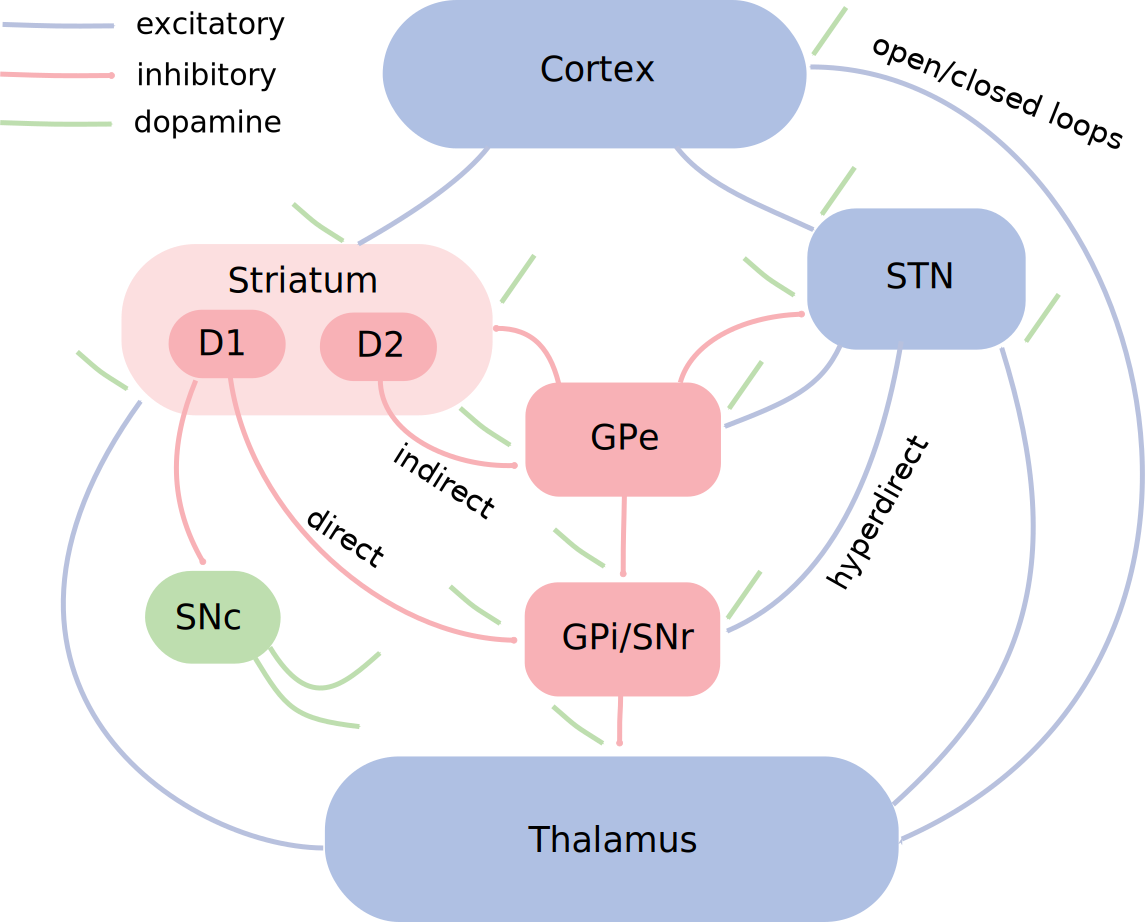
\includegraphics[width=0.6\textwidth,height=\textheight]{img/intro/bg_structure.png}

}

\caption{\label{fig-intro:bg_structure}Schematic organization of the BG.
The BG takes inputs from the cerebral cortex and tonically inhibits the
thalamus, modulating closed or open loops between the cortex and the
thalamus. The \emph{direct} pathway starts from D1-mediated MSNs of the
striatum and ends directly in the output structures GPi/SNr. The
\emph{indirect} pathway starts from D2-mediated MSNs, relays in GPe and
reaches GPi/SNr either directly or through STN. The \emph{hyperdirect}
pathway starts from STN and reaches GPi/SNr either directly or through
GPe. Dopaminergic cells in SNc have inputs from the striatum and
modulate virtually all projections within the BG.}

\end{figure}%

The \emph{hyperdirect} pathway connects directly STN to GPi/SNr through
excitatory synapses, with a much lower latency than the other pathways
(Nambu et al., 2002). It allows to send rapidly cortical information to
the output nuclei of the BG, bypassing computations in the direct and
indirect pathways. Because of its excitatory effect on GPi/SNr and the
diffuse projection of SNr on GPi/SNr (a neuron in STN excites many
neurons in GPi/SNr), it carries a ``Global No Go'' signal allowing to
suppress involuntary movements or to terminate them prematurely.
According to Nambu et al. (2002), the three pathways may cooperate
during action selection following a center-surround model: when a
voluntary movement is initiated by cortical areas, the hyperdirect
pathway first inhibits large areas of the thalamus and cerebral cortex
that are related to both the selected movement and its competitors. For
example, before moving the arm to the left, any arm movement previously
prepared will be wiped out by the increased excitation in GPi/SNr. Some
milliseconds later, the direct pathway selects the appropriate motor
program while the indirect pathway selectively inhibits competing
movements.

These three pathways form a classical feedforward view of the BG which
has been used in many models (Gurney et al., 2001a; O'Reilly and Frank,
2006; Schroll et al., 2012). As depicted in
Figure~\ref{fig-intro:bg_structure}, there exists many other projections
inside the BG which render the understanding of processing within the BG
much more complex. The thalamostriatal pathway, formed by projections
from the thalamus to the striatum, may for example be involved in
attentional processes and help the BG solve the credit-assignment
problem (Galvan and Smith, 2011). The reciprocal connections between STN
and GPe lead to oscillations under certain circumstances, what could
form the basis of an internal pacemaker inside the BG (Plenz and Kital,
1999), but can also become pathological in Parkinson's disease and
explain symptoms such as tremor (Levy et al., 2002). Much remains to be
done to fully understand the role of the STN-GPe loop (Kumar et al.,
2011). The role of the pallidostriatal projection between GPe and the
striatum is also still mainly unexplored (Bahuguna et al., 2015; Kita et
al., 1999).

\subsubsection*{Dopamine-mediated
plasticity}\label{dopamine-mediated-plasticity}
\addcontentsline{toc}{subsubsection}{Dopamine-mediated plasticity}

The striking feature of the BG is their dependency on dopamine, either
as a modulator of activity - elevated DA levels increase the
excitability of D1-mediated MSNs and decrease the one of D2 cells
(Nicola et al., 2000) - or of plasticity - different DA levels can
induce selectively \emph{long-term potentiation} (LTP) or
\emph{long-term depression} (LTD) at corticostriatal synapses (Calabresi
et al., 2007). All nuclei of the dorsal BG receive dopaminergic input
from SNc, while the ventral part receives mainly inputs from VTA.
Reciprocally, the striatum is a major source of inhibition to the
dopaminergic areas, allowing the BG to control their own dopaminergic
input (Haber et al., 2000).

Dopamine-mediated plasticity is particularly studied in the striatum.
MSNs exhibit particular dynamics: their membrane potential can be either
in a hyperpolarized \emph{down-state} or in a depolarized
\emph{up-state}. In the down-state, the excitability of the cell is very
low and striatal neurons do not emit spikes. In the up-state, the cell
is very excitable and responds to its cortical inputs. The transition
between these two states can be spontaneous (it occurs at a rate of 0.5
to 2 Hz, Leung and Yim, 1993), induced by a phasic DA burst in VTA/SNc
(Gruber et al., 2003) or by a massive cortical input (McGinty and Grace,
2009). For D1-mediated MSNs, LTP is known to occur at corticostriatal
synapses in the presence of a strong cortical input and under elevated
DA levels when the cell is in the up-state. LTD happens on the contrary
when there are weak cortical inputs, low DA levels and the cell is in
the down-state (Calabresi et al., 2007; Reynolds and Wickens, 2000). Put
together, plasticity at corticostriatal synapses seems to be driven by a
three-term DA-modulated Hebbian learning rule, where the change in
synaptic efficiency is ruled by the product of the pre-synaptic activity
(\(r^{\text{pre}}\), presence of cortical inputs), the post-synaptic
activity (\(r^{\text{post}}\), up- or down-state) and the deviation of
the dopamine level from its baseline \(\delta\):

\[
    \Delta w = \delta \cdot r^{\text{pre}} \cdot r^{\text{post}}
\]

The opposite pattern is found for D2-mediated MSNs: high DA levels
induce LTD while low levels induce LTP (Shen et al., 2008). With this
model of corticostriatal plasticity, DA becomes able to selectively
reinforce corticostriatal associations. If a motor plan selected by the
direct pathway led to reward, DA will strengthen the corticostriatal
synapses to D1-mediated MSNs that were previously activated and reduce
the ones to D2-mediated MSNs. This increases the probability that the
same motor plan will be selected again in the future by favoring the
direct pathway in its competition with the indirect one. Oppositely, if
the action leads to less reward than expected, the D1-mediated synapses
will be reduced and the D2-mediated ones increased, what strengthens the
indirect pathway and prevents further selection of that motor plan.

This mechanism of dopamine-based reinforcement in the BG further
emphasized the analogy with reinforcement learning, especially the
\emph{actor-critic} architecture (Sutton and Barto, 1998). In this
framework, the critic produces the TD error signal which is used both to
update the value of a state and to reinforce the state-action
association that led to reward. Using this error signal, the actor
simply learns to map a state onto the optimal action. In this view, the
critic would be composed by the dopaminergic system and the ventral BG,
while the actor represents a loop between the cerebral cortex and the
dorsal BG. Many neuro-computational models of the BG are based on this
architecture (Berns and Sejnowski, 1998; Gurney et al., 2001a; Houk et
al., 1995; Joel et al., 2002).

Many criticisms have been formulated to this model. First, DA cells do
not only signal RPEs but also respond to aversive, salient and novel
stimuli, which does not fit into the reward-prediction error hypothesis
(Pennartz, 1995). They also respond to reward-predicting stimuli with a
very short latency, raising the issue of how their reward-predicting
value can be predicted in such a short time (Redgrave et al., 1999). DA
is even not required for acquiring the value of a stimulus (``liking''),
only for its motivational effect (``wanting''), so the role of the
critic might be misunderstood (Berridge, 2007). Another issue with the
actor-critic assumption is the temporal credit-assignment problem:
rewards are usually delivered well after the causal action is executed.
How can this delayed feedback influence motor representations which have
long faded away?

More detailed neuro-computational models have been introduced to
overcome these issues. The PBWM (prefrontal cortex, basal ganglia
working memory) model of O'Reilly and Frank (2006) makes a strong use of
\emph{working memory} (WM) processes to bridge the temporal gap between
an action and its consequences. It furthermore provides a mechanism by
which the content of WM is gated and updated by functional loops between
the PFC and the BG. A similar approach was taken in Vitay and Hamker
(2010), which will be presented in Chapter~\ref{sec-chapter:BG}. This
model was the first to consider the importance of plasticity within the
BG (specifically in the projections from the striatum to the globus
pallidus) in addition to corticostriatal plasticity.

Generally, the role of the BG in motor learning and action selection is
partially understood, but its contribution to other forms of learning
has been less extensively studied. An interesting view considers the BG
as a fast learning device quickly acquiring rewarded associations and
transferring them to the cerebral cortex where they will be generalized
and stored in long-term memory (Ashby et al., 2005). This hypothesis is
backed up by the well-accepted role of the BG in habit formation (Seger
and Spiering, 2011). Even more generally, one can consider the BG as a
trainer for the cerebral cortex. Learning in the cerebral cortex can be
characterized as unsupervised, in the sense that cortical neurons
self-organize to represent internal and external events in the most
efficient way. Cortical areas communicate with and adapt to each other,
but there is no obvious objective function guiding the learning process
(supervised learning minimizes an error function, which is unavailable
at the cortical level), while reinforcement learning has to be ruled out
because of the slow temporal dynamics of dopamine in the cortex (the
bursts and dips of the DA signal are too smoothed out in the cortex to
carry the RPE, Seamans and Yang, 2004). The role of BG would be to
transfer specific knowledge acquired by reinforcement learning to the
more general unsupervised cortical system. In the view of Stocco et al.
(2010), the BG may also act as a conditional information-routing system,
enabling transmission between remote cortical areas and allowing the
learning of new associations.

\section{Multiple loops and organization of
behavior}\label{multiple-loops-and-organization-of-behavior}

It was mentioned that the striatum receives projections from the
entirety of the cerebral cortex. However, the organization of these
projections follows a specific topology on the surface of the striatum.
As depicted in Figure~\ref{fig-intro:Rodriguez-Oroz2009}, different
cortical regions project onto different parts of the striatum: the motor
and premotor (PMC) cortices project mainly onto the putamen, the
dorsolateral prefrontal cortex (dlPFC) projects mainly on the caudate
nucleus, while the orbitofrontal (OFC) and ventromedial prefrontal
(vmPFC) cortices project mainly on the nucleus accumbens. As this
segregation is preserved throughout the BG, from the projections of the
striatum on the GP to the thalamic nuclei relaying the output of the BG
back to the cortex, the prefrontal cortex / basal ganglia system is said
to be organized in parallel segregated loops (Alexander et al., 1986).

\begin{figure}

\centering{

\includegraphics{img/intro/Rodriguez-Oroz2009.jpg}

}

\caption{\label{fig-intro:Rodriguez-Oroz2009}Parallel segregated loops
between the cerebral cortex and the BG. The motor loop starts from the
motor and premotor cortices and involves mainly the putamen. The
associative (or cognitive) loop involves the dorsolateral cortex and the
caudate nucleus. The limbic loop involves the orbitofrontal and
ventromedial cortices to the ventral striatum (nucleus accumbens).
Adapted from Rodriguez-Oroz et al. (2009).}

\end{figure}%

Each loop is therefore specialized in a particular functional domain:
the motor loop is involved in motor learning and action selection, the
associative loop in cognitive processes such as sequence learning and WM
updating, the limbic loop in motivation and goal-directed learning.
These subdivisions can be further refined: the motor loop is in fact
composed of multiple segregated loops depending on the cortical region
of origin (M1, SMA, pre-SMA\ldots). Other loops have been identified,
such as the oculomotor loop, devoted to the control of eye movements, or
the visual loop, linking the inferotemporal and medial temporal cortices
to the tail of the caudate nucleus. The importance of the visual loop
will be explained in Chapter~\ref{sec-chapter:PRh} and
Chapter~\ref{sec-chapter:BG}. A similar topological segregation can
further be extended to the projections within a functional loop: the
topology of the cortical area (e.g.~the somatotopic representation of
body parts in the motor cortex) is preserved inside the BG (Nambu,
2011). In this view, the PFC/BG system is composed by thousands of small
parallel loops (O'Reilly and Frank, 2006).

The segregation is however not total: a certain degree of overlap is
observed in the corticostriatal projections, allowing for example parts
of the striatum to integrate both motor and associative information. The
funneling structure of the BG - there are 100 times more neurons in the
striatum than in GPi/SNr - also increases the probability that the loops
communicate with each other inside the BG (Bar-Gad et al., 2003).
Finally, the thalamic nuclei relaying the output of the BG back to the
cortex do not target only the original cortical area, but reach also
adjacent ones. In the PFC / BG system, one distinguishes \emph{closed
loops}, where a single cortical area projects to the striatum and
receives the processed information back, from \emph{open loops}, where a
cortical area sends information to the BG and the result is
``forwarded'' to another cortical area (Ebner et al., 2015). Category
learning in the visual loop between the inferotemporal cortex and the BG
is for example transferred to the motor cortex through an open loop
(Seger, 2008). The exact organization of the PFC / BG system into closed
and open loops is still not precisely known, but this is an important
mechanism by which the BG can modulate information transmission in the
prefrontal cortex (Stocco et al., 2010).

The question that arises is how these multiple loops could learn useful
associations in their respective domains based on a single unitary
reward-prediction error signal, as hypothesized by the TD analogy. SNc
and VTA actually display a complex topological organization depending on
their reciprocal connections with the striatum (striato-nigro-striatal
system, Haber et al., 2000). As depicted in
Figure~\ref{fig-intro:daloops}, each region of the striatum engaged in a
closed loop with the cerebral cortex forms reciprocal connections with a
specific region of the SNc/VTA dopaminergic areas: the striatum sends
inhibitory connections to SNc/VTA, which returns a dopaminergic signal.
However, each striatal region also projects on the adjacent dopaminergic
region along a rostro-caudal axis, i.e.~from limbic to associative to
motor domains. This pattern on connectivity forms a spiraling structure
which allows different striatal regions to influence others by
modulating their dopaminergic inputs.

\begin{figure}

\centering{

\includegraphics[width=0.7\textwidth,height=\textheight]{img/intro/daloops.png}

}

\caption{\label{fig-intro:daloops}Spiraling connectivity pattern in the
striato-nigro-striatal system. Different cortical areas (here, vmPFC,
OFC, dACC - the dorsal anterior cingulate cortex -, dlPFC and SMC - the
supplementary motor area) form closed loops with different parts of the
striatum (ventral for vmPFC and OFC, dorsal for the others) following a
rostro-caudal axis. Each part of the striatum projects on specific
regions of the SNc/VTA system, which reciprocate the connections.
However, they also project on adjacent dopaminergic regions in the
caudal direction, forming a spiraling structure allowing the different
closed loops to communicate through dopaminergic activity. Adapted from
Keramati and Gutkin (2013).}

\end{figure}%

The resulting organization of PFC-BG loops along a
limbic-associative-motor gradient has fundamental consequences on
goal-directed behavior. Limbic regions, critical for motivational and
affective processes, are in a position to influence how cognitive plans
are formed and learned by associative regions, which themselves control
how individual movements and actions are executed in motor regions. This
highlights the tight integration between cognitive and emotional
processes: goals are mainly represented in OFC, which is strongly
connected with the limbic system (amygdala, ventral BG) and influences
cognitive processes in dlPFC. Based on neuro-anatomical evidence, the
classical view opposing cognition and emotion as competitors to produce
behavior has to be replaced by an emphasis on the cooperation between
the two systems.

This gradient also has consequences on learning: striatal regions
associated to goal-directed learning influence plasticity in striatal
regions associated to habit formation (Khamassi and Humphries, 2012; Yin
et al., 2004). This provides a mechanism by which flexible behaviors
acquired through goal-directed learning can be transferred into
procedural memory to become habits. Similarly, Pavlovian-to-Instrumental
transfer (PIT) is the ability to transfer stimulus values acquired
through Pavlovian conditioning to instrumental behavior: after a first
phase of operant conditioning where a rat learns to press levers to
obtain different outcomes (say, food and water), a classical
conditioning phase is introduced, pairing initially neutral stimuli
(tone or light) to the same outcomes. The effect of PIT is that, when
back in the operant conditioning room, the conditioned stimuli will now
trigger the lever press leading to the same outcome (Corbit and
Balleine, 2011). The mechanisms allowing a transfer of learning between
classical and instrumental conditioning happen in the cooperation
between two loops within the ventral BG, involving two parts of the
nucleus accumbens, the core and the shell (Gruber and McDonald, 2012).

Although the concept of multiple parallel PFC/BG loops has been often
used in neuro-computational models (N'guyen et al., 2014; e.g. Nakahara
et al., 2001; O'Reilly and Frank, 2006), only a few have used the
underlying limbic-associative-motor gradient in dopaminergic
connectivity to investigate the organization of behavior. Keramati and
Gutkin (2013) for example studied this system to explain the mechanisms
of addiction. In Schroll et al. (2012) (Chapter~\ref{sec-chapter:WM}),
we proposed a neuro-computational model of working memory formation and
maintenance involving three PFC/BG loops, two associative and one motor,
which coordinate their learning through the spiraling
striato-nigro-striatal system. The dopaminergic system has a central
role in organizing behavior and learning; very simplified models such as
TD actually limit our ability to understand the underlying processes.

\section{Structure of the thesis and
contribution}\label{structure-of-the-thesis-and-contribution}

This thesis is composed of five articles published in international
peer-reviewed journals. They were selected to be representative of the
different aspects of my research on the role of dopamine in motivated
behavior. In Vitay and Hamker (2008) (Chapter~\ref{sec-chapter:PRh}), we
studied the influence of dopamine on memory retrieval in the perirhinal
cortex, a part of the temporal lobe involved in object recognition and
visual memory. In Vitay and Hamker (2010)
(Chapter~\ref{sec-chapter:BG}), we designed a neuro-computational mode
of the BG which is able to solve delayed rewarded visual memory tasks.
This fundamental model was the first to introduce plasticity within the
BG and was further extended in collaboration with Dr.~Henning Schroll to
account for working memory formation Chapter~\ref{sec-chapter:BG}. In
Vitay and Hamker (2014) (Chapter~\ref{sec-chapter:VTA}), we designed a
detailed model of the dopaminergic system during conditioning, with a
strong emphasis on its dependency on timing processes. Additionally, in
Vitay et al. (2015) (Chapter~\ref{sec-chapter:ANNarchy}), we present a
neural simulator that was developed in parallel and which allows to
define these neuro-computational models easily and simulate them
efficiently on parallel hardware. A detailed description of the content
of these articles is provided in the following sections.

\subsection*{List of publications included in the
thesis}\label{list-of-publications-included-in-the-thesis}
\addcontentsline{toc}{subsection}{List of publications included in the
thesis}

\begin{enumerate}
\def\labelenumi{\arabic{enumi}.}
\item
  Vitay, J. and Hamker, F. H. (2008). Sustained activities and retrieval
  in a computational model of the perirhinal cortex. \emph{Journal of
  Cognitive Neuroscience}, 20, 11, 1993-2005, doi:
  \href{http://www.mitpressjournals.org/doi/abs/10.1162/jocn.2008.20147}{10.1162/jocn.2008.20147}
\item
  Vitay, J. and Hamker, F. H. (2010). A computational model of basal
  ganglia and its role in memory retrieval in rewarded visual memory
  tasks. \emph{Frontiers in Computational Neuroscience}, 4, doi:
  \href{http://dx.doi.org/10.3389/fncom.2010.00013}{10.3389/fncom.2010.00013}
\item
  Schroll, H., Vitay, J., and Hamker, F. H. (2012). Working memory and
  response selection: a computational account of interactions among
  cortico-basalganglio-thalamic loops. \emph{Neural Networks}, 26,
  59--74, doi:
  \href{http://dx.doi.org/10.1016/j.neunet.2011.10.008}{10.1016/j.neunet.2011.10.008}
\item
  Vitay, J. and Hamker, F. H. (2014). Timing and expectation of reward:
  a neuro-computational model of the afferents to the ventral tegmental
  area. \emph{Frontiers in Neurorobotics}, 8, 4, doi:
  \href{http://dx.doi.org/10.3389/fnbot.2014.00004}{10.3389/fnbot.2014.00004}
\item
  Vitay, J., Dinkelbach, H. Ü., and Hamker, F. H. (2015). ANNarchy: a
  code generation approach to neural simulations on parallel hardware.
  \emph{Frontiers in Neuroinformatics}, 9, 19,
  doi:\href{http://dx.doi.org/10.3389/fninf.2015.00019}{10.3389/fninf.2015.00019}
\end{enumerate}

\subsection*{Contribution to each
article}\label{contribution-to-each-article}
\addcontentsline{toc}{subsection}{Contribution to each article}

I am the primary author of articles 1, 2 and 4, having conducted the
research, implemented the models, performed the experiments, analyzed
the results and primarily written the manuscripts. Prof.~Hamker
supervised the research, guided the whole process and participated in
the writing. For article 3, Dr.~Henning Schroll is the primary author.
He implemented the model, ran the experiments, analyzed the results and
primarily wrote the article. I co-supervised the development of the
model together with Prof.~Hamker and participated in the writing. For
article 5, Helge Ülo Dinkelbach was involved in developing the neural
simulator and running the experiments, co-supervised by Prof.~Hamker and
me. I developed equally the neural simulator and wrote primarily the
manuscript.

\subsection{Chapter 2 : Perirhinal cortex and
dopamine}\label{chapter-2-perirhinal-cortex-and-dopamine}

Working memory is the ability to temporarily store and manage
information in order to use it for cognitive processes (Baddeley, 1986).
A typical example is remembering a phone number before typing it: the
number is stored in short-term memory as long as it is needed for the
action, but the memory fades away when it is not required anymore. The
neural correlate of WM processes is \emph{sustained activation}: neurons
which are activated by the presence of the information stay active
during the whole period between its disappearance and its later use by
cognitive processes. Sustained activation has been found in many brain
areas, including the prefrontal cortex (Funahashi et al., 1989), the
parietal cortex (Koch and Fuster, 1989), the inferotemporal cortex
(Ranganath et al., 2004) and the medial temporal lobe (Naya et al.,
2003). The medial temporal lobe (MTL) has an important role in
interfacing high-level visual information represented in the
inferotemporal cortex (IT) with long-term mnemonic information encoded
in the hippocampal formation. It is composed of the perirhinal (PRh),
entorhinal (ERh) and parahippocampal (PHC) cortices.

PRh is in particular involved in visual object categorization (Murray
and Richmond, 2001), multimodal integration (Taylor et al., 2006),
long-term memory encoding (Buffalo et al., 2000) and retrieval (Brown
and Xiang, 1998). In visual object categorization, PRh develops
view-independent representation of objects: objects are in general seen
from particular angles or are only partially visible. PRh learns to
integrate over time these different views and bind them together in a
unitary representation. In the model of PRh we developed (Vitay and
Hamker, 2008), PRh is represented by two populations of excitatory and
inhibitory neurons, respectively, with biologically plausible
proportions and connectivity. Different objects are presented to the
model through connections from a model of IT to the excitatory neurons.
Each object is composed of different parts, which are randomly selected
at each presentation: for example the first presentation of a chair
would contain its right side and three feet, the second would be its
back and only two feet, and so on. Through plasticity in the lateral
connections between the excitatory neurons, we observe the formation of
connected clusters of neurons which represent the object as whole:
individual neurons of the cluster receive visual input from only one
part of the object, but they have become connected to neurons
representing all the other parts of the object.

Sustained activation has been observed in PRh during delayed
matching-to-sample (DMS) tasks, where a visual object (the sample) is
shortly presented and removed for a variable duration called the delay
period. The same or a different object (the match) is then presented and
the subject has to respond if the new object matches the sample. PRh
neurons representing the sample object stay active during the delay
period (Nakamura and Kubota, 1995). The model reproduces this effect by
incorporating the effect of DA on synaptic transmission in the cortex,
extrapolated from its known influence in the prefrontal cortex
(Durstewitz et al., 2000; Seamans and Yang, 2004). We observed that PRh
neurons show sustained activation under intermediate levels of DA, but
not low or high doses, a phenomenon known as \emph{inverted-U curve} in
the prefrontal cortex (Vijayraghavan et al., 2007). Moreover,
intermediate levels of DA favor the propagation of activity within a
cluster: while at low DA levels only the neurons receiving visual
information get activated, the whole cluster gets activated at
intermediate levels because of the enhanced lateral connections within
the cluster. Instead of representing a partial view of the object, PRh
represents all possible views at the same time, leading to a complete
representation of the object. This provides a mechanism by which DA
modulates processing in PRh and allows memory retrieval.

The mechanisms used in this model are a very important step for visual
processing as they allow view-invariant representations of an object to
be formed and retrieved by cognitive processes. Under optimal DA levels,
object representations can be completed and help categorization.
Furthermore, the visual template representing an object in PRh can be
activated by cognitive processes (either through direct projections from
the PFC or through the thalamus) and used to guide visual search. The
visual system is principally organized in two separate pathways: the
ventral pathway, originating in the primary visual cortex (V1) and
ending in the inferotemporal lobe, is specialized in object recognition;
the dorsal pathway, originating in V1 and ending in the parietal cortex,
focuses on the localization of visual objects and their manipulation
(Ungerleider and Mishkin, 1982). Activating a template in PRh biases IT
toward the characteristic features of this object, which itself biases
representations in the ventral pathway through feedback projections.
Once the corresponding features are enhanced in V1, the dorsal pathway
can then locate the object and direct an action toward it (Hamker,
2004a; Hamker, 2005b). Understanding how visual templates are formed and
retrieved is a first step toward understanding the cognitive control of
vision.

\subsubsection*{Insights on the role of
DA}\label{insights-on-the-role-of-da}
\addcontentsline{toc}{subsubsection}{Insights on the role of DA}

Tonic levels of DA control the processing properties of PRh by switching
from a representational mode - only the perceived information is
represented - to a mnemonic one - visual templates are completed or
retrieved.

\subsection{Chapter 3 : Basal ganglia and memory
retrieval}\label{chapter-3-basal-ganglia-and-memory-retrieval}

Maintaining visual templates in PRh is a critical component of delayed
rewarded tasks such as delayed match-to-sample (DMS, reward is delivered
if a response is made when the target matches the sample), delayed
non-match-to-sample (DNMS, the response is rewarded only if the target
does not match the sample) or delayed pair-association (DPA, similar to
DMS but there is a an arbitrary association between the sample and the
rewarded target - e.g.~respond for an apple when the sample is a car).
The visual loop of the BG, linking high-level visual cortical areas such
as IT and PRh with the body and tail of the caudate nucleus, is involved
in selectively activating visual templates during the delay period of
such tasks in order to prepare the correct response (Levy et al., 1997).
The major difficulty of these three tasks is that the visual template to
be activated can be different from the presented sample, so the target
has to be retrieved from memory.

In Vitay and Hamker (2010), we developed a neuro-computational model of
the visual loop of the BG. It is composed of a closed loop between PRh,
the caudate nucleus, SNr and the ventro-anterior thalamus, and an open
loop with a projection from the dlPFC to the caudate nucleus. Contrary
to the generic scheme described on Figure~\ref{fig-intro:bg_structure},
we only modeled the direct pathway of this loop. In the experimental
setup, a sample is first presented and stored in dlPFC. After a delay of
150 ms, a cue indicated which task to perform (DMS, DNMS or DPA) is
presented and stored in dlPFC. Finally, after another delay, two stimuli
are presented: the target (which matches the sample depending on the
task) and a distractor. After a delay, we measure the maximal activity
in PRh and deliver reward to SNc if the target has a higher activity.
The dopaminergic signal in SNc in response to the reward modulates
learning at corticostriatal synapses (both from PRh and dlPFC) according
to the three-term DA-modulated Hebbian learning rule presented in this
chapter. This is in line with many models of the BG (e.g. Brown et al.,
1999; O'Reilly and Frank, 2006). The novelty of this model is that DA
also modulates plasticity within the BG, in the connections from the
striatum to SNr as well as in the lateral connections of SNr.

This internal plasticity, confirmed by experimental evidence
(Rueda-Orozco et al., 2009), releases the constraints on the striatum.
In other models, each striatal region converges on a small number of
GPi/SNr cells, allowing to disinhibit a single action. The
corticostriatal projections must therefore solve two different problems:
integrating different cortical representations (here, the sample and the
task cue) and map them on the correct action. If plasticity in the
projection between the striatum and GPi/SNr is added, corticostriatal
projections only need to map cortical associations on the striatum (a
form of self-organization), while the striatopallidal ones learn to map
these representations onto the correct action. Additionally, plasticity
within SNr ensures selectiveness in the output of the BG.

The resulting model is able to learn through reinforcement learning the
three tasks using a limited number of objects. It provides a novel
mechanism by which cognitive processes in the PFC can learn to influence
visual processing by retrieving visual templates. Two limitations of
this model should be outlined: first, it only considers the direct
pathway of the BG, neglecting the indirect and hyperdirect ones; second,
the mechanisms to encode the sample and the task cue in working memory
in dlPFC are hard-coded and not learned. The first limitation was since
overcome by an extension of this model including the indirect and
hyperdirect pathways, with a strong emphasis on the dopamine-modulated
plasticity in these pathways. This extended model was successfully used
to explain cognitive deficits in various BG-related diseases, such as
Parkinson's disease (Schroll et al., 2014) and Huntington's disease
(Schroll et al., 2015). Flexible WM mechanisms to learn to maintain
relevant information in dlPFC are presented in the next section (Schroll
et al., 2012).

\subsubsection*{Insights on the role of
DA}\label{insights-on-the-role-of-da-1}
\addcontentsline{toc}{subsubsection}{Insights on the role of DA}

Dopamine regulates plasticity in the projections to the BG, but also
between the different nuclei of the BG. Its phasic component carries a
reward-prediction error that reinforces successful stimulus-response
associations. DA-mediated plasticity occurs only in the acquisition
phase, when the success of a response is not predicted yet. When a
striatal representation is associated with reward delivery, it cancels
dopaminergic activation and suppresses learning.

\subsection{Chapter 4 : WM and multiple basal ganglia
loops}\label{chapter-4-wm-and-multiple-basal-ganglia-loops}

Updating and maintaining information in WM is a complex cognitive
process involving mainly the dlPFC and the BG (Frank et al., 2001),
although many other cortical areas play a significant role (Ashby et
al., 2005; Jonides et al., 1998). Many neuro-computational models
consider that the BG is involved only in WM updating, i.e.~the
conditional entry of stimuli into it (Helie et al., 2013; Uttal, 2015).
One of the most prominent models of WM (O'Reilly and Frank, 2006) for
example considers the BG as a gating mechanism allowing, based on
reinforcement learning, sensory information to enter recurrent loops
within the PFC. It has among others been applied to the complex 1-2-AX
task, which can be described as followed: a sequence of letters (A, B,
X, Y) and digits (1, 2) is displayed on a screen. The subjects have to
respond with the left button if they see an A followed by an X, but only
if the last digit they saw was a 1. If that last digit was a 2, they
have to press left when they see a B followed by a Y. In all other
cases, they have to press right.

The 1-2-AX task is very complex, even for humans. It involves
maintaining two levels of information in WM: what was the last digit I
saw (outer loop) and have I just seen an A or a B (inner loop)? If these
two pieces of information are kept in WM, deciding whether to press left
or right when an X or Y appears becomes as trivial as a
stimulus-response association. The difficulty is to know how a system
can learn to maintain the outer and inner loops based solely on
reinforcement learning, i.e.~without explicit knowledge of the task.
O'Reilly and Frank (2006) solve the problem by implementing three
parallel PFC/BG loops, one learning to maintain 1 and 2, another A and B
and the last one X or Y. The structural credit assignment problem - if
the response is incorrect, which of these three loops has failed? - is
solved by allowing each loop to modulate its own dopaminergic reward
signal, but these loops are mostly independent of each other. Moreover
the BG are only used to update WM content, not actually maintain it,
contrary to experimental evidence (Landau et al., 2009).

In Schroll et al. (2012), we proposed a neuro-computational model of WM
updating and maintenance involving three PFC-BG loops: two associative
loops and a motor one. The role of the motor loop is to decide which
motor response (left or right) should be executed based on short-term
mnemonic information maintained in the associative loops during a 1-2-AX
task. The role of the two associative loops is to learn to maintain the
outer (1 and 2) and inner (A and B) loops, respectively. Based on an
idea by Krueger and Dayan (2009), we posit that shaping plays an
important role in organizing the different loops: animals usually don't
address complex cognitive tasks directly, but incrementally generate
more and more complex behavior by reusing abilities that were previously
acquired. In the case of the 1-2-AX task, this would correspond to
responding first to a 1 or 2, then to 1 followed by A or 2 followed by
B, and finally by the 1-2-AX task task itself. Once a subtask is
mastered, errors in performance can be interpreted as a change in task
complexity, signaling that more cognitive resources should be allocated
to solve the problem.

In the first shaping phase (only digits are presented), the motor PFC/BG
loop learns to respond appropriately using the same mechanisms as in
Vitay and Hamker (2010). When the second phase is introduced (A-X or
B-Y), the motor loop can not solve the problem because it has no memory
of the last digit seen. One of the two associative loops then starts
learning to maintain this information through a closed loop. The
sustained activation of a digit then biases the motor loop to respond
correctly to a 1-A or 2-B association. Finally, when the full 1-2-AX
task is introduced, the associative and motor loops fail again, as only
the outer loop is maintained. The associative loop sends a ``distress''
signal, telling the other associative loop to help solve the task. The
new loop then learns to maintain A and B, providing enough information
to the motor loop to execute the correct motor response.

Associative PFC/BG loops learn from errors as long as they are not
confident in their output. When they become confident but the whole
behavior fails, they ask for more cognitive resources to be allocated to
the task instead of simply unlearning what they were previously
correctly doing. Communication between the loops and the subsequent
recruitment of cognitive resources is based on the spiraling
striato-nigro-striatal connectivity (Haber et al., 2000): each loop has
its own dopaminergic signal, which can be activated by loops higher in
the hierarchy. When the first associative loop fails to solve the task
although it was previously performing well, it signals the second loop
through its dopaminergic system that it should get engaged in order to
improve the organism's ability to acquire rewards.

Monitoring of performance is a crucial mechanism by which cognitive
resources can be allocated to solve a problem. The brain does not
relearn everything every time it is confronted with a new problem, it
first tries already acquired solutions and only tries to combine or
update them when the performance is not satisfying (Botvinick et al.,
2009). Based on neuro-anatomy and the functional importance of dopamine
in goal-directed behavior, the spiraling structure of the
striato-nigro-striatal system is a good candidate to coordinate the
flexible recruitment of PFC-BG loops. However, the anterior cingulate
cortex (ACC) is known to be crucial in self-performance assessment and
error monitoring. As ACC is involved in a PFC-BG loop located just in
between the limbic regions (OFC, vmPFC) and the associative ones (dlPFC)
(Haber and Knutson, 2010), its dominating position may be the crucial
link to determine the involvement of different associative loops to
solve cognitive problems. In all cases, understanding how the
dopaminergic system processes reward expectations and errors in these
different loops is important for the understanding of the organization
of PFC-BG loops.

\subsubsection*{Insights on the role of
DA}\label{insights-on-the-role-of-da-2}
\addcontentsline{toc}{subsubsection}{Insights on the role of DA}

The activation of dopaminergic neurons is not uniform but specific to
each PFC-BG loop. Different loops can control their learning ability by
modulating their influx of dopamine. Moreover, the hierarchical
organization of the reciprocal connections between the striatum and the
dopaminergic areas allows the flexible recruitment of cognitive
resources when needed.

\subsection{Chapter 5 : Timing and expectation of
reward}\label{chapter-5-timing-and-expectation-of-reward}

The TD error signal depends only on two pieces of information: the
prediction of the value of a state (or action) and the reward actually
received. As shown on Figure~\ref{fig-intro:vta_afferents}, VTA receives
information from many other brain regions: a massive inhibitory
projection from NAcc (possibly excitatory through a relay on the ventral
pallidum - VP), direct cortical excitation from the PFC, excitatory
connections from reward-related brainstem regions such as the
pedunculopontine tegmental nucleus (PPTN), the lateral habenula (LHb) or
the lateral hypothalamus (LH). As discovered recently, it also receives
inhibitory connections from the mesopontine rostromedial tegmental
nucleus (Bourdy and Barrot, 2012; RMTg, Jhou et al., 2009). Inhibitory
neurons in the VTA furthermore control the activity of VTA cells and
project on NAcc and PFC. The complexity of the afferent system to VTA
suggests that it computes more than a simple reward-prediction error
signal.

\begin{figure}

\centering{

\includegraphics[width=0.6\textwidth,height=\textheight]{img/intro/vta_afferents.png}

}

\caption{\label{fig-intro:vta_afferents}Major afferent areas to VTA. The
prefrontal cortex (PFC), the basolateral amygdala (BLA), the ventral
subiculum of the hippocampus (vSub/Hipp) project on the nucleus
accumbens (NAc), which has a strong inhibitory influence on VTA. VTA
also receives direct excitatory connections from the PFC. The
pedunculopontine tegmental nucleus (PPTg), laterodorsal tegmental
nucleus (LDT), lateral hypothalamic and lateral preoptic areas
(LHA/LPOA), lateral habenula (LHb), among others, also provide
excitatory inputs to the dopaminergic cells of VTA. The mesopontine
rostromedial tegmental nucleus (RMTg) provides inhibitory input. VTA
also comprises GABAergic cells, which inhibit the dopaminergic ones as
well as the PFC and NAc. Adapted from Sesack and Grace (2010).}

\end{figure}%

Several neuro-computational models of the dopaminergic system have been
proposed to explain this organization (Brown et al., 1999; O'Reilly et
al., 2007; Tan and Bullock, 2008). A common point of these
\emph{dual-pathway} models is that they distinguish the excitatory and
inhibitory components driving VTA activity for rewards and
reward-predicting stimuli, although some debate exists on the exact
structures carrying these informations. The DA burst in response to
delivery of reward likely originates from the PPTN, while the
cancellation of this response when the reward is fully predicted
originates from the striatum. Reward-predicting stimuli activate VTA
either though the excitatory projection from PFC or from the amygdala.
The main difference between those models is how the temporal component
of the DA signal is computed: in the experiments of Schultz et al.
(1997), VTA shows a dip below baseline at the exact time where a reward
was expected but did not occur. As no sensory event happens at this
time, this indicates that internal timing mechanisms are involved in
generating the DA signal.

The hypothesis taken by Brown et al. (1999) and Tan and Bullock (2008)
is that the striatum implements a \emph{spectral timing} mechanism
(Grossberg and Schmajuk, 1989) where striatal neurons have intracellular
calcium levels which peak at different times after stimulus onset:
detecting these peaks allows to estimate the time elapsed since onset.
Because of the lack of evidence for such a mechanism, we decided in
Vitay and Hamker (2014) to investigate alternative mechanisms for
interval timing. A successful model of interval timing is the
\emph{Striatal-Beat Frequency} model (Matell and Meck, 2004). The basic
principle is that cortical neurons behave as oscillators at different
frequencies which are synchronized at stimulus onset. The population
code composed by these oscillators provides a unique description of the
time elapsed since onset: if enough neurons and a large enough range of
frequencies are used, the population will never display twice the same
pattern, while being reproducible between different trials. Striatal
neurons can then detect the elapsed duration by learning to respond to
the cortical pattern present when reward is delivered: the DA burst at
reward delivery influences plasticity at corticostriatal synapses so
they become selective only for that pattern. This model captures many
aspects of the link between dopaminergic activity and timing processes,
including the accelerated sense of time when DA is elevated - for
example in aroused states or during recreational drug use - or the
effect of lesions of SNc/VTA or the striatum on interval timing (Coull
et al., 2011).

Using this hypothesis, we developed a novel neuro-computational model
shedding new light on the afferent system to VTA based on
neuro-anatomical evidence. Although the response to primary rewards is
classically mediated through PPTN, we propose that conditioned stimuli
activate VTA through the existing connection between the amygdala - a
structure known for its involvement in classical conditioning - and
PPTN. Furthermore, we propose that the cancellation of the DA burst when
a reward is predicted and the DA dip when a reward is omitted are
processed by two different mechanisms: the direct inhibitory projection
from NAcc to VTA can inhibit the response to primary rewards, but
bringing VTA activity below baseline requires a complex sub-network
linking the ventral BG (NAcc and VP) to VTA through LHb and RMTg.

The model is able to reproduce a wealth of experimental findings: the
progressive appearance of phasic bursts at CS onset through classical
conditioning, the progressive canceling of the amplitude of the phasic
bursts elicited by primary rewards, the strong phasic inhibition at the
time when reward is expected but not delivered, the dependency on reward
magnitude of the activities in BLA and VTA, the response to reward
delivered earlier than expected (Fiorillo et al., 2003; Pan and Hyland,
2005; Schultz et al., 1997). This model is currently limited to VTA
activity during classical conditioning but provides a detailed
functional basis to address the mechanisms of dopamine release in the
PFC-BG system.

\subsubsection*{Insights on the role of
DA}\label{insights-on-the-role-of-da-3}
\addcontentsline{toc}{subsubsection}{Insights on the role of DA}

The dopaminergic system integrates information from diverse structures,
signaling reward delivery, prediction and omission through different
projections. Cognitive, motor and emotional information converge on the
dopaminergic system, which then redistributes back the most relevant
aspects. It is critically involved in timing processes and therefore the
organization of behavior through time.

\subsection{Chapter 6 : Neural simulator
ANNarchy}\label{chapter-6-neural-simulator-annarchy}

Neuro-computational models are described by a limited set of
information:

\begin{enumerate}
\def\labelenumi{\arabic{enumi}.}
\tightlist
\item
  The number of populations of neurons (or areas), the number of neurons
  in each population and possibly a topology;
\item
  A set of ordinary differential equations (ODE) describing the dynamics
  of each neuron model in the model;
\item
  Connectivity patterns for the projections between the populations:
  all-to-all, probabilistic, distance-based, etc;
\item
  A set of ODEs describing the dynamics of synaptic plasticity for the
  projections;
\item
  Methods to provide inputs and read out outputs of the network.
\end{enumerate}

Some of these informations can be inferred from anatomical and
physiological data. Neural and synaptic dynamics are well studied, so
only small modifications usually need to be applied to standard models.
The main difficulty is actually to find sensible values for the free
parameters of the model: time constants, learning rates, etc. Although
experimental data constrain the range of possible values, this is the
most time-consuming part of the design of a neuro-computational model.

Another difficulty is that neural networks can very quickly become
expensive to simulate: the number of connections grow quadratically with
the number of neurons and the computations can become very slow if no
special care is taken about the optimality of the implementation.
Parallel computing offers many advantages for the simulation of neural
networks as each neuron only processes local information, but writing
optimized parallel code on different hardware (shared-memory systems,
distributed systems or recently general-purpose graphical cards - GPU)
can be quite difficult and time-consuming.

Consequently, researchers in computational neuroscience use neural
simulators instead of writing their own simulation code. These are
libraries allowing the definition of a model, usually in a high-level
scripting language such as Python or Matlab, and hiding from the user
all the low-level implementation details necessary to run efficiently
simulations in parallel. Another positive side effect is that neural
simulators facilitate the exchange of models between researchers for
validation and the integration of different models to obtain more
functionalities.

Many different neural simulators are available to the community: NEURON,
NEST, GENESIS, Brian, GeNN, Auryn Vitay et al. (2015). They all have
different strengths and drawbacks: the exhaustiveness of the set of
neural and synaptic models which can be included in a model, the
simplicity of the interface, their optimization for a particular
parallel hardware, etc. These simulators focus on the simulation of
spiking networks, where neurons exchange information through discrete
events (spikes), while rate-coded models, where neurons exchange
directly a firing rate, are usually impossible or very difficult to
define. At the exception of Brian, these simulators provide a fixed set
of neural and synaptic models which can only be extended with great
difficulty: as long as one only needs standard models, these simulators
are very practical, but if one wants to investigate new mechanisms, the
programming effort becomes important. Brian proposes a very flexible
code generation approach, where neural and synaptic dynamics are
described using a text-based equation-oriented mathematical description
which is used to generate Python code at run-time (Stimberg et al.,
2014). Using code generation allows the user to define virtually any
neural or synaptic model.

In parallel to the design of the neuro-computational models presented
above, I developed over several years a neural simulator named ANNarchy
(Artificial Neural Networks architect), later in collaboration with
Helge Ülo Dinkelbach. Two main principles guided the development: first,
it should allow the rapid definition of neural networks, for both
rate-coded and spiking models. Second, the simulation should be able to
run transparently and efficiently on different parallel hardware (using
OpenMP for shared-memory systems, MPI for distributed ones and CUDA for
GPUs). Code generation is the core principle of the simulator: the
definition of the network in a Python script is analyzed and used to
generate entirely the simulation code (including a translation from the
text-based description of ODEs to executable code statements), using
templates adapted to the parallel framework.

In Vitay et al. (2015), we presented the neural simulator to the
community and showed that its parallel performance is at least
comparable to the alternatives. It is freely available and released
under an open-source license. In addition to being used inside the
professorship of Artificial Intelligence of the TU Chemnitz, several
research groups have shown interest in this simulator and have started
using it for their own research. More than just a tool, ANNarchy is also
a very promising platform to study the issues raised by
neuro-computational models to the parallel computing community: relying
on code generation, it allows to explore systematically the different
optimizations and algorithms that allow specific networks to be
simulated efficiently on different hardware.

\section{Conclusion}\label{conclusion}

The common theme of this thesis is the role of dopamine in the
cognitive, motor and emotional processes involved in goal-directed
behavior. Using biologically-realistic neuro-computational models, I
investigated its role in visual object categorization and memory
retrieval (Vitay and Hamker, 2008), reinforcement learning and action
selection (Vitay and Hamker, 2010), the updating, learning and
maintenance of working memory (Schroll et al., 2012) and timing
processes (Vitay and Hamker, 2014). The involvement of dopamine in such
a wide variety of processes highlights the importance of understanding
the mechanisms leading to dopamine release as well as its effect on the
activity and plasticity of cortical and subcortical structures.

The different models outline different facets of the effect of DA
release in the brain. In the cerebral cortex, the most important effect
of DA is the modulation of synaptic transmission in localized networks
of excitatory and inhibitory neurons. DA release in the prefrontal
cortex influences short-term memory processes by inducing two modes of
computation: an ``open gate'' mode, where multiple sensory information
can enter the neural substrate and be represented in parallel; and a
``closed gate'' mode, where only the strongest and most important
representation is maintained, allowing sustained activation (Seamans and
Yang, 2004). The transition between these two modes follows an inverted
U-curve, where low and high DA levels lead to open gates and
intermediate levels to closed gates. The proposed model of PRh (Vitay
and Hamker, 2008) exhibits a similar mechanism: PRh can switch between a
representational state (driven by inputs) and a mnemonic state (where
visual memory is retrieved) depending on the modulatory influence of DA
on synaptic transmission. It is likely that DA is able to induce such
different modes of computation in all cortical areas receiving
dopaminergic input (the whole frontal lobe, the inferotemporal and
parietal cortices). The functional consequences of this property still
need to be explored, especially with respect to the spatial scale: do
all these cortical areas receive the same dopaminergic input from VTA,
or is there a functional topology allowing to selectively switch single
areas?

In the basal ganglia, the main mode of action considered in the models
is the inducement of plasticity by phasic DA bursts or dips. These
short-term deviations around the baseline shape synapses coming from the
cortex, but also inside the BG. Although more complex models of
plasticity have been used, their influence basically follows a
three-term DA-modulated Hebbian learning rule. DA bursts reinforce
PFC/BG representations which lead to reward, while DA dips ``punish''
the ones which led to omission of reward or punishment (Schroll et al.,
2012; Vitay and Hamker, 2010). This mechanism is fundamentally in line
with actor/critic analogies. The short-term duration and the short
latency of these phasic responses furthermore allow DA to signal
precisely the occurrence of meaningful events, what can be used to learn
time intervals and provide an internal sense of elapsed time (Vitay et
al., 2015). One aspect of dopamine that will be addressed by future work
is the influence of its tonic activity on the BG, which are known to
influence the strength and vigor of motor responses as well as the
exploration/exploitation trade-off (Beeler et al., 2010; Niv et al.,
2007).

An important mechanism proposed in this work is how multiple PFC/BG
loops can communicate by influencing each other's dopaminergic signal.
The striato-nigro-striatal connectivity is a remarkable anatomical
property whose functional consequences remain largely unexplored. We
proposed in Schroll et al. (2012) that it provides a mechanism allowing
PFC/BG loops to recruit other loops when the task becomes too complex.
The ability of each loop to control its dopaminergic input is here
fundamental: by knowing how well it performs on a task, it can know if a
mistake is its own responsibility, in which case it should continue
learning, or if it should rather ask for more cognitive resources to
solve the task. This mechanism is fundamental for life-long learning:
complex behaviors emerge by composing already acquired simple behaviors,
not by learning them from scratch. Future work will broaden this idea to
other systems, especially the coordination between the limbic and
associative loops which form the basis of goal-directed behavior.

Without a deep comprehension of the neural mechanisms underlying
dopamine activity, it would be difficult to design artificial systems
showing an intelligent and flexible organization of behavior. Research
in computational neuroscience has therefore the opportunity to advance
considerably artificial intelligence by transposing biological
principles into flexible algorithms. In the proposed work, goal-directed
learning focuses on extrinsic rewards. Intrinsic rewards are able to
generate more interesting behaviors, such as the discovery of relevant
information driven by curiosity or playfulness. Fortunately, dopamine
influences similarly the structures responsible for these behaviors and
the ones involved with extrinsic rewards, so the principles presented in
this thesis will be useful to design such systems. However, intrinsic
rewards require an internal state to be acted upon: a core idea of
intrinsic motivation is that some actions are directed toward
maintaining the system in its ``comfort zone'' - the homeostasis, for
example maintaining the body's temperature, satiety or safeness - while
others on the contrary are the consequence of drives that can never be
satiated - curiosity can for example never be completely satisfied, so
it keeps the organism exploring its environment (see Oudeyer and Kaplan,
2007 for a typology of intrinsic motivation). This internal state
obviously requires a body, so that actions acquire a better meaning than
simply collecting external rewards. This outlines the importance of
embodiment and future work will address the implementation of the
proposed models on robotic platforms.

\bookmarksetup{startatroot}

\chapter{Sustained activities and retrieval in a computational model of
perirhinal cortex}\label{sec-chapter:PRh}

\subsubsection*{Abstract}\label{abstract-1}
\addcontentsline{toc}{subsubsection}{Abstract}

Perirhinal cortex is involved in object recognition and novelty
detection, but also in multimodal integration, reward association and
visual working memory. We propose a computational model that focuses on
the role of perirhinal cortex in working memory, particularly with
respect to sustained activities and memory retrieval. This model
describes how different partial informations are integrated into
assemblies of neurons that represent the identity of an object. Through
dopaminergic modulation, the resulting clusters can retrieve the global
information with recurrent interactions between neurons. Dopamine leads
to sustained activities after stimulus disappearance that form the basis
of the involvement of perirhinal cortex in visual working memory
processes. The information carried by a cluster can also be retrieved by
a partial thalamic or prefrontal stimulation. Thus, we suggest that
areas involved in planning and memory coordination encode a pointer to
access the detailed information encoded in associative cortex such as
perirhinal cortex.

\section{Introduction}\label{introduction}

Perirhinal cortex (PRh), composed of cortical areas 35 and 36, is
located in the ventromedial part of the temporal lobe. It receives its
major inputs from areas TE and TEO of inferotemporal cortex, as well as
from entorhinal cortex (ERh), parahippocampal cortex, insular cortex and
orbitofrontal cortex (Suzuki and Amaral, 1994). As part of the medial
temporal lobe system (with hippocampus and ERh), its primary role is
considered to be object-recognition memory, as shown by impairements in
delayed matching-to-sample (DMS) or delayed nonmatching-to-sample (DNMS)
tasks following PRh cooling or removal (Buffalo et al., 1998; Horel et
al., 1987; Meunier et al., 1993; Zola-Morgan et al., 1989). It is
thought to be particularly involved in the representation and learning
of novel objects (Brown and Xiang, 1998; Pihlajamäki et al., 2003; Wan
et al., 1999), with a greater activation for these objects than for
familiar ones. suggest that novel objects do not have a strong
preexisting representation in inferotemporal cortex, and traces of
long-term memory in PRh could be used to manipulate these objects.

Despite the huge amount of evidence for a mnemonic role of PRh, some
recent findings suggest that it is also involved in high-level
perception (for a controversy, see and ), such as object categorization
and multimodal integration, by integrating different sources of
information about the identity of an object Taylor et al. (2006). PRh
indeed receives connections from insular cortex (somatosensory
information) and the dorsal bank of the \emph{superior temporal sulcus}
(vision/audition coordination), therefore being at a central place for
integrating different modalities of an object. Interestingly, monkeys
with lesions of PRh are unable to select a visible object first sampled
by touch Goulet and Murray (2001) or by a partial view of that object
Murray et al. (1993).

Accordingly, PRh is neither a purely mnemonic nor a perceptual area: it
is a multimodal area which is presumably involved in the goal-directed
guidance of perception. This link to the goals of the task at hand is
reflected by the modulation of PRh activity by reward association
(Mogami and Tanaka, 2006), which strongly depends on D2 dopamine
receptors (Liu et al., 2004). Also, PRh is involved in visual working
memory, which is known to use integrated representations of objects
rather than individual features (Lee and Chun, 2001; Luck and Vogel,
1997). showed that PRh cells are more active during a DMS task when
their preferred stimulus is the sample (the object to be remembered)
than when it is the match (the target) and that this property is
actively reset between trials, supporting the evidence of a higher
cognitive involvement. Some PRh cells also exhibit sustained activity
between sample and match: their proportion has been estimated to 35\%
compared to 22\% in IT or 71\% in ERh (Nakamura and Kubota, 1995; Naya
et al., 2003). However, contrary to ERh, these sustained activities are
not robust to the presentation of distractors between sample and match
(Miller et al., 1993b; Suzuki et al., 1997). The exact mechanism and
purpose of these sustained activities is still unknown. Are they only
provoked by feedback connections from prefrontal cortex where sustained
activities are robust to distractors (Miller et al., 1996), or does
prefrontal cortex just control the maintenance or suppression of these
sustained representations that are created with intrinsic mechanisms in
PRh?

This article presents a computational model of PRh focused on the
involvement of this cortical area in visual working memory processes, by
emphasizing the effect of dopamine modulation on perirhinal cell
activation. Our aim is neither to model every aspect of PRh functioning
nor to explore the biophysical properties of sustained activation. We
rather propose a new interpretation at the functional level of these
sustained activities in the framework of multimodal object
identification or categorization. The model demonstrates how different
aspects of an object or a category are linked into a neural assembly
according to their cooccurence through time and how this assembly can be
reactivated for memory retrieval.

\section{Methods}\label{methods}

\subsection{Context}\label{context}

There are only few computational models of PRh. One of the most famous
is the \emph{perceptual-mnemonic feature conjunction} (PMFC) model by
Bussey, Saksida and colleagues (Bussey and Saksida, 2002; Cowell et al.,
2006). As its name indicates, it is primarily concerned with the
interplay of perceptual and mnemonic processes in PRh. PRh is
represented by a feature-conjunction layer that integrates individual
features and learns to represent effectively objects in concurrent
discrimination or configural learning tasks. Learning occurs either
through a Rescorla-Wagner rule (Bussey and Saksida, 2002) or through
self-association in Kohonen maps (Cowell et al., 2006). Despite its good
predictions about the effects of PRh lesions on discrimination and
configural learning tasks, it is a purely static model that can not deal
with sustained activities. The model by is much more detailed and
dynamic (spiking neurons) but only deals with familiarity
discrimination: its Hopfield-like structure makes it able to tell
rapidly if an object has already been seen but it does not allow to
recollect its details. It is a purely mnemonic view of PRh. The model we
propose is original with regards to the functions it describes
(autoassociative memory, sustained activation, memory retrieval) and its
dynamical structure.

\subsection{Architecture of the model}\label{architecture-of-the-model}

To keep the model as simple as possible, we do not consider the precise
timing of spikes but use mean-rate artificial neurons whose activity is
ruled by a dynamical differential equation. This positive scalar
activity represents the instantaneous firing rate, which is directly
derived through a transfer function from the membrane potential, without
using a spike-generation mechanism. As a consequence, the neurons used
in this model exchange only this time-varying scalar activity through
their connections, similar to dynamical neural fields (Amari, 1977;
Taylor, 1999).

The neural network (Figure~\ref{fig-jocn:model} - a) is composed of a
population of excitatory pyramidal cells interconnected with a
population of inhibitory interneurons. In order to reflect approximately
the relative number of GABAergic interneurons in the cerebral cortex,
the excitatory population is four times bigger that the inhibitory one
Beaulieu (1993). Each inhibitory cell receives excitatory inputs from a
subset of excitatory cells, with a gaussian connectivity kernel centered
on the corresponding neural location. Reciprocally, each excitatory cell
receives connections from a subset of inhibitory cells with a broader
gaussian connectivity kernel. Additionnally, inhibitory cells are
reciprocally connected with each other in a all-to-all manner, with the
connection strength decreasing with the distance between cells.
Excitatory cells are also reciprocally connected in an all-to-all
manner, but the strength of these connections is modifiable with
experience.

\begin{figure}

\centering{

\includegraphics{img/jocn/modelprocedure.png}

}

\caption{\label{fig-jocn:model}a) Architecture of the model. It is
composed of \(N \times N\) excitatory cells (E) and
\(\frac{N}{2} \times \frac{N}{2}\) inhibitory cells (I). Excitatory and
inhibitory cells are reciprocally connected through gaussian
connectivity kernels. Inhibitory cells are also reciprocally connected
with each other with a strength decreasing with the distance. Excitatory
cells are reciprocally connected with each other, but the strength of
the connections is learned. Each excitatory cell receives a cortical
input C from other areas. Additionnally, some excitatory cells receive a
thalamic input T. All connections except the cortical ones are modulated
by dopamine (hatched squares). b) Feed-forward connectivity for
excitatory cells. Two different objects have to be learned by the model:
object A (light grey) and B (dark grey, hatched) are each represented by
five parts (numbered from 1 to 5), corresponding to different views or
modalities. Each part is represented by a cortical input to four cells,
what makes each object being represented by a cluster of 20 cells.}

\end{figure}%

Each excitatory cell receives a cortical input that could originate in a
visual area like TE or in the multimodal parahippocampal cortex. showed
that neighbouring cells in PRh tend to represent the same objects after
visual experience. This finding could be explained by a
self-organization of receptive fields, i.e.~the modification of
feedforward connections. Our model does not include this feed-forward
learning but is rather designed to show how the gathering of these
different informations can occur in PRh. The cortical input to a cell
will therefore be a time-varying scalar value, reflecting the weighted
sum of the activity of its afferent cells, without any information about
its origin. The basic idea of the model is that the perirhinal neurons
representing a given object or category have receptive fields selective
for a particular aspect of that object or category, either in visual
space (different views of an object or different exemplars of a category
sharing some visual features) or in multimodal space (some neurons are
preferentially activated by the sound associated to this object, or its
touch). In the following, we will not distinguish between the learning
of different views or modalities of an object, or the learning of a
category represented by different exemplars: the mechanism remains the
same and we will use the term ``object'' for either a real object or a
category. The increase in the strength of the lateral reciprocal
connections between excitatory cells will provoke a clustering effect:
the representation of an object will be distributed over several cells
(forming what is called a \emph{cluster} or an autoassociative pattern)
which are individually selective for a particular aspect.

In our simulations, an object is represented by five parts corresponding
each to a particular aspect. Each part provides a cortical input to four
excitatory cells in PRh (randomly chosen in the population), meaning
that the representation of all aspects of an object forms a cluster of
twenty neurons (Figure~\ref{fig-jocn:model} - b). During learning, each
object will be successively presented during a certain amount of time
(250 ms here), but each of its parts will be randomly active with a
probability of 0.6. The random activation of parts means that each
presentation of an object will be incomplete in most cases. The goal of
the learning in the lateral connections will be to correlate the
different parts, even if they do not constantly appear together. Unless
stated otherwise, all the simulations have been done with two different
objects.

\subsection{Dopamine modulation}\label{dopamine-modulation}

Dopamine (DA) modulation is a very important feature of the model,
responsible for most of its interesting properties. Unfortunately,
little is known about its effects in PRh. We will therefore assume that
dopamine modulation in PRh is similar to what occurs in prefrontal
cortex, given the fact that PRh has a similar ratio of D1/D2 receptors,
even if their density is higher (Hurd et al., 2001). An exhaustive
review about dopamine effects on prefrontal cells can be found in . The
picture that emerges from experimental observations is very
heterogeneous. However, there is some accumulating evidence for the
following properties:

\begin{itemize}
\tightlist
\item
  the effect of DA is strictly modulatory: it does not induce excitatory
  post-synaptic currents by itself (Yang and Seamans, 1996);
\item
  DA modulates both pyramidal and fast-spiking inhibitory interneurons
  (Gorelova et al., 2002);
\item
  DA modifies the cell's excitability by modulating intrinsic ionic
  currents like \(\text{Na}^{+}\) and \(\text{K}^{+}\) (Yang and
  Seamans, 1996);
\item
  the effect of DA is dose-dependent: D1 receptor activation can have
  opposing functional effects depending on the level of stimulation,
  following an inverted U-shape (Goldman-Rakic et al., 2000);
\item
  the effect of DA is neurotransmitter receptor-dependent: NMDA-
  (excitatory activity-dependent) and GABA- (inhibitory) mediated
  currents are enhanced by DA, but AMPA- (excitatory) mediated ones are
  decreased (Cepeda et al., 1992; Momiyama et al., 1996);
\item
  the effect of DA is dendrite-dependent: DA reduces more strongly the
  EPSPs generated in apical dendrites (long-distance cortical inputs)
  than in the basal ones (neighbouring pyramidal cells), through a
  reduction of dendritic \(\text{Ca}^{2+}\) currents (Yang and Seamans,
  1996; Zahrt et al., 1997);
\item
  the effect of DA is activity-dependent: the more the cell is active,
  the more DA modulates its inputs (Calabresi et al., 1987);
\item
  DA levels are long-lasting in the target area Huang and Kandel (1995).
  The phasic DA bursts in the dopaminergic cells are therefore not
  relevant: we will only consider the tonic component of DA activity,
  not its phasic component.
\end{itemize}

Existing models of dopaminergic modulation of sustained activies in
prefrontal cortex do not all make the same hypothesis about the exact
influence of DA. A detailed model by supposes that DA enhances the
persistent \(\text{Na}^{+}\) ionic currents, reduces the slowly
inactivating \(\text{K}^{+}\) ionic currents, reduces the efficiency of
apical inputs, reduces the amplitude of glutamate-induced EPSPs
(including NMDA, even if they admit this is controversial) and increases
the spontaneous activity of GABAergic cells as well as the amplitude of
IPSPs in pyramidal cells. In their respective models, as well as suppose
that DA only enhances NMDA-mediated currents in the basal dendrites in
coordination with a simultaneous increase of the amplitude of IPSPs. On
the contrary, consider that DA momentarily restricts excitatory inputs
on apical dendrites. More recently, considered that DA only modifies the
gain of cells by increasing their firing threshold, without being more
specific about synaptic currents.

The major link between most of these models is that they distinguish the
effects of DA on apical dendrites and on basal dendrites of pyramidal
cells: the influence of long-distance cortical inputs is reduced by DA
whereas the influence of neighbouring pyramidal cells is increased. This
last assumtion is coherent with the fact that basal dendrites are
primarily NMDA-mediated (Schiller et al., 2000). The reduction of apical
currents allows the network to be momentarily insensitive to external
inputs, increasing the robustness of sustained activities when they
appear. In the case of PRh, as we know that sustained activities are not
robust to the appearance of distractors (Miller et al., 1993a), we
neglected this effect. Accordingly, the major influences of DA we
consider in our model are therefore the increase of the efficiency of
lateral connections between excitatory cells (on an activity-dependent
manner, as they are mainly mediated by NMDA receptors), the increase of
the amplitude of IPSPs (by increasing the efficiency of the connections
from inhibitory to excitatory cells) and the increase of the activity of
the inhibitory cells through an increase in the efficiency of the
connections from excitatory to inhibitory cells. These assumptions are
summarized in Figure~\ref{fig-jocn:model} - a. The modification of the
excitability of cells through modulation of ionic currents has not been
taken into account since the effects of this mechanism are thought to be
similar to the selective modulation of synaptic currents. The
differential effects of D1-like and D2-like receptors have not been
considered since there exists no sufficient experimental evidence to
draw a precise line between them.

\subsection{Equations for updating the
activity}\label{equations-for-updating-the-activity}

The model consists of a single map of \(N \times N\) excitatory units
and \(\frac{N}{2} \times \frac{N}{2}\) inhibitory units. We use
\(N = 20\) for the results in this paper, but the properties of the
model do not depend on this particular size: it has been tested from
\(N=10\) to \(N=40\), showing that distributed computations and flexible
learning can induce scalability. We used a mean-field approach, where
the activity of each unit follows an ordinary differential equation,
discretized with a timestep of \(1\) ms. In the mean-field approach, a
unit represents a population average of a certain number of single
cells. Since the true underlying circuitry is not well known, we do not
explicitely derive the mean-field solution but describe the dynamics at
the macroscopic population level. Nevertheless, for the sake of
simplicty, we use the term ``cell'' for a unit. The mean activity
\(I_i (t)\) of an inhibitory cell at time \(t\) is ruled by
Equation~\ref{eq-jocn:inhib}:

\begin{equation}\phantomsection\label{eq-jocn:inhib}{
    \tau_I \cdot \frac{d I_i (t)}{d t} + I_i (t) = \sum_{j \neq i} W^{II}_{i j} \cdot I_j (t) + ( 1 + K^{EI} \cdot DA ) \times \sum_{k} W^{EI}_{i k} \cdot E_k (t) +\eta^I_i (t)
}\end{equation}

where \(\tau_I\) = 10 ms is the net time constant of the unit.
\(W^{II}\) is the set of connections between inhibitory cells,
decreasing with the distance between the cells and \(W^{EI}\) is the set
of connections from the excitatory cells (activity denoted \(E_k (t)\))
to the inhibitory cell (formulas given in the appendix). The dopamine
level in the network (represented by the scalar value \(DA\) between 0
and 1) increases the gain of inputs from excitatory cells. \(K^{EI}\) is
a fixed scaling parameter. Finally, \(\eta^I (t)\) is a noise added to
the cell that randomly fluctuates in the range \([- 0.1, 0.1]\). The
resulting activity is restricted to positive values.

The mean activity \(E_i (t)\) of an excitatory cell at time \(t\) is
ruled by Equation~\ref{eq-jocn:excit}:

\begin{equation}\phantomsection\label{eq-jocn:excit}{
\begin{aligned}
    \tau_E \cdot \frac{d E_i (t)}{d t}  + E_i (t) =   f (     & ( 1 + K^{EE} \cdot \sigma^{lat}(DA) \cdot \sigma^{EE} (E_i (t)) ) \cdot \sum_{j \neq i} W^{EE}_{i j} \cdot E_j (t) \\
                                        +    &( 1 + K^{IE} \cdot \sigma^{GABA} (DA) \cdot E_i^2 (t)) \cdot  \sum_k W^{IE}_{i k} \cdot I_k (t) \\
                                        +    & W^{C}_i \cdot C_i (t) \\
                                        +    & (1 + K^{T} \cdot \sigma^{T} (DA) ) \cdot T_i (t)  \\
                                        +    &       \eta^E_i (t) )
\end{aligned}
}\end{equation}

where \(\tau_E =\) 20 ms is the net time constant of the unit. This
value is chosen twice as large as in the inhibitory units to reflect the
ratio of membrane time constants between pyramidal cells and inhibitory
interneurons in the cortex (McCormick et al., 1985). \(f (x)\) is a
transfer function, ensuring that the activity of the cell does not reach
too high values. It is linear in the range \([0, 1]\) and then saturates
slowly to a maximum value of \(1.5\) (formula given in the appendix).
There are five terms inside this transfer function. The first term
denotes the influence of the lateral connections between excitatory
cells \(W^{EE}\). Its gain depends on dopamine through a sigmoidal term
\(\sigma^{lat}\) and a fixed scaling parameter \(K^{EE}\) but also on
the activity of the cell itself through another sigmoidal function
\(\sigma^{EE}\). For these predominantly NMDA-mediated lateral
connections, the influence of DA is therefore activity-dependent. These
two sigmoids are independent to ensure that DA only modulates active
cells and that effective transmission of activity through NMDA-mediated
connections between excitatory cells only occurs in the presence of DA.
The second term represents the influence of the connections from the
inhibitory cells with a negative strength \(W^{IE}\). Their efficiency
also increases with dopamine (sigmoidal function \(\sigma^{GABA}\) and
fixed scaling parameter \(K^{IE}\)) and the activity of the cell. The
feedforward inhibition produced by the increase of the efficiency of
IPSPs by high levels of DA on pyramidal cells, as proposed by , is
realized through a square of the activity of the cell itself. The third
term is the contribution of the cortical input \(C_i (t)\) through a
random weight \(W^{C}_i\), without any dopaminergic modulation since
they are considered to reach apical dendrites (see the \emph{Dopamine
modulation} section). When the cell is stimulated, we set
\(C_i(t) = 1.0\). The fourth term is the contribution of a possible
thalamic input \(T_i (t)\), increased by dopamine through \(\sigma^{T}\)
and the scaling parameter \(K^{T}\). This term is clearly distinct from
the cortical inputs: although PRh is dysgranular - with a very thin
layer IV (Rempel-Clower and Barbas, 2000) - thalamocortical afferents
from the dorsal and medial geniculate nuclei target layers I, III/IV and
VI (Furtak et al., 2007; Linke and Schwegler, 2000), therefore on both
apical and basal dendrites of pyramidal cells, as well as on various
interneurons. We therefore assume that the thalamic input has a driving
force through apical dendrites, similar to the cortical input, and a
dependence on dopamine through the basal dendrites. The last term
\(\eta^E (t)\) is a noise randomly fluctuating in \([- 0.5, 0.5]\). The
resulting activity is restricted to positive values. Details about the
sigmoidal functions and other parameters are given in the appendix.

While the general properties of DA modulation are largely supported by
the discussed observations, the exact parameters and sigmoid functions
have been determined through trial-and-error processes to enable
sustained activities. Although the results we present here
quantitatively depend on these choices, the global properties we intend
to highlight admit some variations in the values of the parameters.

\subsection{Learning rule}\label{learning-rule}

The lateral reciprocal connections between excitatory cells \(W^{EE}\)
are subject to learning. We considered a covariance rule combining
input- and output-dependent LTP (long-term potentiation) and
output-dependent only LTD (long-term depression):

\begin{equation}\phantomsection\label{eq-jocn:weight}{\begin{aligned}
    \tau_W \cdot \frac{d W^{EE}_{i j} (t)}{d t} = (E_i (t) - \hat{E_i} (t))^+ \cdot ( (E_j (t) - \hat{E_j} (t) )^+  - \alpha_i (t) \cdot W^{EE}_{i j} (t) \cdot (E_i (t) - \hat{E_i} (t))^+ )
    \end{aligned}
}\end{equation}

where \(E_i (t)\) is the pre-synaptic activity of cell \(i\),
\(E_j (t)\) the post-synaptic activity of cell \(j\). \(()^+\) is the
positive part function. \(\hat{E_k} (t)\) is a temporal sliding-mean of
the activity \(E_k (t)\) over a window of \(T\) ms defined by:

\begin{equation}\phantomsection\label{eq-jocn:slidingmean}{\begin{aligned}
    \hat{E_k} (t) = \frac{(T-1) \cdot \hat{E_k} (t - 1) + E_k (t)}{T}
    \end{aligned}
}\end{equation}

with \(T = 5000\) ms in this model. This term ensures that learning
occurs only when pre-synaptic or post-synaptic activities are
significantly higher than their baseline value, ruling out learning of
noise. However, the final weights determined by this rule alone are
strongly dependent on the value of the parameter \(\alpha_i\), which is
constant in classical covariance rules. If \(\alpha_i\) is set too high,
weights will never increase enough to produce post-synaptic activity,
but if \(\alpha_i\) is too low, the post-synaptic cell will have maximal
activity for a too large set of stimuli. As we want our model to deal
with different cluster sizes, we had to use a more flexible approach for
the learning rule. We therefore focused on homeostatic learning, where
the learning rule uses as a constraint that the activity of a cell
should not exceed a certain value, in order to save energy (Rossum and
Turrigiano, 2001; Turrigiano and Nelson, 2004). Homeostatic learning is
possible when the parameter \(\alpha_i\) can vary with the experience of
the cell, in our case when the cell's activity exceeds a certain
threshold. The following rule is used:

\begin{equation}\phantomsection\label{eq-jocn:alpha}{\begin{aligned}
    \tau_{\alpha}  \cdot \frac{d \alpha_{i} (t)}{d t} + \alpha_i (t) = K_\alpha \cdot H_i (t)
    \end{aligned}
}\end{equation}

\begin{equation}\phantomsection\label{eq-jocn:H}{\begin{aligned}
    \tau_H \cdot \frac{d H_{i} (t)}{d t} + H_i (t) = K_H \cdot ( (E_i (t) - E_{max})^+ )^2
    \end{aligned}
}\end{equation}

with \(H_i (t)\) and \(\alpha_i (t)\) restricted to positive values and
\(\alpha_i (0)\) equal to \(10\).

When \(E_i (t)\) exceeds \(E_{max}\) (\(1.0\) in our model), \(H_i (t)\)
becomes rapidly highly positive, leading to a slow increase of
\(\alpha_i (t)\). The inhibitory part of Equation~\ref{eq-jocn:weight}
becomes preponderant and all the weights decrease. The reason why
\(H_i (t)\) is introduced is that \(\alpha_i (t)\) must have a slow time
constant so that learning is stable. This learning rule is similar to
the classical BCM rule (Bienenstock et al., 1982) but is more stable,
since the inhibitory term in Equation~\ref{eq-jocn:weight} represents a
constraint both on a short time scale - by its dependance on \(E_i (t)\)
and \(W^{EE}_{i j} (t)\)- and on a long time scale with
\(\alpha_i (t)\). The effect of this learning rule is that weights will
rapidly increase at the beginning of learning (the Hebbian part of
Equation~\ref{eq-jocn:weight} is preponderant) but when the cells begin
to overshoot, \(\alpha_i (t)\) increases and forces the cell to find a
compromise between increasing its afferent weights and activity
overshooting. When learning is efficient, \(\alpha_i (t)\) stabilizes to
an optimal value that depends on the mean activity of the cell.

\section{Results}\label{results}

We will first show the consequence of learning the lateral connections
between excitatory cells on the formation of clusters and the
propagation of activity within the cluster. We then demonstrate the
effect of DA modulation on sustained activities in the network and show
that the model follows the classical inverted-U shaped curve. After
introducing these basic properties, we then demonstrate the specific
properties for memory recall such as the dependence of the propagation
of activity between two clusters on the strength of their reciprocal
connections, as well as the effect of thalamic stimulation on memory
retrieval

\subsection{Learning and propagation of activity within a
cluster}\label{learning-and-propagation-of-activity-within-a-cluster}

During learning, a sequence of stimuli is shown to the network. The
first object is presented for 250 ms, activating a random number of
parts of the corresponding cluster. No stimulation is given to the
network for the next 250 ms, followed by the second object for 250 ms
and further on. This sequence is repeated for 100 times. Please note
that this is one particular learning protocol, but that other protocols
ensuring that each objet is sufficiently often presented also work. The
dopamine level is set to a low value of \(0.1\) during learning, for
reasons explained in the \emph{Discussion} section.

After learning, each cell has built connections with the cells
representing other parts of an object. Figure~\ref{fig-jocn:progressive}
- a shows the 25 highest connection values for a randomly selected cell
in the first cluster. One can observe that this cell has formed positive
connections with the 19 other cells of the cluster. The weights within a
cluster are not all equal, reflecting the probability of cooccurrence of
the different parts during learning. Oppositely, the connections with
cells of another cluster have been reduced to neglictable values.

After learning, how do we functionaly retrieve the information about the
correlation between different parts? Our hypothesis is that the
activation of a sufficient number of parts should provoke activity in
the remaining parts, at least under certain dopamine levels.
Figure~\ref{fig-jocn:progressive} - b shows the mean activity of the
remaining parts dependent on the numbers of parts that receive cortical
activation. When dopamine has too low (0.2) or high (0.8) levels, the
remaining parts show only little activation, even if four out of five
parts are stimulated. When dopamine has an intermediate level (0.4 or
0.6) and three or more parts are activated, the remaining parts show
strong activity, as if they actually received cortical input. This shows
that under intermediate dopamine levels, the network is able to retrieve
all the parts of a cluster if a majority of them is stimulated. We also
simulated clusters of bigger size (up to 20 parts of four cells, i.e.~80
cells) and observed that this minimum proportion of stimulated parts is
slightly decreasing with the cluster size, but it is always superior to
one third.

\begin{figure}

\centering{

\includegraphics{img/jocn/weightsprogressive.png}

}

\caption{\label{fig-jocn:progressive}a) Weight values for a given cell
in the first cluster. Only the 25 highest values are represented in
descending order. We observe that this cell has positive connections
with the 19 cells that form the cluster and none with other cells. b)
Mean activity of unstimulated parts relative to the number of stimulated
parts. We observe that for low (0.2) or high (0.8) dopamine levels, the
remaining parts are only poorly activated. For intermediate levels (0.4
or 0.6), three stimulated parts are sufficient to provoke a high
activity in the remaining two unstimulated parts.}

\end{figure}%

\subsection{Sustained activities and intermediate values of
dopamine}\label{sustained-activities-and-intermediate-values-of-dopamine}

In the following experiments, we stimulate only three parts of a cluster
(12 cells out of 20) and record two different neurons, one belonging to
these three parts and called the ``stimulated'' cell, the other to one
of the two remaining parts and called the ``unstimulated'' cell.

\begin{figure}

\centering{

\includegraphics{img/jocn/sustained.png}

}

\caption{\label{fig-jocn:inputtest}a) Time course of the activity of two
different cells in the same cluster. The first one (``stimulated cell'')
belongs to one of the three parts that receive cortical input, the other
one (``unstimulated cell'') receiving no cortical input. When the
dopamine level is low (\(DA = 0.1\)), the stimulated cell responds
strongly to the presentation of the object but not the unstimulated one.
When the stimulation ends, the activity of these two cells return to
baseline. When the dopamine level is intermediate (\(DA = 0.4\)), the
two cells respond equally strong to the presentation of the object.
After disappearance, they show sustained activity until a new object is
presented. b) Effect of dopamine on two cells in the same cluster. The
two upper curves represent the activity of the stimulated and
unstimulated cells during stimulation, 200 ms after the corresponding
object onset. With intermediate levels of DA, the activity of the
unstimulated cell is high and only slightly inferior to the stimulated
one (difference of 0.2). With large dopamine levels (\(> 0.6\)), the
activity of the two cells is drastically reduced because of the
enhancement of inhibition by dopamine. The two lower curves (which seem
identical) represent the activity of these two cells 100 ms after the
end of the stimulation. We observe an inverted-U shape meaning that the
level of dopamine necessary to observe sustained activities is between
0.3 and 0.7.}

\end{figure}%

To determine the adequate range of dopamine levels, it is interesting to
look at the sustained activities observable in the network.
Figure~\ref{fig-jocn:inputtest} - a shows the timecourse of the activity
of two cells during the successive presentation of the two objects. With
a low dopamine level (0.1), only the stimulated cell shows significant
activity (around 1.0) during the presentation of the object. With an
intermediate dopamine level (0.4), both cells become highly active
(around 1.2 and 1.0, respectively) during the stimulation, with a little
timelag due to the propagation of activity within the cluster. When the
stimulation ends, their activity does not fall back to baseline but
stays at a high level (1.0). This sustained activity is only due to the
reciprocal interactions between excitatory cells and their modulation by
dopamine.

When the second object is presented, its representation competes with
the sustained activation. If the two representations are equally
distributed on the map, which is the case here, some of their excitatory
cells will be connected to the same inhibitory cells, leading to
enhanced inhibition and disruption of the sustained activities. If the
two representations are spatially segregated on the map (corresponding
for example to two objects from very different categories, like a face
and a tree), the two representations can exist in parallel. Data from
about the robustness of sustained activities in PRh does not deal with
the distribution of competing stimuli on the surface of the cortex,
allowing this property to be a prediction of the model. However, if the
distracting stimulus has a low intensity (\(C_i(t) < 0.4\)) or is not
represented by more than two parts, the sustained representation can
resist its appearance, thanks to the increased activity of inhibitory
cells.

Figure~\ref{fig-jocn:inputtest} - b shows the influence of the dopamine
level on the activities of the two considered cells during and after
stimulation. When the cluster is partly stimulated, dopamine globally
enhances the activity of the stimulated cell when DA is inferior to 0.4
but then begins to depress it. For the unstimulated cell, one can
observe a strong enhancing effect when dopamine is around 0.25 due to
the propagation of activity within the cluster. When dopamine exceeds
0.8, the activity of this cell falls abruptly to zero, showing that
propagation of activity is not possible under high levels of dopamine,
because of the enhancement of the reciprocal connections between
inhibitory and excitatory cells. The two lower curves of
Figure~\ref{fig-jocn:inputtest} - b show the sustained activity of the
two cells 100 ms after the end of the stimulation. They have an
inverted-U shape which is typical for dopaminergic modulation of working
memory in prefrontal cortex (Goldman-Rakic et al., 2000). The graph
shows that the values of dopamine in our model that allow to observe
sustained activities range between 0.3 and 0.7. The amplitude of the
sustained activities is relatively high (up to 80\% of the activity
during stimulation depending on the dopamine level) but is coherent with
cellular recordings (Curtis and D'Esposito, 2003; Naya et al., 2003;
Ohbayashi et al., 2003). Due to the balanced background inhibition, we
can also change the parameters of the model to obtain lower sustained
activities.

\subsection{Propagation of activity between
clusters}\label{propagation-of-activity-between-clusters}

The propagation of activity within a cluster is an interesting property
in the framework of multimodal object categorisation and identification.
However, contrary to the preceding experiments where the two learned
objects do not share any parts, learning in the real world does not
ensure that parts of two different objects are not activated at the same
time in PRh, for example because these objects share these parts.
Consequently, the weights between two clusters are not necessarily equal
to zero. What happens to the propagation of activity if two clusters are
reciprocally connected with small weight values?

\begin{figure}

\centering{

\includegraphics{img/jocn/propagate.png}

}

\caption{\label{fig-jocn:propagate}a) Influence of the connections
between different clusters on the propagation of activity. For
simplicity, only four excitatory cells by cluster and just a few
connections are shown on the figure. Two clusters C1 and C2 are learned.
Each excitatory cell \(i\) of the cluster C2 receives connections
\(\left(W^{EE}_{i j}\right)_{j \in \text{C1}}\) from excitatory cells of
the cluster C1, but they are very low after learning. In this
experiment, the weights of these inter-cluster connections are
artificially set proportional to the mean value of the intra-cluster
connections to the corresponding cell in the second cluster
\(W^{mean}_i = \frac{1}{N} \times \sum_{j \in \text{C2}} W^{EE}_{i j}\).
b) Results. Three parts of the first cluster are then stimulated and we
plot the mean activity of the second cluster after 200 ms. When dopamine
is low (0.2) or high (0.8), the second cluster becomes only poorly
activated by the first cluster, even when the connections have equal
strengths. When dopamine is intermediate, the inter-cluster weights must
be below 40\% of the intra-cluster weights to avoid the propagation of
activity.}

\end{figure}%

Figure~\ref{fig-jocn:propagate} shows the influence of these
inter-cluster connections. After the two clusters have been learned, we
artificially increase the strength of connection between the two groups
of cells. As each cell does not receive the same amount of cortical
input because of the random weights \(W^C_i\), their lateral connections
\(W^{EE}_{i j}\) are not equal. We therefore computed the mean value of
these lateral connections for each cell of the second cluster (called
the intra-cluster connection value) and set the connections from the
first cluster to the corresponding cell in the second cluster
proportional to this value (inter-cluster connection value).

We then stimulate three parts of the first cluster and record the mean
activity of the second cluster. Under low or high dopamine levels,
inter-cluster connections can be equal to the intra-cluster connections
(meaning that they form one bigger cluster) without observing any
propagation of activity to the second cluster. Under intermediate
dopamine levels, the ratio between these connections must be below 40\%
to avoid that the activation of one cluster propagates without control
to other weakly connected clusters. This result ensures a reasonable
trade-off between stability of object representation and propagation of
activity.

\subsection{Thalamic stimulation}\label{thalamic-stimulation}

The preceding results show that our model is able to learn to correlate
different parts of an object through lateral connections and to
propagate activity between these parts under intermediate dopamine
levels. It also exhibits sustained activity after an object is
presented, but which is easily disrupted by similar distractors. What
can be the interest of such unrobust sustained activities in the more
general framework of visual working memory? Our conviction is that this
high-level representation of an object does not need to be actively
maintained through time but only regenerated when needed. A cluster
describes quite exhaustively the different aspects of an object: what
needs to be remembered is more the location of the cluster in PRh than
the details of its representation. Propagation of activity within a
cluster seems a useful mechanism in the sense that external activation
of parts of a cluster can be sufficient under intermediate dopamine
levels to retrieve the whole information carried by the cluster. This
external activation can take its origins either from prefrontal cortex
or from the basal ganglia - through the dorsal nucleus of the thalamus-
where sustained activities are robust.

\begin{figure}

\centering{

\includegraphics{img/jocn/thal.png}

}

\caption{\label{fig-jocn:thal}a) Thalamic stimulation of clusters of
different sizes under intermediate dopamine level (DA = 0.5). A certain
percentage of the cells of each cluster is fed with a thalamic input. b)
Results. With an intermediate dopamine level, propagation of activity
within the cluster of 12 cells happens when at least 35\% of the cells
receive thalamic input. Clusters of bigger size need an even smaller
proportion of stimulated cells.}

\end{figure}%

Figure~\ref{fig-jocn:thal} shows the influence of partial thalamic
stimulation of the cells of a cluster. For this experiment, the network
learned simultaneously four clusters of different sizes: 12 cells (3
parts), 20 cells (5 parts), 28 cells (7 parts) and 36 cells (9 parts). A
learning cycle (the successive presentation of the four partially
stimulated objects) is therefore two times longer (2 seconds) and
learning is stopped after 200 cycles. For each cluster, we feed a
certain percentage of cells with thalamic input (\(T_i = 1.0\)) and we
record the mean activity of the remaining cells. Using an intermediate
dopamine level (0.5), one can observe that, for the cluster of 12 cells,
a thalamic stimulation of at least 35\% of its cells is sufficient to
propagate activity in the cluster. This proportion is even smaller with
clusters of bigger sizes. This property allows the \emph{retrieval} of
the encoded information in the cluster without knowing all its details.
The consequence is that a robust working memory of an object does not
require to contact all the cells of a cluster but only a small portion
of them, making manipulation easier and more flexible.

\section{Discussion}\label{discussion}

The proposed computational model of PRh focuses on multimodal object
representation. It learns to integrate different parts of an object,
even if they do not all appear together during learning. The resulting
clusters of reciprocally interconnected neurons are modulated by
dopamine, so that, under an intermediate level, activation of a majority
of parts propagates to the rest of the cluster and sustained activities
appear after stimulus disappearance. Despite the fact that these
sustained activities are not robust to distractors - as experimentally
found in -, a cluster can be reactivated through thalamic stimulation of
less than 35\% of its cells (depending on the size of the cluster) and
allows the retrieval of the global information.

The major implication of this model is that the maintenance in working
memory of the visual attributes of an object is located in PRh - more
precisely in the lateral connections of its cells - but that the
manipulation of the content of working memory (robustness to
distractors, retrieval) has to come from external regions like the
thalamus or prefrontal cortex. A testable prediction is that unrobust
sustained activities can be observed in PRh \emph{without} any feedback
from prefrontal cortex, as proposed also by or . Similarly to what is
observed in prefrontal cortex (Goldman-Rakic et al., 2000), we also
suggest that sustained activities in PRh have an inverted-U shape
dependence with dopamine levels: no sustained activity for low or high
levels of dopamine, sustained activities in the intermediate range.
Cellular recordings could also reveal our ``propagation of activity''
property: cells that are selective for a part of an object that is not
presented should respond to the object under intermediate level of DA
but not under low levels. Moreover, we predict that these activations
will be slightly delayed.

This model principally relies on the modulation by dopamine of various
synaptic currents. Although a lot of -sometimes contradictory - data
exists regarding the action of DA on prefrontal cells (Seamans and Yang,
2004), little is known about its action on PRh cells. We hypothesized
that PRh cells are similarily modulated by DA, but put emphasis on
different aspects. In particular, some models of sustained activation in
prefrontal cortex (Dreher et al., 2002; Durstewitz et al., 1999)
consider that DA primarily restricts the efficiency of cortical inputs
on apical dendrites, allowing the network to be isolated from outside
distractors. As sustained activities are not robust in PRh, we
considered that this apical reduction was not as important as in
prefrontal cortex and chose not to use it in the model. On the contrary,
we considered that the main influences of DA are to enhance the
NMDA-mediated currents provoked by the lateral connections from
neighbouring cells and the GABA-mediated currents coming from inhibitory
cells like in (Brunel and Wang, 2001; Deco and Rolls, 2003). This
assumption is at the core of our model and is susceptible to be
experimentally confirmed.

We focused on the tonic component of DA release by considering DA levels
in PRh constant over sufficiently long periods. We are not aware of any
study that investigated the effect of DA over time in PRh, but our
assumption is motivated by observations in hippocampus where the effects
of DA can last up to three hours (Huang and Kandel, 1995) and in
prefrontal cortex (Grace, 1991) where similar observations have been
made. Such long-lasting DA effects can be critical in the learning
phase. Here, we set DA to a low value (\(0.1\)) since intermediate
values partially impair learning: the global efficiency of excitatory
lateral connections has to compensate almost exactly the global
efficiency of inhibitory connections (which increases faster than the
dopaminergic modulation term of excitatory connections). If the DA level
is too high during learning, the afferent weights can not increase
enough since the homeostatic rule impairs learning when the activity of
the cell exceeds a threshold. Thus, the lateral connections will not
compensate the disappearance of the cortical input: there will be no
sustained activity. However, they remain strong enough to propagate
activity within the cluster. Therefore, this model can not handle high
constant levels of DA during the whole learning process (what would be
however unrealistic), but only some increases to high levels for a
finite period of time. These transient increases (which are not however
phasic bursts) could momentarily signal the behavioural importance of
certain objects and favorize their learning, but on the long-term DA
should show habituation to these objects.

The sustained activation in this model relies on the reciprocal
interactions between excitatory cells. This concept has already been
used in the previously cited computational models of working memory in
prefrontal cortex (Brunel and Wang, 2001; Chadderdon and Sporns, 2006;
Deco and Rolls, 2003; Dreher et al., 2002; Durstewitz et al., 1999). The
major differences with most of these models is that in our model these
lateral connections are primarily relevant for memory recall and that
they adapt to the experience of the system so that the attractors of the
network can evolve through time. Another remarkable property is that the
cells of a cluster do not need to receive input at the same time: a
partial activation is enough to propagate activity and to create
sustained activities in the whole cluster. It could be possible that the
sustained activities in PRh have no direct purpose but they occur as a
side effect of the propagation of activity for memory retrieval.

What do the clusters of cells in PRh exactly represent? We used the term
``object'' in a very broad sense, as a collection of parts that
frequently appear together during learning. This could relate to spatial
arrangements of parts of an object (the back, the seat and the feet of a
chair, for example) that do not all appear at the same time depending on
the point of view to the object, but partly view-invariant cells are
already present in IT (Booth and Rolls, 1998). However, When PRh is
functional, learning to discriminate a set of visual objects under a
certain viewpoint can be easily transfered to the same objects under
another viewpoint, whereas this capacity is severely impaired without
PRh (Buckley and Gaffan, 1998). Another level of abtsraction for PRh is
multimodal integration, i.e.~linking the visual representation of an
object with its tactile information, its sound or the associated action
(grasping, pushing, sitting, etc).

A cluster could also represent a subordinate-level category in the sense
of: different objects sharing a sufficient number of sensory features
(parts) would be represented by the same cluster. For example, a cluster
could be generic for different espresso cups but not mugs, lacking the
genericity of the ``cup'' basic-level category but providing a minimal
sensory abstraction. This is coherent with the study by that indicates
that PRh is only involved in fine-grained categorization. Such narrow
categories could be used as ``templates'' to guide attention to the
corresponding target through feedback connections to the ventral pathway
(Hamker, 2005b), as broader categories have been shown to be useless in
visual search (Smith et al., 2005).

Our primary aim has been to extend the concept of visual working memory
to association areas where the detailed visual properties of an object
are stored. Most computational models of working memory make no such
distinction and primarily deal with sustained activities in prefrontal
cortex. We propose that memory retrieval is achieved through a loop
between PRh, basal ganglia and thalamus. PRh receives thalamocortical
connections from dorsal and medial geniculate nuclei of the thalamus and
in turn projects heavily to the caudate putamen, a part of the main
input structure of the basal ganglia, the striatum (Furtak et al.,
2007). When a given object has to be retrieved, the basal ganglia can
selectively disinhibit the thalamus and therefore favorize the thalamic
stimulation of the cluster to be retrieved.

This pathway through the basal ganglia significantly compresses the
information encoded in the cerebral cortex and can not represent its
rich and detailed representations: as pinpoints, the number of neurons
projecting to the striatum is two orders of magnitude greater than the
number of striatal neurons (Kincaid et al., 1998). We propose that the
basal ganglia acts as a pointer that allows to retrieve the detailed
representation when necessary through the disinhibition of thalamus.
Similarly, prefrontal cortex is probably not encoding the content of
memory, but rather a rule to retrieve this content. In a realistic DMS
task, basal ganglia and prefrontal cortex have to learn which object has
to be retrieved and which should be forgotten. This work is facilitated
by the fact that the exact content of a cluster in PRh does not need to
be known by this external loop: stimulating 35\% of its cells (or even
less for bigger clusters) is sufficient to retrieve its details.

\subsubsection*{Acknowledgements}\label{acknowledgements}
\addcontentsline{toc}{subsubsection}{Acknowledgements}

This work has been supported by the HA2630/4-1 grant of the German
research foundation (Deutsche Forschungsgemeinschaft, DFG).

\section*{Appendix: details of the
model}\label{appendix-details-of-the-model}
\addcontentsline{toc}{section}{Appendix: details of the model}

\markright{Appendix: details of the model}

All equations described in the \emph{Materials and methods} section are
numerized according to the finite difference method, with a timestep of
1 ms. Their evaluation occurs asynchronously: cells are randomly
evaluated and their new activity is immediately used in the rest of the
computations, in order to emphasize the competition between neuronal
representations (Rougier and Vitay, 2006).

The model is composed of \(20 \times 20\) excitatory cells and
\(10 \times 10\) inhibitory cells. Excitatory and inhibitory cells are
reciprocally connected through gaussian connectivity kernels. We thus
defined a distance between cells: let the excitatory cell \(E_i\) have
coordinates \((x_i, y_i) \in [0..20]^2\) on the map and the inhibitory
cell \(I_j\) have coordinates \((x_j, y_j) \in [0..10]^2\). The distance
\(d_{EI}(i, j)\) between the two cells is therefore given by:

\[
    d_{EI}(i, j) = \sqrt{(x_i - 2\times x_j)^2 + (y_i - 2\times y_j)^2}
\]

Similarly, the distance \(d_{II}(i, j)\) between two inhibitory cells
\(I_i\) with coordinates \((x_i, y_i) \in [0..10]^2\) and \(I_j\) with
coordinates \((x_j, y_j) \in [0..10]^2\) is given by:

\[
    d_{II}(i, j) = \sqrt{(x_i - x_j)^2 + (y_i - y_j)^2}
\]

We then define the gaussian connectivity kernels by:

\[
    W^{IE}(i, j) = -0.12 \times \exp{ \left(- (\frac{d_{EI}(i, j)}{2.5})^2 \right)}
\]

\[
    W^{EI}(i, j) = 0.3 \times \exp{ \left( - (\frac{d_{EI}(i, j)}{2})^2 \right)}
\]

The connections between two inhibitory cells are given by:

\[W^{II}(i, j) =
     \begin{cases}
     0.02 \times \exp{ \left(- (\frac{d_{II}(i, j)}{5})^2 \right)} & \text{if } i \neq j \\
     0 & else.
     \end{cases}
\]

The parameters of Equation~\ref{eq-jocn:inhib} are the same for each
inhibitory cell: \(\tau_I = 10\) ms, \(K^{EI} = 1.2\) and
\(\eta^I_i (t)\) is a random value uniformly distributed between -0.1
and 0.1. The parameters of Equation~\ref{eq-jocn:excit} are:
\(\tau_E = 20\) ms, \(K^{EE} = 3.0\), \(K^{IE} = 3.0\), \(K^{T} = 1.0\)
and \(\eta^E_i (t)\) a random value uniformly distributed between -0.5
and 0.5. Cortical weights \(W^C\) are randomly chosen in the range
{[}0.8, 1.2{]}. The sigmoidal functions \(\sigma^{lat}(x)\),
\(\sigma^{EE}(x)\), \(\sigma^{GABA}(x)\), \(\sigma^{T}(x)\) all have the
same shape:

\[
    \sigma(x) = \frac{1}{1+\exp{(-l \cdot (x-c))}} - \frac{1}{1+\exp{(l \cdot c)}}
\]

with \(l\) and \(c\) being: for \(\sigma^{lat}(x)\) \(c = 0.3\),
\(l = 20\); for \(\sigma^{EE}(x)\) \(c = 0.3\), \(l = 20\); for
\(\sigma^{GABA}(x)\) \(c = 0.5\), \(l = 10\); for \(\sigma^{T}(x)\)
\(c = 0.5\), \(l = 10\). The transfer function \(f(x)\) is defined as
follows:

\[f(x)=
     \begin{cases}
        0 & \text{if $x < 0$}  \\
        x  & \text{if $0 \leq x \leq 1$} \\
    \frac{0.5}{1+\exp{(- 10.0 \cdot (x-1) )}} +0.75 & \text{if $x > 1$}
     \end{cases}
\]

The parameters of Equation~\ref{eq-jocn:weight},
Equation~\ref{eq-jocn:alpha} and Equation~\ref{eq-jocn:H} are:
\(\tau_W = 50000\) ms, \(\tau_\alpha = 50000\) ms, \(K_\alpha = 100\),
\(\tau_H = 100\) ms, \(K_H = 200\), \(E_{max} = 1.0\).

\bookmarksetup{startatroot}

\chapter{A computational model of basal ganglia and its role in memory
retrieval in rewarded visual memory tasks}\label{sec-chapter:BG}

\chaptermark{A computational model of basal ganglia and memory retrieval}

\subsubsection*{Abstract}\label{abstract-2}
\addcontentsline{toc}{subsubsection}{Abstract}

Visual working memory tasks involve a network of cortical areas such as
inferotemporal, medial temporal and prefrontal cortices. We suggest here
to investigate the role of the basal ganglia in the learning of delayed
rewarded tasks through the selective gating of thalamocortical loops. We
designed a computational model of the visual loop linking the perirhinal
cortex, the basal ganglia and the thalamus, biased by sustained
representations in prefrontal cortex. This model learns concurrently
different delayed rewarded tasks that require to maintain a visual cue
and to associate it to itself or to another visual object to obtain
reward. The retrieval of visual information is achieved through thalamic
stimulation of the perirhinal cortex. The input structure of the basal
ganglia, the striatum, learns to represent visual information based on
its association to reward, while the output structure, the substantia
nigra pars reticulata, learns to link striatal representations to the
disinhibition of the correct thalamocortical loop. In parallel, a
dopaminergic cell learns to associate striatal representations to reward
and modulates learning of connections within the basal ganglia. The
model provides testable predictions about the behavior of several areas
during such tasks, while providing a new functional organization of
learning within the basal ganglia, putting emphasis on the learning of
the striatonigral connections as well as the lateral connections within
the substantia nigra pars reticulata. It suggests that the learning of
visual working memory tasks is achieved rapidly in the basal ganglia and
used as a teacher for feedback connections from prefrontal cortex to
posterior cortices.

\section{Introduction}\label{introduction-1}

During object-based visual search, target templates stored in visual
working memory (WM) can bias attentional processing in visual areas to
favorize the relevant objects (Desimone and Duncan, 1995; Woodman and
Luck, 2007). Visual WM can be investigated through a number of different
tasks in rats, primates or humans, among which change detection, recall
procedures, delayed matching to sample (DMS), delayed nonmatching to
sample (DNMS) or delayed pair-association (DPA) tasks are frequently
used. These experiments have allowed to shed light on the psychophysical
mechanisms involved in visual WM (Luck and Vogel, 1997) as well as to
delineate the neural substrates subserving these functions (Ranganath,
2006). Visual WM has several computational aspects: encoding of the
relevant items (potentially in an abstract manner), maintenance of the
items through time in face of distractors, retrieval of the sensory
content of the item, abstraction of the underlying rule. It faces both a
structural credit assignment problem (which item to store and retrieve)
and a temporal assignment problem (how to link encoding in WM with the
delayed delivery of reward).

Specific attention has been directed towards the prefrontal cortex which
is well-known to be involved in WM maintenance and manipulation in
various modalities (Funahashi et al., 1989; Fuster and Alexander, 1971).
Prefrontal lesions do not totally eliminate visual WM but impairs the
ability to maintain it during long delays or in front of distractors
(D'Esposito et al., 2006; Petrides, 2000). Neurons in PFC exhibit robust
object-specific sustained activities during the delay periods of visual
WM tasks like DMS or DNMS (Miller et al., 1996). However the
informational content of WM-related activities in PFC is still unclear
(Romanski, 2007). Inferotemporal (IT) neurons have been shown to encode
object-specific information (Nakamura et al., 1994) as they are located
at the end of the ventral visual pathway (Ungerleider and Mishkin,
1982). They have been shown to be critical for visual WM (Fuster et al.,
1981; Petrides, 2000) and also exhibit sustained activation during the
delay period, even if their responses can be attenuated or cancelled by
intervening distractors (Miller et al., 1993a), what can be partly
explained by feedback cortico-cortical connections originating from PFC
(Fuster et al., 1985; Webster et al., 1994).

The medial temporal lobe (MTL, composed of perirhinal - PRh -,
entorhinal - ERh - and parahippocampal - PH - cortices) also plays an
important also not essential role in visual WM. Compared to IT, a
greater proportion of neurons in PRh and ERh exhibit sustained
activation during the delay-period (Nakamura and Kubota, 1995) and are
robust to distractors (Suzuki et al., 1997). They are especially crucial
when visual objects are novel and complex (Ranganath and D'Esposito,
2005). Particularly, PRh cells are more strongly involved in visual
recognition when it requires visual WM processes (Lehky and Tanaka,
2007). They are reciprocally connected with IT neurons and can provide
them with information about novelty or category membership since they
can rapidly encode relationship between visual features (Murray and
Bussey, 1999; Rolls, 2000), as well as the association of objects to
reward (Mogami and Tanaka, 2006). Ranganath (2006) provided a complete
account of the functional relationship between IT, PFC and MTL in visual
WM. He considers that the visual aspects of the remembered object are
maintained in the ventral pathway at various levels of complexity
(low-level features in V1 or V4, object-related representations in IT)
through sustained activation of cells. Top-down activation of these
neurons by MTL would provide them with information about novelty and
help to reconstruct a coherent mental image of the objects composing the
visual scene, thanks to the link between MTL and hippocampus. Top-down
activation by PFC helps the ventral stream to maintain representations
in face of distraction and also allows stimulus-stimulus associations
(like in the delayed pair-association task) in IT (Gutnikov et al.,
1997).

A structure that is absent in this scheme but that is nevertheless very
important in visual WM is the basal ganglia (BG), a set of nuclei in the
basal forebrain. Human patients with BG disorders (such as Parkinson's
disease) show strong deficits in delayed response tasks (Partiot et al.,
1996). Several experiments have recorded visual WM-related activities in
various structures composing the BG, especially the striatum (STR)
(Chang et al., 2007; Hikosaka et al., 1989; Lewis et al., 2004; Mushiake
and Strick, 1995). Almost all cortical areas send projections to the
input nuclei of BG (STR and the subthalamic nucleus STN), while the
output nuclei of BG (the internal segment of globus pallidus GPi and the
substantia nigra pars reticulata SNr) tonically inhibit various thalamic
nuclei, allowing selective modulation of corticothalamic loops (Parent
and Hazrati, 1995b). The BG are organized through a series of closed
loops, which receive inputs from segregated cortical regions and project
back to them quite independently (see Haber (2003) for a review). The
number and functional domain of these loops is still an open issue
(Alexander et al., 1986; Lawrence et al., 1998; Nambu et al., 2002), but
two of them are of particular relevance for our model. The executive
loop involves the dorsolateral part of PFC (dlPFC), the head of the
caudate nucleus (a region of the dorsal striatum), GPi-SNr and the
mediodorsal nuclei of thalamus (MD). The structures involved in this
loop have all been shown to be involved in WM processes in various
modalities and provide a basis for the maintenance and manipulation of
items in cognitive tasks (see Frank et al. (2001) for a review about the
functional requirements of WM). The visual loop involves the
inferotemporal and extrastriate occipital cortices, the body and tail of
the caudate nucleus, SNr and the ventral-anterior nucleus of the
thalamus (VA) (Middleton and Strick, 1996; Seger, 2008). This loop is
particularly involved in visual categorization and visual
discrimination, but also sends output to premotor areas to link category
learning with appropriate behavior. In addition to IT neurons, the body
of the caudate nucleus is involved in visual WM tasks, what suggests a
role of the entire visual loop in visual WM (Levy et al., 1997).

What remains unknown is how these two loops can interact together in
order to subserve visual WM functions in the context of efficient
behavior. Previous models have particularly addressed the updating of
working memory content as part of the executive BG loop (e.g. Brown et
al. (1999) or O'Reilly and Frank (2006)). We here focus on how such
memory content can be used to bias the visual loop allowing for a
goal-directed memory recall in the context of rewarded tasks such as
DMS, DNMS or DPA. Among the different mechanisms by which two BG loops
can interact, we focus on the overlapping projection fields of cortical
areas: a cortical area sends principally projections to a limited region
of the striatum, but its axons send collaterals along the surface of the
striatum. In particular, the body of the caudate, which is part of the
visual loop and principally innervated by inferotemporal projection
neurons, also receives connections from the dorsolateral prefrontal
cortex (Selemon and Goldman-Rakic, 1985). This model is thus composed of
the visual loop linking PRh with BG and the thalamus, while the
executive loop is reduced to sustained activation in dlPFC which
projects on the region of the striatum belonging to the visual loop. The
model is alternatively presented with specific combinations of visual
cues and tasks symbols that allow the system to perform actions leading
to the delivery of reward (as proposed by Gisiger and Kerszberg (2006).
Our emphasis is on the reward-modulated self-organization of
connectivity between distributed populations. The model provides
hypotheses about how sustained representations in dlPFC can bias
learning in the visual loop so that object-related activities in the
ventral visual pathway can be retrieved through thalamic stimulation in
the context of a particular cognitive task to provide anticipatory
top-down signals for the visual system, as observed physiologically
(Naya et al., 2003; Takeda et al., 2005). In particular,
self-organization in the model relies on the competitive selection of
relevant cortical representations in the output structures of the BG.

\section{Material and Methods}\label{material-and-methods}

\subsection{Architecture of the
model}\label{architecture-of-the-model-1}

Each structure used in this model is composed of a set of dynamical
neurons, whose membrane potential is governed by a time-dependent
differential equation and transformed into a mean firing rate through a
non-linear transfer function. These neurons therefore exchange a real
instantaneous value instead of spikes, as it saves considerably
computational costs and allows to use efficient learning rules that are
not yet available for spiking neurons. Although we do not capture some
biophysical details, this paradigm is sufficiently complex to show the
emergence of dynamic behaviors through the interaction of distributed
computational units (Rougier, 2009). The differential equation that
rules the evolution of the activity of each neuron is discretized
according to the Euler method with a time-step of \(1\) ms and is
evaluated asynchronously to allow stochastic interactions between
functional units (Rougier and Vitay, 2006).

Biological details gave us some insights on the choice of certain
parameters, such as the time constants for the different neurons, as we
know for example that striatal cells are faster than cortical cells
(Plenz and Aertsen, 1996). Other parameters have been set to bring the
model into a functionally meaningful range. Control simulations showed
that minor variations on their values do not change qualitatively the
results presented here.

The architecture of the model is depicted in Figure~\ref{fig-ficn:model}
A. Visual inputs are temporally represented in the perirhinal cortex
(PRh), each cell firing for a particular visual object. These perirhinal
representations project to the prefrontal cortex (dlPFC) where they are
actively maintained for the duration of the task. These sustained
activations in dlPFC are artificially controlled by a set of gating
signals, leaving unaddressed the temporal credit assignment problem. PRh
and dlPFC both project extensively to the caudate nucleus (CN), which
learns to represent them in an efficient manner according to the task
requirements. Depending on reward delivery in the timecourse of
learning, each active striatal cell learns to integrate perirhinal and
prefrontal information in a competitive manner due to inhibitory lateral
connections. This mechanism leads to the formation through learning of
clusters of striatal cells that represent particular combinations of
cortical information depending on their association to reward. These CN
cells send inhibitory projections to the SNr, whose cells are tonically
active and learn to become selective for specific striatal patterns.
This learning between CN and SNr is also dependent on reward delivery.
Learning of the lateral connections between SNr cells additionally
allows to limit the number of simultaneously inhibited SNr cells. These
cells in SNr tonically inhibit thalamic cells (VA) which have reciprocal
connections with PRh. The connections from SNr to VA and between VA and
PRh are not learned but focused (one-to-one connection pattern), meaning
that the inhibition of one SNr cell leads to the thalamic stimulation of
a unique cell in PRh. A dopaminergic cell (SNc) receives information
about the delivered reward (R) and learns to associate it with striatal
activities. Its signal modulates learning at the connections between
cortical areas (PRh and dlPFC) and CN, between CN and SNr, as well as
within SNr. We now present in detail each structure and the differential
equations followed by their neurons.

\begin{figure}

\centering{

\includegraphics{img/ficn/vitay_figure_1.png}

}

\caption{\label{fig-ficn:model}(A) Architecture of the model. Pointed
arrows denote excitatory connections and rounded arrows denote
inhibitory ones. Circular arrows within an area represent lateral
connections between the cells of this area. (B) Timecourse of the visual
inputs presented to the network. Top: rewarded trials like DMS, DNMS or
DPA. Bottom: delay conditioning.}

\end{figure}%

\subsection{Perirhinal cortex}\label{perirhinal-cortex}

The input of our model is a high-level visual area with mnemonic
functions which is able to bias processing in the ventral visual stream.
In general, the area TE of the inferotemporal cortex is a potential
candidate, but we particularly focused on PRh, as it has been shown to
be preferentially involved in recognition tasks that require visual WM
(Lehky and Tanaka, 2007). We previously designed a detailed
computational model of PRh that is able to learn object-related
representations in clusters of cells based on partial information (Vitay
and Hamker, 2008). These clusters linked through lateral connections are
able to exhibit sustained activation when the dopamine (DA) level in the
network is within an optimal range. The visual information that they
contain can also be easily retrieved through a partial stimulation
coming from the thalamus. We hypothesize that this memory retrieval
through thalamic stimulation under an accurate level of DA can be a
basis for the guidance of visual search.

Here, we reduced the size of PRh to \(8\) cells, each of them
representing a particular object that is presented to the network (see
Section~\ref{sec-ficn:tasks} for the description of these objects). In
our previous model, PRh contained hundreds of cells and each object was
represented by a cluster of different cells. Each cell \(i\) has a
membrane potential \(m_i(t)\) and an instantaneous firing rate
\(u^{\text{PRh}}_i(t)\) which are governed by the following equations:

\begin{equation}\phantomsection\label{eq-ficn:mp-prh}{
    \tau \cdot \frac{d m_i(t)}{d t} + m_i(t)  =  V_i(t) + W^{\text{VA}}_{i} \cdot u^{\text{VA}}_i(t) + \displaystyle\sum_{j \in \text{PRh}} W^{\text{PRh}}_{i,j} \cdot u^{\text{PRh}}_j(t)  + \epsilon(t)
}\end{equation}

\[
    u^{\text{PRh}}_i(t)  =  (m_i(t))^+
\]

where \(\tau =20\) ms is the time constant of the cell, \(V_i(t)\) its
visual input (see Section~\ref{sec-ficn:tasks}) and
\(W^{\text{VA}}_{i} = 0.5\) the weight of a connection coming from the
corresponding thalamic cell whose firing rate is \(u^{\text{VA}}_i(t)\).
\(\epsilon(t)\) is an additional noise whose value varies uniformly at
each time-step between \(-0.3\) and \(0.3\). The transfer function used
for perirhinal cells is simply the positive part of the membrane
potential \(()^+\). Each perirhinal cell additionally receives
inhibitory lateral connections from the seven neighboring perirhinal
cells with a fixed weight of \(W^{\text{PRh}}_{i,j} = -0.3\) to induce
competition between the perirhinal cells.

\subsection{Dorsolateral prefrontal
cortex}\label{dorsolateral-prefrontal-cortex}

We do not model explicitly the executive loop and rather use a very
simple WM representation in dlPFC, including mechanisms of updating and
resetting. Future work will address these questions in the context of WM
gating in the executive loop (Frank et al., 2001; Gruber et al., 2006).
The dlPFC is here composed of 8 cells which keep track of activity in
PRh through temporal integration:

\begin{equation}\phantomsection\label{eq-ficn:mp-pfc}{
\begin{aligned}
    \tau \cdot \frac{d m_i(t)}{d t}  & = & G(t) \cdot  W^{\text{PRh}}_{i} \cdot ( u^{\text{PRh}}_i(t) - 0.5 )^+  \\
    u^{\text{dlPFC}}_i(t) & = &
     \begin{cases}
        0 & \text{if $m_i(t) < 0$}  \\
        m_i(t)  & \text{if $0 \leq m_i(t) \leq 1$} \\
        1 & \text{if $m_i(t) > 1$}
     \end{cases}
\end{aligned}
}\end{equation}

where \(\tau =10\) ms is the time constant of the cell and \(G(t)\) a
gating signal allowing the entry of an item in working memory. Each
dlPFC cell receives only one connection from a PRh cell with the weight
\(W^{\text{PRh}}_{i} = 1.0\). As soon as the activity of a PRh cell
exceeds 0.5, it is integrated in the corresponding prefrontal cell,
whose activity saturates to a maximum value of \(1.0\) thanks to the
transfer function and stays at this value even if the perirhinal
stimulation ends. The gating signal \(G(t)\) is manually set to a value
of \(1.0\) when objects have to be maintained in WM and to a value of
\(0.0\) otherwise. The activity of the prefrontal cells is manually
reset to zero at the end of a trial.

\subsection{Ventral-anterior thalamus}\label{ventral-anterior-thalamus}

The portion of the ventral-anterior nucleus of the thalamus we consider
here is represented by eight cells that are reciprocally connected with
PRh. Its 8 cells send and receive a connection with only one perirhinal
cell, forming segregated thalamocortical loops. In a more biologically
detailed model, we would have to take into account the difference in the
number of cells between VA and PRh, as well the more diffuse pattern of
connections from thalamus to cortex. However, this simplification is
justified by our previous detailed model of PRh, where we have shown
that a thalamic cell can activate a functional cluster of cells
representing a single object (Vitay and Hamker, 2008). The membrane
potential and firing rate of these thalamic cells are ruled by the
following equations:

\begin{equation}\phantomsection\label{eq-ficn:mp-va}{
\begin{aligned}
    \tau \cdot \frac{d m_i(t)}{d t} + m_i(t) & =   W^{\text{PRh}}_{i} \cdot u^{\text{PRh}}_i(t)  +  W^{\text{SNr}}_{i} \cdot u^{\text{SNr}}_i(t) + M + \epsilon(t)  \\
    u^{\text{VA}}_i(t) & =  (m_i(t))^+
\end{aligned}
}\end{equation}

where \(\tau = 15\) ms and \(M = 0.8\). In addition to the connection
coming from one PRh cell with a weight of \(W^{\text{PRh}}_{i} = 0.5\),
a thalamic cell also receives an inhibitory connection from one cell of
SNr with a weight of \(W^{\text{SNr}}_{i} = -0.7\).

\subsection{Caudate nucleus}\label{caudate-nucleus}

The caudate nucleus of the striatum learns to represent the cortical
information in PRh and dlPFC in an efficient manner based on
dopaminergic signaling of reward-related information in SNc. Although
some evidences suggest that the DA level can even influence the firing
rate of striatal cells (Nicola et al., 2000), we here exclusively focus
on the effect of DA on the synaptic learning of corticostriatal
connections (Di Filippo et al., 2009). The striatum is mostly composed
of medium spiny neurons that integrate cortical information and directly
inhibit several structures such as the substantia nigra or the globus
pallidus. These cells have also lateral inhibitory connections, either
directly or through fast-spiking interneurons (Tepper et al., 2008). CN
contains here 64 cells ruled by the following equations:

\begin{equation}\phantomsection\label{eq-ficn:mp-cn}{
\begin{aligned}
    \tau \cdot \frac{d m_i(t)}{d t} + m_i(t) & = \displaystyle\sum_{j \in \text{Cx}} W^{\text{Cx}}_{i,j}(t) \cdot u^{\text{Cx}}_j(t) + \displaystyle\sum_{j \in \text{CN}} W^{\text{CN}}_{i,j} \cdot u^{\text{CN}}_j(t)  +  M + \epsilon(t) \\
    u^{\text{CN}}_i(t) & =  (m_i(t))^+
\end{aligned}
}\end{equation}

where \(\tau = 10\) ms and \(M = 0.3\). Each striatal cell receives
inhibitory lateral connections from the 63 other striatal cells with a
weight of \(W^{\text{CN}}_{i,j} = -0.2\). The corticostriatal
connections \(W^{\text{Cx}}_{i,j}(t)\) coming either from PRh or dlPFc
are learned according to a homeostatic covariance learning rule:

\begin{equation}\phantomsection\label{eq-ficn:weightcn}{
\begin{aligned}
    \eta \cdot \frac{d W^{\text{Cx}}_{i,j}(t)}{d t}  & = ( \text{DA}(t) - \overline{\text{DA}}) \cdot (u^{\text{CN}}_i(t) - \overline{\text{CN}} )^+  \cdot (u^{\text{Cx}}_j(t) - \overline{\text{Cx}}) \nonumber\\
    &  - \alpha_i(t) \cdot  ((u^{\text{CN}}_i(t) - \overline{\text{CN}} )^+ )^2  \cdot W^{\text{Cx}}_{i, j}(t)
\end{aligned}
}\end{equation}

where \(\eta = 100\) is the rate of learning, \(\text{DA}(t)\)
represents the synaptic level of DA (considered equal to the activity of
the SNc cell), \(\overline{\text{DA}}\) the baseline activity of the SNc
cell, \(u^{\text{CN}}_i(t)\) the firing rate of the striatal cell,
\(\overline{\text{CN}}\) the mean firing rate of the CN cells,
\(u^{\text{Cx}}_j(t)\) the firing rate of the cortical cell,
\(\overline{\text{Cx}}\) the mean firing rate of the considered cortical
area and \(\alpha_i(t)\) a cell-dependent regularization factor. The
weights are randomly initialized with a value between \(-0.1\) and
\(0.1\).

The first part of the right term of Equation~\ref{eq-ficn:weightcn} is a
classical Hebbian learning rule (correlation between the activities of
the presynaptic and postsynaptic cells) modulated by the DA level. The
positive function applied to the striatal activity ensures that only the
cells which are significantly activated compared to the rest of the
population will update their selectivity for cortical patterns. The
exact influence of DA on corticostriatal learning is still a matter of
debate and depends on the type of dopaminergic receptor (D1 or D2)
involved, the state of the membrane potential of the striatal cell
(``up'' and ``down'' states) and on the cortical patterns (Calabresi et
al., 2007). We do not model in detail these mechanisms and consider that
a phasic burst of DA (transient activity of the SNc cell above its
baseline) globally favorizes long-term potentiation (LTP) of
corticostriatal synapses, while DA depletion (activity below baseline)
globally induces long-term depression (LTD) of the same synapses
(Reynolds and Wickens, 2000).

The second part of the right term of Equation~\ref{eq-ficn:weightcn}
performs a homeostatic regularization of the corticostriatal synapses.
Its shape is similar to the classical Oja learning rule (Oja, 1982) to
avoid an infinite increase of the weight values, but the difference is
that the regularization factor \(\alpha_i(t)\) is not fixed but varies
with the activity of the cell (Vitay and Hamker, 2008). Homeostatic
plasticity allows cells to adapt their learning behavior to ensure
stability (Turrigiano and Nelson, 2004). In our case, we want to avoid
that the striatal cells fire too much in order to save energy, by
scaling down proportionally the weights of all the connections.
\(\alpha_i(t)\) therefore becomes positive when the firing rate of the
cell exceeds a defined threshold \(u^\text{MAX}\):

\[
\begin{aligned}
    \tau \cdot \frac{d \alpha_{i}(t)}{d t} + \alpha_i(t) = (u^{\text{CN}}_i(t) - u^\text{MAX} )^+
\end{aligned}
\] \{eq-ficn:alphanacc\}

with \(\tau = 20\) ms and \(u^\text{MAX} = 1.0\). In addition to
dynamically and locally normalizing the afferent connections to the
cells, this homeostatic regularization term also allows to sharpen the
selectivity of the cell. Homeostatic plasticity has been observed in the
nucleus accumbens, a part of the striatum (Ishikawa et al., 2009).

\subsection{Substantia nigra pars
compacta}\label{substantia-nigra-pars-compacta}

The dopaminergic cells contained in SNc have the property to respond to
the delivery of unexpected rewards by a phasic burst of activity above
baseline (Mirenowicz and Schultz, 1994). However, in conditioning tasks,
the amplitude of this response to primary rewards gradually decreases
through learning and is transferred to the appearance of the conditioned
stimulus (Pan et al., 2005). In addition, when reward is omitted, these
dopaminergic cells show a phasic depletion of activity (below baseline)
at the time reward was expected (Schultz et al., 1997). Several theories
have tried to explain this behavior related to reward expectation,
including an analogy with the error signal of the temporal difference
(TD) algorithm of reinforcement learning (Suri and Schultz, 1999) or
more biologically detailed models (Brown et al., 1999; O'Reilly et al.,
2007). The TD analogy considers that DA phasic activation or depletion
at the time of reward delivery or conditioned stimulus appearance are
due to a unique mechanism. The more biologically detailed approaches
contrarily highlight the role of afferent structures in the different
components of this behavior: the phasic activation to primary rewards
may be due to excitatory connections coming from the pedunculopontine
tegmental nucleus, and its amplitude is gradually decreased by the
learning of the reward expectation through inhibitory connections coming
from the striatum. In these models, the DA phasic activation for the
appearance of a conditioned stimuli is provoked by different mechanisms
than for the delivery of primary rewards. The depletion in DA activity
when reward is omitted is controlled by an external timing mechanism,
presumably computed by an intracellular calcium-dependent mechanism in
striatal cells (Brown et al., 1999) or by an external signal computed in
the cerebellum (O'Reilly et al., 2007). We followed the assumptions of
these models, but did not model explicitly this timing signal.

We used only one cell in SNc, which receives information about the
received reward \(R(t)\) and learns to predict its association with
striatal representations through learnable inhibitory connections. The
activity of this cell is ruled by the following equations:

\begin{equation}\phantomsection\label{eq-ficn:mp-snc}{
\begin{aligned}
    \tau \cdot \frac{d m(t)}{dt} + m(t) & =   R(t) + P(t) \cdot \displaystyle\sum_{j \in \text{CN}} W^{\text{CN}}_{j}(t) \cdot u^{\text{CN}}_j(t)  +  \overline{\text{DA}} \\
    \text{DA}(t) & =  (m(t))^+
\end{aligned}
}\end{equation}

where \(\tau = 10\) ms, \(\overline{\text{DA}} = 0.5\). The reward
\(R(t)\) (set to 0.5 when received, 0.0 otherwise) and the timing of its
occurrence \(P(t)\) (set to 1.0 when expected, 0.0 otherwise) are
external to the neuronal model. When reward is delivered, \(R(t)\) will
drive the activity of the cell above its baseline but this effect will
be reduced by the learning of the inhibitory connections between the
striatum and SNc. When reward is expected but not delivered, the
striatal inhibition will force the cell to exhibit an activity below
baseline. The connections between CN and SNc are learned according to
the following rule:

\begin{equation}\phantomsection\label{eq-ficn:weightsnc}{
\begin{aligned}
    \eta \cdot \frac{d W^{\text{CN}}_{j}(t)}{d t}  & =& - f( \text{DA}(t) - \overline{\text{DA}} ) \cdot (u^{\text{CN}}_j(t) - \overline{\text{CN}})^+
\end{aligned}
}\end{equation}

\begin{equation}\phantomsection\label{eq-ficn:fsnc}{\begin{aligned}
    f(x) & = &
     \begin{cases}
        x & \text{if $x > 0$}  \\
        5 \cdot x  & \text{else.}
     \end{cases}
\end{aligned}
}\end{equation}

where \(\eta = 10000\). The weights are initialized with a value of
\(0.0\), so that striatal representations have initially no association
to reward. When \(\text{DA}(t)\) is above baseline (reward has been
delivered), the inhibitory connections are further decreased, which
means that the striatal representation increases its associative value.
When \(\text{DA}(t)\) is below baseline (reward has been omitted), the
same striatal representation decreases its association to reward. This
dopaminergic signal is used to modulate learning in CN and SNr.

\subsection{Substantia nigra pars
reticulata}\label{substantia-nigra-pars-reticulata}

The output nuclei of the BG (GPi and SNr) have the particularity to be
tonically active (with an elevated firing rate of 25 Hz at rest and
pause in firing when inhibited by striatal activity). They send
inhibitory projections to ventral thalamic nuclei as well as various
subcortical structures such as the superior colliculi. The SNr cells are
selective for particular motor programs and can disinhibit various
thalamocortical loops (Chevalier and Deniau, 1990). Their selectivity is
principally due to the inhibitory connections originating from the
striatum and GPe, but they also receive excitatory inputs from the
subthalamic nucleus. However, the SNr cells also tonically inhibit each
other, with a particular connectivity pattern suggesting they may
subserve an important functional role (Mailly et al., 2003). When a SNr
cell is inhibited by striatal activation, it stops inhibiting the other
SNr cells, who consequently increase their firing rate and inhibit more
strongly their efferent thalamic cells. Inhibitory connections within
SNr may therefore help focusing on the disinhibition of the desired
thalamocortical loop by suppressing the competing other loops (Gulley et
al., 2002). Instead of considering the inhibitory effect of high nigral
activity, we modeled this competition between SNr cells by an excitatory
effect of low nigral activity, what is functionally equivalent. The 8
cells in SNr evolve according to the following equations:

\begin{equation}\phantomsection\label{eq-ficn:mp-snr}{
\begin{aligned}
    \tau \cdot \frac{d m_i(t)}{d t}  + m_i(t) & =   \displaystyle\sum_{j \in \text{CN}} W^{\text{CN}}_{i,j}(t) \cdot  u^{\text{CN}}_j(t) + \displaystyle\sum_{j \in \text{SNr}} W^{\text{SNr}}_{i,j}(t) \cdot  (M - u^{\text{SNr}}_j(t) )^+ + M + \epsilon(t) \nonumber\\ & &\\
    u^{\text{SNr}}_i(t) & =
     \begin{cases}
        0 & \text{if $m_i(t) < 0$}  \\
        m_i(t)  & \text{if $0 \leq m_i(t) \leq M$} \\
        \displaystyle\frac{1}{1 + e^{-\frac{m_i(t) - M}{20}}} + 0.5 & \text{if $m_i(t) > M$}
     \end{cases}
\end{aligned}
}\end{equation}

where \(\tau = 10\) ms, \(M = 1.0\) and \(\epsilon(t)\) is an additional
noise randomly picked between \(-0.3\) and \(0.3\). The excitatory
connections from neighboring SNr cells are active when their
corresponding activity is below baseline. The transfer function ensures
that activities exceeding \(M\) saturate to a value of 1.5 with a
sigmoidal shape. The inhibitory connections originating in CN are
learned according to an equation similar to
Equation~\ref{eq-ficn:weightcn}. Even if little is known about synaptic
learning in SNr, the strong dopaminergic innervation of nigral cells
(Ibañez-Sandoval et al., 2006) makes it reasonable to hypothesize that
DA modulates the learning of striatonigral connections in a way similar
to the corticostriatal ones.

\begin{equation}\phantomsection\label{eq-ficn:weightgpi}{
\begin{aligned}
    \eta^{\text{inh}} \cdot \frac{d W^{\text{CN}}_{i,j}(t)}{d t}  & = f(\text{DA}(t) - \overline{\text{DA}}) \cdot g( \overline{\text{SNr}} - u^{\text{SNr}}_i(t))  \cdot (u^{\text{CN}}_j(t) - \overline{\text{CN}})^+ \\
    &  - \alpha^{\text{inh}}_i(t) \cdot ( (\overline{\text{SNr}} -u^{\text{SNr}}_i(t) )^+ )^2 \cdot W^{\text{SNr}}_{i, j}(t)
\end{aligned}
}\end{equation}

\begin{equation}\phantomsection\label{eq-ficn:fgpi}{
    f(x)  =
     \begin{cases}
        x & \text{if $x > 0$}  \\
        10 \cdot x  & \text{else.}
     \end{cases}
}\end{equation}

\begin{equation}\phantomsection\label{eq-ficn:ggpi}{
    g(x)  =  \displaystyle\frac{1}{1 + e^{-\frac{x}{20}}} - 0.5
}\end{equation}

\[
    \tau^{\text{inh}}_{\alpha} \cdot \frac{d \alpha^{\text{inh}}_{i}(t)}{d t} + \alpha^{\text{inh}}_i(t)  = K^{\text{inh}}_{\alpha} \cdot ( m_i(t) )^-
\]

where \(\eta^{\text{inh}} = 500\), \(\overline{\text{SNr}}\) is the mean
activity of all the cells in SNr, \(\tau^{\text{inh}}_{\alpha} = 10\)
ms, \(K^{\text{inh}}_{\alpha} = 2.0\) and \(()^-\) is the negative part
of the membrane potential. The weights are randomly initialized between
\(-0.15\) and \(-0.05\) and later restricted to negative values. DA
depletion (below baseline) has been given a greater influence in the
learning rule through the \(f()\) function, because at the beginning of
learning DA depletion has a much smaller amplitude than the DA bursts.
Contrary to the classical Hebbian learning rule, the postsynaptic
activity influences here the learning rule through a sigmoidal function
\(g()\), what makes it closer to the BCM learning rule (Bienenstock et
al., 1982). Similarly to BCM, there is a threshold (here the mean
activity of the nuclei) on the postsynaptic activity that switches the
learning rule from LTD to LTP. This learning rule is meant to increase
the selectivity of each SNr cell regarding to its neighbors as well as
the signal-to-noise ratio in the population. Another way for the nigral
cells to increase their selectivity is competition through their lateral
connections. There are two different learning rules used depending on
whether the DA level is above or below baseline. When DA is above its
baseline, the lateral connections are updated according to the following
equation:

\begin{equation}\phantomsection\label{eq-ficn:latgpipos}{
\begin{aligned}
    \eta^{\text{lat}} \cdot \frac{d W^{\text{SNr}}_{i,j}(t)}{d t}  & = (\text{DA}(t) - \overline{\text{DA}}) \cdot ( \overline{\text{SNr}} - u^{\text{SNr}}_i(t))^+  \cdot ( \overline{\text{SNr}} - u^{\text{SNr}}_j(t))^+ \\
    &  - \alpha^{\text{lat}}_i(t) \cdot ( (\overline{\text{SNr}} -u^{\text{SNr}}_i(t) )^+ )^2 \cdot W^{\text{SNr}}_{i, j}(t)
\end{aligned}
}\end{equation}

where \(\eta^{\text{lat}}= 500\). The weights are initially set to
\(0.0\). This rule is similar to a classical anti-Hebbian learning, as
it favorizes the competition between two cells when they frequently have
simultaneously low firing rates. In the case of a DA depletion, an
important feature of the model is that the symmetry of the lateral
connections between two inhibited cells has to be broken. DA depletion
has then a punishing effect on the most inhibited cells, which will
later receive much more excitation from previously moderately inhibited
cells:

\begin{equation}\phantomsection\label{eq-ficn:latgpineg}{
\begin{aligned}
    \eta^{\text{lat}} \cdot \frac{d W^{\text{SNr}}_{i,j}(t)}{d t}  & = (\overline{\text{DA}} - \text{DA}(t)) \cdot \sqrt{( \overline{\text{SNr}} - u^{\text{SNr}}_i(t))^+}  \cdot ( \overline{\text{SNr}} - u^{\text{SNr}}_j(t))^+  \\
    &  - \alpha^{\text{lat}}_i(t) \cdot ( (\overline{\text{SNr}} -u^{\text{SNr}}_i(t) )^+ )^2 \cdot W^{\text{SNr}}_{i, j}(t)
\end{aligned}
}\end{equation}

In both cases, two simultaneously inhibited cells will increase their
reciprocal lateral connections. However, in the case of DA depletion,
the square root function applied to the postsynaptic activity breaks the
symmetry of the learning rule and the most inhibited cell will see its
afferent lateral connections relatively more increased than the other
cells. Thus, the inhibited cells which won the competition through
lateral connections but provoked a DA depletion will be more likely to
loose competition at the next trial. The effect of these asymmetric
learning rules will be presented in section
Section~\ref{sec-ficn:competitionsnr}, where we will show that they are
able to eliminate distractors. Both learning rules use the same equation
for the updating of the regularization factor:

\begin{equation}\phantomsection\label{eq-ficn:alphagpilat}{\begin{aligned}
    \tau^{\text{lat}}_{\alpha} \cdot \frac{d \alpha^{\text{lat}}_{i}(t)}{d t} + \alpha^{\text{lat}}_i(t) & = & K^{\text{lat}}_{\alpha} \cdot ( m_i(t) - M)^+ 
\end{aligned}
}\end{equation}

where \(\tau^{\text{lat}}_{\alpha} = 10\) ms and
\(K^{\text{lat}}_{\alpha} = 1.0\).

\subsection{Experiments}\label{sec-ficn:tasks}

In order to test the ability of our model to perform visual WM tasks, we
focused on three classical experimental paradigms: the delayed
matching-to-sample (DMS), the delayed nonmatching-to-sample (DNMS) and
the delayed pair-association (DPA) tasks. These three tasks classically
consist in presenting to the subject a visual object (called the cue),
followed after a certain delay by an array of objects, including a
target towards which a response should be made (either a saccade or a
pointing movement or a button press). In DMS, the target is the same
object as the cue; in DNMS, the target is the object that is different
from the cue; in DPA, the target is an object artificially but
constantly associated to the cue. These three tasks are known to involve
differentially IT, MTL, PFC and BG (Chang et al., 2002; Elliott and
Dolan, 1999; Sakai and Miyashita, 1991).

Similarly to the mixed-delayed response (MDR) task of Gisiger and
Kerszberg (2006), we want our model to acquire knowledge about
contextual information, allowing it to learn concurrently these three
tasks with the same cued visual objects. We therefore need to provide
the network with a symbol specifying which task has to be performed. The
meaning of this symbol is however initially not known by the model and
must be acquired through the interaction within the tasks. The top part
of Figure~\ref{fig-ficn:model} b shows the time course of the visual
inputs presented to the network during a trial. Each trial is decomposed
into periods of 150 ms. During the first period, a cue is presented to
the network, followed by a delay period without visual stimulation. A
visual object representing which task to perform (DMS, DNMS or DPA) is
then presented, followed by the same delay period. During this
presentation phase, the signal \(G(t)\) in Equation~\ref{eq-ficn:mp-pfc}
is set to 1.0 to allow the sustained activation in dlPFC of these two
objects.

In the choice period, two objects are simultaneously presented to the
network: the target (whose identity is defined by the cue and the task
symbol) and a distractor chosen randomly among the remaining cues. At
the end of this period, the response of the network is considered to be
performed, and reward is given accordingly through a probabilistic rule
during the following reward period. For the entire duration of this
reward period, the signal \(R(t)\) in Equation~\ref{eq-ficn:mp-snc} is
set to 0.5 if reward is given and to 0.0 otherwise. \(P(t)\) is set to
1.0, denoting that reward is expected to occur. This reward period is
followed by another delay period, the activities in dlPFC being manually
reset to their baseline, allowing the network to go back to its resting
state before performing a new trial.

In these experiments, we use four different cues (labelled A, B, C and
D) and three task symbols (DMS, DNMS and DPA) that stimulate each a
different cell in PRh. The corresponding cells will therefore be
successively activated according to the timecourse of the trial
described on the top part of Figure~\ref{fig-ficn:model} B. In the
Results section, we will only consider subsets of combinations of cues
and tasks. For example, we define DMS-DNMS\_AB as a combination of four
different trials: A followed by DMS (A+DMS), A followed by DNMS
(A+DNMS), B followed by DMS (B+DMS) and B followed by DNMS (B+DNMS).
These four different trials are randomly interleaved during the learning
period. In the DMS trials, the target of the task is the same as the
cue, the distractor being chosen in the remaining possible cues. In the
DNMS trials, the target is the object that is different from the cue. In
the DPA task, the target is an object artificially associated to the
cue. In DMS-DPA\_AB, the target of the trial A+DPA is C and the one of
B+DPA is D.

Each PRh cell is stimulated by its corresponding visual object by
setting the signal \(V_i(t)\) in Equation~\ref{eq-ficn:mp-prh} to a
value of 1.0 during the whole period. In the choice period, \(V_i(t)\)
is limited to 0.5 for both cells (to mimic competition in the lower
areas). To determine the response made by the system, we simply compare
the activities of the two stimulated PRh cells at the end of the choice
period. If the activity of the cell representing the target is greater
than for the distractor, we hypothesize that this greater activation
will feed back in the ventral stream and generate an attentional effect
that will guide a saccade toward the corresponding object (Hamker,
2004a; Hamker, 2005b). We assume that this selection is noisy, what is
modeled by introducing a probabilistic rule for the delivery of reward
that depends on the difference of PRh activity for the two presented
stimuli.

If we note \(u^{\text{target}}\) the activity of the PRh cell
representing the target at the end of the choice period and
\(u^{\text{dist}}\) the activity of the cell representing the
distractor, the signal \(R(t)\) in Equation~\ref{eq-ficn:mp-snc} has the
following probability to be delivered during the reward period:

\begin{equation}\phantomsection\label{eq-ficn:reward}{
    \mathcal{P}(R)  =  0.5+ u^{\text{target}} - u^{\text{dist}}
}\end{equation}

This probability is of course limited to values between 0.0 and 1.0.
When the activities of the two cells are equal, reward is delivered
randomly, as we consider that a saccade has been performed randomly
towards one of the two objects, as the feedback from PRh to the ventral
pathway is not sufficiently distinct to favorize one of the two targets.
When the activity of the target cell becomes relatively higher, the
probability of executing the correct saccade and receiving reward is
linearly increased. When reward is delivered, the signal \(R(t)\) has a
value of 0.5 during the whole reward period, whereas it is set to 0.0
otherwise. We do not consider here the influence of rewards with
different amplitudes.

In delay conditioning, reward is delivered randomly with a fixed
probability during the presentation of a visual object (called X). The
timecourse of this task is depicted on the bottom part of
Figure~\ref{fig-ficn:model} B. This task is described in
Section~\ref{sec-ficn:traceconditioning} to study the effect of the
probability of reward delivery on striatal representations and reward
prediction in SNc.

In Section~\ref{sec-ficn:numbercells}, we will study the influence of
the number of cells in SNr on the performance of the network. While this
number is equal to 8 in the previous experiments, we vary it here from 6
to 16. When the number of cells in SNr exceeds 8, we simply added cells
in SNr which receive striatal inhibition and compete with the others,
but which do not inhibit any thalamic cell. When there is only 6 cells,
we suppressed in SNr and VA the cells corresponding to the objects DPA
and X, which are not used in this experiment.

\section{Results}\label{results-1}

\subsection{Concurrent learning of the different
tasks}\label{sec-ficn:concurrentlearning}

\begin{figure}

\centering{

\includegraphics{img/ficn/vitay_figure_2.png}

}

\caption{\label{fig-ficn:tasks-result}Different success rates. (A) Mean
value and standard deviation of the last incorrect trial during learning
of 50 randomly initialized networks for different combinations of cues
and tasks: 1) DMS-DNMS\_AB; 2) DMS-DPA\_AB; 3) DMS-DNMS\_ABC; 4)
DMS\_ABCD; 5) DNMS\_ABCD; 6) DPA\_ABCD. (B) Average success rate of 50
networks presented with DMS-DNMS\_AB. (C) Success rate of a particular
network which learned DMS-DNMS\_AB, but computed only on the trials
composed of A as a cue followed by DNMS as a task symbol.}

\end{figure}%

Figure~\ref{fig-ficn:tasks-result} A shows the learning behavior of the
model when different combinations of tasks are presented. Each network
was fed 1000 times with randomly alternated trials. The Y-axis
represents the rank of the last trial during the learning sequence where
the network produced a incorrect answer, which is a rather conservative
measurement of behavior. After this last mistake, the performance of all
networks are stable, even when more than 1000 trials are presented as
further tests have shown. We represent here the performance of different
combinations of tasks: DMS-DNMS\_AB, DMS-DPA\_AB, DMS-DNMS\_ABC,
DMS\_ABCD, DNMS\_ABCD and DPA\_ABCD. For each combination of tasks, we
used fifty different networks that were initialized randomly. One can
notice that the different networks learn at very variable speeds, as
shown by the standard deviation. For example, for the DMS-DNMS\_AB task,
some networks converged after 200 different trials whereas a few others
needed 800 trials, what denotes the influence of initialization as well
as the one of noise. The only significant difference between the
combinations of tasks is that DMS-DNMS\_AB is learned faster than
DMS-DNMS\_ABC, DMS\_ABCD, DNMS\_ABCD and DPA\_ABCD (two-sample K--S
test, \(P < 0.05\)). However, this can be simply explained by the fact
that DMS-DNMS\_ABC uses six different trials instead of four for
DMS-DNMS\_AB (C+DMS and C+DNMS have to be learned at the same time), and
that DMS\_ABCD, DNMS\_ABCD and DPA\_ABCD use a bigger set of possible
distractors during the choice period. We will investigate in
Section~\ref{sec-ficn:competitionsnr} the influence of distractors on
performance. The distributions of the numbers of trials needed to learn
for each combination have no significant shape, though a Gaussian fit
can not be rejected (\(\chi^2\)-test, \(0.2 \leq P \leq 0.6\)).

Figure~\ref{fig-ficn:tasks-result} B shows the average success rate of
50 networks presented with the DMS-DNMS\_AB task. The success rate of a
network is computed after each trial during learning as the percentage
of rewarded trials for the last ten trials: if the last ten trials were
rewarded, the success rate is 100\%, if only one trial was not rewarded,
the success rate is 90\% and so on. All networks have reached the
maximum success rate before the \(800^{th}\) trial, but some only need
200 trials. At the beginning of learning, the success rate is 50\%, as
the network does not really select a response and reward is given
randomly according to the probabilistic rule of reward we use. This
success rate quickly increases to a high value in around 300 trials,
followed by a more flat phase where the competition in SNr temporarily
deteriorates the performance of the networks.

This flattening of the average success rate can be explained by
observing Figure~\ref{fig-ficn:tasks-result} C. We represent the success
rate of a particular network which learned DMS-DNMS\_AB, but this
success rate is plotted for analysis purpose only from trials composed
of A as a cue followed by DNMS as a task symbol. We see that the network
performs this task accurately after only 40 trials and stays at this
maximum until it makes a mistake shortly before the \(80^{th}\) trial.
We will later show that this temporary decrease in performance is due to
the late involvement of selection in SNr. To quantify this behavior, we
examined the success rates of the 50 networks used in
Figure~\ref{fig-ficn:tasks-result} B and decomposed them regarding to
the four types of trials involved in the learning phase (A followed by
DMS and so on). We found that 32.5\% of trial-specific networks showed
this type of behavior, by reaching success in at least ten successive
trials before performing again a mistake. In average, these
trial-specific networks reach stable success after only 14 trials and
stay successful for 17 trials before performing a mistake. They then
need on average 47 other trials before reaching definitely 100\% success
(last mistake after the \(78^{th}\) trial). In comparison, the other
trial-specific networks (67.5\%) perform their last mistake at the
\(64^{th}\) trial on average, which is significantly shorter
(\(\chi^2\)-test, \(P \leq 0.05\)).

\subsection{Temporal evolution of the activities after
learning}\label{temporal-evolution-of-the-activities-after-learning}

\begin{figure}

\centering{

\includegraphics{img/ficn/vitay_figure_3.png}

}

\caption{\label{fig-ficn:timecourse}Temporal evolution of the activity
of several cells in a network which successfully learned DMS-DNMS\_AB.
The activities are plotted with regard to time (in ms) during a trial
consisting of A as a cue, DNMS as a task symbol and B as a target. The
first row represents the activities of three cells in PRh which are
respectively selective for A (blue line), DNMS (red line) and B (green
line). The second row shows the activities of two cells in CN, one being
selective for the pair A+DMS (blue line), the other for the pair A+DNMS
(green line). The third row represents the activities of three cells in
SNr which are respectively selective for A (blue line), DNMS (red line)
and B (green line). The fourth row represents the activities of three
cells in VA which are respectively selective for A (blue line), DNMS
(red line) and B (green line).}

\end{figure}%

Figure~\ref{fig-ficn:timecourse} shows the temporal evolution of some
cells of a particular network that successfully learned DMS-DNMS\_AB.
The learning phase consisted of 1000 randomly interleaved trials. At the
end of learning, the network was able to generate systematically correct
responses which all provoked the delivery of reward. The selectivity of
CN cells developed to represent the different combinations of cues and
task symbols through clusters of cells (see
Section~\ref{sec-ficn:traceconditioning}). SNr cells also became
selective for some of these clusters and the learned competition between
them ensured that only one SNr cell can be active at the same time in
this context. The temporal evolution of the activity of the cells on
Figure~\ref{fig-ficn:timecourse} was recorded during the course of a
trial using A as a cue and DNMS as a task symbol. However, this pattern
is qualitatively observed in every network that successfully learned the
task and similar activation patterns occur for different tasks. The
cells which are not shown on this figure do not exhibit significant
activity after learning.

When the object A is presented as a cue in PRh (and simultaneously
enters the working memory in dlPFC), it excites a cluster of cells in CN
which, in this example, represents the couple A+DMS (blue line). This
cluster inhibits the cell representing A in SNr which in turn stops
inhibiting the corresponding cell in VA. The thalamocortical loop is
then disinhibited and the two cells representing A in PRh and VA excite
each other. After 150 ms, the stimulation corresponding to the cue ends
and the activity of the cells representing A slowly decreases to their
baseline. At 300 ms, the object specifying the task (DNMS) stimulates a
cell in PRh and enters WM in dlPFC. This information biases processing
in CN so that a new cluster representing A+DNMS gets activated (green
line) and disinhibits through SNr the cell in VA representing the object
B, which is the target of the task. At 600 ms, when both objects A
(distractor) and B (target) stimulates PRh, the perirhinal cell A only
receives visual information, while the cell B receives both visual and
thalamic stimulation. Consequently, its activity is higher than the cell
A and will be considered as guiding a saccade toward the object B. The
cell representing DNMS in SNr never gets inhibited because it has never
been the target of a task during learning. The corresponding thalamic
cell only shows a small increase during the presentation of the object
in PRh because of the corticothalamic connection. In the Discussion, we
will come back on the fact that, in this particular example, the system
has learned to select B instead of avoiding A as it should do in a DNMS
task.

Three features are particularly interesting in this temporal evolution
and have been observed for every network used in
Section~\ref{sec-ficn:concurrentlearning}. The first one is that the
perirhinal and thalamic cells corresponding to the object B are
activated in advance to the presentation of the target and the
distractor. The network developed a predictive code by learning the
input, context and target association. For example, the behavior of the
perirhinal cell correlates with the finding of pair-recall activities in
IT and PRh during DPA tasks: some cells visually selective for the
associated object have been shown to exhibit activation in advance to
its presentation (Naya et al., 2003). Similarly, the behavior of the
thalamic cell can be compared to the delay period activity of MD
thalamic cells (part of the executive loop) during oculomotor WM tasks
(Watanabe and Funahashi, 2004). The second interesting observation is
the sustained activation of the perirhinal cell B after the
disappearance of the target (between 750 and 900 ms on the figure) which
is solely provoked by thalamic stimulation (as the WM in dlPFC still
excites CN), whereas classical models of visual WM suggest that it is
due a direct feedback from dlPFC (Ranganath, 2006).

The third interesting feature is the fact that the network, when only
the cue was presented in PRh and dlPFC, already started to disinhibit
the corresponding thalamic cell, somehow anticipating to perform the DMS
task. We tested the 50 networks used in
Section~\ref{sec-ficn:concurrentlearning} after learning the
DMS-DNMS\_AB task and presented them with either A or B for 200 ms. By
subsequently recording the activity of the corresponding cells in SNr,
we noticed that they all tended to perform DMS on the cue,
i.e.~disinhibiting the corresponding thalamic cell. This can be
explained by the fact that the representation of the cue in PRh is also
the correct answer to the task when DMS is required, and the projection
from PRh to CN therefore favorizes the selection of the striatal cluster
representing A+DMS compared to A+DNMS. This can be interpreted such that
the ``normal'' role of the visual loop is to maintain the visually
presented objects, but that this behavior can be modified by additional
prefrontal biasing (here the entry of DNMS into WM and its influence on
striatal activation), as suggested by Miller and Cohen (2001).

\subsection{Effect of the competition in
SNr}\label{sec-ficn:competitionsnr}

\begin{figure}

\centering{

\includegraphics{img/ficn/vitay_figure_4.png}

}

\caption{\label{fig-ficn:competition-closeup}Evolution of internal
variables in SNr for trials surrounding the mistake performed by the
network on Figure~\ref{fig-ficn:tasks-result} C. (A) Reward received at
each trial. (B) Activity of four SNr cells at the time reward is
received or expected during the trial. These cells are selective
respectively for A (blue line), B (green line), C (red line) and D
(turquoise line). (C) Striatal inhibition received by these four cells.
(D) Competition term received by the same four cells.}

\end{figure}%

We focus now on what happens around the late incorrect trial in
Figure~\ref{fig-ficn:tasks-result} C to show that the first phase of
learning corresponds to the selective learning of connections from
cortex to CN and from CN to SNr, whereas the second one corresponds to
the learning of lateral connections within SNr to decorrelate the
activities in the structure. Figure~\ref{fig-ficn:competition-closeup}
shows the evolution of some internal variables of SNr cells between the
trials surrounding the mistake produced at the trial number 77 of
Figure~\ref{fig-ficn:tasks-result} C. These trials are all composed of A
as a cue, DNMS as a task symbol and therefore B as a target.
Figure~\ref{fig-ficn:competition-closeup} A shows that the preceding and
following trials were rewarded, but not the trial 77.
Figure~\ref{fig-ficn:competition-closeup} B shows the activity of four
SNr cells at the exact time when reward is delivered or expected to be
delivered (750 ms after the beginning of the trial on
Figure~\ref{fig-ficn:timecourse}). These cells are selective
respectively for A (blue line), B (green line), C (red line) and D
(turquoise line). The four remaining cells in SNr are not plotted for
the sake of readability, but they are not active anymore at this stage
of learning. Figure~\ref{fig-ficn:competition-closeup} C represents the
inhibition received by these cells at the same time, which means the
weighted sum of inhibitory connections coming from CN.
Figure~\ref{fig-ficn:competition-closeup} C represents the competition
term received by these cells, which means the weighted sum of lateral
connections in SNr (see Equation~\ref{eq-ficn:mp-snr}).

Through learning in the 76 first trials consisting in A followed by
DNMS, the cells B and C became strongly inhibited during the choice
period. In the rest of the article, we will call ``active'' a cell which
is strongly inhibited and has an activity close to 0.0. Both cells
receive a strong inhibition from the same CN cluster but they still do
not compete enough with each other so that only one remains active. As B
is a target, this provokes the disinhibition of the thalamocortical loop
corresponding to B, so that the cell B in PRh is much more active than
the cell A, leading to a correct response and subsequent reward. The
cell C is not involved in this particular task, so it is just a
distractor: its activation does not interfere with the current task.
However, this cell may be useful in other tasks, but the strong striatal
inhibition it receives will make it harder to recruit it for other
tasks. At the trial 77, the cell C in SNr competes sufficiently with the
cell B so that the activity of the cell B becomes close to its baseline
(around 0.7 on Figure~\ref{fig-ficn:competition-closeup} B). The
difference between the activities of cells A and B in PRh becomes small,
leading to an omission of reward on
Figure~\ref{fig-ficn:competition-closeup} A according to the
probabilistic rule we used. This omission has two effects through the
depletion of DA: first, it reduces the striatal inhibition received by
the two active cells, as seen on
Figure~\ref{fig-ficn:competition-closeup} C; second, it increases the
competition between the two active cells, but in an asymmetrical manner
(Figure~\ref{fig-ficn:competition-closeup} B). According to
Equation~\ref{eq-ficn:latgpineg}, the excitatory connection from the
cell B to C will be much more increased than the one from the cell C to
the cell B, as the cell C is much more inhibited than the cell B.
Consequently, at trial 78, the cell C receives much more excitation from
the cell B and its activity becomes above baseline. The cell B is then
strongly inhibited by the same cluster in CN and generates a correct
rewarded response. In the following trials, the cell B will further
increase its selectivity for this cluster, whereas the other cells in
SNr (including the cell C) will totally lose theirs and can become
selective for other clusters.

What happened around this trial shows the selection of a unique cell in
SNr, even when the network already had a good performance. This
selection relies on four different mechanisms. First, the network should
have selected a number of cells in SNr which produce a correct answer.
These cells include the target, but also distracting cells that are also
selective for the same cluster in CN but which disinhibit irrelevant
thalamocortical loops. Second, as the network produces correct answers,
the cluster in CN becomes associated to a high reward-prediction value
in SNc. The amplitude of phasic DA bursts is accordingly reduced.
However, omission of reward will generate a greater depletion of the DA
signal, compared to the beginning of learning when CN clusters had no
association to reward and provoked no DA depletion. Third, omission of
reward reduces the striatal inhibition received by active cells in SNr.
However, if this was the only ``punishing'' mechanism, all the active
cells will lose their selectivity. In this particular example, the cell
B would gradually stop receiving inhibition from CN and all the
preceding learning would be lost. Fourth, the learning of lateral
connections in SNr is asymmetric with respect to DA firing: when a
distractor progressively wins the competition until the response
associated to the target is attenuated, this distractor becomes
disadvantaged in the competition with the target. This is an indirect
memory effect: as the cell corresponding to the target was previously
activated and provoked reward delivery, the cease of its activation
(provoking reward omission) is transmitted to the other cells in SNr
through DA depletion, which ``understand'' that their activation is
irrelevant and ``get out'' of the competition.

It is important to note that this competition between cells in SNr stays
completely local to the cells: there is no winner-take-all algorithm or
supervising mechanism deciding which cell should be punished. This
competition emerges only through the interaction of the cells and the
learning of their reciprocal connections. As stated in
Section~\ref{sec-ficn:concurrentlearning}, the scheme described before
occurs during learning in 32.5\% of the networks we studied: the target
cell in SNr temporarily loses the competition before being reselected.
However, in other cases the target directly wins the competition and the
distractors fade: there is no degradation in performance, what can
explain the great variability in the number of trials needed to learn
correctly all the tasks on Figure~\ref{fig-ficn:tasks-result} A.

\begin{figure}

\centering{

\includegraphics{img/ficn/vitay_figure_5.png}

}

\caption{\label{fig-ficn:weightchange}Magnitude of weight changes during
learning of DMS-DNMS\_AB for two different networks, plotted here only
for A+DMS trials. The top line corresponds to global weight changes in
CN (projections from PRH and dlPFC), the middle one to the connections
from CN to SNr, the bottom one to lateral connections within SNr. (A)
Network showing a late competition mechanism in SNr selecting directly
the correct target without provoking a mistake. (B) Network showing a
late competition mechanism in SNr that led to the performance of
mistakes and to a long period of instability. The amplitude of lateral
weight changes has been thresholded during this unstable phase (it
reaches up to 5000) in order to allow a better comparison with the first
network.}

\end{figure}%

In order to better describe these two schemes of learning, we show on
Figure~\ref{fig-ficn:weightchange} the magnitude of weight changes in CN
and SNr during learning for two different networks. This magnitude is
computed for each trial in the learning session by summing the absolute
values of the discretized variations of weight values
(\(|d W_{i,j}(t)|\) in
Equation~\ref{eq-ficn:weightcn}, Equation~\ref{eq-ficn:weightgpi}, Equation~\ref{eq-ficn:latgpipos}
and Equation~\ref{eq-ficn:latgpineg} for all neurons in the considered
area and for all computational timesteps in the entire trial (1050 in
our design). These two networks have both learned the DMS-DNMS\_AB task,
but we represent here only the magnitude of weight changes occurring
during A+DMS trials. The top row represents the magnitude of weight
changes for striatal cells (Equation~\ref{eq-ficn:weightcn}), the middle
row for the inhibitory connections from CN to SNr
(Equation~\ref{eq-ficn:weightgpi}) and the bottom one for lateral
connections within SNr (both Equation~\ref{eq-ficn:latgpipos} and
Equation~\ref{eq-ficn:latgpineg}). The absolute amplitude of these
weight changes is meaningless, as it depends on the number of cells in
each areas and the number of afferent connections. On
Figure~\ref{fig-ficn:weightchange} A, the network shows an early
learning phase in the first thirty trials where both striatal and
pallidal cells show great variations in weight values, denoting that the
network tries to find a correct answer to the task. After this first
period, the connections from CN to SNr cease to fluctuate, while the
connections from PRh and dlPFC to CN gradually stabilize (rather slowly,
as the computed magnitude also takes into account the regularization
term in Eq. Equation~\ref{eq-ficn:weightcn}, as the striatal cells
always tend to overshoot, and this magnitude only decays with the
association to reward). However, after the \(50^{th}\) trial, the
lateral connections within SNr show another peak of variation. This
corresponds to the simultaneous activation of two SNr cells, including
the target. In this case, the correct target wins the competition and
eliminates the distractor without provoking a mistake. The task has been
correctly learned and the network slowly stabilizes its learning.
Oppositely, the network shown on Figure~\ref{fig-ficn:weightchange} B
has the same early phase of learning, but the late increase in magnitude
of lateral weight changes is much higher and lasts for about 50 trials.
This inefficient selection process might be due to interference with
learning in other trials, but provokes no mistake for the task. However,
around the \(120^{th}\) trial, this competition leads the network to
perform a mistake (as what happens in
Figure~\ref{fig-ficn:competition-closeup}), and the connections within
the network vary for a certain number of trials before finding the
correct solution and stabilizing. The first scheme of learning is the
most frequently observed, while the second one corresponds roughly to
the 32.5\% of networks found in
Section~\ref{sec-ficn:concurrentlearning}. We observed a third
infrequent scheme of learning similar to the second one, but where only
the connections from CN to SNr are modified in the second phase of
learning, not the lateral ones. This can be explained by the fact that
the target and the distractor have already learned to compete with each
other during the learning of another type of trial.

\subsection{Influence of the number of cells in
SNr}\label{sec-ficn:numbercells}

\begin{figure}

\centering{

\includegraphics{img/ficn/vitay_figure_6.png}

}

\caption{\label{fig-ficn:parallellearning}Influence of the number of
cells in SNr. (A) Mean value and standard deviation of the last
incorrect trial during learning of 50 randomly initialized networks
learning DMS-DNMS\_AB, depending on the number of cells in SNr. (B) Rank
of the first trial during learning which got a success rate of 100\%
(computed on the ten preceding trials), depending on the number of cells
in SNr.}

\end{figure}%

As the number of possible distractors in SNr may influence the number of
trials needed to learn the tasks, we investigated the influence of the
number of cells in SNr (method described in
Section~\ref{sec-ficn:tasks}). Figure~\ref{fig-ficn:parallellearning} A
shows the average number of trials needed to learn DMS-DNMS\_AB by fifty
randomly initialized networks. One can observe that the mean number of
trials needed to learn increases monotonically with the number of cells
in SNr, but in a quite flat manner: from 360 trials with 6 cells to 510
trials with 16 cells (regression analysis \(y= 15.16 * x + 271.9\), with
\(x\) the number of cells in SNr and \(y\) the time needed to learn,
\(r^2 = 0.25\)). This rather slow increase can be explained by the fact
that the selection process in SNr through lateral connections do not
concern cells two-by-two as shown on
Figure~\ref{fig-ficn:competition-closeup}, but can eliminate several
distractors at the same time. In addition, the variability of these
numbers of trials is rather high, and some networks with 16 cells in SNr
converge faster than some networks with only 6 cells depending on
initialization and noise.

As a matter of comparison, Figure~\ref{fig-ficn:parallellearning} B
shows for the same networks the rank of the first trial in the learning
sequence where the success rate was 100\% (ten preceding trials were
rewarded). One can observe that this first successful trial occurs on
average at the same time in the learning sequence (around 150 trials),
independently of the number of cells in SNr. We estimated the proportion
of trial-specific networks that reached an early phase of success during
at least ten consecutive trials before performing a mistake again. This
proportion stays rather constant with the number of cells in SNr, the
minimum being 32.5\% for 8 cells and the maximum 40\% for 14 cells.
Taken together, the result presented here confirm that there are
globally two stages of learning regarding SNr: a first stage of parallel
search independent of the number of cells in SNr, where the system
selects through striatal inhibition an ensemble of cells in SNr able to
obtain rewards (including the target and several distractors) and a
second stage of partially sequential search that depends on the number
of cells in SNr, where the system tries to eliminate the distractors
through lateral competition, what needs more time when the number of
possible distractors increases.

\subsection{Reward-related clustering in
CN}\label{sec-ficn:traceconditioning}

\begin{figure}

\centering{

\includegraphics{img/ficn/vitay_figure_7.png}

}

\caption{\label{fig-ficn:clusterRF}Receptive fields of some CN cells
after learning DMS-DNMS\_AB. The X-axis represent the cells in PRh and
dlPFC and the Y-axis the different cells in CN. A white color represents
a positive weight for the connection, grey represents a weight close to
zero and black a negative weight.}

\end{figure}%

The CN cells learn to represent cortical information from PRh and PFC
during the first stage of learning, together with the parallel selection
in SNr. As the competition between CN cells is not very strong, a
cluster of a few CN cells gradually become selective for a particular
pattern of cortical activity which is rewarded. Each rewarded
combination of cue and task symbols in the cortical areas gets
represented by 2 to 5 cells in CN, whose identity may change through
learning depending on reward delivery. Figure~\ref{fig-ficn:clusterRF}
shows the receptive fields (connection pattern with the cortical
neurons) of several cells in CN after learning DMS-DNMS\_AB. One can
observe that some cells developed a very sharp selectivity to the cue
and task symbols in dlPFC, as well as for the target in PRh. They have
very strong positive connection weights to these cells, and relatively
strong negative connection weights to the others. For example, the four
cells on the top of the figure are selective for A and DNMS in dlPFC and
B in PRh. After learning, this cluster will selectively inhibit the cell
B in SNr and generate a correct response towards B.

According to these receptive fields, when a cue (e.g.~A) is presented at
the beginning of a trial, it will be represented in both PRh and dlPFC
and therefore activate preferentially the cluster in CN selective for
A+DMS. This explains the activation pattern of CN cells on
Figure~\ref{fig-ficn:timecourse}: the presentation of the cue favorizes
the DMS-related clusters. However, when DNMS or DPA appear, they tend to
inhibit these clusters so that the correct cluster can emerge from the
competition. This tendency of the network to perform the DMS task even
when the task is not known may have some advantages: a cue which is
reliably associated to reward will see its representation in PRh
enhanced through disinhibition of its thalamocortical loop, compared
with visual objects which were never associated with rewards. This is
coherent with the findings of Mogami and Tanaka (2006) who showed that
the representation of visual objects in PRh is modulated by their
association to reward.

\begin{figure}

\centering{

\includegraphics{img/ficn/vitay_figure_8.png}

}

\caption{\label{fig-ficn:trace}(A) Sum of activities in CN depending the
probability of reward associated to the object X. (B) Association with
reward of the cluster representing X in CN, depending on the probability
of reward delivery.}

\end{figure}%

At the end of the learning phase, the clusters in CN are fully
associated with reward, which means that they totally cancel the phasic
DA bursts and could generate a maximal depletion of DA if reward was
omitted. The question that arises is whether all rewarded objects get
represented equally in CN. In order to investigate this issue, we now
use the trace conditioning that we presented in
Section~\ref{sec-ficn:tasks}. This task consists in presenting to the
network a visual object X which is randomly associated to reward with a
fixed probability, whatever the response of the system. This trace
conditioning task is randomly intermixed with the learning of
DMS-DNMS\_AB, for a total number of 1000 trials.
Figure~\ref{fig-ficn:trace} A shows the sum of the activities of all CN
cells at the time reward is given or expected, averaged over the last 50
conditioning trials of the learning sequence. Even with a low
probability of reward like 0.1, the object X gets represented in CN by a
sum of activity comprised between 3.0 and 5.0. This value must be
compared to the sum of activities in CN when reward is never given (1.1)
and which solely consists in weight initialization and noise. This sum
of activities can represent a cluster of 3 to 6 cells depending on their
activity.

Figure~\ref{fig-ficn:trace} B shows the association with reward
associated of the object X at the time reward is given or expected,
averaged over the last 50 conditioning trials of the learning sequence.
This prediction of reward is computed as the absolute value of the
weighted sum of connections from CN to SNc. Contrary to the striatal
representations, this association to reward strongly depends on the
probability of reward. It explains that even rarely rewarded objects can
get represented in CN: the received reward generates a DA burst of
activity that increases the corresponding corticostriatal connections,
but it never becomes sufficiently associated to reward to generate a DA
depletion that would decrease the same connections.

\section{Discussion}\label{discussion-1}

We designed a computational model inspired by the functional anatomy of
the visual loop connecting a high-level visual cortical area (PRh), some
structures of BG (CN, SNc and SNr) and the corresponding thalamic nuclei
(VA). The functioning of this closed loop is biased by the sustained
activation of some prefrontal cells (dlPFC) which here artificially keep
track of activity in PRh. This model is able to learn a mixture of
visual WM tasks like DMS, DNMS and DPA in the context of reinforcement
learning, where only a reward signal is delivered when the system
answers correctly. This reward signal drives the activity of a
dopaminergic cell which modulates Hebbian learning in the connections
between the neurons of the model. With the combinations of tasks we
tested, the network was able to learn perfectly the tasks after an
average of 500 trials. Even if this number of trials may seem huge in
comparison to experimental data on human adults, one has to consider
that the system has absolutely no prior knowledge about the task: the
symbols representing the tasks to perform within a trial are initially
meaningless and the system only sees a couple of visual objects before
being forced to make a choice in an array of objects.

Even if the architecture of the visual BG loop has been simplified
compared to the known literature (only the direct pathway is
implemented) and some known mechanisms have not been taken into account
(like the modulation of the activity of striatal cells by DA firing),
this model is able to exhibit some interesting emergent behaviors which
can be considered as predictions. First, we have observed sustained
activation of PRh cells which is only due to thalamic stimulation. As we
hypothesized in (Vitay and Hamker, 2008), the observed sustained
activation in PRh (and IT) may not only be the consequence of direct
feedback from prefrontal areas to temporal areas, but may also pass
through the thalamus via the BG in order to gain more control on the
relevance of this behavior during the reinforced learning phase. After
this learning phase, the fronto-temporal connections may replace the
BG-thalamus system and directly provoke the sustained activation.
Second, the tendency of the model after learning to start performing DMS
right after the presentation of the cue (as the cue is represented both
in PRh and dlPFC) enhances the perirhinal representation of items that
are reliably associated to reward, what is in agreement with the
findings of Mogami and Tanaka (2006). It suggests that the default role
of the visual loop of the BG is to favorize the representation of
rewarded visual objects that are present in the visual scene, and that
the role of the connections from dlPFC to the visual loop is to bias
this behavior towards cognitively defined targets, as suggested by
Miller and Cohen (2001). Third, cells in PRh and VA corresponding to the
target in the task are activated in advance of the presentation of the
search array. Especially in DNMS and DPA where the target differs from
the cue, this behavior reminds the pair-recall activities found in IT
and PRh (Naya et al., 2003), as well as the presaccadic activities in
the medio-dorsal nucleus (MD) of the thalamus (Watanabe and Funahashi,
2004). We have not found similar results concerning the VA nucleus of
the thalamus, but we predict that VA cells responsive for paired target
of a DPA task will exhibit pair-recall activity.

There are three different stages of learning in the model. The first
stage consists in the representation of cortical information by the
striatal cells based on the delivered reward. This striatal
representation combines the content of the WM (a representation of the
cue and the task in dlPFC) with the perirhinal representation of the
target through the activation of a cluster of cells. These clusters are
composed of a limited number of cells due to competition among striatal
cells. The second stage of learning consists in the selective inhibition
of a group of SNr cells by these clusters of striatal cells. This
selective inhibition is strongly modulated by reward delivery, so that
the inhibited SNr cells are able to disinhibit the perirhinal
representation of the target but not the distractor. This phase is
performed in a parallel manner which does not depend on the number of
cells in SNr. The third stage of learning is the enhanced competition
between SNr cells to decorrelate their activities. This phase is
sometimes characterized by a temporary degradation of the performance of
the network until the target cell gets selected by the competitive
mechanism, what makes this phase sequential with regard to the number of
cells in SNr. This phase strongly relies on the learned
reward-association value of striatal clusters in SNc, so that omission
of reward can generate a depletion of DA. However, this distinction into
three different stages is made \emph{a posteriori}, as all cells learn
all the time through the experiments without any change of parameters in
the learning rules.

The role of the learned competition in SNr is to ensure that only the
useful thalamocortical loop is disinhibited according to task
requirements. Without this competition, several SNr cells would be
inhibited by the same striatal cluster because the initialization of the
connections between CN and SNr is randomly distributed. This could
provoke parasitic disinhibition of thalamocortical loops, leading to
involuntary movements or visual hallucinations. Without an additional
self-organization of thalamocortical connections the search for the
target cell requires in the progressive elimination of those distractors
that strongly compete with the target, eventually leading to DA
depletion to resolve the ambiguity. For large real-world networks one
potential way to keep the sequential search in a reasonable bound would
be to consider the topographical projections from cortex to striatum as
well as from striatum to SNr. In our model, these projections are
all-to-all and only become selective for particular patterns through
learning. Zheng and Wilson (2002) showed that adjacent cells in striatum
have very little common input, leading to a sparse representation of
cortical information. Similarly, projections from striatum to GPi and
SNr also have a sparse connectivity (Bar-Gad et al., 2003), although
some GPi cells have been shown to receive input from functionally
different striatal regions (Flaherty and Graybiel, 1994). Wickens and
Oorshcot (2000) observed that striatal cells are organized into small
assemblies of neurons that have mutually inhibitory connections. The
number of such compartments is remarkably similar to the number of GPi
neurons, what could suggest a topographical pattern of convergence from
cortex to SNr through striatum that could allow to limit this
competition in SNr to limited sets of functionally related cells instead
of the whole population. This would in agreement with the found pattern
of lateral connections between SNr cells belonging to the same or
adjacent functional subdivision (Mailly et al., 2003).

To our knowledge, this model is the first to address the issue of
learning at the level of SNr, either from striatum to SNr or within SNr.
The late selection of the useful-only SNr cells may allow the prediction
that the mean activity of the SNr population will be lower during
learning than after, in the sense that more SNr cells will be inhibited
in the first stages of learning than when the competition takes place.
In addition, one may observe that the performance of the subject could
temporarily be degraded after a certain number of successful trials, due
to the late involvement of competition in SNr. From a computational
point of view, our model assigns a new functional role to SNr (and GPi)
in the general framework of BG functioning and may guide to the
development of a new class of BG models.

The model currently solves the DNMS task by learning to select the
target, not by learning to avoid the cue. If a novel target were
presented together with the cue after the learning phase, the system
would not respond systematically towards it. In this respect, what is
learned by the model when DNMS is required is more a version of DPA that
associates cues together than truly DNMS. In order to learn DNMS, we
would have to close the thalamocortical loop corresponding to the cue
even more strongly than when SNr cells are at their baseline level. That
could be achieved by exciting strongly the SNr cell corresponding to the
cue, therefore inhibiting the neighboring cells in SNr which can then
let other thalamocortical loops become active. The indirect pathway of
BG is a possible candidate to truly learn DNMS: the additional
inhibitory relay through GPe allows striatal activation to indirectly
excite the output nuclei GPi/SNr (Albin et al., 1989; DeLong, 1990).
This indirect pathway is also particularly involved in the processing of
DA depletion, as the striatal cells participating in this pathway have
mainly D2-type DA receptors and are globally inhibited by DA release.
Dopamine depletion could then favorize this pathway and signal precisely
to the output nuclei the omission of the expected reward. Incorporating
this indirect pathway could allow us to truly learn DNMS and might also
allow to simplify the learning rules in SNr which treat differentially
over- and below- baseline DA activities. The balance between the direct
and indirect pathway may signal more elegantly these two different
situations, without modifying the principal results presented here.

On top of this possible influence of the indirect pathway on learning
DNMS, Elliott and Dolan (1999) showed that DMS and DNMS involve
differentially cortical or subcortical structures, the MD nuclei of the
thalamus (part of the executive loop) being for example more implicated
in DNMS than DMS. This raises the issue of the involvement of the
executive loop in solving these rewarded visual WM tasks. In the current
model, only the connections originating from dlPFC (which simply stores
perirhinal information) bias representations in CN to perform the tasks.
The purpose of this model is only to show that it is possible to
retrieve object-related information in high-level visual areas like IT
or PRh through behaviorally-relevant BG gating. The role of the
executive loop in rewarded visual WM tasks is obviously much more
complex than just maintaining perirhinal representations: gating the
entry of items in WM (if a distractor is systematically presented during
the task but has no behavioral relevance, it should not enter WM),
manipulating them (abstracting sensory information and applying rules)
and eventually actively suppressing items from WM (at the end of a trial
or when a new item makes it obsolete). Gating and suppression of items
are manually performed in our current dlPFC model but can be learned
through the loop linking dlPFC with the corresponding BG structures
modulated by DA firing (O'Reilly and Frank, 2006). Manipulating and
abstracting representations is a harder issue that involves specifically
the prefrontal cortex, but some computational models have already
started to address this problem (Rougier et al., 2005). It would be also
interesting not only to learn to represent specific combinations of cues
and task symbols, but also to abstract the rule behind the task: if a
new cue is presented, the system has to learn again this specific
combination. This generalization to novel cues may be the role of the
executive loop which may bias the visual loop in a more abstract manner
than just storing cues and task symbols. This view is supported by the
findings of Parker et al. (1997) which showed that MD (thalamic nuclei
part of the executive loop) is crucial for learning DMS when the set of
cues is big, but not when the set is small (what could be learned solely
in the visual loop).

An extension of our model that would be able to fully learn the DMS,
DNMS and DPA (with generalization to novel cues for all tasks and
avoidance of the cue instead of selection of the target for DNMS) would
therefore be composed of the visual and executive loops of the BG, both
incorporating at least the indirect pathway. The role of the visual loop
would be to retrieve the visual information associated to rewarded
objects in the temporal lobe, acting by default on visually presented
objects. The role of the executive loop would be to bias this
processing, either by forbidding the visual loop to perform its
automatic behavior (as in DNMS) or by guiding this behavior towards
objects retrieved from memory (as in DPA). The executive loop would also
be responsible for managing the task in time (gating and updating the
entry of items into WM) in order to solve the temporal credit assignment
problem, which is hard-coded in the current model. It would also manage
the generalization of the learned task to bigger sets of cues and
ultimately abstract the underlying rule. The interaction between the
executive and visual loops will still rely on overlapping projection
fields from PRh and dlPFC on the caudate nucleus, but their synchronized
learning will necessit to explore the spiraling pattern of connections
between dopaminergic cells in SNc and the striatum discovered by Haber
(2003), suggesting a hierarchical organization of BG loops in guiding
behavior. However, we expect the principal results of the current model
to remain true in this extended version: the sustained activation of the
target is only due to the classical disinhibition mechanism of the BG;
the anticipatory activities in the thalamus are due to the maintenance
of cues and task symbols in the executive loop; and the split of
learning in two phases at the level of SNr should not affected by the
incorporation of the indirect pathway, whose role would be rather a
simplification of the treatment of dopamine depletion than a
modification of the competition mechanism.

The way we modeled the dopaminergic firing in SNc is rather simple from
a computational point of view. It receives information about the
delivery of reward and learns to associate it with striatal
representations. This reward association progressively cancels through
learning the amplitude of the phasic DA bursts and provokes DA depletion
at the time reward is expected (through an external timing signal) but
not delivered. This behavior is consistent with the observations of
Schultz et al. (1997) about DA firing at the time of reward in
conditioning tasks. It does not reproduce the observed phasic burst that
appears after learning at the presentation of the conditioned stimuli
(or cue in our case). However, contrary to the classical approach
comparing DA firing with the error signal of the temporal difference
(TD) algorithm (Suri and Schultz, 1999), we consider that this pattern
of activation is computed by a separate mechanism, presumably by the
selective entry in WM of the cue in the executive loop, as suggested by
Brown et al. (1999) and O'Reilly and Frank (2006). This entry of the cue
in the executive loop will provide a timing signal which, combined with
the reward association of the corresponding CN representation, is able
to gradually provoke a DA phasic burst at the appearance of a cue which
is reliably associated to reward. From a conceptual point of view, our
current implementation of the DA firing considers that DA firing only
enables the learning of the link between a context (here the content of
WM), an action (the response made by the system) and the consequences of
this action (here the delivery of reward), as suggested by Redgrave and
Gurney (2006).

The DA phasic burst generated by the executive loop could allow to
signal the behavioral relevance of a stimulus instead of its association
to reward. In the trace conditioning that we performed, even rarely
rewarded stimuli get represented in CN, although they do not acquire a
strong association to reward. By signaling that these stimuli may be
rewarded but do not have a great importance for behavior, this
cue-related DA firing may allow to reduce or even suppress their
representation in CN so that the corresponding cells can focus on more
important events. This DA-mediated behavioral relevance may act on the
learning of corticostriatal connections (as we implemented it) or
through the modulation of the membrane potential of striatal cells
through the activation of D1 or D2 receptors (Calabresi et al., 2007).
Linking striatal representations to behavioral relevance instead of just
reward-association may allow a more efficient and selective encoding of
external events that can occur in natural scenes.

A few computational models have addressed the issue of memory retrieval
in the context of delayed visual WM tasks (Gisiger and Kerszberg, 2006;
Mongillo et al., 2003; Morita and Suemitsu, 2002). These models are
mainly attractor networks which focus on the interplay between
inferotemporal and prefrontal cortices, but do not consider the
influence of BG on learning through reinforcement. The model by Gisiger
and Kerszberg (2006) learns concurrently DMS and DPA with a paradigm
similar to the one we used. It is composed of three interconnected
cortical structures performing respectively visual representation,
working memory and planning, and is able to reproduce
electrophysiological data on IT and PFC functioning. However, it only
learns to associate visual representations together, without learning to
schedule the tasks. For example, the execution in time of DPA compared
to DMS is controlled by manually computed gating signals, whereas, in
our model, the only external gating signals concern the entry of visual
representations into WM, independently of the particular task. Even if
our model does not either solve the temporal credit assignment problem,
we consider that the BG loops are an important site where the temporal
execution of a task is learned, and that this functioning in time has
important consequences on the content of cortical processing itself,
such as anticipatory activities.

A comparison with other BG models is more difficult as we apply our
model to a different paradigm. Some models deal with the influence of BG
on reinforcement learning, particularly in classical or operant
conditioning. The model of Suri and Schultz (1999) principally focuses
on the computational aspects of DA firing which is considered similar to
the error signal of the TD algorithm and which biases a direct mapping
between stimuli and actions, within an actor-critic architecture. The
model of Brown et al. (1999) is more biologically detailed and proposes
a distinction between the different sources of information reaching SNc.
The rest of the architecture of the BG is nonetheless kept simple and
learning occurs only at the corticostriatal level. Other models focus
more on the executive loop, especially with regard to WM gating and
maintenance. Similarly to our approach, the model of O'Reilly and Frank
(2006) uses the BG as a gating device for specific thalamocortical
loops. It is successfully applied to complex WM tasks such as 1-2-AX,
where it learns to generate a binary motor response depending on the
content of WM. It is also applied to the store ignore recall (SIR) task,
where it is presented with successions of visual objects, together with
task symbols like ``store'' (where it should copy the object into WM) or
ignore (where it should not copy). When the ``recall'' signal is
presented alone, the system should respond towards the object that is
currently stored in WM, whereas ordinarily it should just respond
towards what is visually available. This task is similar to how we
simulated DMS (PRh represents the visual input except when thalamic
stimulation tells the opposite), but their model has the great
additional ability to ignore intervening distractors by selectively
updating the content of WM depending on task requirements. The main
differences with our model is that the output of their model is
segregated from the input and that cues and task symbols have to be
presented simultaneously. Adding an efficient executive loop to our
model may allow us to better compare with this model. The model of Ashby
et al. (2005) also focuses on working memory maintenance (although in
the spatial modality) through selective disinhibition of thalamocortical
loops by the direct pathway only and considers elegantly the role of the
feedback connections between PFC and posterior cortices. A very
functionally different model was proposed by Gurney et al. (2001b), who
place the subthalamic nucleus (STN) at a very central place in the
functioning of the BG. They claim that STN mediates the interplay
between the selection pathway (similar to the direct pathway in other
models) and the control pathway which biases processing in the selection
pathway instead of acting in the opposite direction as suggested in the
classical direct/indirect (or Go/NoGo) dichotomy. Although DA has there
only a tonic effect, the concepts introduced in this model allow to
reconsider the functional connectivity between BG structures.

Our proposed model is coherent with most cortical functional models of
visual WM, such as Ranganath (2006). It considers that relevant visual
objects are actively maintained in dlPFC and fed back in high-level
visual areas. These visual areas themselves modulate visual processing
in the ventral pathway through feedback connections, in order to create
object-based attention that helps selecting the correct target in space
(Hamker, 2005a). However, we propose that in the first phase of
learning, BG learns to associate prefrontal representations with visual
representations through reinforced trial-and-error learning in order to
acquire the correct behavior. In parallel, but more slowly, the top-down
connections from PFC to IT or PRh learns the same task in a supervised
manner, BG acting as the teacher. After this second stage of learning,
this prefrontal feedback on high-level visual areas can become the
unique source of memory retrieval, as suggested by the results of Tomita
et al. (1999).

\subsubsection*{Acknowledgments}\label{acknowledgments}
\addcontentsline{toc}{subsubsection}{Acknowledgments}

This work has been supported by the German Research Foundation (Deutsche
Forschungsgemeinschaft) grant ``A neurocomputational systems approach to
modeling the cognitive guidance of attention and object/category
recognition'' (DFG HA2630/4-1) and by the European Union grant
``Eyeshots: Heterogeneous 3-D Perception across Visual Fragments''.

\bookmarksetup{startatroot}

\chapter{Working memory and response selection: A computational account
of interactions among cortico-basal ganglio-thalamic
loops}\label{sec-chapter:WM}

\chaptermark{Working memory and response selection}

\subsubsection*{Abstract}\label{abstract-3}
\addcontentsline{toc}{subsubsection}{Abstract}

Cortico-basal ganglio-thalamic loops are involved in both cognitive
processes and motor control. We present a biologically meaningful
computational model of how these loops contribute to the organization of
working memory and the development of response behavior. Via
reinforcement learning in basal ganglia, the model develops flexible
control of working memory within prefrontal loops and achieves selection
of appropriate responses based on working memory content and visual
stimulation within a motor loop. We show that both working memory
control and response selection can evolve within parallel and
interacting cortico-basal ganglio-thalamic loops by Hebbian and
three-factor learning rules. Furthermore, the model gives a coherent
explanation for how complex strategies of working memory control and
response selection can derive from basic cognitive operations that can
be learned via trial and error.

\section{Introduction}\label{introduction-2}

Working memory (WM) is a key prerequisite for planning and executing
responses. In a prominent notion (Repovs and Baddeley, 2006), WM
consists of the capability to maintain information over limited periods
of time and the ability to manipulate that information. By maintaining
information in WM, an organism can detach its responses from its
immediate sensory environment and exert deliberate control over its
actions. Healthy human adults demonstrate an enormous flexibility in WM
control in that WM is eligible for a tremendous multitude of stimuli,
each of which can be maintained over adjustable periods of time and
manipulated in various ways. However, that flexibility has to be
acquired meticulously over many years of childhood and adolescence. In
the early years of childhood, even WM tasks as simple as a
Delayed-Match-to-Sample task pose a serious challenge (Luciana and
Nelson, 1998).

While several brain structures have been shown to contribute to WM and
response selection (cf. Bird and Burgess, 2008; Bunge et al., 2002;
Jonides et al., 1998; McNab and Klingberg, 2008; Rowe et al., 2000), we
here focus on the role of basal ganglia (BG) as part of a looped
cortico-BG-thalamic architecture: closed cortico-BG-thalamic loops,
connecting a particular area of cortex to itself, can be anatomically
distinguished from open loops, linking in an ascending manner areas
involved in motivation, cognition and motor execution (Haber, 2003;
Voorn et al., 2004). This architecture of parallel and hierarchically
interconnected loops provides a potential anatomic substrate for both WM
processes and response selection: closed loops allow maintaining
information for extended periods of time and flexibly updating it
(i.e.~two major WM processes); open loops allow information that is
maintained in hierarchically superior WM loops to bias response
selection within hierarchically inferior motor loops (cf. Haber, 2003).

With regard to plasticity, BG are assumed to take part in visual and
motor category learning (Seger, 2008) and in establishing associations
between stimuli and responses (Packard and Knowlton, 2002). Probably
most eminently, they are believed to have an important role in
reinforcement learning: BG receive dopaminergic afferents from
substantia nigra pars compacta (SNc), a nucleus of the midbrain, that
provides them with an error signal of reward prediction (Hollerman and
Schultz, 1998; Schultz et al., 1997): Relative to a tonic baseline
dopamine emission of nigral neurons, dopamine bursts result from
unexpected rewards and from reward-predicting stimuli while dopamine
depletions follow omissions of expected rewards. Dopamine levels have
been shown to modulate long-term synaptic plasticity within BG,
especially in its major input structure, the striatum (Reynolds et al.,
2001; Shen et al., 2008).

In recent years, several computational models of BG functions have been
developed, pinpointing their role in WM and motor control (Ashby et al.,
2007; Brown et al., 2004; Gurney et al., 2001a; O'Reilly and Frank,
2006; Vitay and Hamker, 2010). It has been shown that reinforcement
learning mechanisms within biologically inspired cortico-BG-thalamic
loops can solve conditional Delayed-Match-to-Sample and
Delayed-Paired-Association tasks (Vitay and Hamker, 2010) and the 1-2-AX
task of WM (O'Reilly and Frank, 2006). Moreover, it has been proven that
shaping (i.e.~a procedure of teaching a task via successively more
complex approximations, Skinner, 1938) can provide computational models
with benefits to learn demanding WM tasks (Krueger and Dayan, 2009):
notably, shaping can speed up the learning process and provide
sub-strategies to an agent that can later be used to cope with similar
problems. In animal training and human education, shaping is a standard
procedure to guarantee learning of complex behaviors: conditional WM
tasks like the 1-2-AX task would not be trainable to animals or infant
humans without such a procedure.

Given the huge variety of functions that BG contribute to and the
multitude of brain areas that they interact with, a fundamental question
in BG research is how different BG loops coherently interact. Here we
follow a model-driven approach to gain insight into how
dopamine-modulated learning in BG controls a combined WM-response
selection system acting within different cortico-BG-thalamic loops. We
propose a single set of Hebbian and three-factor learning rules for two
different levels of the cortico-BG-thalamic hierarchy: prefrontal loops
learn to flexibly switch between WM update and WM maintenance and a
hierarchically inferior motor loop learns selection of rewarded
responses based on WM content and visual stimulation. Our model's
functional abilities are demonstrated on delayed response (DR) tasks, a
delayed alternation (DA) task and on the 1-2-AX task of WM (O'Reilly and
Frank, 2006), the latter being trained in a three-step shaping
procedure. We provide interpretations of the roles of BG pathways in WM
control and response selection and propose a mechanism of how task
monitoring for unexpected errors instigates learning processes. The
purpose of our approach is to show how reinforcement learning processes
within separate but interconnected cortico-BG-thalamic loops can in
parallel establish WM control and response selection.

\section{Material and methods}\label{material-and-methods-1}

\subsection{Architecture of the model}\label{sec-nn:architecture}

BG loops can be classified according to their contributions to different
functional domains (Alexander et al., 1986): loops traversing the
caudate nucleus and lateral prefrontal cortex contribute to the
executive domain. They are involved in goal-directed learning,
action-outcome associations and WM (Redgrave et al., 2010); loops
traversing the putamen as well as premotor and sensorimotor cortices
contribute to the motor domain and are involved in action selection,
stimulus-response associations and habitual control (Horvitz, 2009).
Different types of loops interact through various kinds of fibers
(Haber, 2003). Among these fibers, cortico-striatal connections allow
for a convergence of inputs from distinct frontal cortical areas onto
key striatal regions (Calzavara et al., 2007; Takada et al., 1998).
Thereby, these fibers create a hierarchy of information flow from the
executive/prefrontal domain to the sensorimotor domain and provide a
potential substrate for how cognitive processes guide motor processes
(Calzavara et al., 2007). Figure~\ref{fig-nn:fig1} shows the general
layout of our model which is consistent with cortico-BG-thalamic
circuitry (Braak and Del Tredici, 2008; DeLong and Wichmann, 2007;
Haber, 2003). The model consists of parallel and hierarchically
interconnected cortico-BG-thalamic loops that all have the same general
architecture and obey the same learning rules. Prefrontal
cortico-BG-thalamic loops (as shown on the left of
Figure~\ref{fig-nn:fig1}) control WM by flexibly switching between
maintenance and updating of information. They bias a motor loop (shown
on the right of Fig. Figure~\ref{fig-nn:fig1}) to decide between a set
of possible responses. As previously motivated by others (e.g. Krueger
and Dayan, 2009; O'Reilly and Frank, 2006), our model contains multiple
independent prefrontal loops. While there is no upper limit to the
number of loops that can be incorporated, we kept it as small as
possible to minimize computational costs: two prefrontal loops are
sufficient to have the model learn the tasks analyzed in this paper.
Differential recruitment of these loops is controlled by the
pedunculopontine nucleus (PPN) as detailed in the corresponding
subsection below.

\begin{figure}

\centering{

\includegraphics{img/nn/fig1.png}

}

\caption{\label{fig-nn:fig1}Architecture of the proposed model:
prefrontal cortico-BG-thalamic loops flexibly control WM and guide a
motor loop to choose between a set of possible responses. While the
general layout of prefrontal and motor loops is the same, the motor loop
is simplified as explained in the main text. Boxes represent the
different layers of the model, arrows the connections between them.
`Double' boxes represent dual prefrontal circuits. Solid arrows denote
hard-coded connections between or within layers, dashed arrows learnable
ones. Pointed arrows symbolize excitatory connections, rounded arrows
inhibitory ones. The solid gray arrows deriving from SNc represent a
modulatory `dopaminergic' influence on learning within BG synapses. The
dotted gray arrow from PPN to SNc denotes a `cholinergic' recruitment of
SNc neurons through PPN. Explanations are given in the main text. GPe:
globus pallidus external segment; GPi: globus pallidus internal segment;
lPFC: lateral prefrontal cortex; MI: primary motor cortex; ITC: inferior
temporal cortex; PPN: pedunculopontine nucleus; SNc: substantia nigra
pars compacta; STN: subthalamic nucleus.}

\end{figure}%

The general functional framework of our model is straightforward. During
stimulus presentation, visual input is externally fed into inferior
temporal cortex (ITC). Stimulus-related activity can then spread through
the model and bias processing within prefrontal and motor loops. Motor
responses are read out of primary motor cortex (MI) activity and
rewarded if correct. When a reward is given, reward information is fed
into SNc where an error signal of reward prediction is computed. From
this error signal, BG learn to self-organize in such a way that the
model's responses maximize rewards.

The cortico-BG-thalamic loops' functional architecture works as follows.
Activation of cortex excites striatal and subthalamic neurons. Striatum
then inhibits tonically active neurons of the internal segment of globus
pallidus (GPi) via striato-pallidal connections that are usually
referred to as the direct BG pathway. Decreases of GPi firing in turn
disinhibit thalamic neurons that excitatorily connect back to cortex. In
global terms, the direct pathway serves to establish WM maintenance
within prefrontal loops by mapping cortical representations onto
themselves. Within the motor loop, it links WM content to appropriate
responses by mapping prefrontal-loop representations onto specific
motor-loop representations. In contrast, activation of the subthalamic
nucleus (STN) causes a strong and global excitation of GPi via
subthalamo-pallidal fibers that are usually referred to as the
hyperdirect pathway. As activity is spreading from STN to the external
segment of globus pallidus (GPe), inhibitory GPe-GPi connections cancel
the excitatory effects of STN on GPi. The hyperdirect pathway (which is
modeled only in prefrontal loops) thus gives a brief and global reset
pulse to GPi, allowing the respective loop to update. The interplay of
the various layers will in detail be analyzed in
Section~\ref{sec-nn:analysis}.

In constructing the model, we included only those nuclei and pathways
that were necessary to have the model perform response selection, WM
maintenance and updating of WM. These functions are required by a set of
prominent WM tasks (described in Section~\ref{sec-nn:setup}). As
detailed later in this section as well as in
Section~\ref{sec-nn:analysis}, we assume response selection to be
subserved by the direct pathway of the motor loop, WM maintenance by the
direct pathway of prefrontal loops and WM updating by the hyperdirect
pathway of prefrontal loops. We did not model the hyperdirect pathway of
the motor loop and the `indirect' striato-GPe-GPi pathway (within
neither loop). As detailed in Section~\ref{sec-nn:discussion}, empirical
evidence implicates these pathways in functions other than the ones
targeted in this paper. To keep the motor loop simple, pallido-pallidal,
cortico-thalamic and thalamo-cortical connections were rendered
hard-coded instead of learnable. Importantly: wherever a nucleus is
present in both types of loops, activities are computed via the same
equations. And: wherever a connection is learnable in both types of
loops, the learning rules are the same.

The mathematical implementation of our model is inspired by a previous
model from our group (Vitay and Hamker, 2010) that consists of a
single-loop BG architecture without the ability to learn WM control:
each of the modeled layers consists of dynamic, firing rate-coded
neurons (exact numbers are reported in Table \ref{table:nn:numbercells}
of the Appendix B). For each neuron, a membrane potential is determined
via a differential equation, discretized according to the Euler method
(first-order) with a time step of 1 ms; a cell-specific transfer
function turns membrane potentials into firing rates. The differential
equations are evaluated asynchronously to allow for stochastic
interactions between functional units. As a general template, membrane
potentials \(m^\text{post}_i(t)\) are computed by the following
differential equation:

\begin{equation}\phantomsection\label{eq-nn:mp}{
    \tau \cdot \frac{d m^\text{post}_i(t)}{dt} + m^\text{post}_i(t) = \sum_{j \in \text{pre}} w_{i,j}^\text{pre-post}(t) \cdot u\text{pre}_j(t) + M + \epsilon_i(t)
}\end{equation}

where \(\tau\) is the time constant of postsynaptic cell \$i,uprej(t)
the firing rate of presynaptic cell \$j,wpre-posti,j(t) the weight
between these cells, MM a baseline parameter and \(\epsilon_i(t)\) a
random noise term. The noise term supports exploration of WM control and
action selection by introducing independent random fluctuations to the
membrane potentials of different cells. Firing rates
\(u^\text{post}_i(t)\) are computed from membrane potentials via
cell-specific transfer functions \(f_u(x)\):

\begin{equation}\phantomsection\label{eq-nn:u}{
    u^\text{post}_i(t)=f_u(m^\text{post}_i(t))
}\end{equation}

As defined in Appendix A, \(f_u(x)\) defines negative values to be set
to zero and for some layers additionally specifies sigmoid functions.

Loops are not predetermined to represent particular stimuli: each
prefrontal loop receives the same visual input and only by accumulating
knowledge about its environment will it learn to encode certain stimuli
and ignore others. Figure~\ref{fig-nn:fig1} depicts all learnable
connections of the model by dashed arrows. As explained in detail in the
next paragraphs, thalamo-cortical and cortico-thalamic learning is
Hebbian-like whereas learning in BG relies on three-factor rules,
involving a reward-related dopaminergic term (Reynolds and Wickens,
2002). Dopamine levels are controlled by SNc firing rates and encode an
error signal of reward prediction.

Dopaminergic learning poses an obvious challenge on modeling: as stimuli
are typically presented (and responses performed) some time before
reward delivery, there will be a delay between concurrent activity of
pre- and postsynaptic cells and the dopamine levels resulting from that
activity. The brain's probable solution to this problem are
synapse-specific calcium eligibility traces: concurrent pre- and
postsynaptic activities lead to a sudden rise in input-specific
postsynaptic calcium concentrations (\(Ca^\text{post}_{i,j}(t)\)) that
decrease only slowly when concurrent activity ends.

\begin{equation}\phantomsection\label{eq-nn:Ca}{
     \eta^\text{Ca} \cdot \frac{dCa^\text{post}_{i,j}(t)}{dt} + Ca^\text{post}_{i,j}(t) = f_\text{post}(u_i^\text{post}(t) - \overline{\text{post}}(t) - \gamma_\text{post}) \cdot f_\text{pre}(u_j^\text{pre}(t) - \overline{\text{pre}}(t) - \gamma_\text{pre})
}\end{equation}

\begin{equation}\phantomsection\label{eq-nn:etaCa}{
     \eta^\text{Ca} = \begin{cases} 
                    \eta^\text{inc} \qquad \text{if } dCa^\text{post}_{i,j}(t) > 0 \\
                    \eta^\text{dec} \qquad \text{else.} \\
                \end{cases}
}\end{equation}

\(\eta^\text{Ca}\) is the time constant of the calcium trace,
\(\overline{\text{pre}}(t)\) the mean firing rate of afferent layer pre
at time \(t\), \(\overline{\text{post}}(t)\) the mean firing rate of
postsynaptic layer post at time \(t\), \(\eta^\text{inc}\) a parameter
controlling the speed of calcium level increase and \(\eta^\text{dec}\)
a parameter controlling the speed of calcium level decline.
\(\gamma_\text{pre}\) and \(\gamma_\text{post}\) allow to adjust
thresholds for pre- and post-synaptic activities that separate between
increases and decreases of calcium traces. Functions \(f_\text{pre}(x)\)
and \(f_\text{post}(x)\) can restrict pre- and post-synaptic terms to
positive values or introduce sigmoid functions as detailed in Appendix
A. \(dCa^\text{post}_{i,j}(t)\) gives a positive value when at the same
point in time, both presynaptic cell \(j\) and postsynaptic cell \(i\)
fire more than the adjusted mean activities of their respective layers.
As \(\eta^\text{Ca}\) is set to the relatively small value of
\(\eta^\text{inc}\) in that case, the corresponding calcium level
increases rapidly. In contrast, \(dCa^\text{post}_{i,j}(t)\) becomes
negative when concurrent activity ceases. As \(\eta^\text{Ca}\) is set
to a relatively large value (\(\eta^\text{dec}\)) in that case, the
calcium level does not directly drop to zero but declines rather
smoothly. Calcium eligibility traces are inspired by findings that
calcium levels stay heightened for some interval longer than actual pre-
and postsynaptic activities (Kötter, 1994) and that postsynaptic calcium
is required for striatal dopamine-mediated learning (Cepeda et al.,
1998; Suzuki et al., 2001).

To determine changes in BG-related weights
(\(w_{i,j}^\text{pre-post}(t)\)), a three-factor learning rule is used,
comprising the calcium trace described above (which contains the two
factors pre- and postsynaptic activity) and a dopaminergic term
\((\text{DA}(t))\) linked to reward delivery:

\begin{equation}\phantomsection\label{eq-nn:w}{
     \eta  \cdot \frac{dw_{i,j}^\text{pre-post}(t)}{dt} = f_\text{DA}(\text{DA}(t)-\text{DA}_\text{base}) \cdot Ca^\text{post}_{i,j}(t) - \alpha_i(t) \cdot (u_i^\text{post}(t) - \overline{\text{post}}(t))^2 \cdot w_{i,j}^\text{pre-post}(t)
}\end{equation}

\begin{equation}\phantomsection\label{eq-nn:alpha}{
    \tau \cdot \frac{d \alpha_i(t)}{dt} + \alpha_i(t) = K_\alpha  \cdot (u_i^\text{post}(t) - u^\text{MAX})^+
}\end{equation}

\begin{equation}\phantomsection\label{eq-nn:da}{
    f_\text{DA}(x) = \begin{cases}  x \qquad \text{if } x > 0 \\
                                    \varphi \cdot x \qquad \text{else.} \\
                     \end{cases}
}\end{equation}

\(\text{DA}(t)\) is the dopamine level of the respective loop at time
\(t\), \(\text{DA}_\text{base}\) the baseline dopamine level of 0.5,
\(\alpha_i(t)\) a regularization factor, \(u^\text{MAX}\) the maximal
desired firing rate of cell i, \(\varphi\) a constant regulating the
strength of long-term depression (LTD) relative to the strength of
long-term potentiation (LTP) and \(K_\alpha\) a constant that determines
the speed of increases of \(\alpha_i(t)\). In case of a dopamine burst
(i.e.~when dopamine levels rise above baseline), all weights are
increased in proportion to the strengths of their calcium traces;
dopamine depletions (i.e.~dopamine levels below baseline) decrease
recently active synapses accordingly. The subtractive term of the
equation ensures that weights do not increase infinitely: when
connections are strong enough to push firing of a postsynaptic cell
above a threshold defined by \(u^\text{MAX}\), \(\alpha_i\) increases
and all weights to that postsynaptic cell are decreased. This ensures
homeostatic synaptic plasticity, i.e.~it provides negative feedback to
level excessive neuronal excitation (cf. Pozo and Goda, 2010 for a
biological review on the phenomenon). Technically, the homeostatic term
is derived from Oja's rule (Oja, 1982), but \(\alpha_i\) is made
dependent upon postsynaptic activity to avoid arbitrary parameter
values. Biologically, homeostatic synaptic plasticity has been shown to
arise from alterations in the composition and abundance of postsynaptic
AMPA receptors (Pozo and Goda, 2010). Increases of \(\alpha_i\) can be
fast or slow depending on the value of \(K_\alpha\).

By applying a single set of learning principles to all loops, we show
their flexibility to subserve two highly different functions, namely to
establish flexible control of WM and to link distinct cortical
representations in a stimulus-response manner, thereby linking WM to
motor control. While the general learning rules for prefrontal and motor
loops are the same, the parameter values regulating LTD in the case of
dopamine depletion differ. In particular, LTD in prefrontal loops is
assumed to be slower than in the motor loop. Functionally, this ensures
that after a sudden change in reward contingencies (resulting in
dopamine depletions), re-learning in the motor loop is faster than
re-learning in prefrontal loops: attempts to map priorly relevant
stimuli onto different responses will thus be undertaken faster than
gating previously irrelevant stimuli into WM.

The following paragraphs will focus on the different functional parts of
the model and more thoroughly explain the supposed architecture.

\subsubsection*{Cortex}\label{cortex}
\addcontentsline{toc}{subsubsection}{Cortex}

The model contains the cortical structures of lateral prefrontal cortex
(lPFC) and MI. lPFC is assumed to take part in WM control (Owen et al.,
1999); MI integrates cortical and subcortical inputs to send an emerging
motor command to the motoneurons of the spinal cord. As a
simplification, we assume each visual stimulus and motor command to be
represented by a single computational unit within cortex. All cortical
cells receive excitatory thalamic input; lPFC additionally receives
cortico-cortical afferents from ITC which is involved in visual object
recognition. In the mammal brain, prefrontal cortex is innervated by
dopaminergic fibers. Prefrontal dopamine has been shown to modulate WM
processes (Seamans and Yang, 2004; Vijayraghavan et al., 2007). However,
these dopamine signals appear to last for several minutes (Feenstra et
al., 2000; Feenstra and Botterblom, 1996; van der Meulen et al., 2007;
Yoshioka et al., 1996) and are therefore not well suited to reinforce
particular stimulus-response associations in a timely precise manner.
Within the model, learning of thalamo-cortical weights is therefore
assumed to be Hebbian-like (i.e.~to not be modulated by dopamine). As
our model is essentially an account of how learning in BG guides the
organization of cortico-BG-thalamic loops, we do not model prefrontal
dopamine signals.

\subsubsection*{Thalamus}\label{thalamus}
\addcontentsline{toc}{subsubsection}{Thalamus}

Thalamus is assumed to relay information to cortical areas (Guillery and
Sherman, 2002) and to control cortical activation and deactivation
(Hirata and Castro-Alamancos, 2010). Consistent with this, maintenance
of a representation in WM and selection of a response require thalamic
disinhibition through GPi in the model. Thalamic cells receive
inhibitory pallidal and excitatory cortical input (cf.
Figure~\ref{fig-nn:fig1}). As with prefrontal cortex, there is evidence
for dopaminergic innervation of the thalamus (Melchitzky and Lewis,
2001; Sánchez-González et al., 2005). The nature of the dopamine signals
provided, however, has not yet been clearly elucidated. Conservatively,
we thus assume cortico-thalamic learning to be Hebbian-like (i.e.~not to
be modulated by dopamine).

\subsubsection*{Striatum}\label{striatum}
\addcontentsline{toc}{subsubsection}{Striatum}

There are two input structures to the BG: striatum and STN. Both receive
glutamatergic cortical afferents and both are organized topographically
(Ebrahimi et al., 1992; Miyachi et al., 2006). Striatum can be
subdivided into putamen, receiving mostly motor-cortical afferents, and
caudate nucleus, innervated by lPFC (Alexander et al., 1986). Next to
excitatory cortical afferents, striatal cells receive inhibitory input
from a network of GABAergic interneurons (Suzuki et al., 2001). In the
model, these are hard-coded for means of simplicity and serve to
downsize the number of striatal cells that become associated to each
cortical representation. Activity of caudate nucleus has been shown to
be negatively correlated with progress in reward-related learning
(Delgado et al., 2005). Lesioning dorsolateral parts of the striatum
leads to disabilities in stimulus-response learning (Featherstone and
McDonald, 2004). Within the model, striatum learns to efficiently
represent single or converging cortical afferents in clusters of
simultaneously activated cells as previously shown by Vitay and Hamker
(2010). Striatum gives rise to the direct BG pathway, that connects
striatal cell clusters to single GPi cells. Thereby, it is vital both
for WM maintenance and stimulus-response mapping.

\subsubsection*{Subthalamic nucleus}\label{subthalamic-nucleus}
\addcontentsline{toc}{subsubsection}{Subthalamic nucleus}

STN is considered part of the hyperdirect BG pathway that links cortex
with GPi via two excitatory connections (Nambu et al., 2002). Also, STN
excitatorily innervates GPe (Parent and Hazrati, 1995a). Recently, STN
has become a key target for deep brain stimulation (DBS) in Parkinsonian
patients in order to alleviate dyskinesia (Kleiner-Fisman et al., 2006)
and to improve mental flexibility (Alegret et al., 2001; Witt et al.,
2004). STN DBS has been reported to cause WM deficits in spatial delayed
response tasks (Hershey et al., 2008) and nn-back tasks (Alberts et al.,
2008), thereby further underlining its contribution to cognitive
processing. Electrical stimulation of STN in monkeys yields a
short-latency, short-duration excitation of GPi, followed by a strong
inhibition, the latter being mediated by GPe (Kita et al., 2005). Based
on these findings, we assume STN within prefrontal loops to give a
global (learned) excitatory reset signal to GPi that is canceled by
STN-GPe-GPi fibers shortly after.

\subsubsection*{Globus pallidus external
segment}\label{globus-pallidus-external-segment}
\addcontentsline{toc}{subsubsection}{Globus pallidus external segment}

The role of GPe in BG functioning is still rather elusive. Historically,
GPe has been considered a relay station on a striato-GPe-subthalamo-GPi
pathway, often referred to as the indirect BG pathway (DeLong, 1990).
More recently, such a simple notion has been challenged and GPe has been
hypothesized to have a more prominent processing function in BG (Obeso
et al., 2006). Our model contains a reduced set of GPe connections,
accounting for afferents from STN and efferents to GPi only. Thereby,
GPe is modeled only in its potential contribution to the hyperdirect
(and not the indirect) pathway.

\subsubsection*{Globus pallidus internal
segment}\label{globus-pallidus-internal-segment}
\addcontentsline{toc}{subsubsection}{Globus pallidus internal segment}

The internal segment of globus pallidus is a major BG output structure
receiving and integrating subthalamic, external pallidal and striatal
input (DeLong and Wichmann, 2007). GPi has a high baseline firing rate
by which it tonically inhibits thalamic neurons (Chevalier and Deniau,
1990). Striatal and GPe inputs inhibit GPi cells below this baseline,
thus disinhibiting thalamic neurons and opening a gate for mutually
excitatory cortico-thalamic loops (DeLong and Wichmann, 2007).
Subthalamic input in contrast excites GPi, thus further inhibiting
thalamic neurons and preventing cortico-thalamic loops from firing
(Nambu et al., 2002). The interplay of afferents to GPi which is
critical for the model's functioning, will be studied in detail in
Section~\ref{sec-nn:analysis} of this paper.

Lateral competition in GPi ensures that each striatal cell cluster
connects to a single pallidal cell only. While this is of course a
simplification, it reasonably reflects the much smaller number of
pallidal cells relative to striatal ones (Lange et al., 1976). As shown
in Eq. (A.23) of the Appendix A, lateral weights evolve according to an
Anti-Hebbian learning rule.

\subsubsection*{Substantia nigra pars
compacta}\label{substantia-nigra-pars-compacta-1}
\addcontentsline{toc}{subsubsection}{Substantia nigra pars compacta}

Inspired by the findings of Schultz and co-workers (Hollerman and
Schultz, 1998; Schultz et al., 1997) and in line with other
computational accounts of reinforcement learning O'Reilly and Frank
(2006), we assume SNc neurons to compute an error signal of reward
prediction. This signal is then relayed to BG to modulate learning of
afferent connections. A detailed account of the underlying rationale can
be found in Vitay and Hamker (2010). Briefly, SNc neurons compute a
difference signal between actual and expected rewards and add the
resulting value to a medium baseline firing rate of 0.5. Thereby,
unexpected rewards lead to activities above this baseline while
omissions of expected rewards result in decreases in SNc firing.
Information about actual rewards is set as an external input while
stimulus-specific reward expectations are encoded in learnable
striato-nigral afferents.

Each prefrontal and motor loop is connected to a separate SNc neuron.
This is based upon reports showing SNc to have a topographical
organization and reciprocal connections with striatum (Haber, 2003; Joel
and Weiner, 2000). Inspired by evidence showing SNc neurons to broadly
innervate striatal subregions (Matsuda et al., 2009), we assume a single
dopamine neuron to innervate all BG cells of a corresponding loop.

\subsubsection*{Pedunculopontine
nucleus}\label{pedunculopontine-nucleus}
\addcontentsline{toc}{subsubsection}{Pedunculopontine nucleus}

As outlined above, the model contains multiple prefrontal loops.
Following an idea by Krueger and Dayan (2009), recruitment of these
loops is dependent upon error detection after prior successful task
performance. The framework of our model allows us to develop a
biologically plausible mechanism of error detection: highly unexpected
errors (i.e.~errors after prior successful task performance) lead to
relatively large dips in SNc firing. These dips can be used as a signal
to recruit additional SNc neurons, thereby enabling learning within
additional prefrontal loops.

A potential anatomic substrate for subserving such a recruitment is a
part of the brainstem named pedunculopontine nucleus (PPN). PPN has been
associated to the phenomena of attention, arousal, reward-based learning
and locomotion (Winn, 2006); activation of cholinergic fibers from PPN
to SNc has been shown to recruit quiescent dopamine neurons (Di Giovanni
and Shi, 2009). As PPN is innervated by many BG structures (Mena-Segovia
et al., 2004), it presumably also receives information about reward
prediction. In our model, PPN constantly receives input from the SNc.
Whenever the most recently recruited prefrontal-loop SNc neuron fires
below a fixed threshold of 0.05 because of a highly unexpected error,
PPN sends an activation signal back to the SNc to recruit an additional
SNc neuron. Through this simple operation, PPN subserves a basic form of
task monitoring, reacting whenever unexpected omissions of reward occur.
In employing this mechanism, we do not artificially decrease learning
rates within those prefrontal loops that previously recruited SNc
neurons belong to. This contrasts with the model of Krueger and Dayan
(2009).

Of course, the mechanism we propose may be largely simplified: other
brain areas than the PPN have been linked to error detection as well, in
particular the anterior cingulate (Holroyd and Coles, 2002). Further,
PPN output is not restricted to SNc but also reaches other BG nuclei,
most notably STN (Winn, 2006). Thus, PPN will neither be the only brain
structure involved in error detection nor will recruitment of dopamine
neurons be the only way it assists in modulating learning in
cortico-BG-thalamic loops.

\subsection{Experimental setups}\label{sec-nn:setup}

We demonstrate the model's learning capabilities on DR tasks as well as
on the 1-2-AX conditional WM task.

\subsubsection*{Delayed response and delayed alternation
tasks}\label{delayed-response-and-delayed-alternation-tasks}
\addcontentsline{toc}{subsubsection}{Delayed response and delayed
alternation tasks}

We trained the model on an unconditional DR task, a conditional DR task
and a DA task. In all three tasks, the model is exposed to a continuous
array of trials. Within each trial, it has to choose between two
responses and is rewarded if it picks the correct one. When a network
has performed correctly for 100 trials in a row, we assume it to have
learned the task successfully. A failure is admitted if a network does
not reach this criterion within 10,000 trials.

In the unconditional DR task (cf. Figure~\ref{fig-nn:fig2} (A)), one of
two stimuli (i.e.~either stimulus A or stimulus B) is presented for 400
ms at the beginning of each trial. After a delay period of 200 ms, the
model's response is evaluated. For stimulus A, the left button has to be
selected while stimulus B requires a right-button press. The model has
no prior knowledge about associations between stimuli and buttons. The
conditional DR task (cf. Figure~\ref{fig-nn:fig2} (B)) differs from the
unconditional DR task in that two stimuli are displayed and that both of
them have to be considered to achieve a correct response: if stimuli A
and X (or B and Y) have been shown, a left-button press is required
while presentation of stimuli A and Y (or B and X) requires a
right-button press. In the DA task (cf. Figure~\ref{fig-nn:fig2} (C)),
the model is supposed to alternate between left- and right-button
presses every 1200 ms. Reward is given whenever it chooses the button
that it did not choose in the previous trial. For the DA task, we make
the additional assumption that the model visually perceives the response
that it decides for. Each response is thus fed into the model as a
stimulus.

\begin{figure}

\centering{

\includegraphics[width=0.6\textwidth,height=\textheight]{img/nn/fig2.png}

}

\caption{\label{fig-nn:fig2}Delayed response tasks and delayed
alternation task: In each task, the model is confronted with a
successive array of trials. Within each trial, it has to choose between
a left- and a right-button press. Circles indicate correct responses.
Depending on the task, stimuli may or may not be presented. Detailed
explanations are given in the main text. (A) Unconditional DR task. (B)
Conditional DR task. (C) DA task. DR: delayed response; DA: delayed
alternation; le: left button; ri: right button.}

\end{figure}%

\subsubsection*{1-2-AX task}\label{ax-task}
\addcontentsline{toc}{subsubsection}{1-2-AX task}

Within each trial of this task, one of a set of eight possible stimuli
(1, 2, A, B, C, X, Y and Z) is shown and the model is required to decide
for one of two buttons (cf. Figure~\ref{fig-nn:fig3}). Only and exactly
one of these buttons will lead to reward when pressed. The task has a
complex inner-outer loop structure that is not known to the model:
numbers (1 and 2) represent context cues and constitute the outer loop.
To correctly perform the task, the last outer-loop stimulus has to be
kept in WM at any time. Whenever the last outer-loop stimulus has been a
1, presentation of an X requires a right-button press when it has been
directly preceded by an A; if the last outer-loop stimulus has been a 2,
a Y that directly follows a B requires a right-button response. In all
other cases, a left-button press has to be performed. The model has to
decide for a response within each trial. There are several versions of
this task regarding the sequence of stimuli. We will here use the
version employed by O'Reilly and Frank (2006): First, an outer-loop
stimulus (i.e.~1 or 2) is randomly chosen. Then, with equal
probabilities, one to four inner loops are generated. With a probability
of 0.5, an inner loop consists of a potential target sequence (i.e.~A-X
or B-Y); otherwise, any of the inner-loop stimuli (i.e.~A,B or C) is
followed by any of X,Y or Z, all probabilities being equal.

\begin{figure}

\centering{

\includegraphics{img/nn/fig3.png}

}

\caption{\label{fig-nn:fig3}The 1-2-AX conditional WM task and the
shaping procedure proposed to train the model. In each trial, a stimulus
is presented and the model has to choose between a left- and a
right-button press. Circles indicate correct responses. Please refer to
the main text for detailed explanations. (A) Full 1-2-AX task. (B) Step
1 of the shaping procedure involving only the outer-loop stimuli 1 and
2. (C) Step 2 of the shaping procedure involving outer-loop stimuli (1
and 2) plus inner-loop stimuli (A,B and C). le: left button; ri: right
button.}

\end{figure}%

Teaching this task to the model requires a three-step shaping procedure
as depicted in Figure~\ref{fig-nn:fig3}. In a first step, only the
outer-loop stimuli 1 and 2 are presented, probabilities being equal.
Each 1 requires a right-button press, each 2 a left-button press. When
the model has reliably acquired this task (which is conservatively
assumed to be the case after 100 correct responses in a row), the
inner-loop stimuli A,B and C are added to the sequence. An outer-loop
stimulus can be followed by one or two inner-loop stimuli, all
probabilities again being equal. A right-button press is required when
an A comes up and the last number has been a 1 and when a B comes up and
the last number has been a 2. In all other cases, a left-button press is
required. Finally, when the second step is securely coped with, the full
task is presented. After 150 correct responses in a row, the model is
classified as having solved the task; if this criterion is not reached
within 10,000 trials, we admit that the model has failed. In the first
two steps of shaping, stimulus presentation (lasting for 400 ms) is
separated from response requirement by a 400 ms delay period. This is to
ensure that the model learns to make use of WM, preventing it from
solving the task by simply associating visual ITC representations to
responses. By employing the latter strategy, the model would not develop
the ability to maintain the stimuli in WM as is required to successfully
master the subsequent steps of shaping. For the full task, responses are
required while visual stimulation is still on as proposed by O'Reilly
and Frank (2006). Each stimulus is presented for 800 ms. 400 ms after
each stimulus onset, the model's response is evaluated.

\section{Results}\label{results-2}

\subsection{Task performance}\label{task-performance}

\subsubsection*{Delayed response and delayed alternation
tasks}\label{delayed-response-and-delayed-alternation-tasks-1}
\addcontentsline{toc}{subsubsection}{Delayed response and delayed
alternation tasks}

Fig. Figure~\ref{fig-nn:fig4} (A) shows the model's performance in
learning the DR/DA tasks. For each of the three versions of the task, 50
randomly initialized networks were run. For each task, box plots show
the number of trials needed until the last error occurs.

\begin{figure}

\centering{

\includegraphics{img/nn/fig4.png}

}

\caption{\label{fig-nn:fig4}The model's performance in learning several
WM tasks. (A) Performance on the DR/DA tasks. (B) Performance on the
1-2-AX task, separately for each step of shaping. (C) Performance on the
generalization test described in Section~\ref{sec-nn:analysis}. For each
of the tasks, 50 randomly initialized networks were run. Box plots show
the number of trials needed until the last error occurs. The boxes'
upper and lower borders represent upper and lower quartiles,
respectively; the median value is shown as a line crossing each box.
Whiskers extend to a maximal length of 1.5 times interquartile range,
outliers are represented by asterisks.}

\end{figure}%

One network failed to learn to criterion. Two-sided Mood's median tests
provide difference statistics for the number of trials needed until the
last error occurs. Thanks to the stability of these non-parametric tests
in the presence of outliers, we kept the failing network for statistical
analyses, charging the maximum number of 10,000 trials: the
unconditional DR task (Mdn=111, IQR=33) requires significantly less
trials than the conditional DR task (Mdn=443.5, IQR=221), \(\chi^2(1)\)
= 92.16, p \textless{} 0.001. Clearly, this is because of its simpler
rules. The DA task (Mdn=70.5, IQR=22) takes significantly less trials
than both the unconditional DR task, \(\chi^2(1)\) = 51.84, p
\textless{} 0.001, and the conditional DR task, \(\chi^2(1)\) = 84.64, p
\textless{} 0.001.

\subsubsection*{1-2-AX task}\label{ax-task-1}
\addcontentsline{toc}{subsubsection}{1-2-AX task}

Figure~\ref{fig-nn:fig4} (B) shows the performance of 50 randomly
initialized networks learning the 1-2-AX task. For each step of the
shaping procedure, box plots show the number of trials needed until the
last error occurs.

All networks learned the task to criterion. Two-sided Wilcoxon
signed-rank tests provide difference statistics for the number of trials
needed to cope with the different steps: the second step of shaping
(Mdn=365, IQR=78) takes significantly longer than the first step
(Mdn=130, IQR=23), z=6.15, p\textless0.001, as can be explained by the
more complex set of rules to learn and the higher number of additional
WM representations to develop. The third step (Mdn=352.5, IQR=402)
requires significantly more trials than the first step, z=5.49,
p\textless0.001, but does not differ significantly from the second step,
z=0.50, p=0.62. In the third step, a highly complex set of rules has to
be learned while no additional WM representations have to be developed.

\subsection{Analysis of the model's behavior}\label{sec-nn:analysis}

\subsubsection*{Re-learning and
generalization}\label{re-learning-and-generalization}
\addcontentsline{toc}{subsubsection}{Re-learning and generalization}

To demonstrate the model's abilities to profit from previous
experiences, we evaluated its performance both in re-learning a task
that has previously been learned and in generalizing from previous
experiences to a new but structurally similar task. To this end, we
trained 100 randomly initialized networks on the first two steps of the
shaping procedure designed for the 1-2-AX task. Once the second step was
learned to criterion, we again changed the rules: for 50 networks, we
went back to the first step of shaping to evaluate re-learning. Note
that learning the second step could have overwritten the knowledge
acquired in the first step. For the 50 remaining networks, we changed
the meanings of the two outer-loop stimuli to evaluate generalization.
Previously, a right-button press had been required for an AA if the most
recent number had been a 1 and for a BB if it had been a 2. Now it was
required for an AA when the last number had been a 2 and for a BB when
it had been a 1. Note that in this test for generalization the stimuli
stay the same while responses have to be adapted.

Figure~\ref{fig-nn:fig4} (C) shows the model's performance on these
tests of re-learning and generalization. All networks learned to
criterion. Difference statistics are based on two-sided Wilcoxon
signed-rank tests. Re-learning the first step of shaping (Mdn=7.5,
IQR=7) is significantly faster than the initial process of learning it
(Mdn=129, IQR=25), z=6.15, p\textless0.001. Learning the generalization
task (Mdn=19.5,IQR=11) takes significantly less trials than learning the
first plus the second step of shaping (Mdn=493.5, IQR=112), z=6.15,
p\textless0.001. Thus, the generalization task is learned a lot faster
than the equally complex task that is learned during the first two steps
of shaping. In fact, the generalization task is even learned
significantly faster than both the first step of shaping by itself
(Mdn=127.5, IQR=35), z=6.14, p\textless0.001, and than the second step
of shaping by itself (Mdn=360.5, IQR=88), z=6.15, p\textless0.001.
Thereby, it is clearly shown that the model profits from previous
experiences: the more it has already learned about its environment, the
better become its abilities to solve further problems.

\subsubsection*{Spread of activity within cortico-BG-thalamic
loops}\label{spread-of-activity-within-cortico-bg-thalamic-loops}
\addcontentsline{toc}{subsubsection}{Spread of activity within
cortico-BG-thalamic loops}

When a stimulus is presented to the model, it can either become
maintained in WM or it fades away as visual stimulation ends.
Figure~\ref{fig-nn:fig5} illustrates how a target stimulus-once
associated to reward-is actively maintained in WM: when the target comes
up in ITC, target-related activity (black line) is relayed to lPFC. lPFC
then activates associated striatal and subthalamic cells. Subthalamic
activity rises fast leading to a global increase in GPi firing via
all-to-all excitatory connections. This breaks the circle of
reverberating activity in the respective prefrontal loop, erasing any
previously maintained stimulus (see gray lines) from WM. In the
meantime, GPe activity rises through subthalamic excitation. By
all-to-all inhibitory connections to GPi, GPe counterbalances the
excitatory effect of STN on GPi and thereby-with a brief delay-brings WM
reset to an end. As the previously maintained stimulus is erased from
WM, target-related lPFC activity can activate striatal target-coding
cells. Via inhibitory connections, these striatal cells then decrease
firing of a GPi neuron that is associated to the target. This neuron in
turn disinhibits a corresponding thalamic cell. Thalamus then excites
cortex so that target-associated activity can reverberate in the
prefrontal loop.

Figure~\ref{fig-nn:fig6} depicts the effects of target presentation on
the motor loop: the target-coding cells within lPFC and ITC excite
striatal cells of the motor loop. These cells then inhibit an associated
GPi cell that in turn disinhibits a corresponding thalamic cell.
Thalamus then excites the particular MI cell that codes the response
that the target stimulus has been mapped on.

\begin{figure}

\centering{

\includegraphics[width=0.5\textwidth,height=\textheight]{img/nn/fig5.png}

}

\caption{\label{fig-nn:fig5}Prefrontal-loop effects of presenting a
task-relevant stimulus (target) to the model when another stimulus is
currently kept in working memory. For various layers of a prefrontal
loop, subplots present firing rates of selected cells within a 500 ms
time period covering target presentation onset (denoted by arrows).
Firing rates of cells coding the target are shown as black lines while
gray lines correspond to the previously maintained stimulus. All firing
rates are taken from a randomly initialized network successfully coping
with an unconditional DR task. Explanations are given in the main text.
GPe: globus pallidus external segment; GPi: globus pallidus internal
segment; ITC: inferior temporal cortex; lPFC: lateral prefrontal cortex;
STN: subthalamic nucleus; Str: Striatum; Thal: thalamus.}

\end{figure}%

\begin{figure}

\centering{

\includegraphics[width=0.5\textwidth,height=\textheight]{img/nn/fig6.png}

}

\caption{\label{fig-nn:fig6}Motor-loop effects of presenting a
task-relevant stimulus (target) to the model when another stimulus is
currently kept in working memory. For various layers of the motor loop,
subplots present firing rates of selected cells within a 500 ms time
period covering target presentation onset (denoted by arrows). Firing
rates of cells associated to the target and its associated response are
shown as black lines, gray lines correspond to the previously maintained
stimulus and its associated response. All firing rates are taken from a
randomly initialized network successfully coping with an unconditional
delayed response task. Explanations are given in the main text. GPi:
globus pallidus internal segment; ITC: inferior temporal cortex; lPFC:
lateral prefrontal cortex; MI: primary motor cortex; Str: Striatum;
Thal: thalamus.}

\end{figure}%

\subsubsection{Development of WM
control}\label{development-of-wm-control}

Figure~\ref{fig-nn:fig7} shows the development of WM control. Firing
rates are taken from a randomly initialized network learning the
unconditional DR task. Infero-temporal, lateral prefrontal, striatal,
subthalamic and pallidal activities of the prefrontal loop are shown for
four periods along the process of learning (trials 1-5, 52-56, 91-95 and
129-133). The unconditional DR task we employed contains two stimuli, AA
and BB. Black lines show firing rates of cells that can a posteriori be
identified as having learned to code stimulus AA, gray lines correspond
to stimulus BB.

\begin{figure}

\centering{

\includegraphics{img/nn/fig7.png}

}

\caption{\label{fig-nn:fig7}Development of WM control in the prefrontal
loop that is directly subject to learning during an unconditional
delayed response task. Subplots show firing rates of various
prefrontal-loop layers for 5000 ms periods at different stages of the
learning process (trials 1-5, 52-56, 91-95 and 129-133). Black lines
depict firing rates of cells coding stimulus AA while gray lines
correspond to stimulus (BB). Explanations are given in the main text.
GPi: globus pallidus internal segment; ITC: inferior temporal cortex;
lPFC: lateral prefrontal cortex; STN: subthalamic nucleus; Str:
striatum.}

\end{figure}%

The leftmost column (trials 1-5) shows prefrontal-loop activities soon
after the model is exposed to the task: lPFC task-related activities
begin to emerge through the development of Hebbian connections from ITC.
The corresponding lPFC cells have, however, not yet learned to activate
striatal or subthalamic cells so that all representations fade away from
WM when visual stimulation ends. Some decades of trials later (trials
52-56), cortico-subthalamic connections have largely developed as
evidenced by the existence of task-related subthalamic activity upon
stimulus presentation. Further, cortico-striatal connections have begun
to emerge, resulting in some striatal activity upon stimulus
presentation. Pallidal representations have not yet clearly developed as
evidenced by the more or less uniform firing of GPi across trials. Thus,
stimulus-associated activity cannot reverberate within
cortico-BG-thalamic loops and lPFC representations still fade away when
visual stimulation ends. Another four decades of trials later (trials
91-95), pallidal representations have started to evolve: stimulus BB
(gray lines) shows clear task-related GPi activity (i.e.~decreases of
firing rates contingent upon stimulus presentation). This stimulus is
now maintained in the loop independent of visual stimulation (which can
be seen by ongoing activity after visual input ends). It can be
concluded that a closed loop of connections that subserve the observed
maintenance has been developed for this stimulus. Stimulus AA (black
lines) however is still not clearly represented in the layers and mostly
fades away when visual input ceases. The rightmost column shows the
network when it has fully learned the DR task (trials 129-133): all
brain areas show clear task-related activities. Both stimuli are
maintained throughout the delay periods. Notice that when a stimulus is
presented twice in a row, WM is not reset in between.

\subsubsection*{Recruitment of prefrontal
loops}\label{recruitment-of-prefrontal-loops}
\addcontentsline{toc}{subsubsection}{Recruitment of prefrontal loops}

As outlined in Section~\ref{sec-nn:architecture}, in cases of unexpected
changes of reward contingencies, PPN triggers the activation of
quiescent SNc neurons through dips in dopamine levels. This behavior can
be well observed in networks learning the 1-2-AX task
(Figure~\ref{fig-nn:fig8}).

\begin{figure}

\centering{

\includegraphics{img/nn/fig8.png}

}

\caption{\label{fig-nn:fig8}Activity of SNc neurons over the course of
trials, taken from a randomly initialized network learning the 1-2-AX
task. Subplots show firing rates for each of the three SNc neurons
involved in the task. Arrows indicate where a switch of rules takes
place. Explanations are given in the main text. SNc motor: substantia
nigra pars compacta (SNc) cell of the motor loop; SNc prefrontal I: SNc
cell of the prefrontal loop that is directly subject to dopaminergic
modulation; SNc prefrontal II: SNc cell of the prefrontal loop that
becomes modulated by dopamine when activated by the pedunculopontine
nucleus.}

\end{figure}%

In the first step of shaping, two SNc neurons are active: the one neuron
associated to the motor loop and one of the two neurons associated to
prefrontal loops; the third SNc neuron is fixed to the baseline firing
rate of 0.5 and awaits its activation by PPN. As the model learns the
first step of shaping and becomes successful in predicting reward,
firing rates of all active SNc neurons asymptotically approach baseline
level (which can be seen around trial 200). As soon as the model has
performed correctly for 100 trials in a row, the second step of shaping
begins. Thereby, the rules of the task switch and the model cannot
predict rewards accurately anymore. As it, however, still expects to be
able to, SNc firing rates dip much below baseline. This activates the
SNc neuron of the second prefrontal loop (as can be seen around trial
260). Around trial 700, the model has learned to cope with the second
step of shaping and dopamine levels approach baseline again. After 100
correct responses in a row, the rules of the task switch again and SNc
firing dips. This would now activate an SNc neuron of a third prefrontal
loop (which, however, we did not include to save computational time as
the tasks presented can be learned without it).

\subsubsection*{How shaping helps}\label{how-shaping-helps}
\addcontentsline{toc}{subsubsection}{How shaping helps}

To support the model in learning the 1-2-AX task, we train it using a
three-step shaping protocol as described in Section~\ref{sec-nn:setup}.
This protocol breaks down the inner-outer-loop structure of the task to
assist the model in learning it. Figure~\ref{fig-nn:fig9} shows mean
cortical activities for a network that successfully copes with the full
1-2-AX task. Firing rates of cells that belong to ITC and both parts of
lPFC are each averaged over 100 consecutive trials.

\begin{figure}

\centering{

\includegraphics[width=0.7\textwidth,height=\textheight]{img/nn/fig9.png}

}

\caption{\label{fig-nn:fig9}WM control strategies of prefrontal cortex.
For a network that successfully copes with the 1-2-AX task, subplots
show mean activities within inferior temporal cortex and both parts of
lateral prefrontal cortex: For each cortical cell, mean firing rates are
depicted as averaged over 100 trials. ITC: inferior temporal cortex;
lPFC I: part of lateral prefrontal cortex that belongs to the prefrontal
loop that is directly subject to dopaminergic modulation; lPFC II: part
of lateral prefrontal cortex that belongs to the loop that becomes
modulated by dopamine when activated by the pedunculopontine nucleus.}

\end{figure}%

As described in Section~\ref{sec-nn:architecture}, visual input is
directly fed into ITC. Obviously therefore, ITC shows above-zero
activities for all of the task's stimuli. The different mean firing
rates reflect the stimuli's different probabilities of appearance as
defined by the task. In particular, stimuli A,B,XA,B,X and YY are
presented most often. lPFC activities are shown separately for the two
prefrontal loops. Within the prefrontal loop which is subject to
dopaminergic modulation directly, lPFC shows non-zero activities for
stimuli 1 and 2. This indicates that this loop alternates between
maintenance of the two outer-loop stimuli, ignoring all other stimuli.
It thereby follows precisely the strategy of WM control that it has
learned during the first step of shaping. The part of lPFC that belongs
to the prefrontal loop which is recruited by PPN later shows strong
activities for stimuli 1, 2, A,BA,B and CC. Clearly, these are the
stimuli presented during the second step of shaping. This loop thereby
maintains the last inner-loop stimulus that has been presented. From a
global viewpoint, the model therefore maintains both the last outer-loop
stimulus and the last inner-loop stimulus in WM at all times. In
addition, ITC represents the stimulus presently shown. Via connections
from ITC and lPFC to putamen, the motor loop is thus equipped with all
the necessary information to choose its responses correctly: it receives
information about the last outer-loop stimulus, the last inner-loop
stimulus and the currently presented stimulus.

\section{Discussion}\label{sec-nn:discussion}

We have shown how interactions among hierarchically interconnected
cortico-BG-thalamic loops allow for flexible control of WM and for
adaptive stimulus-response mappings. We thereby find that the
anatomically well-defined cortico-BG-thalamic architecture is flexible
enough to subserve both WM control and response selection. This implies
that the same BG nuclei and pathways can subserve different functions on
different levels of the system's hierarchy. The striatum and its
associated direct pathway allows for WM maintenance in prefrontal loops
and for stimulus-response associations in motor loops. Within the
cortico-BG-thalamic architecture, we show how complex strategies of WM
control and response selection can be learned by methods of successive
approximations and that these methods allow to generalize previously
learned behaviors to new situations.

\subsubsection*{The need for shaping in complex WM
tasks}\label{the-need-for-shaping-in-complex-wm-tasks}
\addcontentsline{toc}{subsubsection}{The need for shaping in complex WM
tasks}

As outlined above, the model relies on a three-step shaping procedure to
solve the 1-2-AX task. To understand why shaping is vital to solve a
complex task like that, it is necessary to understand its structure: in
the 1-2-AX task, different stimuli have to be maintained in WM for
differing periods of time. Moreover, they have to be updated
independently depending on WM content and visual input. Specifically,
outer-loop stimuli have to be deleted from WM only when the next
outer-loop stimulus appears, while inner-loop stimuli have to be
maintained for one trial only; all other stimuli should not be
maintained at all. To make the task even more difficult, the model
further has to learn how to correctly respond based on WM content.
Decisions about rewards are based upon the final response only, not upon
WM control. This poses the need of inferring both correct WM control and
response behavior from a binary and thus relatively unspecific reward
signal. One way to enable an agent to find out complex strategies of WM
control and response behavior is to have it randomly permute the space
of potential solutions (i.e.~to try out each possible configuration of
WM content and responses). O'Reilly and Frank (2006) employ such an
approach. In their model, the maintenance of representations in WM is
not subject to learning, only the gating of stimuli into WM. In order to
learn correct WM control and stimulus-response associations, these
stimuli must first be gated into WM, otherwise their information is lost
before anything can be learned. To get the learning going, their model
randomly gates stimuli into WM in an early phase of learning. Sooner or
later, this will lead to finding the correct solution. However, such an
approach is quite a computational effort and soon becomes practically
infeasible as the number of potential stimuli and reactions increases.
This is reflected in the much higher number of trials the PBWM model
requires to learn the 1-2-AX task (being in the order of 30,000 compared
to approximately 1000-1500 for our model, taking our definition of a
trial). In contrast, our model allows each stimulus to enter lPFC and
then learns WM maintenance and stimulus-response associations via
calcium trace learning. As a consequence of this approach, our model
does not learn the 1-2-AX task without a shaping procedure. While this
might appear as a disadvantage at first sight, we consider it to be
advantageous in terms of biological plausibility and flexibility: a
human subject who is supposed to learn the 1-2-AX task without being
told about its rules (and who has to find them find out through trial
and error) will have a pretty hard time. Infant humans who cannot access
a similarly broad range of previous experiences surely will not learn it
without a shaping procedure. At the beginning of learning, our model
does not have any knowledge, either (making infant learning a fair
comparison). However, as outlined by Krueger and Dayan (2009), shaping
allows an agent to develop sub-strategies for solving complex tasks.
These can be kept in memory and be reactivated when an agent faces new
but similar problems. Our model develops one sub-strategy within each
step of shaping. When facing new tasks, it will use prior strategies in
parallel with developing new ones and thus constantly enlarges its
knowledge about its environment (cf. Section~\ref{sec-nn:analysis}). By
quickly re-learning previous WM-motor strategies and by generalizing
from previous strategies (cf. Section~\ref{sec-nn:analysis}), our
model's dependency on shaping for solving complex tasks gradually
decreases. It thereby gives an explanation of how high-level cognitions
can develop from basic cognitive operations.

\subsubsection*{Limitations of the
model}\label{limitations-of-the-model}
\addcontentsline{toc}{subsubsection}{Limitations of the model}

The model employs a considerable number of simplifications: it does not
contain the indirect BG pathway. This pathway and its predominantly
D2-type dopamine receptors appear to be prominently engaged in learning
to reverse dominant behaviors (Izquierdo et al., 2006; Lee et al., 2007;
Tanimura et al., 2011). Also, the hyperdirect pathway of the motor loop
has been omitted. Empirically, it appears to provide (relatively global)
stop signals to prevent execution of responses (Aron and Poldrack, 2006;
Eagle et al., 2008). This paper is restricted to the functions of
response selection, WM maintenance and WM updating as required by most
basic WM tasks. Therefore, we do not model these additional pathways. As
a further simplification, we do not consider exact timing of responses:
as stated in Section~\ref{sec-nn:setup}, the motor responses of the
model are read out at predefined time-steps. Each decision about reward
delivery thus depends upon the dominant response at only one particular
time-step---and therefore neither upon the latency nor the duration of
the response. Moreover, as the focus of this paper is on the
contribution of BG reinforcement learning processes to the establishment
of WM control and response selection, we do not provide an
interpretation on the contribution of prefrontal dopamine signals to WM
processes.

\subsubsection*{Comparison to other computational models of
reinforcement learning in
BG}\label{comparison-to-other-computational-models-of-reinforcement-learning-in-bg}
\addcontentsline{toc}{subsubsection}{Comparison to other computational
models of reinforcement learning in BG}

A prominent account of the role of BG in WM is the PBWM model proposed
by O'Reilly and Frank (2006). They provide a model of prefrontal
cortico-BG-thalamic loop functioning, not including any explicit motor
loop. This model requires BG for gating stimuli into prefrontal cortex
while maintenance of information is subserved by locally self-excitatory
prefrontal cortical loops; the direct and indirect BG pathways provide
Go and NoGo signals for WM update, respectively. These assumptions
contrast with our suppositions, implicating the whole
cortico-BG-thalamic loop, via the direct BG pathway, in learning to
maintain information (however, we agree that in well-learned tasks
cortico-cortical connections might progressively take over control and
supercede BG participation). Existing empirical evidence does not
clearly favor one or the other assumption as several types of
task-related activity seem to exist in striatal neurons. Cromwell and
Schultz (2003) for instance found five such types in a spatial DR task.
Consistent with our approach, one of these types showed sustained
activity for the whole delay period. The relatively small number of
cells in GPi (Lange et al., 1976) might at first sight argue against our
hypothesis that WM maintenance is learned via cortico-BG-thalamic loops.
But note that other types of connections (e.g.~cortico-cortical ones)
might develop as WM maintenance of a particular stimulus has been
reliably learned, and release GPi to learn something new.

Ashby et al. (2007) propose a single-loop model of perceptual category
learning (SPEED) that does not account for WM. They use a three-factor
learning rule, much like ours, to map cortical representations onto
striatal cells. However, BG learning is restricted to cortico-striatal
connections, thus rendering their model less powerful in
stimulus-response mapping. In particular, it will have severe problems
mapping stimuli onto responses when relevant information lies within
stimulus compounds instead of single stimuli. By allowing
cortico-cortical connections to shortcut BG in case of well-learned,
automatic behavior, however, their model provides an interesting concept
beyond the scope of our model.

Brown et al. (2004) present an account of how learning within a single
cortico-BG-thalamic loop assists in deciding between reactive and
planned behaviors. Their TELOS model manages to learn several saccadic
tasks and offers much anatomical detail. The authors assume
cortico-cortical learning to be subject to the same phasic dopamine
modulation as learning between cortex and BG. As explained above, this
assumption is somewhat challenged by the long-lasting nature of
prefrontal dopamine signals. WM is modeled as a hard-coded entity that
is anatomically restricted to PFC: visual representations are
predetermined to be gated in when PFC activity surmounts a certain
threshold and to be deleted from it when the next sufficiently strong
input appears.

Vitay and Hamker (2010) propose a computational account on how learning
in BG guides visual attention in Delayed-Match-to-Sample and
Delayed-Paired-Association tasks. The model contains only one
cortico-BG-thalamic loop which is connected to infero-temporal cortex.
It does not have the abilities to learn WM control. BG connectivity is
restricted to the direct pathway. We here adapt and extend their account
to model WM and motor control. To that end, we kept the general
procedure of computing membrane potentials and firing rates. We also
kept the concept of three-factor learning rules within BG---but
sophisticated them to contain calcium eligibility traces. We newly
devised an architecture of parallel cortico-BG-thalamic loops and
allowed for interactions among these loops. We included additional BG
nuclei and pathways and made the lateral inhibition in GPi independent
of dopaminergic modulation to improve the model's performance and to be
in better accord with empirical data.

\subsubsection*{Predictions}\label{predictions}
\addcontentsline{toc}{subsubsection}{Predictions}

Our model provides falsifiable predictions with regard to both
behavioral and electrophysiological data. It predicts that
re-organization of overt responses (i.e.~within motor loops) is faster
than a re-organization of WM control (i.e.~within prefrontal loops). In
particular, tasks that can be learned by utilizing a previously valid
strategy of WM control (i.e.~tasks in which only responses have to be
adapted) will be learned significantly faster than tasks for which no
previous strategy of WM control is available (cf.
Section~\ref{sec-nn:analysis}). Experimentally, this can be investigated
by training animals or infant humans on the unconditional DR task
described in Section~\ref{sec-nn:setup} and by then changing the rules
without announcement. In one condition, the same stimuli as in the
original DR task will be used, but responses will have to be reversed to
obtain reward. In the other condition, two new stimuli will be
introduced, each of which has to be associated to one of the two
responses. Our model predicts that the first condition will be learned
significantly faster than the second one. The experimenter should use
stimuli that the animal or infant has never seen before.

As we designed our shaping procedure to optimally suit the learning
algorithms of our model, experimental evidence about the procedure's
adequacy tells about the biological plausibility of our algorithms. For
the 1-2-AX task, we propose that in a first step of shaping, only the
outer-loop stimuli 1 and 2 should be presented while in a second step,
the outer-loop stimuli plus the inner-loop stimuli A,BA,B and CC should
be shown. The efficiency of this procedure can for instance be compared
to the protocol that Krueger and Dayan (2009) propose to train an LSTM
network (Hochreiter and Schmidhuber, 1997). Showing our procedure to
establish the desired behavior faster and more reliably will be a piece
of evidence for the biological plausibility of our approach.

Neurophysiologically, our model makes clear predictions about the
functions of BG nuclei: STN (via the hyperdirect pathway) is assumed to
provide reset signals for WM update in prefrontal loops. STN lesions
that are confined to prefrontal loops should thus result in severe
difficulties to flexibly update WM. We predict that those lesions will
cause failures to delete previously maintained stimuli from WM in
delayed match to sample tasks. This will show up as perseverative
errors, i.e.~subjects will continue to base their answers on stimuli
that were relevant in previous trials. The caudate nucleus (via the
direct pathway) is supposed to support WM maintenance. Lesions should
result in impairments to learn maintenance of stimuli in WM. In a
delayed match to sample task, this will show up as an increase in
`random' (i.e.~unsystematic) errors. Putamen is supposed to establish
associations between WM content and appropriate responses. Lesions will
cause severe impairments in learning stimulus-response associations. The
impact on well-learned behavior, however, is less clear due to a
potential buildup of cortico-cortical connectivity. Another
physiological prediction is the increase in the number of active SNc
neurons when a highly expected reward does not occur (i.e.~after reward
contingencies change in an unpredictable way). PPN lesions should
attenuate SNc recruitment. Heightened SNc activity is supposed to
correspond with an increase in alertness and concentration.

\subsubsection*{Conclusion}\label{conclusion-1}
\addcontentsline{toc}{subsubsection}{Conclusion}

We propose an anatomically detailed computational model of how
reinforcement learning contributes to the organization of WM and overt
response behavior. To our knowledge, our model is the first to prove the
functional flexibility of cortico-BG-thalamic loops: we show that both
WM control and response selection can develop in parallel within
separate but interacting loops. Within this framework, we show how
complex cognitive operations can develop from basic strategies of WM
control and response selection.

\subsubsection*{Acknowledgments}\label{acknowledgments-1}
\addcontentsline{toc}{subsubsection}{Acknowledgments}

This work has been supported by the German Research Foundation (Deutsche
Forschungsgemeinschaft) grant ``The cognitive control of visual
perception and action selection'' (DFG HA2630/4-2) and by the EC Project
FP7-ICT ``Eyeshots: Heterogeneous 3-D Perception across Visual
Fragments''.

\subsection*{Appendix A. Full list of
equations}\label{appendix-a.-full-list-of-equations}
\addcontentsline{toc}{subsection}{Appendix A. Full list of equations}

We here give a full overview on the model's equations that will allow to
reproduce the model. To facilitate reading and allow for an easy
comparison, all parameters are shown in Table \ref{table:nn:parameters}
and Table \ref{table:nn:connections}. Equation~\ref{eq-nn:etaCa},
Equation~\ref{eq-nn:alpha} and Equation~\ref{eq-nn:da} of the main text
identically apply to all learning rules unless a deviation is specified.

\subsubsection*{Cortex}\label{cortex-1}
\addcontentsline{toc}{subsubsection}{Cortex}

Membrane potentials (\(m_i^\text{Cx}(t)\)) and firing rates
(\(u_i^\text{Cx}(t)\)) of prefrontal and motor cortical cells are given
by

\[
    \tau \cdot \frac{d m_i^\text{Cx}(t)}{dt} + m_i^\text{Cx}(t) = w_{i,i}^\text{Cx–Cx} \cdot u_i^\text{ITC}(t) + \sum_{j \in \text{Thal}} w_{i,j}^\text{Thal–Cx}(t) \cdot u_j^\text{Thal}(t) + M + \epsilon_i(t)
\]

\begin{equation}\phantomsection\label{eq-nn:cortex}{
    u_i^\text{Cx}(t) = \begin{cases} 0 \qquad \text{if } m_i^\text{Cx}(t) < 0 \\
                                    m_i^\text{Cx}(t) \qquad \text{if } 0 \leq m_i^\text{Cx}(t) \leq 0.7 \\
                                    0.2 + \frac{1}{1 + \exp \frac{0.7 - m_i^\text{Cx}(t)}{2} } \qquad \text{if } m_i^\text{Cx}(t) > 0.7
                        \end{cases}
}\end{equation}

ITC simply reproduces sensory input. As motivated by Vitay and Hamker
(2010), the transfer function of Equation~\ref{eq-nn:cortex} ensures
that a broad range of membrane potentials above the value of 0.75
results in a relatively constant firing rate. This guarantees more
stability in maintaining eligible WM representations in prefrontal loops
when visual stimulation ends. Thalamo-cortical weights
(\(w_{i,j}^\text{Thal-Cx}(t)\)) are updated according to

\[
     \eta  \cdot \frac{d w_{i,j}^\text{Thal-Cx}(t)}{dt} = (u_j^\text{Thal}(t) - \overline{\text{Thal}}(t)) \cdot (u_i^\text{Cx}(t) - \overline{\text{Cx}}(t) - \gamma)- \alpha_i(t) \cdot (u_i^\text{Cx}(t) - \overline{\text{Cx}}(t))^2 \cdot w_{i,j}^\text{Thal-Cx}(t)
\]

The threshold parameter \(\gamma\) ensures that only those prefrontal
cells become associated to thalamic neurons that are activated by visual
stimulation (i.e.~not just by random noise). Weights are impeded to
decrease below zero. Cortico-cortical weights from ITC to lPFC
(\(w_{i,j}^\text{Cx-Cx}(t)\)) are updated according to:

\[
\begin{aligned}
  \eta  \cdot \frac{d w_{i,j}^\text{Cx-Cx}(t)}{dt} & = (u_j^{\text{Cx}_\text{ITC}}(t) - \overline{\text{Cx}_\text{ITC}}(t))^+ \cdot  (u_i^{\text{Cx}_\text{PFC}}(t) - \overline{\text{Cx}_\text{PFC}}(t)) \\
        & - \alpha_i(t) \cdot (u_j^{\text{Cx}_\text{ITC}}(t) - \overline{\text{Cx}_\text{ITC}}(t)) \cdot ((u_i^{\text{Cx}_\text{PFC}}(t) - \overline{\text{Cx}_\text{PFC}}(t)) \cdot w_{i,j}^\text{Cx-Cx}(t) \\
\end{aligned}
\]

Weights are not allowed to decrease below zero.

\subsubsection*{Thalamus}\label{thalamus-1}
\addcontentsline{toc}{subsubsection}{Thalamus}

Membrane potentials (\(m_i^\text{Thal}(t)\)) and firing rates
(\(u_i^\text{Thal}(t)\)) of thalamic neurons are governed by

\[
    \tau \cdot \frac{d m_i^\text{Thal}(t)}{dt} + m_i^\text{Thal}(t) = w_{i,i}^\text{GPi–Thal} \cdot u_i^\text{GPi}(t) + \sum_{j \in \text{Cx}} w_{i,j}^\text{Cx-Thal}(t) \cdot u_j^\text{Cx}(t) + M + \epsilon_i(t)
\]

\[
 u_i^\text{Thal}(t)=(m_i^\text{Thal}(t))^+
\]

Cortico-thalamic weights (\(w_{i,j}^\text{Cx–Thal}(t)\)) are updated
according to \[
  \eta  \cdot \frac{d w_{i,j}^\text{Cx–Thal}(t)}{dt} = (u_j^\text{Cx}(t) - \overline{\text{Cx}}(t) )^+ \cdot (u_i^\text{Thal}(t) - \overline{\text{Thal}}(t) - \gamma) - \alpha_i(t) \cdot (u_i^\text{Thal}(t) - \overline{\text{Thal}}(t))^2 \cdot w_{i,j}^\text{Cx–Thal}(t)
\]

Weights are impeded to decrease below zero.

\subsubsection*{Striatum}\label{striatum-1}
\addcontentsline{toc}{subsubsection}{Striatum}

Membrane potentials (\(m_i^\text{Str}(t)\)) and firing rates
(\(u_i^\text{Str}(t)\))) of striatal cells are governed by

\[
 \tau \cdot \frac{d u_i^\text{Str}(t)}{dt} + u_i^\text{Str}(t) = \sum_{j \in \text{Cx}} w_{i,j}^\text{Cx–Str}(t) \cdot u_j^\text{Cx}(t) + \sum_{j \in \text{Str}, j \neq i} w_{i,j}^\text{Str–Str} \cdot u_j^\text{Str}(t) + M + \epsilon_i(t)
\]

\[
 u_i^\text{Str}(t) = (m_i^\text{Str}(t))^+
\]

Cortico-striatal weights (\(w_{i,j}^\text{Cx-Str}(t)\)) are updated by
the following calcium trace dependent three-factor learning rule:

\[
  \eta^\text{Ca} \cdot \frac{d \text{Ca}_{i,j}^\text{Str}(t)}{dt} + \text{Ca}_{i,j}^\text{Str}(t) = (u_j^\text{Cx}(t) - \overline{\text{Cx}}(t) - \gamma)(u_i^\text{Str}(t) \overline{\text{Str}}(t))^+
\]

\[
  \eta  \cdot \frac{ d w_{i,j}^\text{Cx-Str}(t)}{dt} = f_\text{DA} (\text{DA}(t) - \text{DA}_\text{base} ) \cdot \text{Ca}_{i,j}^\text{Str}(t) - \alpha_i(t) \cdot (u_i^\text{Str}(t) - \overline{\text{Str}}(t))^2 \cdot w_{i,j}^\text{Cx-Str}(t)
\]

\(\gamma\) encourages weights to become negative, thereby instigating
different inputs to connect to non-overlapping clusters of striatal
representations.

\subsubsection*{Subthalamic nucleus}\label{subthalamic-nucleus-1}
\addcontentsline{toc}{subsubsection}{Subthalamic nucleus}

Membrane potentials (\(m_i^\text{STN}(t)\)) and firing rates
(\(u_i^\text{STN}(t)\))) of STN cells are governed by

\[
 \tau \cdot \frac{d u_i^\text{STN}(t)}{dt} + u_i^\text{STN}(t) = w_{i,i}^\text{Cx-STN}(t) \cdot u_i^\text{Cx}(t) + M +  \epsilon_i(t)
\]

\[
 u_i^\text{STN}(t) = \begin{cases}
                    0 \qquad \text{if } m_i^\text{STN} (t) <  0 \\
                    m_i^\text{STN} (t) \qquad \text{if } 0 \leq m_i^\text{STN} (t) \leq 1 \\
                    0.5 + \frac{1}{1 + \exp \frac{1 - m_i^\text{STN}(t)}{2} } \qquad \text{if } m_i^\text{STN}(t) > 1
                    \end{cases}
\]

Cortico-subthalamic weights (\(w_{i,j}^\text{Cx-STN}(t)\)) are updated
according to

\[
  \eta^\text{Ca} \cdot \frac{d \text{Ca}_{i,i}^\text{STN}(t)}{dt} + \text{Ca}_{i,i}^\text{STN}(t) = (u_i^\text{Cx}(t) - \overline{\text{Cx}}(t))^+ \cdot (u_i^\text{STN}(t) - \overline{\text{STN}}(t) -\gamma)^+
\]

\[
  \eta \cdot \frac{d w_{i,i}^\text{Cx-STN}(t)}{dt} = f_\text{DA}(\text{DA}(t)-\text{DA}_\text{base}) \cdot \text{Ca}_{i,i}^\text{STN}(t)- \alpha_i(t) (u_i^\text{STN}(t) - \overline{\text{STN}}(t))^2 \cdot w_{i,i}^\text{Cx-STN}(t)
\]

\(\gamma\) again ensures that only those prefrontal cells become
associated to subthalamic neurons that receive visual stimulation.
Weights are restricted to not decrease below zero.

\subsubsection*{Globus pallidus external
segment}\label{globus-pallidus-external-segment-1}
\addcontentsline{toc}{subsubsection}{Globus pallidus external segment}

Membrane potentials (\(m_i^\text{GPe}(t)\)) and firing rates
(\(u_i^\text{GPe}(t)\)) of GPe cells are given by

\[
 \tau \cdot \frac{d u_i^\text{GPe}(t)}{dt} + u_i^\text{GPe}(t) = w_{i,i}^\text{STN-GPe} \cdot u_i^\text{STN}(t) + M + \epsilon_i(t)
\] \[
 u_i^\text{GPe}(t) = (m_i^\text{GPe}(t))^+
\]

\subsubsection*{Globus pallidus internal
segment}\label{globus-pallidus-internal-segment-1}
\addcontentsline{toc}{subsubsection}{Globus pallidus internal segment}

GPi membrane potentials (\(m_i^\text{GPi}(t)\)) and firing rates
(\(u_i^\text{GPi}(t)\)) are ruled by

\[
\begin{aligned}
    \tau \cdot \frac{d m_i^\text{GPi}(t)}{dt} + m_i^\text{GPi}(t) &= \sum_{j \in \text{Str}} w_{i,j}^\text{Str-GPi}(t) \cdot u_j^\text{Str}(t) + \sum_{j \in \text{GPi}, j \neq i } w_{i,j}^\text{GPi-GPi} \cdot (M - u_j^\text{GPi}(t))^+ \\
    &+ \sum_{j \in \text{STN}} w_{i,j}^\text{STN-GPi} \cdot u_j^{STN}(t)+ \sum_{j \in \text{GPe}} w_{i,j}^\text{GPe-GPi} \cdot u_j^{GPe}(t) + M + \epsilon_i(t) \\
\end{aligned}
\]

GPi has a high baseline firing rate; low GPi firing rates denote high
activity in a functional sense. Lateral afferents therefore have the
presynaptic term \((M - u_j^\text{GPi}(t))^+\): the lower the firing
rate of a GPi cell, the higher its impact on other cells. The transfer
function of Equation~\ref{eq-nn:transferfunction} ensures a slow
increase of firing rates when membrane potentials rise above the value
of 1.0. Striatal afferents are learnable while subthalamic and external
pallidal inputs are assumed to be hard-coded for simplicity.
Striato-pallidal inhibitory weights (\(w_{i,j}^\text{Str-GPi}(t)\))
evolve according to

\[
  \eta^\text{Ca} \cdot \frac{d \text{Ca}_{i,j}^\text{GPi}(t)}{dt} + \text{Ca}_{i,j}^\text{GPi}(t) = (u_j^\text{Str}(t) - \overline{\text{Str}}(t))^+ \cdot g(\overline{\text{GPi}}(t) - u_i^\text{GPi}(t))
\]

\begin{equation}\phantomsection\label{eq-nn:transferfunction}{
 g(x)= \frac{1}{1+\exp-2x} - 0.6
}\end{equation} \[
  \eta \cdot \frac{d w_{i,j}^\text{Str-GPi}(t)}{dt} = - f_\text{DA}(\text{DA}(t)-\text{DA}_\text{base}) \cdot \text{Ca}_{i,j}^\text{GPi}(t) - \beta \cdot  \alpha_i(t) \cdot (\overline{\text{GPi}}(t) - u_i^\text{GPi}(t))^2 \cdot w_{i,j}^\text{Str-GPi}(t)
\] \[
 \tau_\alpha  \cdot \frac{d \alpha_i(t)}{dt} + \alpha_i(t) = (-m_i^\text{GPi}(t) - 1.0)^+
\]

The constant \(\beta\) attenuates the strength of the regularization
term. The sigmoidal function \(g(x)\) guarantees selectivity of
striato-pallidal mappings by ensuring a clear separation between GPi
firing rates that favor an increase of striato-pallidal weights and
those that favor a decrease of weights. \(\alpha_i(t)\) increases when
(\(-m_i^\text{GPi}(t)-1.0\)) becomes positive. Weights are restricted to
not become larger than zero. Lateral weights
(\(w_{i,j}^\text{GPi-GPi}(t)\)) evolve according to

\[
  \eta \cdot \frac{d w_{i,j}^\text{GPi-GPi}(t)}{dt} = (\overline{\text{GPi}}(t) - u_j^\text{GPi}(t))^+ \cdot (\overline{\text{GPi}}(t) - u_i^\text{GPi}(t))^+ - \beta \cdot  \alpha_i(t) \cdot (\overline{\text{GPi}}(t) - u_i^\text{GPi}(t))^2 \cdot w_{i,j}^\text{GPi-GPi}(t)
\]

Weights are restricted to not become smaller than zero.

\subsubsection*{Substantia nigra pars
compacta}\label{substantia-nigra-pars-compacta-2}
\addcontentsline{toc}{subsubsection}{Substantia nigra pars compacta}

Membrane potentials (\(m_i^\text{DA}(t)\)) and firing rates
(\(u_i^\text{DA}(t)\)) of SNc cells are given by

\[
 \tau \cdot \frac{d m_i^\text{DA}(t)}{dt} + m_i^\text{DA}(t) = R(t) + P(t) \cdot \sum_{j \in \text{Str}} w_{i,j}^\text{Str-SNc}(t) \cdot u_j^\text{Str}(t) + \text{DA}_\text{base}
\] \[
 \text{DA}i(t)=(m_i^\text{DA}(t))^+
\]

Reward \(R(t)\) is set to 0.5 when received and to 0.0 otherwise; when
above zero, \(R(t)\) decreases by one-thousandth of its value at each
time step. The timing factor of reward prediction \(P(t)\) is set to 1.0
when reward is expected and to 0.0 else. For the time constant \(\tau\)
we chose a relatively small value of 10 ms to set only a small temporal
delay between reward-related events (i.e.~rewards and their omissions)
and changes in SNc firing (that then cause phasic changes in dopamine
levels). Thereby, we ensure that the time period where reward-related
events (i.e.~via dopamine) are associated to neuronal eligibility traces
(\(d\text{Ca}_{i,j}^\text{post}(t)\)) is temporally close to when these
events take place. Larger values of \(\tau\) would result in eligibility
traces decaying further before dopamine levels rise. This would result
in smaller weight changes per trial and would thereby slow down learning
of WM control and response selection. Furthermore, much larger values of
\(\tau\) could be problematic in case of short inter-trial-intervals
since reward-related events could then be associated to future (instead
of previous) eligibility traces.

Learnable, negatively weighted striato-nigral afferents encode reward
prediction. Depending on the balance between actual reward and reward
prediction, firing rates above or below the baseline level
(\(\text{DA}_\text{base}\)) of 0.5 can result. Striato-nigral weights
(\(w_{i,j}^\text{Str-SNc}(t)\)) encoding reward prediction are learned
via

\[
  \eta  \cdot \frac{d w_{i,j}^\text{Str-SNc}(t)}{dt} = - (u_j^\text{Str}(t) - \overline{\text{Str}}(t) ) + f_\text{DA}(\text{DA}_i(t) - \text{DA}_\text{base})
\]

The postsynaptic and the dopaminergic term are identical in this
equation, resulting in a two-factor ``Hebbian'' learning rule.

\subsubsection*{Relationship between motor activity and overt
responses}\label{relationship-between-motor-activity-and-overt-responses}
\addcontentsline{toc}{subsubsection}{Relationship between motor activity
and overt responses}

To account for imprecision in the motor command system, response
selection is assumed to be based upon brain activity in a probabilistic
way: The higher the activity of a particular MI cell, the greater the
probability of the associated response. In case of equal activity among
motor cells, the probability of each response is the inverse of the
number of possible alternatives. The probability of response \(R_i\) is
therefore given by

\[
    P(R_i) = 0.5 + u_i - u_j
\]

where \(u_i\) is the firing rate of the cell associated to the response
\(R_i\) and \(u_j\) the firing rate of the respective other MI cell.
Probability values are reasonably restricted to the interval \([0, 1]\).

\subsection*{Appendix B. Number of simulated
cells}\label{appendix-b.-number-of-simulated-cells}
\addcontentsline{toc}{subsection}{Appendix B. Number of simulated cells}

Table~\ref{tbl-nn:numbercells} presents the numbers of cells in each of
the model's layers. The two prefrontal loops each contain eight cells
within lPFC, STN, GPe and GPi so that each of the 1-2-AX task's stimuli
can in principle become represented within at least one cell. MI
contains two cells: one for each response. The number of striatal cells
has to be considerably larger since clusters of striatal cells become
receptive to various combinations of cortical afferents. The motor part
of striatum exceeds the prefrontal part in size as cells from all
cortical areas have to converge there.

\begin{longtable}[]{@{}llll@{}}
\caption{Numbers of cells within the model's layers. GPe: globus
pallidus external segment; GPi: globus pallidus internal segment; SNc:
substantia nigra pars compacta; STN: subthalamic
nucleus.}\label{tbl-nn:numbercells}\tabularnewline
\toprule\noalign{}
Cell type & Prefrontal loop & Motor loop & Visual \\
\midrule\noalign{}
\endfirsthead
\toprule\noalign{}
Cell type & Prefrontal loop & Motor loop & Visual \\
\midrule\noalign{}
\endhead
\bottomrule\noalign{}
\endlastfoot
Cortex & 8 & 2 & 8 \\
Striatum & 25 & 49 & 0 \\
STN & 8 & 0 & 0 \\
GPe & 8 & 0 & 0 \\
GPi & 8 & 2 & 0 \\
Thalamus & 8 & 2 & 0 \\
SNc & 1 & 1 & 0 \\
\end{longtable}

\subsection*{Appendix C. Overview of model
parameters}\label{appendix-c.-overview-of-model-parameters}
\addcontentsline{toc}{subsection}{Appendix C. Overview of model
parameters}

To allow for an easy overview and comparison of the model's parameters,
these are systematically listed in Table~\ref{tbl-nn:parameters} and
Table~\ref{tbl-nn:connections}. Table~\ref{tbl-nn:parameters} contains
the parameters for computing membrane potentials and firing rates,
Table~\ref{tbl-nn:connections} the parameters for computing weights.

\begin{longtable}[]{@{}
  >{\raggedright\arraybackslash}p{(\columnwidth - 14\tabcolsep) * \real{0.0714}}
  >{\raggedright\arraybackslash}p{(\columnwidth - 14\tabcolsep) * \real{0.0779}}
  >{\raggedright\arraybackslash}p{(\columnwidth - 14\tabcolsep) * \real{0.1883}}
  >{\raggedright\arraybackslash}p{(\columnwidth - 14\tabcolsep) * \real{0.1753}}
  >{\raggedright\arraybackslash}p{(\columnwidth - 14\tabcolsep) * \real{0.1688}}
  >{\raggedright\arraybackslash}p{(\columnwidth - 14\tabcolsep) * \real{0.1883}}
  >{\raggedright\arraybackslash}p{(\columnwidth - 14\tabcolsep) * \real{0.0325}}
  >{\raggedright\arraybackslash}p{(\columnwidth - 14\tabcolsep) * \real{0.0974}}@{}}
\caption{Parameters for computations of membrane potentials and firing
rates. The table shows time constants (\(\tau\)), feedforward weights
(\(w^\text{ff}\)), lateral weights (\(w^\text{lat}\)), baseline membrane
parameters (\(M\)) and random noise terms (\(\epsilon\)) for each of the
model's layers. All learnable weights (denoted by \(l\)) are randomly
initialized with values between 0.05 and 0.10, except for connections
from inferior temporal to lateral prefrontal cortex
(\(w_{i,i}^\text{Cx-Cx}\)) which are uniformly initialized with 0.1. Cx:
cortex; GPe: globus pallidus external segment; GPi: globus pallidus
internal segment; SNc: substantia nigra pars compacta; STN: subthalamic
nucleus; Str: striatum; Thal: thalamus. \(^a\): Weights are of this
value for the motor loop only while they are learnable in prefrontal
loops.}\label{tbl-nn:parameters}\tabularnewline
\toprule\noalign{}
\begin{minipage}[b]{\linewidth}\raggedright
Cell type
\end{minipage} & \begin{minipage}[b]{\linewidth}\raggedright
\(\tau\) (ms)
\end{minipage} & \begin{minipage}[b]{\linewidth}\raggedright
\(w^\text{ff}\)
\end{minipage} & \begin{minipage}[b]{\linewidth}\raggedright
\(w^\text{ff}\)
\end{minipage} & \begin{minipage}[b]{\linewidth}\raggedright
\(w^\text{ff}\)
\end{minipage} & \begin{minipage}[b]{\linewidth}\raggedright
\(w^\text{lat}\)
\end{minipage} & \begin{minipage}[b]{\linewidth}\raggedright
\(M\)
\end{minipage} & \begin{minipage}[b]{\linewidth}\raggedright
\(\epsilon\)
\end{minipage} \\
\midrule\noalign{}
\endfirsthead
\toprule\noalign{}
\begin{minipage}[b]{\linewidth}\raggedright
Cell type
\end{minipage} & \begin{minipage}[b]{\linewidth}\raggedright
\(\tau\) (ms)
\end{minipage} & \begin{minipage}[b]{\linewidth}\raggedright
\(w^\text{ff}\)
\end{minipage} & \begin{minipage}[b]{\linewidth}\raggedright
\(w^\text{ff}\)
\end{minipage} & \begin{minipage}[b]{\linewidth}\raggedright
\(w^\text{ff}\)
\end{minipage} & \begin{minipage}[b]{\linewidth}\raggedright
\(w^\text{lat}\)
\end{minipage} & \begin{minipage}[b]{\linewidth}\raggedright
\(M\)
\end{minipage} & \begin{minipage}[b]{\linewidth}\raggedright
\(\epsilon\)
\end{minipage} \\
\midrule\noalign{}
\endhead
\bottomrule\noalign{}
\endlastfoot
Cx & 5 & \(w^\text{Thal-Cx}\): 1.0\(^a\) & \(w^\text{Cx-Cx}\): 0.0\(^a\)
& - & - & 0.0 & {[}-0.05; 0.05{]} \\
Str & 10 & \(w^\text{Cx-Str}\): l & - & - & \(w^\text{Str-Str}\): -0.3 &
0.3 & {[}-0.1; 0.1{]} \\
STN & 10 & \(w^\text{Cx-STN}\): l & - & - & - & 0.0 & {[}-0.01;
0.01{]} \\
GPe & 50 & \(w^\text{STN-GPe}\): 1.0 & - & - & - & 0.0 & {[}-0.1;
0.1{]} \\
GPi & 10 & \(w^\text{Str-GPi}\): l & \(w^\text{STN-GPi}\): 8.0 &
\(w^\text{GPe-GPi}\): -8.0 & \(w^\text{GPi-GPi}\): 1.0\(^a\) & 0.8 &
{[}-0.75; 0.75{]} \\
Thal & 5 & \(w^\text{Cx-Thal}\): 0.5\(^a\) & \(w^\text{GPi-Thal}\):-1.0
& - & - & 0.7 & {[}-0.1; 0.1{]} \\
SNc & 10 & \(w^\text{Str-SNc}\): l & - & - & - & 0.5 & 0.0 \\
\end{longtable}

\begin{longtable}[]{@{}
  >{\raggedright\arraybackslash}p{(\columnwidth - 18\tabcolsep) * \real{0.1242}}
  >{\raggedright\arraybackslash}p{(\columnwidth - 18\tabcolsep) * \real{0.0807}}
  >{\raggedright\arraybackslash}p{(\columnwidth - 18\tabcolsep) * \real{0.1180}}
  >{\raggedright\arraybackslash}p{(\columnwidth - 18\tabcolsep) * \real{0.0683}}
  >{\raggedright\arraybackslash}p{(\columnwidth - 18\tabcolsep) * \real{0.0683}}
  >{\raggedright\arraybackslash}p{(\columnwidth - 18\tabcolsep) * \real{0.1491}}
  >{\raggedright\arraybackslash}p{(\columnwidth - 18\tabcolsep) * \real{0.1491}}
  >{\raggedright\arraybackslash}p{(\columnwidth - 18\tabcolsep) * \real{0.0994}}
  >{\raggedright\arraybackslash}p{(\columnwidth - 18\tabcolsep) * \real{0.0683}}
  >{\raggedright\arraybackslash}p{(\columnwidth - 18\tabcolsep) * \real{0.0745}}@{}}
\caption{Parameters for computations of weights. The table shows time
constants (\(\eta\) and \(\tau_\alpha\)), threshold parameters
(\(\gamma\)), parameters controlling the relative strength of long-term
depression (\(\varphi\)), parameters controlling the speed of calcium
increase (\(\eta^\text{inc}\)) and decline (\(\eta^\text{dec}\)),
parameters controlling the maximal desired firing rates for cells with
learnable inputs (\(u^\text{MAX}\)), homeostatic regularization factors
(\(\beta\)) and parameters controlling the speed of increases of
\(\alpha_i\) (\(K_\alpha\)) for each of the model's connection types;
when two values are given, the first corresponds to the motor loop and
the second to prefrontal loops. Cx: cortex; GPi: globus pallidus
internal segment; SNc: substantia nigra pars compacta; STN: subthalamic
nucleus; Str: striatum; Thal:
thalamus.}\label{tbl-nn:connections}\tabularnewline
\toprule\noalign{}
\begin{minipage}[b]{\linewidth}\raggedright
Connection type
\end{minipage} & \begin{minipage}[b]{\linewidth}\raggedright
\(\eta\) (ms)
\end{minipage} & \begin{minipage}[b]{\linewidth}\raggedright
\(\tau_\alpha\) (ms)
\end{minipage} & \begin{minipage}[b]{\linewidth}\raggedright
\(\gamma\)
\end{minipage} & \begin{minipage}[b]{\linewidth}\raggedright
\(\varphi\)
\end{minipage} & \begin{minipage}[b]{\linewidth}\raggedright
\(\eta^\text{inc}\) (ms)
\end{minipage} & \begin{minipage}[b]{\linewidth}\raggedright
\(\eta^\text{dec}\) (ms)
\end{minipage} & \begin{minipage}[b]{\linewidth}\raggedright
\(u^\text{MAX}\)
\end{minipage} & \begin{minipage}[b]{\linewidth}\raggedright
\(\beta\)
\end{minipage} & \begin{minipage}[b]{\linewidth}\raggedright
\(K_\alpha\)
\end{minipage} \\
\midrule\noalign{}
\endfirsthead
\toprule\noalign{}
\begin{minipage}[b]{\linewidth}\raggedright
Connection type
\end{minipage} & \begin{minipage}[b]{\linewidth}\raggedright
\(\eta\) (ms)
\end{minipage} & \begin{minipage}[b]{\linewidth}\raggedright
\(\tau_\alpha\) (ms)
\end{minipage} & \begin{minipage}[b]{\linewidth}\raggedright
\(\gamma\)
\end{minipage} & \begin{minipage}[b]{\linewidth}\raggedright
\(\varphi\)
\end{minipage} & \begin{minipage}[b]{\linewidth}\raggedright
\(\eta^\text{inc}\) (ms)
\end{minipage} & \begin{minipage}[b]{\linewidth}\raggedright
\(\eta^\text{dec}\) (ms)
\end{minipage} & \begin{minipage}[b]{\linewidth}\raggedright
\(u^\text{MAX}\)
\end{minipage} & \begin{minipage}[b]{\linewidth}\raggedright
\(\beta\)
\end{minipage} & \begin{minipage}[b]{\linewidth}\raggedright
\(K_\alpha\)
\end{minipage} \\
\midrule\noalign{}
\endhead
\bottomrule\noalign{}
\endlastfoot
\(w^\text{Cx-Cx}\) & 800 & 20 & 0.0 & - & - & - & 1.0 & - & 10 \\
\(w^\text{Thal-Cx}\) & 450 & 20 & 0.25 & - & - & - & 1.0 & - & 10 \\
\(w^\text{Cx-Str}\) & 250 & 20 & 0.55; 0.4 & 0.5; 0.1 & 1 & 500 & 1.0 &
- & 10 \\
\(w^\text{Cx-STN}\) & 250 & 20 & - & 0.2 & 1 & 500 & 1.0 & - & 1 \\
\(w^\text{Str-GPi}\) & 500 & 2 & - & 10.0; 0.2 & 1 & 250 & - & 0.03; 1.0
& - \\
\(w^\text{GPi-GPi}\) & 100 & 2 & - & - & 1 & 250 & 1.0 & 0.06 & 1 \\
\(w^\text{Cx-Thal}\) & 700 & 20 & 0.1 & - & - & - & 0.8 & - & 10 \\
\(w^\text{Str-SNc}\) & 10000 & - & - & 5.0 & - & - & - & - & - \\
\end{longtable}

\bookmarksetup{startatroot}

\chapter{Timing and expectation of reward: a neuro-computational model
of the afferents to the ventral tegmental area}\label{sec-chapter:VTA}

\chaptermark{Timing and expectation of reward}

\subsubsection*{Abstract}\label{abstract-4}
\addcontentsline{toc}{subsubsection}{Abstract}

Neural activity in dopaminergic areas such as the ventral tegmental area
is influenced by timing processes, in particular by the temporal
expectation of rewards during Pavlovian conditioning. Receipt of a
reward at the expected time allows to compute reward-prediction errors
which can drive learning in motor or cognitive structures. Reciprocally,
dopamine plays an important role in the timing of external events.
Several models of the dopaminergic system exist, but the substrate of
temporal learning is rather unclear. In this article, we propose a
neuro-computational model of the afferent network to the ventral
tegmental area, including the lateral hypothalamus, the pedunculopontine
nucleus, the amygdala, the ventromedial prefrontal cortex, the ventral
basal ganglia (including the nucleus accumbens and the ventral
pallidum), as well as the lateral habenula and the rostromedial
tegmental nucleus. Based on a plausible connectivity and realistic
learning rules, this neuro-computational model reproduces several
experimental observations, such as the progressive cancellation of
dopaminergic bursts at reward delivery, the appearance of bursts at the
onset of reward-predicting cues or the influence of reward magnitude on
activity in the amygdala and ventral tegmental area. While associative
learning occurs primarily in the amygdala, learning of the temporal
relationship between the cue and the associated reward is implemented as
a dopamine-modulated coincidence detection mechanism in the nucleus
accumbens.

\section{Introduction}\label{introduction-3}

Dopamine (DA) is a key neuromodulator influencing processing and
learning in many brain areas, such as the basal ganglia (Bolam et al.,
2000; Haber et al., 2000), the prefrontal cortex (Goldman-Rakic et al.,
1992; Seamans and Yang, 2004) or the amygdala (Bissière et al., 2003;
Pape and Pare, 2010). Dopaminergic neurons in the ventral tegmental area
(VTA) and substantia nigra pars compacta (SNc) are phasically activated
by unexpected rewards, aversive, salient or novel stimuli (Horvitz,
2000; Mirenowicz and Schultz, 1994; Redgrave et al., 2008; Schultz et
al., 1993). During classical conditioning with appetitive rewards
(unconditioned stimulus US), cells in VTA gradually show the same phasic
activation at the onset of a reward-predicting cue (conditioned stimulus
CS), but stop responding to the US when it is fully predicted (Ljungberg
et al., 1992; Pan and Hyland, 2005; Schultz et al., 1997). If the reward
is expected but omitted, VTA cells show a complete and long-lasting
pause (or dip) in firing shortly after the time when the US was
expected; if the reward is delivered earlier than expected, VTA cells
respond phasically as if it were not predicted, but do not show a dip at
the expected time (Hollerman and Schultz, 1998).

This phasic behavior linked to temporal expectation of reward
(cancellation of US-related bursts after sufficient training, pause in
firing after reward omission, normal bursts if the reward is delivered
earlier) indicates that timing mechanisms play an important role in
dopaminergic activation. Conversely, DA is well known to influence other
timing processes, such as interval timing and duration estimation (Coull
et al., 2011; Kirkpatrick, 2013). Reward magnitudes can alter the
estimation of time in peak-interval procedures (where the consumatory
response rate in anticipation of an expected reward usually peaks at the
learned time), either leftward (the temporal estimation is earlier than
what it really is) or rightward (later), the same effect being observed
with elevated or reduced DA activity in SNc/VTA (Galtress and
Kirkpatrick, 2009). Understanding the interaction between the
reward/motivational systems and timing processes is therefore of
critical importance (Galtress et al., 2012; Kirkpatrick, 2013). The
objective of this article is to propose a neuro-computational model
incorporating the afferent structures to the dopaminergic system which
are involved in appetitive conditioning and to better describe the
neural mechanisms leading to the observed temporal behaviour of
dopaminergic neurons.

The \emph{temporal difference} (TD) algorithm originally proposed by
(Sutton and Barto, 1981) has become an influential model linking DA
activity to timing mechanisms (Montague et al., 1996; Schultz et al.,
1997). TD is a unitary mechanism describing DA activity as a
reward-prediction error: the difference between the reward expectation
in a given state and the actually received reward. Early implementations
of TD have used serial-compound representations to represent the
presence of a stimulus over time, allowing to reproduce some aspects of
DA firing during classical conditioning by chaining backwards in time
the association between the CS and the US (Suri and Schultz, 1999,
2001). This would predict a progressive backward shift of the US-related
burst during learning, what is experimentally not the case, as the CS-
and US-related bursts gradually increase and decrease with learning,
respectively. Different temporal representations of the stimuli can
overcome this issue. Using long eligibility traces (TD(\(\lambda\)),
(Sutton and Barto, 1998)), the algorithm can be turned into a more
advanced associative learning rule to better fit the experimental data
(Pan and Hyland, 2005). Using a series of internal microstimuli growing
weaker and more diffuse over time also allows to overcome this problem
as well as to better capture DA activity when a reward is delivered
earlier as predicted (Ludvig et al., 2008). An adequate temporal
representation of stimuli can even be learned in an unsupervised manner
through the use of long short-term memory (LSTM) networks (Rivest et
al., 2010; Rivest et al., 2013). Overall, TD-based algorithms are an
important model of DA activity, both because of their mathematical
elegance and predictive power, and are widely used for explaining
experimental data in decision-making (for example Daw et al. (2005; Rao,
2010; Samejima and Doya, 2007)) and in neurorobotical systems (for
example (Krichmar, 2013; Sporns and Alexander; 2002)).

Other models have been proposed to better explain the experimental data
while improving the biological plausibility. One important class of
models are the \emph{dual-pathway} models, which hypothesize that the
different components of DA activation are computed in segregated brain
areas projecting onto the SNc/VTA (Brown et al., 1999; Hazy et al.,
2010; O'Reilly et al., 2007; Tan and Bullock, 2008). These models share
some common assumptions about the mechanisms, although the putative
brain areas may differ: reward delivery provokes DA bursts through
glutamatergic projections from the pedunculopontine nucleus (PPTN); the
conditioning strength of the CS is first acquired in the amygdala or the
ventral striatum and then transferred to the DA cells either directly or
through PPTN; the cancellation of predicted US bursts and the dips at
reward omission originate from the striosomes of the dorsal or ventral
striatum which project inhibitorily to VTA/SNC. The origin of the latter
signals, which have a strong temporal component, differ however between
these models. The models by Brown et al. (1999) and Tan and Bullock
(2008) consider that cells in the striosomes of the dorsal and ventral
striatum implement an \emph{intracellular spectral timing} mechanism
(Grossberg and Schmajuk, 1989), where each cell in these populations has
an internal calcium variable peaking at a given time after the CS onset
and emits delayed spikes. The cell being active at reward delivery
(signaled by the DA burst) becomes representative of the elapsed
duration. The models by O'Reilly et al. (2007) and Hazy et al. (2010)
more abstractly consider a ramping function peaking at the estimated
reward delivery time, and originating from the cerebellum. How this
timing signal from the cerebellum is adapted to different CS-US
intervals is not explicitely modeled.

Spectral timing mechanisms have been observed in the cerebellum (Fiala
et al., 1996) but not in the striatum. The cerebellum is critically
involved in aversive conditioning such as the rabbit eye-blink
conditioning (Christian and Thompson, 2003; Thompson and Steinmetz,
2009), but its involvement in appetitive conditioning is still unknown
(see Martin-Soelch et al. (2007)). Moreover, the intracellular
mechanisms necessary for spectral timing may not efficiently apply to
the supra-second range used in most appetitive conditioning experiments
(Coull et al., 2011; Matell and Meck, 2004). The neural substrate of
temporal learning in dual-pathway models of the dopaminergic system
needs further investigation.

The goal of the the present article is to investigate how far
dual-pathway models of reward prediction can be adapted to take into
account the recent wealth of experiments investigating timing processes
in the brain (Coull et al., 2011; Kirkpatrick, 2013). Although most of
them focus on operant conditioning, they point at a critical role of the
striatum in learning supra-second durations. One of the most
biologically plausible model of interval timing to date is the
\emph{Striatal-Beat Frequency} model (Lustig et al., 2005; Matell and
Meck, 2000; Matell and Meck, 2004), which proposes that striatal neurons
act as coincidence detectors, reacting maximally when a series of
cortical oscillators, synchronized at CS onset, is in a particular
configuration. We propose that a similar mechanism is used to control
the temporal behavior of dopaminergic cells during appetitive
conditioning.

We present a neuro-computational model incorporating many areas involved
in appetitive conditioning and reward processing, including the
amygdala, the ventral basal ganglia and various forebrain nuclei
projecting to VTA/SNc. It focuses on the phasic components of
dopaminergic activation and reproduces the behavior of VTA cells during
conditioning, especially with respect to different reward magnitudes,
reward omission or earlier delivery. However, it is not designed to
address the tonic component of DA activation, nor the observed
dependency of VTA firing on reward probability (Fiorillo et al., 2003).
From the computational point of view, it provides a robust and
autonomous mechanism to learn CS-US associations with variable
durations.

\section{Material \& methods}\label{material-methods}

\subsection{Neurobiological
assumptions}\label{neurobiological-assumptions}

\subsubsection*{Appetitive delay
conditioning}\label{appetitive-delay-conditioning}
\addcontentsline{toc}{subsubsection}{Appetitive delay conditioning}

The proposed model of dopaminergic activation during conditioning is
restricted in its current form to appetitive conditioning, where the US
is a physical reward such as food. Aversive conditioning, where the US
is a painful stimulation or a frightening stimulus, engages similar
structures - in particular, the amygdala, the ventral striatum and the
dopaminergic system (Delgado et al., 2008; LeDoux, 2000; Matsumoto and
Hikosaka, 2009) - but the model does not aim at reproducing these
effects. The cerebellum plays a much more important role in aversive
than in appetitive conditioning (Thompson and Steinmetz, 2009). There is
still a debate on whether the same DA cells are activated by appetitive
and aversive rewards or if two segregated populations exist (Lammel et
al., 2012).

The model is also limited to delay conditioning, where the CS is still
physically present (visually or auditorily) when the US arrives. Trace
conditioning introduces a temporal gap between the CS and the US. In
this case, even small intervals can impair the learned association
strength (Raybuck and Lattal, 2013). The medial prefrontal cortex and
hippocampus are necessary for trace conditioning to take place, but not
delay conditioning (Ito et al., 2006; Walker and Steinmetz, 2008; Wu et
al., 2013). This indicates that working memory processes (either through
sustained activation or synaptic traces) are involved in trace
conditioning, what is not covered by this model. Some TD-based
implementations are able to learn both delay and trace conditioning
tasks: the model of Ludvig et al. (2008) uses a series of temporal basis
functions to represent the trace of the stimuli, what allows the TD
algorithm to associate reward delivery to the correct timing. The model
of Rivest et al. (2010; Rivest et al., 2013) learns an adequate temporal
representation for both CS and US using a long short-term memory (LSTM)
network (Hochreiter and Schmidhuber, 1997) which is able to fill an
eventual gap between the CS and the US.

Dual-pathway models focus mainly on delay conditioning: Brown et al.
(1999) propose that a bistable representation of CS information,
mimicking the sustained activation in the prefrontal cortex during
working memory processes (Funahashi et al., 1993), could bridge the
temporal gap between the CS and the US, while O'Reilly et al. (2007)
couple their model of DA activity with a neuro-computational model of
working memory involving the prefrontal cortex and the basal ganglia in
order to address trace conditioning (O'Reilly and Frank, 2006).

In the experiments shown in this article, the CS is an individual visual
stimulus that activates specific clusters of cells in the inferotemporal
cortex (IT). Object-level representations in IT allow to provide the
prefrontal cortex, the amygdala and the basal ganglia with rich detailed
representations of visual objects (Tanaka, 2000). However, inputs to the
model could be easily adapted to auditory inputs. The US is a food
reward, activating the lateral hypothalamus (LH). Neurons in LH are
activated by the specific taste components of a single reward,
proportionally to their magnitude (Nakamura and Ono, 1986). Rewards are
therefore represented by a combination of tastes (for example fat,
sugar, salt, umami, as in the MOTIVATOR model of Dranias et al. (2008))
allowing to distinguish different rewards from each other by their
nature instead of only their relative magnitude.

\subsubsection*{Role of VTA and forebrain
structures}\label{role-of-vta-and-forebrain-structures}
\addcontentsline{toc}{subsubsection}{Role of VTA and forebrain
structures}

The midbrain dopaminergic system is predominantly composed of the SNc
and VTA. VTA plays a specific role in the facilitation of approach
behaviors and incentive learning (Fields et al., 2007), while SNc is
more involved in motor and cognitive processes, although this functional
distinction is more based on anatomical considerations than direct
observations (Haber, 2003). The proposed model focuses on VTA activation
during conditioning because of its central role in the reward circuitry
(Sesack and Grace, 2010), but it is not excluded that a similar
behaviour is observed in SNc because of the spiraling structure of
striato-nigro-striatal pathways (Haber et al., 2000).

Dopaminergic neurons in VTA exhibit a relatively low tonic activity
(around 5Hz), but react phasically with a short-latency (\(<\) 100ms),
short-duration (\(<\) 200ms) burst of high activity in response to
unpredicted rewards, aversive, salient or novel stimuli (Horvitz, 2000;
Mirenowicz and Schultz, 1994; Redgrave et al., 2008; Schultz et al.,
1993). After appetitive conditioning, the same cells also react
phasically to reward-predicting stimuli (Schultz et al., 1997). These
phasic bursts of activity for both unpredicted rewards and
reward-predicting cues are dependent on glutamatergic activation by PPTN
(Dormont et al., 1998; Lokwan et al., 1999; Pan et al., 2005), which is
itself driven by inputs from LH and the central nucleus of the amygdala
(CE) (Semba and Fibiger, 1992). Excitatory inputs from the prefrontal
cortex (PFC) to VTA, PPTN and LH exert a regulatory role on this
bursting behavior (Fields et al., 2007; Geisler and Wise, 2008) and
regulate plasticity in VTA (Wolf et al., 2004).

The mechanisms underlying inhibitory control of VTA are less clear. VTA
receives predominantly GABAergic synapses from the ventral basal ganglia
(BG), especially from the ventromedial shell of the nucleus accumbens
(NAcc) and the ventral pallidum (VP) (Usuda et al., 1998; Zahm and
Heimer, 1990). These inhibitory projections are known to control the
number of DA neurons in VTA able to switch from an hyperpolarized state
to an irregular spontaneous firing rate around 5Hz. There is also a
large number of GABAergic neurons in VTA (around 30\%) but they
predominantly project outside VTA (Carr and Sesack, 2000). A recently
labeled area posterior to the VTA, the rostromedial tegmental nucleus
(RMTg), has been shown to provide a strong GABAergic inhibition on
dopaminergic VTA cells, able to produce the dip observed at reward
omission (Bourdy and Barrot, 2012; Jhou et al., 2009; Lavezzi and Zahm,
2011). Neurons in RMTg are excited by aversive events and reward
omission, and this activation is provoked by excitatory projections from
the lateral habenula (LHb) which is activated in the same conditions
(Balcita-Pedicino et al., 2011; Bromberg-Martin and Hikosaka, 2011;
Hikosaka et al., 2008; Hong et al., 2011).

\subsubsection*{Role of the amygdala}\label{role-of-the-amygdala}
\addcontentsline{toc}{subsubsection}{Role of the amygdala}

The amygdala is long known for its involvement in acquiring and
expressing auditory fear conditioning (LeDoux, 2000). Neurons in the
basolateral amygdala (BLA), the major input structure of the amygdala,
learn to associate CS and US representation, based either on thalamic or
cortical information (Doyère et al., 2003), with long-term potentiation
being modulated by dopaminergic innervation from VTA (Bissière et al.,
2003). The output structure of the amygdala, the central nucleus of the
amygdala (CE) is critical for expressing fear conditioning (conditioned
responses), through its projections on various brainstem nuclei (Koo et
al., 2004).

However, the amygdala is now recognized to be also involved in
appetitive conditioning and reward processing (Baxter and Murray, 2002;
Murray, 2007). The amygdala and LH both react to the palability of
rewards, suggesting either common afferences in the brainstem, a direct
projection from LH to BLA (Sah et al., 2003) or an indirect one through
the gustatory thalamus, as lesions of the gustatory brainstem nuclei
abolish food-elicited responses in both LH and the amygdala (Nishijo et
al., 2000). In this model, we assume a direct projection from LH to BLA,
but how the amygdala gets access to the value of a food reward is still
not clear.

BLA neurons have been shown to respond proportionally to reward
magnitude (Bermudez and Schultz, 2010). They also respond to both
reward-predicting cues and the associated rewards, with a sustained
activation during the delay (Nishijo et al., 2008; Ono et al., 1995).
This places the BLA at a central position for learning CS-US
associations, or more precisely associating the value of the US to the
sensory representation of the CS. This information is transferred to CE,
which is able to activate VTA, either through direct projections (Fudge
and Haber, 2000) - although they are quite weak and have only been
observed in primates -, or more likely indirectly through excitation of
PPTN (Lee et al., 2011; Semba and Fibiger, 1992).

\subsubsection*{Role of the ventral basal
ganglia}\label{role-of-the-ventral-basal-ganglia}
\addcontentsline{toc}{subsubsection}{Role of the ventral basal ganglia}

The ventral BG plays a critical role in learning goal-oriented behaviors
and is considered as an interface between the limbic and motor systems,
as it receives converging inputs from the amygdala, hippocampus and
prefrontal cortex (Humphries and Prescott, 2010; Nicola, 2007). Its
major input structure, the ventral striatum, is mostly composed of the
nucleus accumbens (NAcc), itself decomposed into core and shell
territories, but also extends without a clear demarkation into the
caudate nucleus and the putamen, accounting for around 20\% of the whole
striatum (Haber and Knutson, 2010). It is primarily composed of
GABAergic medium-spiny projection neurons (MSN, 90\%), as well as
tonically-active cholinergic neurons (TAN) and GABAergic interneurons.
MSN neurons project on the ventral pallidum (VP), VTA, SNc, LH and PPTN.
They receive inputs from VP, VTA, LH, BLA and the subiculum (part of the
hippocampal formation) (Humphries and Prescott, 2010; Sesack and Grace,
2010).

NAcc is involved in learning the incentive motivational value of rewards
(Galtress and Kirkpatrick, 2010; Nicola, 2007; Robbins and Everitt,
1996). Excitatory inputs from the BLA have been shown necessary to
promote reward-seeking behaviors and enable the cue-evoked excitation of
NAcc during operant conditioning. NAcc is also involved in Pavlovian
reward learning, with single neurons being phasically activated by both
CS and US after sufficient training (Day and Carelli, 2007). Learning in
NAcc has been shown to depend strongly on dopaminergic innervation from
VTA (Eyny and Horvitz, 2003).

VP, the output structure of the ventral BG, is also strongly involved in
reward processing and reward expectation (Smith et al., 2009; Tachibana
and Hikosaka, 2012). It receives GABAergic projections from NAcc,
excitatory projections from PPTN, and projects to SNc/VTA, LHb, RMTg and
the mediodorsal nucleus of the thalamus (MD) (Haber and Knutson, 2010;
Hallanger and Wainer, 1988; Jhou et al., 2009). During classical
conditioning, VP cells are excited by reward-predicting cues and the
associated reward when the reward is large, but inhibited by small
rewards (Tindell et al., 2004). The NAcc \(\rightarrow\) VP pathway is
therefore considered a major route for disinhibiting efferent structures
at CS onset and reward delivery and guide reward-orienting behaviors
(Sesack and Grace, 2010).

Regarding the involvement of the ventral BG in timing, the current
evidence is rather controversial. Two lesion studies showed no
involvement of NAcc in the timing of instrumental responding (Galtress
and Kirkpatrick, 2010; Meck, 2006), but Singh et al. (2011) showed that
lesions of NAcc induce a deficit in learning the timing of Pavlovian
responses. The NAcc and the medial caudate nucleus robustly activate
during reward anticipation (Deadwyler et al., 2004), while the
rostroventral putamen most reliably deactivates in response to nonreward
delivery (McClure et al., 2003; O'Doherty et al., 2003). Lesions of NAcc
have recently been shown to disrupt reinforcement-omission effects
(Judice-Daher and Bueno, 2013). However, no cellular recordings have yet
shown that NAcc cells react specifically to reward omission.

In this model, we form the hypothesis that a subset of NAcc cells learns
the precise time when a reward is expected and gets activated when it is
omitted. Recent advances in the neurobiology of interval timing show
that a similar mechanism is likely to occur in the dorsal striatum
during peak-interval tasks (Coull et al., 2011; Matell and Meck, 2004).
The \emph{Striatal-Beat Frequency} model (Lustig et al., 2005; Matell
and Meck, 2000) has proposed that striatal cells act as coincidence
detectors, learning to react to a particular configuration of cortical
inputs when a DA burst occurs and to signal the temporal expectation of
reward. In this framework, cortical inputs oscillate at various
frequencies in the alpha range (8-13Hz) and are synchronized at
cue-onset. This provides an unique population code for the time elapsed
since cue onset, so striatal cells can learn to react to a specific
duration through dopamine-modulated long-term potentiation (LTP) or
depression (LTD) (Calabresi et al., 2007; Shen et al., 2008). We
consider a similar mechanism here for learning CS-US interval durations
in NAcc.

Synaptic plasticity at corticostriatal synapses depends on the
polarization of the membrane potential: in the hyperpolarized state
(-90mV, called the down-state), striatal cells exhibit mostly LTD at
active synapses; in the depolarized state (-60mV, the up-state), these
cells exhibit LTP or LTD depending on the extracellular dopamine level
(Calabresi et al., 2007; Shen et al., 2008). Neurons in NAcc exhibit
these up- and down-states (O'Donnell and Grace, 1995), and the
transition from the down-state to the up-state depends either on phasic
DA release from VTA (Goto and Grace, 2005; Gruber et al., 2003),
afferent input from the ventral subiculum of the hippocampus (O'Donnell
and Grace, 1995) or a conjunction of medial prefrontal cortex and
amygdala inputs (McGinty and Grace, 2009). This mechanism is thought to
help restricting striatal firing to the exact time when reward is
expected: NAcc cells are brought in the up-state by DA bursts at reward
delivery, allowing the to learn the precise cortical pattern. After
learning the same cell could be brought in the up-state only by this
cortical pattern (in conjunction with BLA inputs), even if VTA is not
bursting (Matell and Meck, 2004).

\subsection{The proposed model}\label{the-proposed-model}

\subsubsection*{Overview}\label{overview}
\addcontentsline{toc}{subsubsection}{Overview}

\begin{figure}

\centering{

\includegraphics[width=0.6\textwidth,height=\textheight]{img/finr/01.jpg}

}

\caption{\label{fig-finr:model}Functional description of the model.
Pointed arrows represent excitatory connections, rounded arrows
represent inhibitory projections. Dashed lines represent learnable
connections, while solid represent fixed connections. LH signals US
delivery to BLA (Sah et al., 2003) and PPTN (Semba and Fibiger, 1992).
IT encode a visual representation of the CS, which activates BLA (Cheng
et al., 1997) and vmPFC (Carmichael and Price, 1995). BLA learns to
associates the CS and US representations under the modulatory influence
of the DA released by VTA (Bissière et al., 2003) and projects on CE
(LeDoux, 2000) which excites PPTN (Semba and Fibiger, 1992). The
excitatory projection from PPTN to VTA is able to provoke phasic DA
bursts (Lokwan et al., 1999). NAcc MSN neurons receives excitatory
projections from BLA (Ambroggi et al., 2008) and vmPFC (Haber, 2003) and
learning is modulated by DA release from VTA (Robbins and Everitt,
1996). They inhibit VTA dopaminergic neurons (Usuda et al., 1998) and VP
(Zahm and Heimer, 1990). VP also receives excitatory projections from
PPTN (Hallanger and Wainer, 1988) and inhibits both LHb and RMTg (Haber
and Knutson, 2010). LHb excites RMTg (Balcita-Pedicino et al., 2011)
which in turn inhibits VTA (Jhou et al., 2009). Abbreviations: LH
lateral hypothalamus; IT inferotemporal cortex; BLA basolateral nucleus
of the amygdala; CE central nucleus of the amygdala; vmPFC ventromedial
prefrontal cortex; PPTN pedunculopontine nucleus; VTA ventral tegmental
area; NAcc nucleus accumbens; VP ventral pallidum; LHb lateral habenula;
RMTg rostromedial tegmental nucleus.}

\end{figure}%

In this section, we will explain the major flows of information and
learning in the model before describing more precisely the details of
the model, depicted on Figure~\ref{fig-finr:model}. Most experiments in
this article will concern the concurrent learning of three different
CS-US associations, each using different visual and gustatory
representations, and with different CS-US intervals (see
Section~\ref{sec-finr:inputs}). The first phase of learning represents
sensitization to the rewards, by presenting each reward individually ten
times. The US representation activates a set of cells in LH, depending
of the basic tastes composing it, what in turn activates the
US-selective population of PPTN, provoking a phasic DA burst in VTA
which gates learning in BLA. After sufficient exposure to each reward,
BLA has self-organized to represent them individually by the activation
of a single cell. Meanwhile, BLA progressively learns to activate CE,
which in turn activates the CS-selective population of PPTN
(Figure~\ref{fig-finr:model}). However, when reward is delivered, the
preceding activation of the US-selective population inhibits activation
in the CS-selective one. During the sensitization phase, a similar
self-organizatory mechanism occurs in NAcc: individual rewards become
represented by different single neurons.

The second phase of learning concerns conditioning \emph{per se} with
distinct trials for each CS-US association: an initially neutral visual
stimulus (CS) activates a distributed representation in IT, which lasts
for a fixed duration before the US is delivered. This visual
representation projects onto BLA, and, through DA-modulated learning in
BLA at reward-delivery, becomes able through repetitive pairing to
activate the same BLA cell that would be activated by the US alone.
Homeostatic regulation in BLA ensures that the BLA activity at CS onset
has the same amplitude as the reward-related activity. CS-related
activation in BLA becomes able to activate CE, which becomes able to
provoke VTA bursts through excitation of PPTN. This mechanism is
sufficient to explain the progressive phasic DA bursts in VTA at CS
onset during learning.

In parallel, CS onset activates a bank of oscillators in the
ventromedial prefrontal cortex (vmPFC) at different frequencies. During
conditioning, the phasic DA burst at US delivery brings the
corresponding NAcc cell into the up-state, allowing it to become
selective to the precise configuration of cortical oscillators
corresponding to the elapsed duration since CS onset. This progressive
activation at US delivery diminishes the amplitude of the US-related VTA
burst through the direct NAcc \(\rightarrow\) VTA inhibitory projection.
Meanwhile, NAcc learns to inhibit VP at reward delivery, what could
potentially lead to the disinhibition of LHb, provoking a dip of
activity in VTA through RMTg. However, reward delivery activates the
US-selective population of PPTN, which excites VP: the inhibitory
influence of NAcc is counterbalanced by PPTN, what leaves VP above its
baseline level and avoid unwanted inhibition of VTA.

After a sufficient number of conditioning trials, we investigate reward
omission, where the CS is presented for the usual duration, but not the
US. In this case, one NAcc cell goes into the up-state when the reward
is expected because of its strong vmPFC input at this time and inhibits
VP. This inhibition is then not counterbalanced anymore by US-related
PPTN activation, so this disinhibits LHb, activates RMTg and finally
provokes a strong inhibition of VTA, bringing it below baseline for a
certain duration (the dip).

\subsubsection*{Computational
principles}\label{computational-principles}
\addcontentsline{toc}{subsubsection}{Computational principles}

Each area in the proposed model is composed of a given number of
computational units, where each unit computes the mean activity of a
population of neurons. The dynamics of each unit is described by the
evolution of its time-dependent firing rate (Dayan and Abbott, 2001).
The firing rate \(r(t)\) of an unit is a positive scalar describing the
instantaneous number of spikes per second emitted by neurons in the
corresponding population. In this model, it is taken to be the positive
part of the so-called \emph{membrane potential} \(m(t)\) of the unit,
which follows a first order differential equation depending on the
firing rate of other units. In this model, the absolute value of the
firing rate is usually restricted to the range \([0, 1]\) through
homeostatic regulation of learning (see for example
Equation~\ref{eq-finr:alpha}), where 1 represents the maximal
instantaneous firing rate that the considered type of cell can have.
Typical units in the model are governed by Equation~\ref{eq-finr:basic}
and Equation~\ref{eq-finr:basic_rate}:

\begin{equation}\phantomsection\label{eq-finr:basic}{
    \tau \cdot \frac{dm(t)}{dt} + m(t) =  g_{\text{exc}}(t) - g_{\text{inh}}(t) + B +\eta(t)
}\end{equation}

\begin{equation}\phantomsection\label{eq-finr:basic_rate}{
    r(t) = (m(t))^+
}\end{equation}

where \(\tau\) is the time constant of the cell (expressed in
milliseconds), \(B\) is its baseline activity, \(\eta(t)\) an additive
noise term chosen randomly at each time step from an uniform
distribution between -0.1 and 0.1, \(g_{\text{exc}}(t)\) and
\(g_{\text{inh}}(t)\) being the weighted sum of excitatory and
inhibitory afferent firing rates, respectively. \(()^+\) is the positive
function, which only keeps the positive part of the operand and outputs
0 when it is negative. In the rest of this article, we will only
describe how the membrane potential \(m(t)\) of each unit evolves, the
corresponding firing rate being always the positive part.

Units in this model can differentially integrate their inputs depending
on their assigned type (here \(\text{exc}\), \(\text{inh}\),
\(\text{mod}\) and \(\text{dopa}\)). This type corresponds either to the
neurotransmitter type (\(\text{exc}\) and \(\text{mod}\) represent
glutamergic synapses, \(\text{inh}\) GABAergic ones and \(\text{dopa}\)
represents dopaminergic receptors) or the region of origin
(\(\text{exc}\) and \(\text{mod}\) connections have both an excitatory
effect but arise from different areas and are integrated differently).

For a given type of synapses, the weighted sum of of inputs is defined
by Equation~\ref{eq-finr:weightedsum}:

\begin{equation}\phantomsection\label{eq-finr:weightedsum}{
    g_{\text{type}}(t) = \sum_i^{\text{type}} w_i(t) \cdot r_i(t)
}\end{equation}

where \(i\) is the index of a synapse of this type, \(r_i(t)\) the
firing rate of the presynaptic neuron at time \(t\) and \(w_i(t)\) the
weight of the connection (or synaptic efficiency).

Some computational principles in this model rely on the conversion of
the onset of a tonic input \(x(t)\) (reward delivery, CS presentation)
into a short-term phasic component. For convenience, we define here a
function \(\Phi_{\tau, K}(x)\) allowing this transformation according to
Equation~\ref{eq-finr:mean} and Equation~\ref{eq-finr:phasicfunction}:

\begin{equation}\phantomsection\label{eq-finr:mean}{
    \tau \cdot \frac{d\bar{x}(t)}{dt} + \bar{x}(t) = x(t)
}\end{equation}

\begin{equation}\phantomsection\label{eq-finr:phasicfunction}{
    \Phi_{\tau, k}(x(t)) = (x(t) - k \cdot \bar{x}(t) )^+
}\end{equation}

\(\bar{x}(t)\) integrates the input \(x(t)\) with a time constant
\(\tau\), while \(\Phi_\tau(x(t))\) represents the positive part of the
difference between \(x(t)\) and \(\bar{x}(t)\). \(k\) is a parameter
controlling which proportion of the input will be kept on the long-term
(if \(k=0\) the tonic component is preserved, if \(k=1\)
\(\phi_{\tau, k}(x(t))\) will converge towards zero). If \(x(t)\) is for
example an Heaviside function (switching from 0 to 1 at \(t=0\)),
\(\Phi_{\tau, 0}(x(t))\) will display a localized bump of activation
with a maximum at \(t=\tau\), as depicted on
Figure~\ref{fig-finr:alphafunction}.

\begin{figure}

\centering{

\includegraphics[width=0.6\textwidth,height=\textheight]{img/finr/02.jpg}

}

\caption{\label{fig-finr:alphafunction}Temporal profile of the phasic
function \(\Phi_{\tau, k}(x)\) defined by
Equation~\ref{eq-finr:phasicfunction}\}. At \(t=0\), the Heaviside input
\(x(t)\) goes from 0 to 1. The temporal profile of five phasic functions
\(\Phi_{\tau, k}(x)\) with \(\tau=50\) ms and \(k\) ranging from 0 to 1
is displayed. If \(k=0\), the phasifunction is a simple leaky integrator
with time constant \(\tau\). If \(k=1\), the output of the filter is a
localized bump peaking at \(t=\tau\) and converging towards 0.}

\end{figure}%

Another useful function is the threshold function, which outputs 1 when
the input exceeds a threshold \(\Gamma\), 0 otherwise
(Equation~\ref{eq-finr:threshold}):

\begin{equation}\phantomsection\label{eq-finr:threshold}{
    \Delta_{\Gamma}(x) = \begin{cases} 0 \qquad \text{if} \quad x < \Gamma \\
                                  1 \qquad \text{otherwise.} \end{cases}
}\end{equation}

The learning rules used in the model derive from the Hebbian learning
rule. The simplest variant of this learning rule in the model is a
thresholded version described in Equation~\ref{eq-finr:hebbian}. The
evolution over time of the weight \(w_{i,j}(t)\) of a synapse between
the neuron \(i\) in population \(\text{pre}\) (presynaptic neuron) and
the neuron \(j\) of population \(\text{post}\) (postsynaptic neuron) is
governed by:

\begin{equation}\phantomsection\label{eq-finr:hebbian}{
    \epsilon \cdot \frac{dw_{i, j}(t)}{dt} = (r^i_{\text{pre}}(t) - \theta_{\text{pre}} )^+ \cdot (r^j_{\text{post}}(t) - \theta_{\text{post}} )^+
}\end{equation}

where \(r^i_{\text{pre}}(t)\) and \(r^j_{\text{post}}(t)\) are the pre-
and post-synaptic firing rates, \(\theta_{\text{pre}}\) and
\(\theta_{\text{post}}\) are fixed thresholds, and \(\epsilon\) is the
learning rate. The thresholds can be adjusted to take baseline firing
rates into account and restrict learning to significant deviations from
this baseline. Weight values are restricted to the range
\([w_\text{min}, w_\text{max}]\), where \(w_\text{min}\) is usually 0.

Another learning rule used in the model derives from the covariance
learning rule (Dayan and Abbott, 2001; Schroll et al., 2012; Vitay and
Hamker, 2010). In this framework, only those cells whose firing rate is
significantly above the mean firing rate in their respective population
can participate to learning. The evolution over time of the weights is
described by Equation~\ref{eq-finr:covariance}:

\begin{equation}\phantomsection\label{eq-finr:covariance}{
    \epsilon \cdot \frac{dw_{i, j}(t)}{dt} = (r^i_{\text{pre}}(t) - \bar{r}_{\text{pre}}(t) )^+ \cdot (r^j_{\text{post}}(t) - \bar{r}_{\text{post}}(t))^+
}\end{equation}

where \(\bar{r}_{\text{pre}}(t)\) and \(\bar{r}_{\text{post}}(t)\) are
the average firing rate in the pre- and post-synaptic populations,
respectively. This mean activity allows to adapt more dynamically the
learning behavior between two populations. Dopamine-modulated learning
rules will be described in the rest of the text, together with the
corresponding populations (BLA and NAcc). The parameters of all learning
rules are described in Table~\ref{tbl-projections}.

All equations in the model are solved using the forward Euler method,
with a time step of 1 ms. The model is implemented in the neurosimulator
ANNarchy (Artificial Neural Network architect), which combines a Python
interface to a high-performance parallel simulation kernel in C++.

\subsubsection{Representation of inputs}\label{sec-finr:inputs}

The network is presented with two kinds of inputs: the visual
representation of the CS and the gustatory representation of the US. In
this article, we will concurrently learn three CS-US associations
(CS1+US1, CS2+US2, CS3+US3), with different parameters (magnitude and
time interval) in order to show the robustness of the model. Other
combinations of magnitude and duration provoke similar results of the
model.

The CS are represented by a three-dimensional binary vector, where each
element represents the presence (resp. absence) of the corresponding CS
with a value of 1 (resp. 0). The US are represented by a
four-dimensional vector, where each element represents a single taste
component (for example salt, sugar, fat and umami as in (Dranias et al.,
2008)). As shown in Table~\ref{tbl-inputs}, there is an overlap between
the different tastes of the US, rendering harder the task to distinguish
them. Moreover, each US representation is multiplied by a magnitude,
representing the quantity of food delivered. In this article, this
magnitude is the same for all tastes composing the US.

\begin{longtable}[]{@{}lllll@{}}
\caption{Definition of the inputs to the model. Each CS-US association
is defined by unique CS and US vectors. During conditioning, rewards are
presented with a certain magnitude, and after a certain delay after CS
onset.}\label{tbl-inputs}\tabularnewline
\toprule\noalign{}
Number & CS & US & Magnitude & Interval (s) \\
\midrule\noalign{}
\endfirsthead
\toprule\noalign{}
Number & CS & US & Magnitude & Interval (s) \\
\midrule\noalign{}
\endhead
\bottomrule\noalign{}
\endlastfoot
1 & \([1, 0, 0]\) & \([1, 1, 0, 0]\) & 0.8 & 2 \\
2 & \([0, 1, 0]\) & \([1, 0, 1, 0]\) & 0.5 & 3 \\
3 & \([0, 0, 1]\) & \([1, 0, 1, 1]\) & 1.0 & 4 \\
\end{longtable}

A conditioning trial is composed of a first reset interval of 1 second
where no input is given to the network (all elements of the CS and US
representations are set to 0). At time \(t=1s\), the CS representation
is set to the corresponding vector. This input is maintained for a given
duration, whose value depend on the CS-US association (2 seconds for
CS1-US1, 3 seconds for CS2-US2, 4 for CS3-US3). These different interval
durations are chosen to show that the network can indeed learn different
CS-US intervals without any modification, but different combinations
would lead to similar results.

Once the delay is elapsed, the US representation is set for 1 second,
with the CS representation maintained. In extinction trials, the US
representation is not set. After this duration of one second, all
elements of the CS and US representations are reset to 0, and the
network can settle for one more second, so the duration of one trial is
equal to the interval plus 3 seconds.

The visual input to the model is represented by the population IT,
composed of 9 units. The CS representations activate different neurons
in IT with a specific one-to-many pattern: one element of the CS vector
activates exactly 3 units in IT (called a cluster), without overlap.
This activation is excitatory, with a fixed weight value of 1.0 (see
Table~\ref{tbl-projections} for the weight value of all projections.).
Each neuron in IT has a membrane potential governed by
Equation~\ref{eq-finr:excitatory}, with the firing rate being its
positive part (Equation~\ref{eq-finr:basic_rate}):

\begin{equation}\phantomsection\label{eq-finr:excitatory}{
    \tau \cdot \frac{dm(t)}{dt} +  m(t) = g_{\text{exc}}(t) + \eta(t)
}\end{equation}

with \(\tau = 10\) ms, \(\eta(t)\) randomly chosen at each time step in
\([-0.1, 0.1]\) and \(g_{\text{exc}}(t)\) the input from the CS
representation. The gustatory inputs are similarly represented by LH,
with a one-to-one projection (one neuron in LH represents one element of
the US representation). Thus, neurons in LH are also governed by
Equation~\ref{eq-finr:excitatory}, with \(\tau = 10\) ms.

\begin{longtable}[]{@{}
  >{\raggedright\arraybackslash}p{(\columnwidth - 26\tabcolsep) * \real{0.0321}}
  >{\raggedright\arraybackslash}p{(\columnwidth - 26\tabcolsep) * \real{0.0321}}
  >{\raggedright\arraybackslash}p{(\columnwidth - 26\tabcolsep) * \real{0.0275}}
  >{\raggedright\arraybackslash}p{(\columnwidth - 26\tabcolsep) * \real{0.0642}}
  >{\raggedright\arraybackslash}p{(\columnwidth - 26\tabcolsep) * \real{0.1284}}
  >{\raggedright\arraybackslash}p{(\columnwidth - 26\tabcolsep) * \real{0.0688}}
  >{\raggedright\arraybackslash}p{(\columnwidth - 26\tabcolsep) * \real{0.1606}}
  >{\raggedright\arraybackslash}p{(\columnwidth - 26\tabcolsep) * \real{0.0550}}
  >{\raggedright\arraybackslash}p{(\columnwidth - 26\tabcolsep) * \real{0.1055}}
  >{\raggedright\arraybackslash}p{(\columnwidth - 26\tabcolsep) * \real{0.1101}}
  >{\raggedright\arraybackslash}p{(\columnwidth - 26\tabcolsep) * \real{0.0229}}
  >{\raggedright\arraybackslash}p{(\columnwidth - 26\tabcolsep) * \real{0.1009}}
  >{\raggedright\arraybackslash}p{(\columnwidth - 26\tabcolsep) * \real{0.0229}}
  >{\raggedright\arraybackslash}p{(\columnwidth - 26\tabcolsep) * \real{0.0688}}@{}}
\caption{Parameters of the projections in the model. Pre and Post
describe the pre- and post-synaptic populations, respectively. Type
denotes the type of the synapses in the projection, as they are
differentially integrated by the postsynaptic neurons (exc, inh, mod,
dopa). Pattern denotes the projection pattern between the pre- and
post-synaptic populations: all-to-all means that all post-synaptic
neurons receive connections from all presynaptic neurons; one-to-one
means that each postsynaptic neuron receives exactly one connection from
the pre-synaptic population, without overlap. one-to-many and
many-to-many refer to specific projection patterns for the clusters in
IT, please refer to Section~\ref{sec-finr:inputs} for a description. Eq
represents the number of the equation governing plasticity in the
projection. Weight describe the initial value for the weight of each
synapse (non-learnable connections keep this value through the
simulation). \(w_{\text{min}}\) is the minimal value that a learnable
weight can take during learning, while \(w_{\text{max}}\) is the maximal
value (if any). The other parameters correspond to the respective
equations of the learning rules, please refer to them for
details.}\label{tbl-projections}\tabularnewline
\toprule\noalign{}
\begin{minipage}[b]{\linewidth}\raggedright
Pre
\end{minipage} & \begin{minipage}[b]{\linewidth}\raggedright
Post
\end{minipage} & \begin{minipage}[b]{\linewidth}\raggedright
Type
\end{minipage} & \begin{minipage}[b]{\linewidth}\raggedright
Pattern
\end{minipage} & \begin{minipage}[b]{\linewidth}\raggedright
Eq.
\end{minipage} & \begin{minipage}[b]{\linewidth}\raggedright
Weight
\end{minipage} & \begin{minipage}[b]{\linewidth}\raggedright
\([w_{  ext{min}}, w_{\text{max}}]\)
\end{minipage} & \begin{minipage}[b]{\linewidth}\raggedright
\(\epsilon\)
\end{minipage} & \begin{minipage}[b]{\linewidth}\raggedright
\(\theta_{\text{pre}}\)
\end{minipage} & \begin{minipage}[b]{\linewidth}\raggedright
\(\theta_{\text{post}}\)
\end{minipage} & \begin{minipage}[b]{\linewidth}\raggedright
\(K\)
\end{minipage} & \begin{minipage}[b]{\linewidth}\raggedright
\(\tau_{\text{dopa}}\)
\end{minipage} & \begin{minipage}[b]{\linewidth}\raggedright
\(k\)
\end{minipage} & \begin{minipage}[b]{\linewidth}\raggedright
\(\tau_\alpha\)
\end{minipage} \\
\midrule\noalign{}
\endfirsthead
\toprule\noalign{}
\begin{minipage}[b]{\linewidth}\raggedright
Pre
\end{minipage} & \begin{minipage}[b]{\linewidth}\raggedright
Post
\end{minipage} & \begin{minipage}[b]{\linewidth}\raggedright
Type
\end{minipage} & \begin{minipage}[b]{\linewidth}\raggedright
Pattern
\end{minipage} & \begin{minipage}[b]{\linewidth}\raggedright
Eq.
\end{minipage} & \begin{minipage}[b]{\linewidth}\raggedright
Weight
\end{minipage} & \begin{minipage}[b]{\linewidth}\raggedright
\([w_{  ext{min}}, w_{\text{max}}]\)
\end{minipage} & \begin{minipage}[b]{\linewidth}\raggedright
\(\epsilon\)
\end{minipage} & \begin{minipage}[b]{\linewidth}\raggedright
\(\theta_{\text{pre}}\)
\end{minipage} & \begin{minipage}[b]{\linewidth}\raggedright
\(\theta_{\text{post}}\)
\end{minipage} & \begin{minipage}[b]{\linewidth}\raggedright
\(K\)
\end{minipage} & \begin{minipage}[b]{\linewidth}\raggedright
\(\tau_{\text{dopa}}\)
\end{minipage} & \begin{minipage}[b]{\linewidth}\raggedright
\(k\)
\end{minipage} & \begin{minipage}[b]{\linewidth}\raggedright
\(\tau_\alpha\)
\end{minipage} \\
\midrule\noalign{}
\endhead
\bottomrule\noalign{}
\endlastfoot
VIS & IT & exc & one-to-many & - & 1.0 & - & - & - & - & - & - & - &
- \\
GUS & LH & exc & one-to-one & - & 1.0 & - & - & - & - & - & - & - & - \\
LH & BLA & exc & all-to-all & Equation~\ref{eq-finr:dacovariance} &
\(0.3 \pm 0.2\) & \([0, -]\) & 100 & - & - & 10 & 100 & 1 & 1 \\
IT & BLA & mod & all-to-all & Equation~\ref{eq-finr:dacopy} & 0.0 & - &
300 & - & - & - & - & - & - \\
BLA & BLA & inh & all-to-all & Equation~\ref{eq-finr:covariance} & 0.5 &
\([0,  3]\) & 100 & - & - & - & - & - & - \\
BLA & CE & exc & all-to-all & - & 1.0 & - & - & - & - & - & - & - & - \\
CE & PPTN & exc & all-to-one & - & 1.5 & - & - & - & - & - & - & - &
- \\
LH & PPTN & exc & all-to-one & - & 0.75 & - & - & - & - & - & - & - &
- \\
PPTN & PPTN & inh & all-to-all & - & 2 & - & - & - & - & - & - & - &
- \\
PPTN & VTA & exc & all-to-all & - & 1.5 & - & - & - & - & - & - & - &
- \\
PPTN & VP & exc & all-to-all & - & 0.5 & - & - & - & - & - & - & - &
- \\
VP & RMTg & inh & all-to-all & - & 1 & - & - & - & - & - & - & - & - \\
VP & LHb & inh & all-to-all & - & 3 & - & - & - & - & - & - & - & - \\
LHb & RMTg & exc & all-to-all & - & 1.5 & - & - & - & - & - & - & - &
- \\
RMTg & VTA & inh & all-to-all & - & 1.0 & - & - & - & - & - & - & - &
- \\
IT & vmPFC & exc & many-to-many & - & 0.3 & - & - & - & - & - & - & - &
- \\
vmPFC & NAcc & mod & all-to-all & Equation~\ref{eq-finr:dacovariance} &
0 & \([-0.2, -]\) & 50 & - & - & 5 & 10 & 1 & 10 \\
BLA & NAcc & exc & one-to-one & - & 0.3 & - & - & - & - & - & - & - &
- \\
VTA & NAcc & dopa & all-to-all & - & 0.5 & - & - & - & - & - & - & - &
- \\
NAcc & NAcc & inh & all-to-all & Equation~\ref{eq-finr:covariance} & 0.5
& \([0, 1]\) & 1000 & - & - & - & - & - & - \\
NAcc & VP & inh & all-to-all & Equation~\ref{eq-finr:hebbian} & 0 &
\([0, 2]\) & 100 & 0 & 0.5 & - & - & - & - \\
NAcc & VTA & inh & all-to-all & Equation~\ref{eq-finr:hebbian} & 0 &
\([0, 2]\) & 500 & 0 & 0 & - & - & - & - \\
\end{longtable}

\subsubsection*{Amygdala}\label{amygdala}
\addcontentsline{toc}{subsubsection}{Amygdala}

The amygdala is decomposed into its input structure, BLA, and its output
structure, CE. BLA receives visual information from IT, gustatory
information from LH and dopaminergic innervation from VTA. Its role is
to learn to associate the CS and US representations: a BLA cell which
was previously activated by the food reward alone, proportionally to its
magnitude (Bermudez and Schultz, 2010), should become activated with the
same firing rate at CS onset, indicating a transfer of the value of the
US to the CS.

\begin{figure}

\centering{

\includegraphics[width=0.6\textwidth,height=\textheight]{img/finr/03.jpg}

}

\caption{\label{fig-finr:model-detailed}Neural network description of
the model. Pointed arrows represent excitatory or dopaminergic synapses,
while rounded arrows represent inhibitory synapses. The black curved
triangles represent connections from all units of a given population to
a single cell. The type of the connection (exc, mod, inh, dopa) is added
next to the arrow. Lateral inhibitory connections within BLA and NAcc
are only partially represented for simplicity. BLA is composed of 36
units, whose activation is defined by Equation~\ref{eq-finr:bla}. Each
unit receives excitatory connections from all LH units
(\(g_{\text{exc}}(t)\)), modulated connections from all IT units
(\(g_{\text{mod}}(t)\)), one dopaminergic connection from VTA
(\(g_{\text{dopa}}(t)\)) and inhibitory connections from all other BLA
units (\(g_{\text{inh}}(t)\)). Each of the 3 banks of 50 oscillators in
vmPFC receives excitatory connections (\(g_{\text{exc}}(t)\)) from a
specific cluster of 3 units in IT representing a given CS. NAcc is
composed of 36 units, whose activation is defined by equation
Equation~\ref{eq-finr:nacc}. Each unit receives a single excitatory
connection from BLA (\(g_{\text{exc}}(t)\)), excitatory connections from
all units of vmPFC (\(g_{\text{mod}}(t)\)), one dopaminergic connection
from VTA (\(g_{\text{dopa}}(t)\)) and inhibitory connections from all
other NAcc units (\(g_{\text{inh}}(t)\)). The other populations are
composed of single units, integrating excitatory or inhibitory inputs.}

\end{figure}%

As depicted on Figure~\ref{fig-finr:model-detailed}, the BLA is composed
of 36 units, reciprocally connected with each other through inhibitory
connections (inh). Excitatory connections from LH (exc) interact with
the excitatory ones from IT (labeled as mod): when no LH activation is
present, a neuron can be activated solely by its excitatory inputs from
IT; when LH is activated, inputs from IT do not drive the cell response.
Such a non-linear interaction between different inputs may be mediated
through the somatostatin-containing interneurons in BLA, which are able
to suppress excitatory inputs to pyramidal cell distal dendrites
(presumably from the cortex), but let them react to the inputs from LH
(Muller et al., 2007). A BLA unit in this model therefore averages the
behavior of pyramidal excitatory neurons, somatostatin- and
parvalbumin-containing inhibitory interneurons into a single equation.

The membrane potential of each cell is driven by
Equation~\ref{eq-finr:bla}:

\begin{equation}\phantomsection\label{eq-finr:bla}{
    \tau \cdot \frac{dm(t)}{dt} +  m(t) = \Phi_{ \tau_{\text{exc}}, k } ( g_{\text{exc}}(t) ) + ( 1 - \Delta_{\Gamma}(g_{\text{exc}}(t)) ) \cdot \Phi_{\tau_{\text{mod}}, k} ( g_{\text{mod}}(t) ) - g_{\text{inh}}(t) + \eta(t)
}\end{equation}

where \(\tau = 10\) ms is the time constant of the cell,
\(\tau_{\text{exc}} = \tau_{\text{mod}} = 500\) ms are the integration
constants for the phasic functions of inputs, \(k=0.8\) is a parameter
ensuring that the cell still responds with a significant firing rate
after the phasic component is processed, \(\Gamma = 0.1\) is a threshold
on the excitatory inputs ensuring that modulated inputs from IT can only
drive the cell's activity when the input from LH is absent. The effect
of this complex equation will be explained with more details in
Section~\ref{sec-finr:results-amygdala}.

CE is composed of a single unit, receiving excitatory inputs from all
BLA units. Its membrane potential is driven by
Equation~\ref{eq-finr:excitatory}, with \(\tau = 10\) ms. As only one
unit is active at a time in BLA because of lateral inhibition, CE simply
copies activity in BLA, regardless the CS-US association.

Learning occurs in BLA for three types of connections: the excitatory
input from LH, the modulated input from IT and the inhibitory lateral
connections between the BLA neurons. The learning procedure is composed
of two phases: in the sensitization phase, the US are presented alone,
without any CS. This allows BLA to learn to represent each US by a
single neuron. In the conditioning phase, learning in the LH
\(\rightarrow\) BLA pathway is reduced. This represents the fact that
the formation of food reward representations in BLA is a much slower
process than the conditioning sessions.

Excitatory connections from LH to BLA are learned with a
dopamine-modulated covariance-based learning, with the addition of a
homeostatic mechanism to ensure the weights do not increase infinitely.
The evolution of these weights is described by
Equation~\ref{eq-finr:dacovariance}:

\begin{equation}\phantomsection\label{eq-finr:dacovariance}{
    \epsilon \cdot \frac{dw_{i, j}(t)}{dt} =  
            K \cdot \Phi_{\tau_{\text{dopa}}, k} (g_{\text{DA}}(t) ) \cdot \text{OR}(r^i_{\text{pre}}(t) - \bar{r}_{\text{pre}}(t), r^j_{\text{post}}(t) - \bar{r}_{\text{post}}(t))
            - \alpha^j(t) \cdot r^j_{\text{post}}(t)^2 \cdot w_{i, j}(t)  
}\end{equation}

with \(\epsilon = 100\) in the sensitization phase and \(10000\) in the
conditioning phase, \(K=10\), \(\tau_{\text{dopa}}=100\) ms, \(k=1\). In
the first term of the equation, the covariance term is modulated by a
value depending on the dopaminergic activity in VTA. This allows DA
extracellular levels to influence the induction of LTP in BLA, as
experimentally observed (Bissière et al., 2003). It is filtered through
the phasic function \(\Phi_{\tau_{\text{DA}}, k} (g_{\text{dopa}}(t))\)
with \(k=1\), so that DA-mediated learning only takes temporarily place
when DA is significantly above its baseline, i.e.~during a phasic burst
of activation.

This first term also differs from the covariance learning rule described
by Equation~\ref{eq-finr:covariance}, as it uses a \(\text{OR}(x, y)\)
function, being \(\text{OR}(x, y) = x \cdot y\) if \(x >0\) or \(y>0\)
and \(\text{OR}(x, y) = 0\) if both \(x<0\) and \(y<0\). If both cells
are significantly more activated than their respective population, the
term is positive and LTP is engaged. If only one cell is significantly
active (either pre- or post-synaptic), the term is negative and LTD
appears (homo- or hetero-synaptic LTD, respectively). This simple
behavior allows to develop a high selectivity for specific patterns in
the presynaptic population. In the case where both cells are inactive
(\(r^i_{\text{pre}}(t) < \bar{r}_{\text{pre}}(t)\) and
\(r^j_{\text{post}}(t) < \bar{r}_{\text{post}}(t)\)), the covariance
term would be positive but we set it artificially to 0, in order to
avoid that silent neurons build up strong connections.

The second term of the learning rule implements a regularization term
derived from the Oja learning rule (Oja, 1982) ensuring that the
postsynaptic activity does not increase indefinitely during learning
(Schroll et al., 2012; Vitay and Hamker, 2010). This mechanism
implements homeostatic plasticity whose role is to keep neurons in an
energetically efficient mode (Turrigiano, 2008). As formulated in
Equation~\ref{eq-finr:alpha}, the regularization term \(\alpha(t)\)
becomes positive whenever the postsynaptic neuron fires above a certain
threshold, thereby down-scaling the most active connections to this
neuron:

\begin{equation}\phantomsection\label{eq-finr:alpha}{
    \tau_\alpha \frac{d\alpha^j(t)}{dt} + \alpha^j(t) = (r^j_{\text{post}}(t) - r_{\text{max}}) ^+
}\end{equation}

\(r_{\text{max}} = 1\) being the postsynaptic firing rate above which
regularization is engaged.

The modulated projection from IT to BLA follows a different learning
rule: its principle is that this projection should learn to activate a
BLA neuron with the same strength as the corresponding US. Learning is
also modulated by dopamine release, as described by
Equation~\ref{eq-finr:dacopy}:

\begin{equation}\phantomsection\label{eq-finr:dacopy}{
    \epsilon \cdot \frac{dw_{i, j}(t)}{dt} =  \Delta_{\Gamma_{\text{dopa}}} (g^j_{\text{dopa}}(t) ) \cdot (r^i_{\text{pre}}(t) - \bar{r}_{\text{pre}}(t) ) \cdot (r^j_{\text{post}}(t) - \bar{r}_{\text{post}}(t)) \cdot (g^j_{\text{exc}}(t) - g^j_{\text{mod}}(t))^+
}\end{equation}

with \(\Gamma_{\text{dopa}}=0.3\) being a threshold on VTA activity. The
term \((g_{\text{exc}}(t) - g_{\text{mod}}(t))^+\) ensures that the
modulated projections stop learning whenever their net effect on a
postsynaptic neuron exceeds the one of the excitatory projection from LH
during DA bursts.

Lateral inhibitory connections between BLA cells are learned according
to the covariance-based learning rule described in
Equation~\ref{eq-finr:covariance}, forcing competition between the cells
and ensuring that only one BLA cell is active for a single stimulus.

\subsubsection*{Pedunculopontine
nucleus}\label{pedunculopontine-nucleus-1}
\addcontentsline{toc}{subsubsection}{Pedunculopontine nucleus}

PPTN is involved in generating phasic DA bursts in VTA for both
reward-predicting cues and rewards through direct glutamatergic
projections (Pan et al., 2005). Two different populations of PPTN
neurons signal CS- and US-related signals to VTA (Kobayashi and Okada,
2007). In the model, PPTN is therefore composed of two units, one
receiving US information from LH, the other CS information from CE, as
depicted on Figure~\ref{fig-finr:model-detailed}. These two neurons are
moreover inhibiting each other, so that only one is active at a given
time. The dynamics of these neurons are described by the same
Equation~\ref{eq-finr:pptn}, the only difference being the origin of the
excitatory information:

\begin{equation}\phantomsection\label{eq-finr:pptn}{\tau \cdot \frac{dm(t)}{dt} +  m(t) = \Phi_{ \tau_{\text{exc}}, k } ( g_{\text{exc}}(t) ) - g_{\text{inh}}(t) + \eta(t)
}\end{equation}

with \(\tau=10\) ms, \(\tau_{\text{exc}} = 50\) ms and \(k=1\).

\subsubsection*{Ventromedial prefrontal
cortex}\label{ventromedial-prefrontal-cortex}
\addcontentsline{toc}{subsubsection}{Ventromedial prefrontal cortex}

As in the Striatal-beat frequency model (Matell and Meck, 2004), we
model the cortical inputs to NAcc by a bank of oscillators synchronized
at CS onset. Each CS is represented by a group of 50 units oscillating
at various frequencies between 2 and 8 Hz. Indeed, enhanced top-down
synchrony in the extended theta band has been observed between vmPFC and
NAcc during reward anticipation (Cohen et al., 2012).

As three CS are used in the experiments presented in this article, there
are three banks of 50 units, each activated by the corresponding cluster
in IT. When the sum of excitatory inputs exceeds a given threshold
\(T_{\text{start}} = 0.8\), the current time \(t\) of the simulation is
stored in the variable \(t_0\), and the membrane potential of each unit
varies according to the Equation~\ref{eq-finr:vmpfc}:

\begin{equation}\phantomsection\label{eq-finr:vmpfc}{
    \tau \cdot \frac{dm(t)}{dt} +  m(t) = \frac{1 + sin(2\pi\cdot f \cdot (t-t_0) + \varphi)}{2}
}\end{equation}

with \(\tau = 1\) ms, \(f\) the frequency of the oscillator randomly
chosen at the beginning of the simulation in the range \([2, 8]\)
(uniform distribution) and \(\varphi\) the phase of the oscillator
randomly chosen in the range \([0, \pi]\). When the excitatory input
falls below a threshold \(T_{\text{stop}} = 0.2\), the membrane
potential is set to 0. Contrary to the rest of the network, this
mechanism is not biologically plausible, but it abstracts the behavior
of a coupled network of excitatory and inhibitory neurons, all activated
by CS onset and interacting with different synaptic strengths and
delays.

\subsubsection*{Nucleus accumbens}\label{nucleus-accumbens}
\addcontentsline{toc}{subsubsection}{Nucleus accumbens}

As described by Figure~\ref{fig-finr:model-detailed}, NAcc is composed
of 36 units, integrating excitatory inputs from BLA with a one-to-one
pattern (each NAcc neuron receives a connection from only one neuron in
BLA), excitatory inputs from vmPFC (all-to-all), dopaminergic inputs
from VTA and lateral inhibitory connections forcing competition between
NAcc cells. Their membrane potential can be either in a hyperpolarized
\emph{down-state} or in a depolarized \emph{up-state}, depending on
several factors: 1) spontaneous transition from the down-state to the
up-state have been described, exhibiting rhythmic delta-frequency
(0.5-2Hz) activities in freely moving rats (Leung and Yim, 1993); 2)
Phasic DA release from VTA can bring NAcc neurons in the up-state (Goto
and Grace, 2005; Gruber et al., 2003); 3) Massive input from the
prefrontal cortex (together with hippocampal input, not modeled here)
can also force this transition (McGinty and Grace, 2009).

Consequently, each unit of NAcc has an additional input variable
\(s(t)\) describing its current state, taking the value \(-0.9\) in the
down-state and \(-0.4\) in the up-state. Its effect is that the neuron
can more easily have a non-zero firing rate in the up-state than in the
down-state. The membrane potential of each NAcc cell evolves according
to the Equation~\ref{eq-finr:nacc}:

\begin{equation}\phantomsection\label{eq-finr:nacc}{
    \tau \cdot \frac{dm(t)}{dt} +  m(t) = g_{\text{exc}}(t) - g_{\text{inh}}(t) + g_{\text{dopa}}(t)+ s(t) + \eta(t)
}\end{equation}

with \(\tau=10\) ms. The corresponding firing rate is restricted to the
range \([0, 1.1]\). Transitions between the two states are followed by
another variable \(s_{\text{time}}(t)\), which integrates \(s(t)\) over
time, as described by the Equation~\ref{eq-finr:updown}:

\begin{equation}\phantomsection\label{eq-finr:updown}{
    \tau \cdot \frac{ds_{\text{time}}(t)}{dt} +  s_{\text{time}}(t) = s(t)
}\end{equation}

with \(\tau=450\) ms. The role of the variable \(s_{\text{time}}(t)\) is
to ensure spontaneous transitions between the up- and down-states in the
absence of external inputs or dopaminergic activation. Transitions from
the down-state to the up-state are provoked by one of the following
events:

\begin{itemize}
\tightlist
\item
  The activity of VTA exceeds a threshold
  \(\Gamma_{\text{dopa}} = 0.3\);
\item
  Excitatory inputs \(g_{\text{exc}}(t)\) exceed the threshold
  \(\Gamma_{\text{glut}} = 1\);
\item
  The variable \(s_{\text{time}}(t)\) exceeds the threshold
  \(\Gamma_{\text{up}}  = -0.45\).
\end{itemize}

Transitions from the up-state to the down-state are provoked by the
combination of these two conditions:

\begin{itemize}
\tightlist
\item
  The activity of VTA is below the threshold
  \(\Gamma_{\text{dopa}} = 0.3\);
\item
  The variable \(s_{\text{time}}(t)\) is below the threshold
  \(\Gamma_{\text{down}} = -0.85\).
\end{itemize}

The role of the variable \(s_{\text{time}}(t)\) is therefore to ensure
spontaneous transitions from the down-state to the up-state, regardless
other inputs. It also ensures that the NAcc cell stays long enough in
the up-state before going back to the down-state when the other inputs
fade away.

The mechanism proposed to exhibit up- and down-state fluctuations in our
model of NAcc is a phenomenological abstraction of the underlying
biological components, sufficient to reproduce some of their functional
properties. A more detailed modeling approach is needed to better
describe and understand the observed patterns in the context of temporal
prediction. It could rely on existing biophysically-detailed models of
striatal spiny neurons, studying the effects on membrane bistability of
slow and fast potassium currents (Gruber et al., 2003), NMDA/AMPA
receptors ratio (Wolf et al., 2005) or D1-receptor activation (Humphries
et al., 2009), for example.

Excitatory inputs from vmPFC are learned using the same
dopamine-modulated learning rule as the LH \(\rightarrow\) BLA
projection, described by Equation~\ref{eq-finr:dacovariance} and
Equation~\ref{eq-finr:alpha}, with \(\epsilon=50\), \(K=5\),
\(\tau_{\text{dopa}}=10\) ms, \(k=1\), \(\tau_{\alpha}=10\) ms and
\(r_{\text{max}} = 1\). This three-factors rule covers some known
effects of dopamine on corticostriatal learning (Calabresi et al., 2007;
Reynolds and Wickens, 2002; Shen et al., 2008): phasic DA release
potentiates learning; LTP requires both DA release, presynaptic activity
and postsynaptic depolarization; strong presynaptic activation when the
postsynaptic cell is in the down-state leads to LTD. The third condition
of the learning rule, called heterosynaptic LTD where only the
post-synaptic cell is active but not the pre-synaptic one, has not been
observed in the striatum but in the hippocampus (Doyere et al., 1997).
However, low-frequency stimulation at 1 Hz engage LTD at corticostriatal
synapses (Fino et al., 2005), so such a mechanism can not be ruled
outgnote. The known influence of dopamine depletion on corticostriatal
learning is not used in this model.

\(\tau_{\alpha}\) is set very low, restricting learning to the early
phase of the dopaminergic burst of VTA activity. The weights between
vmPFC and NAcc are allowed to become negative (\(w_{\text{min}}=-0.2\))
to reflect the role of accumbal interneurons (TANs and GABAergic) in
timing processes (Apicella et al., 2009; Coull et al., 2011). This
particularity is essential for the adequate temporal response of NAcc
neurons. Inhibitory lateral connections between NAcc cells are learned
according to the covariance-based learning rule described by
Equation~\ref{eq-finr:covariance}.

\subsubsection*{Ventral Pallidum}\label{ventral-pallidum}
\addcontentsline{toc}{subsubsection}{Ventral Pallidum}

During classical conditioning, VP cells are excited by large rewards and
the cues predicting them, but are inhibited by small rewards (Tindell et
al., 2004). While the major source of inhibition is clearly NAcc, the
source of excitation is still unknown. Based on known anatomical
connections, we hypothesize that this phasic excitation is transmitted
by PPTN (Hallanger and Wainer, 1988). However, when a reward is fully
predicted and delivered, NAcc is activated and cancels the excitation
provided by PPTN. We propose a mechanism where VP is inhibited by NAcc
activation unless excitatory inputs from PPTN are present. This shunting
mechanism is described by Equation~\ref{eq-finr:vp} governing the
membrane potential of the single unit in VP:

\begin{equation}\phantomsection\label{eq-finr:vp}{
    \tau \cdot \frac{dm(t)}{dt} +  m(t) = g_{\text{exc}}(t) - \Delta_{\Gamma} (g_{\text{exc}}(t)) \cdot g_{\text{inh}}(t) + B + \eta(t)
}\end{equation}

where \(\tau=10\) ms, \(B=0.5\) is the baseline activity of the VP
neuron and \(\Gamma=0.1\) is a threshold on excitatory inputs. The
inhibitory projection from NAcc is learned according to the thresholded
Hebbian learning rule described by the Equation~\ref{eq-finr:hebbian}.

\subsubsection*{Lateral Habenula}\label{lateral-habenula}
\addcontentsline{toc}{subsubsection}{Lateral Habenula}

LHb is activated by aversive stimuli and reward omission (Hikosaka et
al., 2008; Hong et al., 2011). In this model, signaling of reward
omission is provoked by disinhibition from VP: when VP is inhibited by
NAcc at the expected time of reward delivery, it stops inhibiting LHb
and allows it to fire. As the source of excitatory inputs to LHb is
still not clear, we simply consider in this model that the single LHb
cell has a very high baseline activity, which is normally cancelled by
the tonic inhibition of VP, as expressed by Equation~\ref{eq-finr:lhb}:

\begin{equation}\phantomsection\label{eq-finr:lhb}{
    \tau \cdot \frac{dm(t)}{dt} +  m(t) = - g_{\text{inh}}(t) + B + \eta(t)
}\end{equation}

with \(\tau=10\) ms and \(B=1\).

\subsubsection*{Rostromedial tegmental
nucleus}\label{rostromedial-tegmental-nucleus}
\addcontentsline{toc}{subsubsection}{Rostromedial tegmental nucleus}

While most RMTg neurons are activated by aversive events, some also
respond to reward omission. They are inhibited by rewards and
reward-predicting stimuli (Jhou et al., 2009). The excitation at reward
omission has been shown to come from LHb glutamatergic inputs
(Balcita-Pedicino et al., 2011; Hong et al., 2011). In this model, the
single unit of RMTg is under the tonic inhibition from VP (Jhou et al.,
2009), and can become activated when excitatory inputs from LHb are
present, as formulated by the Equation~\ref{eq-finr:rmtg}:

\begin{equation}\phantomsection\label{eq-finr:rmtg}{
    \tau \cdot \frac{dm(t)}{dt} +  m(t) = g_{\text{exc}}(t) - g_{\text{inh}}(t) + \eta(t)
}\end{equation}

with \(\tau= 10\) ms.

\subsubsection*{Ventral tegmental area}\label{ventral-tegmental-area}
\addcontentsline{toc}{subsubsection}{Ventral tegmental area}

The final stage of the model is a single dopaminergic unit in VTA. It
receives excitatory inputs from PPTN, inhibitory inputs from RMTg and
modulatory inhibitory inputs from NAcc. The excitatory inputs can
progressively be canceled by the modulatory inputs, as the US becomes
temporally predictable by NAcc. Additionally, RMTg inputs can provoke a
prolonged inhibition of the VTA cell below baseline if no reward is
present. This is reflected by the Equation~\ref{eq-finr:vta}:

\begin{equation}\phantomsection\label{eq-finr:vta}{
    \tau \cdot \frac{dm(t)}{dt} +  m(t) = g_{\text{exc}}(t) * (1- \Phi_{\tau_{\text{mod}}, k}(g_{\text{mod}}(t)))- (1- \Delta_{\Gamma}(g_{\text{exc}}(t))) \cdot \Phi_{\tau_{\text{inh}}, k}(g_{\text{inh}}(t)) + B + \eta(t)
}\end{equation}

with \(\tau=10\) ms, \(\tau_{\text{mod}}=300\) ms, \(k=1\),
\(\Gamma=0.1\), \(\tau_{\text{inh}}=30\) ms and \(B=0.2\). Modulatory
inputs from NAcc are learned according to the learning rule defined in
Equation~\ref{eq-finr:hebbian}\}.

\section{Results}\label{results-3}

Most experiments in this section concern the concurrent learning of the
three CS-US associations described in Table~\ref{tbl-inputs}. The
learning procedure is split into two phases: the sensitization phase,
where each US is presented alone for 10 trials, and the conditioning
phase, where the CS and US are presented together for 15 trials. The
three CS-US associations are intermingled in ascending order for
simplicity, but a randomized order would not change the results. The
organization of each trial is described in
Section~\ref{sec-finr:inputs}.

\subsection{CS-US associations in the
amygdala}\label{sec-finr:results-amygdala}

Figure~\ref{fig-finr:bla_conditioning} shows the firing rate of single
BLA cells during the first (top row) and fifteenth (bottom row) trials
of the conditioning phase, for each of the three CS-US associations.
After the sensitization phase, only one cell in BLA is selective for
each US because of the increased competition induced by antihebbian
learning in the lateral connections within BLA. The activity of these
US-specific neurons only is displayed, the other cells having a firing
rate close to 0.

\begin{figure}

\centering{

\includegraphics{img/finr/04.jpg}

}

\caption{\label{fig-finr:bla_conditioning}Timecourse of the activity of
different BLA cells before and after conditioning. Activities for the
CS1-US1, CS2-US2 and CS3-US3 associations are represented from left to
right in panels \textbf{(A)}, \textbf{(B)} and \textbf{(C)},
respectively. For each figure, the horizontal blue line represents the
presentation of the CS, while the red line represents the presentation
of the US. The top row shows the evolution of the firing rate of a
single BLA neuron over time during the first trial of conditioning.
Because of the sensitization phase and the lateral inhibition in BLA,
there is only one cell in the population which represents each US.
During the first trial, this cell gets maximally activated at the time
of reward delivery (3, 4 and 5 seconds after the start of the trial,
respectively), and its firing rate decreases because of the adaptation
of excitatory inputs in BLA, before returning to baseline when the US is
removed after 1 second. All other cells in BLA are not activated. The
bottom row shows the activity of the same cells during the fifteenth
trial of conditioning. They now show an increase of activity when the CS
appears (1 second after the start of the trial), reaching a maximum of
similar amplitude as the response evoked by the US, and slowly
decreasing to a baseline of about 20\% of this maximal activity. When
the reward is delivered, they increase their firing rate similarly a in
the first trial.}

\end{figure}%

During the first conditioning trial, each BLA cell is activated only at
reward delivery, with an amplitude proportional to the magnitude of the
US. It reaches a peak shortly after US onset and slowly decreases to a
small baseline because of the phasic integration of LH inputs described
in Equation~\ref{eq-finr:bla}. During the late conditioning trial, the
same cells are activated by the onset of the corresponding CS. Their
firing rate also reaches a peak shortly after CS onset, with a magnitude
proportional to the reward magnitude (see
Section~\ref{sec-finr:rewardmagnitude} for further discussion) and
slowly decays to around 20\% of their peak amplitude, due to the
temporal integration of IT inputs in Equation~\ref{eq-finr:bla}.
However, these cells are still phasically excited by the delivery of the
predicted reward.

This behavior of single BLA cells during conditioning is in agreement
with the known dependency of BLA activity on reward magnitude (Bermudez
and Schultz, 2010) as well as with the observed firing rate of
individual BLA neurons for both CS and US (Maren and Quirk, 2004; Ono et
al., 1995). As CE simply sums up BLA activity in our model, the response
profile in CE is similar during conditioning, although not specific to
the CS-US association. This means that the CE \(\rightarrow\) PPTN
\(\rightarrow\) VTA pathway is able to signal the onset of specific
reward-predicting cues to VTA and generate the corresponding phasic
burst, as observed experimentally (Fudge and Haber, 2000; Lokwan et al.,
1999).

\subsection{Timecourse of activity in VTA}\label{sec-finr:results-vta}

\begin{figure}

\centering{

\includegraphics{img/finr/05.jpg}

}

\caption{\label{fig-finr:vta_timecourse}Timecourse of the activity of
the VTA cell during conditioning. The activity for the three CS-US
associations is displayed from left to right in panels \textbf{(A)},
\textbf{(B)} and \textbf{(C)}, respectively. For each figure, the
horizontal blue line represents the presentation of the CS, while the
red line represents the presentation of the US. The first row represents
the activity of VTA during the first trial of conditioning, the second
row during the fifth trial, the third during the fifteenth trial. They
show a progressive reduction of the amplitude of the US-related burst,
while the CS-related burst appears early in learning. The fourth row
shows the activity of the VTA cell when the reward is delivered one
second earlier than previously associated. It shows that the VTA cell
responds to rewards delivered earlier with the same activation as for
unpredicted rewards. The fifth row shows omission trials: the CS is
presented normally, but the US is omitted. The VTA cell shows a phasic
pause in firing at the time when reward was expected.}

\end{figure}%

Figure~\ref{fig-finr:vta_timecourse} shows the temporal evolution of VTA
activity during several conditioning trials for the three CS-US
associations. The first row shows its activity during the first
conditioning trial. As expected, the VTA cell only fires transiently at
reward delivery, with an amplitude proportional to the reward magnitude.
This phasic excitation is provoked by the LH \(\rightarrow\) PPTN
\(\rightarrow\) VTA pathway.

The second and third rows show VTA activity during the fifth and
fifteenth conditioning trials for each association. The DA cell shows
very early in learning a phasic burst of activity at CS onset. In
parallel, the amplitude of the US-related burst progressively decreses
until an almost complete cancellation at the fifteenth trial. This
pattern of evolution is in accordance of the observations of Pan and
Hyland (2005) showing that the CS- and US-related bursts of DA
activation coexist in the early phases of training. Simple disconnection
experiments show that the CS-related phasic bursts are dependent on the
CE \(\rightarrow\) PPTN \(\rightarrow\) VTA pathway, while the
cancellation of the US-related bursts is dependent on the modulatory
projection from NAcc to VTA.

After 15 conditioning trials for each association have been executed,
two additional trials are performed to test the functional properties of
the model. The first additional trial (fourth row of
Figure~\ref{fig-finr:vta_timecourse}) consists in early delivery of
reward: the US previously paired with the CS is presented one second
earlier than usual (i.e.~1s after CS onset instead of 2s for the CS1-US1
association, 2s for CS2-US2 and 3s for CS3-US3). The CS presentation
stops with the end of the US. In this case the VTA cell reacts
phasically to reward delivery with the same amplitude as for an
unpredicted reward, instead of the diminished burst observed when the
reward is presented at the expected time. This is in accordance with the
experimental findings of Hollerman and Schultz (1998).

In the second type of additional trial (fifth row of
Figure~\ref{fig-finr:vta_timecourse}), each CS is presented normally but
the US is omitted. Shortly after the expected delivery time (around
50ms), the VTA cell receives a strong phasic inhibition bringing its
firing rate to 0 for a prolonged period of time. This activation dip is
provoked by the NAcc \(\rightarrow\) VP \(\rightarrow\) LHb
\(\rightarrow\) RMTg \(\rightarrow\) VTA pathway. This behavior is in
accordance with the reward-prediction error interpretation of VTA
activity during conditioning (Fiorillo et al., 2003; Schultz et al.,
1997).

\subsection{Evolution of VTA activity during
conditioning}\label{evolution-of-vta-activity-during-conditioning}

\begin{figure}

\centering{

\includegraphics{img/finr/06.jpg}

}

\caption{\label{fig-finr:vta_evolution}Evolution of the maximal activity
in VTA during conditioning. For each of the three associations (panels
\textbf{(A)}, \textbf{(B)} and \textbf{(C)}, respectively), the maximal
activity of the VTA cell at CS onset (in blue) and at reward delivery
(in red) is plotted for each trial of the conditioning phase. These
values are computed by taking the maximum value of the firing rate of
the VTA cell in a small time window (\(\pm\) 100ms) around CS onset and
reward delivery. The panels show the relative speed at which the
CS-related bursts appear and the one at which the US-related bursts are
canceled.}

\end{figure}%

In this section, we take a closer look at the evolution of phasic
activities in VTA during the conditioning process.
Figure~\ref{fig-finr:vta_evolution} shows the evolution of US- and
CS-related activation in BLA over the 15 conditioning trials, for each
of the three associations. The amplitude of the CS-related (in blue) and
US-related (in red) bursts is computed by taking the maximal firing rate
of the VTA cell in a small time window (\(\pm\) 100ms) around CS and US
onsets, respectively.

Panels \textbf{(A)} and \textbf{(C)} (corresponding to rewards of
magnitude 0.8 and 1.0, respectively) show that the CS-related bursts,
initially nonexistent as the baseline activity of VTA is 0.2, quickly
rise in a few trials to reach up a limit dependent on the reward
magnitude. The US-related bursts show the opposite pattern: the
amplitude is initially dependent on the reward magnitude, but is
progressively decreases to a value close to the VTA baseline. One can
observe that the cancellation is not total, the maximal value of
US-related bursts being between 0.3 and 0.4, while the baseline activity
is 0.2. However the duration of the phasic is also reduced from
approximately 200ms for unpredicted rewards to 50ms for fully predicted
rewards, so the total amount of dopamine released can be considered
relatively low. This aspect will be discussed in
Section~\ref{sec-finr:discussion-bio}.

Panel \textbf{(B)}, corresponding to a reward magnitude of 0.5, shows a
different behavior. While the CS-related burst still increases to reach
a maximum equal to the initial US-related burst (although more slowly),
the cancellation of the US is both slower and not total. This suggests
that reward magnitude influences conditioned responses in VTA in a
non-linear manner. This will be further investigated in the following
section. Altogether, the results show that the cancellation of the
US-related VTA activation happens well after the appearance of
CS-related bursts, what is consistent with the experimental data (Pan
and Hyland, 2005).

\subsection{Influence of reward magnitude on
conditioning}\label{sec-finr:rewardmagnitude}

\begin{figure}

\centering{

\includegraphics{img/finr/07.jpg}

}

\caption{\label{fig-finr:us_magnitude}Dependency of the activity in BLA
and VTA on reward magnitude. Panel \textbf{(A)} shows the maximal firing
rate in BLA around CS-onset and reward delivery during the first and
last trial of conditioning, for different reward magnitudes. For each
value of the reward magnitude, the CS1-US1 association is presented 15
times, and the maximal activity in BLA around CS-onset (between 900 and
1100ms after the start of each trial) and reward delivery (between 3900
and 4100ms after the start of the trial) is recorded. The experiment is
repeated 10 times (without different initial values), and the mean
(solid line) and standard deviation (colored area) of these measurements
are plotted. The blue dotted line shows the maximal activity at CS-onset
during the first trial, which does not depend on reward magnitude, as no
learning has taken place yet. The red dotted line shows the maximal
activity at reward delivery during the first trial, which is
proportional to the reward magnitude because of learning in the LH
\(\rightarrow\) BLA projection during the sensitization phase. For the
last trial of conditioning, the blue and red solid lines show the
dependency on reward magnitude of the maximal activity in BLA at CS
onset and reward delivery, respectively. While the US-related response
is proportional to the reward, the CS-related activity only appears for
reward magnitudes bigger than 0.1. Panel \textbf{(B)} shows the
dependency on reward magnitude of the VTA bursts in the same conditions
(blue dotted = CS onset at trial 1, red dotted = US delivery at trial 1,
blue solid = CS onset at trial 15, red solid = US delivery at trial 15).
While there are no CS-related bursts during trial 1, the US-related
burst is proportional to reward magnitude. A similar relationship can be
observed for the CS-related burst at the end of learning. However the
US-related burst after learning shows a different pattern: small rewards
(magnitude smaller than 0.4) elicit burst proportionally to their
magnitude, but bigger rewards elicit strongly attenuated bursts, showing
that the cancellation of US-related bursts is dependent on reward
magnitude.}

\end{figure}%

In order to study the influence of reward magnitude on VTA activity, we
modified the conditioning procedure. In this section, only one CS-US
association (CS1-US1, with an interval of 2 seconds between the CS and
US) is learned by the network, but the reward magnitude is varied
linearly between 0 and 1 instead of the previous value 0.8. For each
value of the reward magnitude, a different network performs the
sensitization and conditioning tasks for this particular association.
Activities in BLA and VTA are recorded during the first and fifteenth
conditioning trials, and the maximal activity of VTA and BLA cells at CS
and US onsets (computed within a time window of \(\pm\) 100 ms) is shown
on Figure~\ref{fig-finr:us_magnitude}, averaged for 10 different
networks. Figure~\ref{fig-finr:us_magnitude} A shows the dependency of
US- and CS-related activation in BLA on reward magnitude, while
Figure~\ref{fig-finr:us_magnitude} B shows the reward-magnitude
dependency of VTA bursts.

During the first trial of conditioning, there is logically no CS-related
activity in BLA and VTA (blue dotted line), regardless the reward
magnitude, as conditioning has not taken place yet. The US-related
activity (red dotted line) shows a linear dependency on reward magnitude
in both VTA and BLA. This is explained by the linear encoding of reward
magnitude in LH: a more precise model of food-related activation in LH
may change this property.

During the last trial of conditioning, the CS elicits strong phasic
activity in both BLA and VTA (blue solid line), which is roughly
proportional to the reward magnitude: additive noise plays an important
role in the learning dynamics of the model, what explains that different
networks may exhibit slightly different results. This is in accordance
with the observation that CS-elicited DA bursts increase monotonically
with the magnitude of expected rewards (Tobler et al., 2005).

The situation is more contrasted regarding the US-related activation
after conditioning (red solid line): while BLA still phasically responds
linearly to the US magnitude (see also
Figure~\ref{fig-finr:bla_conditioning}), the cancellation of
reward-delivery bursts in VTA only occurs if the reward magnitude is
high enough (above 0.4). This cancellation is dependent on learning in
NAcc, which is itself dependent on DA release by VTA. Small rewards do
not provoke sufficiently high VTA bursts to modulate striatal processing
and learning. While there is no direct evidence of such an effect of
reward magnitude on US cancellation, this effect is in agreement with
the known influence of reinforcer magnitude on the emergence of
conditioned responding (Morris and Bouton, 2006) or peak-interval tasks
(Ludvig et al., 2007), which are dependent on learning in the striatum.

\subsection{Timing mechanism in NAcc}\label{timing-mechanism-in-nacc}

\begin{figure}

\centering{

\includegraphics{img/finr/08.jpg}

}

\caption{\label{fig-finr:nacc_omission}Timecourse of the internal
variables of a single NAcc neuron during a reward omission trial. After
the conditioning phase, CS2 is presented alone. The NAcc neuron which
was selective for US2 during conditioning is recorded: its membrane
potential \(m(t)\) in red, the weighted sum of excitatory inputs from
vmPFC in blue and its up- or down-state \(s(t)\) in green. The firing
rate of the neuron is the positive part of the membrane potential: the
firing rate becomes only non-zero shortly at the time where reward is
expected but omitted.}

\end{figure}%

An important functional aspect of the model is the inducement of dips in
VTA when a predicted reward is omitted. It relies on the ability of
specific NAcc cells to learn the CS-US interval duration based on inputs
from the synchronized oscillators in vmPFC, gated by the dopaminergic
bursts of VTA.

Figure~\ref{fig-finr:nacc_omission} shows the evolution of several
internal variables of one NAcc cell during reward omission. This cell is
selective for the US2 because of the corresponding input from BLA. After
successful learning of the CS2-US2 association (15 trials), CS2 is
presented alone while we record the temporal evolution of 1) the
membrane potential of this cell (governed by
Equation~\ref{eq-finr:nacc}, red line), 2) the weighted sum of
excitatory inputs from vmPFC (blue line) and 3) its up- or down-state
\(s(t)\) (green line). For simplicity, its firing rate is not depicted,
as it is only the positive part of the membrane potential.

When the CS appears one second after the start of the trial, the
CS-evoked VTA burst brings the cell into the up-state, while the
cortical oscillators start influencing the membrane potential. However,
this excitation is not sufficient to bring the membrane potential above
the threshold and activate the cell. During the delay period, the cell
switches between down- and up-states based on the internal dynamics of
the variable \(s_{\text{time}}(t)\) (Equation~\ref{eq-finr:updown}). The
sum of inputs from vmPFC oscillate during this period, but is never
strong enough to activate the cell. However, at the time when the US is
expected (4 seconds after the beginning of the trial), these inputs
become able to bring the cell into the up-state, what results in a
membrane potential well above threshold and provokes a short burst of
the firing rate, although the US is not delivered.

This mechanism is very similar to the Striatal-Beat Frequency model
proposed by Matell and Meck (2004), although based on a different
implementation (different number of cortical oscillators, different
frequency range and different learning rule). The weighted sum of
cortical inputs, which peaks for the cortical pattern describing the
learned interval, fluctuates a lot during the delay period. In
particular, there are several peaks during the delay period
corresponding to different harmonics (\(\frac{1}{2}, \frac{1}{3}...\)).
As suggested in (Matell and Meck, 2004), the up- and down-states are
necessary to avoid spurious activation of NAcc during this period, what
would lead to unwanted VTA dips, especially at the beginning of
learning. In the early conditioning trials, the vmPFC input is too weak
to bring the NAcc cell into the up-state, which is only dependent on
phasic DA bursts at reward delivery. As in the Striatal-Beat Frequency,
we do not precisely model how the cortical oscillators could be
synchronized at CS onset: it is a simple threshold on visual inputs from
IT. A more detailed model is necessary to generate these oscillations,
perhaps through the opening of a vmPFC \(\rightarrow\) ventral BG
\(\rightarrow\) medial thalamus \(\rightarrow\) vmPFC loop, gated by the
VTA burst at CS onset.

\subsection{Acquisition rate of temporal
prediction}\label{acquisition-rate-of-temporal-prediction}

\begin{figure}

\centering{

\includegraphics{img/finr/09.jpg}

}

\caption{\label{fig-finr:vta_dips}Apparition of VTA dips during
conditioning. For the three CS-US associations (panels \textbf{(A)},
\textbf{(B)} and \textbf{(C)}, respectively), the panel represents what
would happen in VTA (red) and NAcc (blue) if the reward were omitted
directly after each conditioning trial. Learning is shut off during
these omission trials. The red line shows the minimal activity in VTA
during these omission trials. After the first few conditioning trials,
this minimal activity is around the baseline (0.2), but quickly becomes
equal to 0, denoting the appearance of the strong phasic inhibition of
VTA at reward omission. The blue line shows the emergence of activity in
NAcc at reward omission. The speed at which the timing prediction
appears in the ventral BG depends on reward magnitude.}

\end{figure}%

In order to study the speed at which the CS-US interval is learned in
NAcc, we designed a different conditioning schedule. After sensitization
to the three US, the 15 conditioning trials per association are
alternated with omission trials, i.e.~each CS-US trial is immediately
followed by the CS alone. All learning rules are disabled during these
omission trials, as we only want to use the CS as a probe to measure the
acquisition rate: we want to study what would happen if the reward were
omitted earlier in the conditioning process.

Figure~\ref{fig-finr:vta_dips} shows the maximal activity in NAcc (blue
line) and the minimal activity in VTA (red line) during these omission
trials for each CS-US association (\textbf{(A)}, \textbf{(B)} and
\textbf{(C)}). One can observe that NAcc becomes quickly able to react
for an omitted reward (after only 2 conditioning trials for CS3, 3 for
CS1 and 7 for CS2). The speed of learning is therefore dependent on
reward magnitude, what is due to the dopaminergic modulation of
cortico-striatal learning: smaller rewards generate smaller VTA bursts,
inducing less LTP in the NAcc. The VTA dips are directly dependent on
this learning: as soon as NAcc is able to get activated for omitted
rewards, the minimal activity in VTA at reward omission switches from
the VTA baseline activity (0.2) to 0, indicating that VTA successfully
signals reward omission.

This result is in accordance with experiments showing that the time
interval from CS onset to US delivery is learned very rapidly at the
start of training (Balsam et al., 2002). Although reward magnitude was
long considered as playing only a minor role in acquisition speed during
conditioning (Gallistel and Gibbon, 2000), more recent experiments
showed that it influences the number of trials needed by an animal to
exhibit conditioned responses during both appetitive and aversive
conditioning (Morris and Bouton, 2006) and that it speeds up learning of
discrimination tasks (Rose et al., 2009). In accordance with these
results, our model predicts that the ability to signal negative
reward-prediction errors is learned faster when the reward magnitude is
high.

\subsection{Time course of forebrain
nuclei}\label{time-course-of-forebrain-nuclei}

\begin{figure}

\centering{

\includegraphics{img/finr/10.jpg}

}

\caption{\label{fig-finr:all_timecourse}Timecourse of activity in
different areas of the model. Panel \textbf{(A)} shows the activity
during the last conditioning trial of the CS1-US1 association, while
panel \textbf{(B)} shows what happen during reward omission after
learning (CS1 alone). The first row shows the inputs to the network,
with the blue line showing the mean activity in the IT cluster
corresponding to CS1, while the black line shows the mean activity for
the neurons of LH representing US1. The second row shows the timecourse
of the VTA cell during these trials, similar to what is shown on
Figure~\ref{fig-finr:vta_timecourse}. The third row shows activity in
CE, which matches the already observed timecourse in BLA during
conditioning on Figure~\ref{fig-finr:bla_conditioning}. The fourth row
depicts the timecourse of activity in PPTN, with the blue line showing
the unit responding to CS onset (with inputs from CE) and the black the
one responsive the US (with inputs from LH). The fourth, fifth, sixth,
seventh and eighth rows depicts the maximal activity in NAcc, VP, LHb
and RMTg, respectively. Please refer to the text for how these
activations relate to each other.}

\end{figure}%

In order to better understand how the different nuclei in the model
interact during conditioning and reward omission,
Figure~\ref{fig-finr:all_timecourse} shows the time course of activity
of several populations during the fifteenth conditioning trial of
CS1-US1 (Figure~\ref{fig-finr:all_timecourse} A), followed by the
omission of US1 (Figure~\ref{fig-finr:all_timecourse} B). The first row
depicts the inputs to the networks, with the blue line showing the mean
activity in the IT cluster selective for CS1 and the black line showing
the mean activity of the LH neurons representing US1. As previously
shown, VTA (second row) exhibits a phasic burst at CS onset on both
trials, but barely reacts after learning when the reward is delivered,
while it is strongly inhibited when the reward is omitted. The CS-driven
burst is due to associative learning in the amygdala, what is reflected
in the activity of the CE unit (third row). The transient activation of
CE excites the CS-selective population in PPTN (fourth row, in blue),
which in turn generates the phasic VTA burst and excites VP (sixth row).
The excitation of VP increases the inhibition on LHb (seventh row) and
RMTg (eighth row), which therefore remain silent.

When the reward is delivered (Figure~\ref{fig-finr:all_timecourse} A),
LH activates directly the US-selective population of PPTN (fourth row,
in black), but also the amygdala (reflected in the excitation of CE).
However, the strong competition between the CS- and US-related
populations of PPTN results in the phasic activation of the US group
only (as it receives LH inputs slightly before the CS group gets
activated by CE, which is a disynaptic pathway and therefore slower).
The US group of PPTN activates VTA and VP similarly. At the same time,
NAcc gets activated by the reward delivery, through its inputs from BLA
and vmPFC, in conjunction with the phasic VTA burst bringing the cell
into the up-state. NAcc is then able to cancel the VTA burst through its
direct modulatory projection. NAcc also inhibits strongly VP, but this
inhibition is canceled by the excitatory projection from PPTN to VP. VP
therefore keeps inhibiting LHb and RMTg, and no VTA dip is observed.

When the reward is omitted (Figure~\ref{fig-finr:all_timecourse} B),
PPTN does not receive inputs from LH or CE. The activation of NAcc at
the expected time of reward delivery is now able to inhibit strongly VP,
what releases LHb and RMTg from its strong tonic inhibition. LHb becomes
transiently activated, exciting RMTg which can provoke a complete pause
in VTA firing.

Although not directly comparable to recorded firing rates, the displayed
time courses are in agreement with several observations, such as the
activation of two different populations of PPTN neurons for
reward-predictive cues and rewards (Pan et al., 2005), the activation at
reward omission of LHb (Hikosaka et al., 2008; Hong et al., 2011) and
RMTg (Jhou et al., 2009), or the activation of VP for large
reward-predicting cues and rewards (Smith et al., 2009; Tindell et al.,
2004). VP is also inhibited at reward omission, what is consistent with
the observed inhibition of some VP cells when small rewards is received
during a session where larger rewards are available (Tachibana and
Hikosaka, 2012).

\section{Discussion}\label{discussion-2}

We have proposed a neuro-computational model of the afferent system to
the dopaminergic area VTA, which is able to reproduce several
observations on VTA's behavior during appetitive conditioning:
progressive appearance of phasic bursts of activity at CS onset,
progressive diminution of the amplitude of the phasic bursts elicited by
primary rewards, strong phasic inhibition at the time when reward is
expected but not delivered (Fiorillo et al., 2003; Pan and Hyland, 2005;
Schultz et al., 1997). Cancellation of US-related bursts and inhibition
at reward omission both rely on learning of the duration of the CS-US
interval in the NAcc, which influences VTA either directly or through
the output structures of the ventral BG. This is in accordance with
experiments showing that rewards delivered earlier than expected provoke
a very high amplitude VTA burst which would have been canceled if
delivered at the learned time (Hollerman and Schultz, 1998).
Furthermore, the model reproduces the dependency on reward magnitude of
the activities in BLA (Bermudez and Schultz, 2010) and VTA (Tobler et
al., 2005).

There are several aspects of reward processing and dopaminergic activity
which are not covered by this model: the model is limited in its current
form to classical conditioning and does not specifically address
instrumental conditioning or goal-directed learning. However,
Pavlovian-to-Instrumental transfer of learning, which is known to be
particularly dependent on NAcc, is thought to be a critical component of
goal-directed learning (Cardinal et al., 2002; Corbit and Balleine,
2011) and the proposed model is a first step towards understanding these
processes. Consequently, the model does not incorporate yet the known
effects of the tonic component of VTA activity, which is thought to
modulate motivation and engage reward-directed behaviors (Daw et al.,
2006; Niv et al., 2007), and focuses only on the phasic components of
VTA activity.

Three dimensions are particularly relevant in reward processing: reward
magnitude, reward probability and time, with NAcc having been shown
crucial in the adequate response to each of these dimensions (Stopper
and Floresco, 2011). The proposed model focuses on reward-magnitude and
time, leaving reward probability to further work. Manipulating reward
probability will require to investigate the effect of VTA dips on
learning in BLA and NAcc, with the extreme end of the spectrum being
extinction of conditioning (Tye et al., 2010).

Within these validity boundaries, the model is able to make several
testable predictions, among which the fact that VTA dips should only
appear for sufficiently big rewards, or that the number of trials needed
to observe US-related burst cancellation should be proportional to
reward magnitude. It also predicts that at least a subpopulation of NAcc
(presumably in the shell part) should be activated by reward omission.
This prediction will be further discussed in the rest of the section.

From the neuro-computational point of view, the model is fully
autonomous: it only learns from the relative timecourse of CS and US
inputs. Apart from the distinction between the sensitization and
conditioning phases, no additional mechanism such as a central executive
is required to control learning in any of its populations. It relies
only on the numerical integration of a set of interdependent dynamical
equations, in conjunction with sensory inputs. Moreover, the neural
mechanisms employed provide scalability, as multiple CS-US associations
can be learned in parallel, depending on the number of neurons in BLA
and NAcc. Future work will address its integration on a neurorobotical
platform with realistic inputs.

\subsection{Relation to other work}\label{relation-to-other-work}

Early implementations of the TD algorithm used a unitary backward
chaining mechanism using serial-compound temporal representations of the
CS, where the value of the reward is progressively transferred to the
previous time step (or state), until it corresponds to CS onset
(Montague et al., 1996; Schultz et al., 1997; Suri and Schultz, 1999).
For each time step of the conditioning sequence, DA represents a reward
prediction error, i.e.~the discrepancy between the amount of predicted
reward and the actually received reward. Unless very long eligibility
traces are used, TD predicts that DA bursts will gradually shift
backwards in time from reward delivery to CS onset, what is not observed
experimentally (Pan and Hyland, 2005). This also implies that the
mechanism should work for any higher-order conditioning task,
transferring the phasic burst to the earliest predictor of reward. In
practice, only second-order conditioning has been observed, as noted in
(Hazy et al., 2010). It however explains phenomenologically many aspects
of DA activity during conditioning and has been used with great success
in action-selection and decision-making frameworks as long as the action
space is not too large, but its mapping on brain structures is
problematic.

Ludvig et al. (2008) introduced an alternative temporal representation
of the stimuli for the TD(\(\lambda\)) algorithm. A set of overlapping
temporal basis functions is used to filter out an exponentially
decreasing trace of the stimuli (both CS and US) and provide a coarse
coding of the time elapsed since stimulus onset. The output of this
microstimuli representation gradually becomes weaker and coarser as time
goes. Using these representations as inputs, the TD(\(\lambda\))
algorithm is able to learn a reward-prediction error signal, gradually
responding positively to the CS while cancelling its response to the US.
If the US is omitted, it exhibits a negative reward-prediction error,
although much weaker than previous versions of TD. If the reward is
delivered earlier than expected, it responds maximally to it but shows
only a very small dip at the expected time, without the need for an
explicit reset of the temporal representations (see below for a
discussion). A later extension of this model (Ludvig et al., 2009)
incorporated an additional array of microstimuli signaling the presence
of a stimulus in addition to its trace and was able to better explain
the functional difference between delay and trace conditioning, as well
as to make interesting predictions about the role of the hippocampus in
trace conditioning.

The model of Rivest et al. (2010; Rivest et al., 2013) used an
interesting approach to provide a temporal representation of the stimuli
to the TD(\(\lambda\)) algorithm: a LSTM network (Hochreiter and
Schmidhuber, 1997) is used to learn a temporal representation of both CS
and US based only on stimulus onset and the reward-prediction error
signal. A LSTM network is composed of recurrent memory blocks, each
integrating its inputs depending on an adaptive gating function. This
allows to learn to represent the CS by ramping functions peaking just
before US delivery, allowing the TD(\(\lambda\)) to access an adaptively
timed representation of the stimulus. This model exhibits all the
expected temporal properties of the DA signal in both delay and trace
conditioning without any explicit representation of the task. Although
needing an irrealistic number of trials to converge and having a
significant error rate, this model builds an interesting bridge between
reward-prediction, timing and working memory processes.

The proposed model shares more assumptions with the dual-pathway models.
The model of Brown et al. (1999), later extended by Tan and Bullock
(2008), has been a very important step in overcoming the problems of TD,
and many of its assumptions still hold true. It similarly considers that
rewards provoke DA bursts (although in SNc rather than VTA, but this is
more a labeling issue) through the LH \(\rightarrow\) PPTN
\(\rightarrow\) SNc pathway. Reward-predicting cues progressively elicit
burst firing through the NAcc \(\rightarrow\) VP \(\rightarrow\) PPTN
\(\rightarrow\) SNc pathway, while the striosomes of NAcc learn to
generate lagged, adaptively timed signals inhibiting SNc at the time
when reward is expected. The comparison between the predicted and
received rewards occurs directly at the level of the dopaminergic cells,
while it occurs in VP in our model, providing an explanation for the
role of LHb and RMTg in reward omission. Moreover, this model
hypothesizes a common NAcc \(\rightarrow\) SNc pathway for both
US-related burst cancellation and dips at reward omission, while they
are functionally separated in our model. The major problem with the
model of Brown et al. (1999) and Tan and Bullock (2008) in our view is
the mechanism underlying the adaptively timed inhibitory learning in the
striosomes of NAcc. The proposed intracellular spectral timing mechanism
(Fiala et al., 1996; Grossberg and Schmajuk, 1989), relying on
mGLUR1-mediated delayed Ca\(^{2+}\) spikes with distinct time constants
for each striosomal cell, indeed allows to learn specific duration in
conjunction with DA bursts, but the maximal interval learnable by this
mechanism is equal to the longest delayed spike possible, what is likely
to lie in the sub-second range as in the cerebellum (Fiala et al.,
1996). For the supra-second range, network-based oscillatory mechanisms
such as the striatal-beat frequency model are more likely to be
sufficiently efficient and robust to learn such delays (Coull et al.,
2011).

The model called PVLV (Primary-Value and Learned-Value) initially
proposed by O'Reilly et al. (2007) and refined in Hazy et al. (2010)
builds up on these ideas. The primary value (PV, the value of the reward
itself) and the learned value (LV, the value of the reward-predicting
cue) during conditioning are computed by two different afferent systems
to VTA, both with an excitatory and an inhibitory component. The
excitatory PV system PVe signals reward delivery to VTA through a direct
connection from LH to VTA, although a relay through PPTN would perform
the same function as in our model. The excitatory LV system LVe learns
to generate DA bursts at CS onset, through a direct projection from CE
to VTA: as in our model, the amygdala learns to associate a sustained
representation of the CS to the delivery of reward when the US-related
burst (or dip) occurs. The inhibitory PV system PVi, composed of the
striosomal neurons in NAcc, learns to cancel progressively US-related
bursts, but in an almost time-independent manner: they use a ramping
function activated by CS onset and peaking at reward delivery that
modulates the reward prediction. The origin of such as signal is
putatively in the cerebellum, but no details are provided on how such a
signal could be adapted to different CS-US durations. Moreover, this
implies that rewards given earlier than expected would still provoke
attenuated DA bursts. Last, the inhibitory LV system LVi, also in the
striosomes of NAcc, slowly learns to cancel CS-related bursts in order
to avoid over-learning in auto-shaping experiments (where the CS becomes
an incentive to action, what is not covered by our model). The main
issue with this model is that timing mechanisms are only
phenomenologically incorporated, what may be due to the fact that the
equations governing neuronal activation and learning are discretized
with a time step of 1 second, instead of 1 millisecond in the model of
Brown et al. (1999) or ours. However, this model explains several
aspects of conditioning, including acquisition, extinction, blocking,
overshadowing, conditioned inhibition and second-order conditioning.
Furthermore, it has been successfully integrated into a wider functional
model of working memory including the prefrontal cortex and the dorsal
BG (O'Reilly and Frank, 2006).

Together with an extensive review of the functional and
electrophysiological properties of the ventral basal ganglia, Humphries
and Prescott (2010) propose a neuro-computational model of how a
specific subcircuit of the ventral BG, involving the shell part of NAcc
(which integrates cortical, amygdalar and hippocampal inputs) and some
part of VP, can selectively produce either bursts or dips in VTA,
depending on the relative balance between the direct pathway (arising
from NAcc cells carrying D1 receptors and projecting directly on VTA)
and the indirect pathway (with NAcc neurons carrying both D1 and D2
receptors and projecting mainly on VP). In this framework, the
prediction of a reward activates the direct pathway, what can either
reduce the bursting amplitude or produce a dip in VTA, while the actual
receipt of that reward activates the indirect pathway, canceling the
influence of the direct pathway and allowing VTA bursts. While being
more precise than our model on the functional role of NAcc cell
subtypes, this model is limited to bursts or dips occurring at reward
delivery (or at the time when reward is expected), but does not address
the case of reward-predicting stimuli nor the issue of timing. This
model has nevertheless the advantage of being understood equally well in
the reward-prediction error framework of DA activity and in the
action-outcome repertoire framework, which proposes that DA bursts
primarily help associating an action with its delayed consequences
(Redgrave et al., 2008).

Chorley and Seth (2011) proposed a dual-pathway model incorporating some
concepts of the striatal-beat frequency model. It is composed of several
populations of spiking point-neurons, subject to synaptic plasticity
using a dopamine-modulated spike-timing dependent plasticity (STDP)
learning rule (Izhikevich, 2007). In this model, the sensory
representation of the US initially activates the DA population through
an excitatory relay (either the subthalamic nucleus (STN) or the
superior colliculus). The corresponding DA burst enables STDP learning
between the sustained sensory representation of the CS and STN, what
leads to a progressive bursting behavior in VTA at CS onset. In
parallel, the inhibitory pathway to VTA, involving the prefrontal cortex
and the striatum, learns to progressively cancel the US-related burst
and, if reward is omitted, to strongly inhibit the VTA population. The
mechanism for learning the CS-US interval is similar to the
striatal-beat frequency hypothesis: CS onset activates a pre-recorded
sequence of spikes in the prefrontal cortex (identical in each trial)
and the striatum learns to react phasically to the precise pattern
corresponding to the elapsed duration at US onset. This pre-recorded
sequence of spikes is functionally equivalent to a set of neural
oscillators synchronized at CS onset and expressing reproducible
patterns at the population level. Oprisan and Buhusi (2011) investigated
a similar mechanism using Morris-Lecar neurons and showed that even
noisy oscillators, with variable inter-spike intervals, are able to
produce a population code for the elapsed duration since CS onset which
can be detected by striatal coincidence detectors. The model of Chorley
and Seth (2011) is an elegant mechanism describing the evolution of DA
bursts during conditioning as well as for earlier delivery of reward or
reward omission. It does not however map very precisely on the brain's
architecture, nor take the effect of reward magnitude into account.

\subsection{Biological plausibility}\label{sec-finr:discussion-bio}

The structure of the proposed model is derived from known anatomical
connections, and the used neural mechanisms are consistent with
experimental data, either at the cellular or population level. It
provides a minimal description of the network involved in controlling
VTA activity during classical conditioning, with respect to a limited
set of observations. However, there exists a certain number of other
brain areas which are directly or indirectly involved in this process.
Similarly, alternative mechanisms, especially for timing, might replace
or complement the proposed ones. The purpose of this section is to
discuss alternatives to the current assumptions.

One key assumption in the model is that there exists a subgroup of NAcc
neurons, presumably in the striosomes (group of striatal neurons that
project directly on SNc or VTA), which get activated at reward omission.
The previously reviewed dual-pathway models also share this assumption,
and justify it by observations that some cells in the ventral striatum
display a ramping activity pattern, with firing rates almost linearly
increasing from CS onset and peaking at the time when reward is expected
(Deadwyler et al., 2004; Schultz et al., 1992). This indicates that the
CS-US interval duration is indeed learned by NAcc cells, but raises the
question of how such a ramping signal can be transformed into a phasic
inhibition after reward is expected: direct inhibition of VTA by such
ramping cells in NAcc should progressively reduce VTA firing as the time
since CS onset increases, which is obviously not the case. Is there a
still undiscovered group of NAcc cells firing only at reward
delivery/omission, or do these ramping activities play a more complex
role in the timing of CS-US intervals during conditioning? In the
striatum, some cholinergic TAN interneurons show complex patterns
(either excitation or inhibition) at reward omission (Apicella et al.,
2009). As these cholinergic interneurons can disinhibit MSNs through the
modulation of fast-spiking inhibitory interneurons and bring them in the
up-state (Coull et al., 2011), it may provide a mechanism for the phasic
activation of a subgroup of NAcc cells at reward omission. A more
detailed model of the internal circuitry of NAcc is obviously needed.

Alternatively, ramping activities in the NAcc during the CS-US interval
might complement or even replace such mechanisms. Such ramping
activities have been also observed in the thalamus (Komura et al., 2001)
and prefrontal cortex (Reutimann et al., 2004), with the slope of the
ramp being proportional to the duration. This suggests that a cortex -
ventral basal ganglia - thalamus loop might be a good candidate to
actually learn the CS-US interval duration with climbing activities,
modulated by the dopamine level. Based on this idea, many models have
been proposed for interval timing using neural integration or
drift-diffusion models (Durstewitz, 2004; Luzardo et al., 2013; Simen et
al., 2011). The model of (Rivest et al., 2010; Rivest et al., 2013) is a
good example of such a mechanism. However, how the maximal activity
reached by such ramps is transformed into a precisely-timed phasic
signal at reward omission still raises difficult technical questions,
such as the effect of noise on the precision of neural integration,
especially for long intervals, or the plausibility of the learning
mechanisms.

In comparison to the other dual-pathway models, our model is to our
knowledge the first to explicitly incorporate distinct origins for the
cancellation of US-related bursts and for the dips at reward omission,
although the idea was already proposed in (Hazy et al., 2010) as a
functional interpretation of the inhibitory component of the PV system
PVi. As the authors noted, cancellation of a US-related burst must
derive from an inhibitory signal occurring slightly in advance from the
receipt of reward in order to be efficient, while the dips associated
with omitted rewards occur clearly after the expected time, and the
duration of these dips extends significantly longer than the
corresponding bursts. They state that the first component is likely to
be implemented by the direct inhibitory projection of NAcc on VTA, while
the second results from a disinhibition of LHb by NAcc through a relay
on VP, but the learning site of the CS-US duration is NAcc in both
cases. This interpretation is consistent with our model. The question
that arises is whether distinct subpopulations of NAcc participate in
these two mechanisms: do the striosomes directly projecting to VTA
exhibit ramping activity, thus being able to cancel US-related bursts in
advance, while the matrix neurons, projecting to VP and therefore to the
LHb/RMTg complex, exhibit a more phasic behavior and get activated only
at reward delivery or omission, as predicted by the striatal-beat
frequency model?

As observed experimentally (Fiorillo et al., 2008), the cancellation of
the US-related bursts becomes weaker when the CS-US interval increases.
We are not aware of any study reporting a similar effect of the interval
duration on dips at reward omission. If not, this may support the idea
that two different mechanisms govern the two types of inhibition: neural
integration becomes less precise when the duration increases, as it
becomes more difficult to detect when the maximum of the slope is
attained, while coincidence detectors are more robust, provided that the
oscillators are not too noisy (Matell and Meck, 2004; Oprisan and
Buhusi, 2011).

An open issue with the coincidence detectors hypothesis is that
corticostriatal learning is potentiated by DA bursts at reward delivery.
Typical bursts in VTA are relatively long (150 to 200 ms), what implies
that cortical oscillators with a frequency superior to 5 or 6 Hz can
show a full period during the burst. In the model, the parameter
\(\tau_{\text{dopa}}=10\) ms representing the time constant of the
phasic effect of DA on corticostriatal learning
(Equation~\ref{eq-finr:dacovariance}) was artificially set to a very
fast value to ensure that learning occurs at the very beginning of the
burst. Slower values led to the situation where NAcc could only predict
the occurrence of reward delivery at the end of the burst, what arrives
too late to effectively cancel the burst. In the model of (Chorley and
Seth, 2011), bursting behavior occurs in a time window of 50 ms, which,
coupled to the precise timing properties of STDP when compared to
Hebbian learning rules, allows a very sharp learning of the time elapsed
since CS onset. How can very high oscillation frequencies (the original
Striatal-Beat Frequency model uses oscillators in the delta range 8 to
13 Hz) accommodate with such large DA bursts is still an unresolved
question.

In Section~\ref{sec-finr:results-vta}, the earlier delivery of a reward
lead to a VTA burst of the same amplitude as an expected reward, but not
to a dip at the expected time, as observed experimentally (Hollerman and
Schultz, 1998). This is only because the CS representation stops when
the US disappears. If the CS were maintained for a longer duration, such
a dip would in fact be observed as the oscillators in vmPFC would still
signal the elapsed duration. There is a need for a reset mechanism
stopping the oscillators at reward delivery. A possible pathway would
involve a closed-loop between vmPFC and the ventral BG, with the
inhibitory projection from VP on the mediodorsal nucleus of the thalamus
(MD) being able to stop thalamo-cortical oscillations between MD and
vmPFC at reward delivery. The problem of resetting temporal
representations after reward delivery is common to many models (see Daw
et al. (2006) for a review), at the notable exception of the model of
Ludvig et al. (2008).

Although successfully reproducing the known effects of reward magnitude
on DA activity, the proposed model does not investigate the case where
less reward than expected, instead of no reward at all. Experimentally,
VP gets activated by large rewards and inhibited by small ones
(Tachibana and Hikosaka, 2012), while LHb shows the opposite pattern
(Hikosaka et al., 2008). Based on the current model, we propose that the
comparison between predicted and received reward may be computed in VP
through the competition between inhibitory inputs from NAcc and
excitatory inputs from PPTN and is further transmitted to VTA either
directly or through disinhibition of LHb and RMTg. A further refinement
of the model in these areas may also shed some light on the influence of
aversive stimuli, which are able to activate the lateral habenula and
produce DA dips (Matsumoto and Hikosaka, 2007) but also to generate
bursts in some subpopulations of VTA (Brischoux et al., 2009; Lammel et
al., 2012).

The subthalamic nucleus (STN) has been left out of the model, although
it is part of the ventral BG. Like NAcc, its medial part receives
cortical inputs from the medial prefontal cortex, but it projects
excitatorily on the part of VP receiving connections from the core of
NAcc. It has been shown to encode both reward magnitude, reward
expectation and errors (Darbaky et al., 2005; Lardeux et al., 2009) and
is important for Pavlovian-to-Instrumental transfer of learning
(Winstanley et al., 2005). STN may signal the motivational value of
stimuli to VP, complementing the information received from PPTN. Future
extension of this model to instrumental learning will have to
investigate the role of STN more deeply.

Similarly, the cerebellum is a very important player in aversive
conditioning, as in the eyeblink conditioning paradigm (Christian and
Thompson, 2003; Thompson and Steinmetz, 2009). It has been left out of
the model as its involvement in appetitive conditioning is still
unknown. However, it is now acknowledged that the cerebellum and the
basal ganglia communicate more with each other than initially thought:
in particular, the cerebellum projects on thalamic nuclei which directly
contact the striatum, especially the D2-type neurons of the indirect
pathway (Bostan and Strick, 2010). How the BG and the cerebellum
cooperate during conditioning still has to be explored.

The role of the ventral striatum in timing processes is also subject to
debate. Several studies have shown that NAcc plays no important role in
the timing of instrumental responding (Galtress and Kirkpatrick, 2010;
Meck, 2006), contrarily to the timing of Pavlovian responses (Singh et
al., 2011). However, both processes are interrelated, as they both rely
on dopaminergic activation, while NAcc is considered as a crucial site
for Pavlovian-to-Instrumental transfer of learning (Corbit and Balleine,
2011). The Striatal-Beat Frequency model was initially proposed for the
timing of instrumental responses, and identified the dorsal striatum as
a potential substrate for the coincidence detection. Are two sites of
temporal learning really needed for such interdependent processes?
Kirkpatrick (2013) proposed a functional model of the interactions of
timing and prediction error learning, where NAcc and BLA cooperate to
compute the reward value, while the timing of the association itself is
learned in the dorsal BG and transmitted to the DA system through its
output GPi (internal segment of the globus pallidus). Indeed, the border
regions of GPi, which is usually considered as composed of GABAergic
neurons projecting to the thalamus, have been shown to send an
excitatory projection on LHb, what can in turn produce DA dips (Hong and
Hikosaka, 2008). These LHb-projecting neurons in GPi exhibit a negative
reward-prediction error pattern, excited by reward omission and
inhibited by large rewards, which is similar to the one in LHb but
occurs slightly in advance. These border regions of GPi receive
projections from both the dorsal and ventral striatum, so it is possible
that both the dorsal and ventral parts of the BG cooperate to learn the
temporal properties of both action-outcome and stimulus-reward
associations.

The proposed model is also rather conservative regarding the role of the
amygdala in timing: given that the amygdala is a key structure in
acquiring, processing and storing Pavlovian associations and that timing
is a fundamental component of conditioning, there should be some neural
correlates of temporal processing in the amygdala. Several lines of
evidence indeed suggests such an involvement, as reviewed in
(Dı́az-Mataix et al., 2013). In particular, a subgroup of neurons in BLA
exhibits a strong change in firing rate at the time when the US is
expected but not delivered (Belova et al., 2007), while some others show
anticipatory activity for the reward, proportional to the instantaneous
reward delivery probability (Bermudez and Schultz, 2010). This
phenomenon might be particularly relevant for extinction, where the
prolonged absence of the US should decrease the conditioning strength
associated to the CS (Tye et al., 2010). The question is now from where
does this timing information come from. Is it only signaled by the
dopaminergic projection from VTA to BLA, which is able to modulate both
firing and learning in BLA, or do other structures such as the
hippocampus or vmPFC play a role?

In our model, the CS-related bursts in VTA arise from the BLA
\(\rightarrow\) CE \(\rightarrow\) PPTN pathway, both during and after
learning. However, CE has been shown to be important for learning but
not expressing approach to appetitive cues (Groshek et al., 2005;
McDannald et al., 2004). One possibility is that associations learned in
the amygdala are progressively transferred to the orbitofrontal or
ventromedial prefrontal cortices, which are known to project
excitatorily onto VTA (Geisler et al., 2007). It is indeed known that
frontal-amygdalar interactions are necessary for the formation and use
of expectancies of reinforcers in the guidance of goal-directed behavior
(Holland and Gallagher, 2004). It is therefore possible that the value
associated to a reward is first associated to the sensory features of
the predicting CS in the amygdala (what can initially generate
CS-related bursts) but that the prefrontal cortex progressively learns
to compute the motivational value of the CS and activate the
dopaminergic system with this information. The known inhibitory
projection from the medial prefrontal cortex to BLA might provide a
direct mechanism to implement this transfer of responsability
(Carmichael and Price, 1995), while NAcc is at a central position to
control their interplay (O'Donnell and Grace, 1995).

\subsection{Conclusion}\label{conclusion-2}

We have proposed a neuro-computational model linking reward processing
to timing processes by focusing on the observed activity patterns of
dopaminergic neurons during Pavlovian conditioning. We isolated a group
of brain areas involved in the different aspects of appetitive
conditioning and built a network using known anatomical connections. The
resulting neural network model reproduces several experimental
observations, while providing a robust mechanism for classical
conditioning which can be implemented on a robotical platform. Its
structure provides a first step toward building biologically realistic
models of instrumental responding by understanding how the dopaminergic
signal can be generated. Future extensions of this model, especially by
focusing on the ventral BG and the crucial role of NAcc, will allow to
learn the motivational value of different stimuli by transferring the
value of an outcome to the action associated to the stimulus. They will
ultimately allow to study the neural substrates of goal-directed
behavior and their relationship with neuromodulators such as dopamine.

\subsubsection*{Disclosure/Conflict-of-Interest
Statement}\label{disclosureconflict-of-interest-statement}
\addcontentsline{toc}{subsubsection}{Disclosure/Conflict-of-Interest
Statement}

The authors declare that the research was conducted in the absence of
any commercial or financial relationships that could be construed as a
potential conflict of interest.

\subsubsection*{Acknowledgement}\label{acknowledgement}
\addcontentsline{toc}{subsubsection}{Acknowledgement}

The authors are partially funded by the Deutsche Forschungsgemeinschaft
(DFG) grant HA2630/4-2 and clinical research group DFG HA2630/7-1.

\bookmarksetup{startatroot}

\chapter{ANNarchy: a code generation approach to neural simulations on
parallel hardware}\label{sec-chapter:ANNarchy}

\chaptermark{ANNarchy}

\subsubsection*{Abstract}\label{abstract-5}
\addcontentsline{toc}{subsubsection}{Abstract}

Many modern neural simulators focus on the simulation of networks of
spiking neurons on parallel hardware. Another important framework in
computational neuroscience, rate-coded neural networks, is mostly
difficult or impossible to implement using these simulators. We present
here the ANNarchy (Artificial Neural Networks architect) neural
simulator, which allows to easily define and simulate rate-coded and
spiking networks, as well as combinations of both. The interface in
Python has been designed to be close to the PyNN interface, while the
definition of neuron and synapse models can be specified using an
equation-oriented mathematical description similar to the Brian neural
simulator. This information is used to generate C++ code that will
efficiently perform the simulation on the chosen parallel hardware
(multi-core system or graphical processing unit). Several numerical
methods are available to transform ordinary differential equations into
an efficient C++ code. We compare the parallel performance of the
simulator to existing solutions.

\section{Introduction}\label{introduction-4}

The efficiency and flexibility of neural simulators becomes increasingly
important as the size and complexity of the models studied in
computational neuroscience grows. Most recent efforts focus on spiking
neurons, either of the integrate-and-fire or Hodgkin-Huxley type (see
Brette et al., 2007 for a review). The most well-known examples include
Brian (Goodman and Brette, 2008; Stimberg et al., 2014), NEST (Gewaltig
and Diesmann, 2007), NEURON (Hines and Carnevale, 1997), GENESIS (Bower
and Beeman, 2007), Nengo (Bekolay et al., 2014) or Auryn (Zenke and
Gerstner, 2014). These neural simulators focus on the parallel
simulation of neural networks on shared memory systems (multi-core or
multi-processor) or distributed systems (clusters) using either OpenMP
(open multi-processing) or MPI (message parsing interface). Recent work
address the use of general-purpose graphical processing cards (GPU)
through the CUDA or OpenCL frameworks (see Brette and Goodman, 2012 for
a review). The neural simulators GeNN \footnote{The GeNN project,
  \href{http://sourceforge.net/projects/genn}{http://sourceforge.net/projects/genn/}},
NCS (Thibeault et al., 2011), NeMo (Fidjeland et al., 2009) and CARLsim
(Carlson et al., 2014) provide in particular support for the simulation
of spiking and compartmental models on single or multiple GPU
architectures.

A common approach to most of these neural simulators is to provide an
extensive library of neuron and synapse models which are optimized in a
low-level language for a particular computer architecture. These models
are combined to form the required network by using a high-level
interface, such as a specific scripting language (as in NEST or NEURON)
or an interpreted programming language (e.g.~Python). As these
interfaces are simulator-specific, the PyNN interface has been designed
to provide a common Python interface to multiple neural simulators,
allowing a better exchange of models between researchers (Davison et
al., 2008). The main drawback of this approach is that a user is limited
to the neuron and synapse models provided by the simulator: if one wants
to even marginally modify the equations of a model, one has to write a
plugin in a low-level language without breaking the performance of the
simulator. This can be particularly tedious, especially for CUDA code on
GPUs.

A notable exception is the Brian simulator, which allows the user to
completely define the neuron and synapse models using a simple
mathematical description of the corresponding equations. Brian uses a
code generation approach to transform these descriptions into executable
code (Goodman, 2010), allowing the user to implement any kind of neuron
or synapse model. The first version of Brian executes the code in Python
directly (although some code portions can be generated in a lower-level
language) using vectorized computations (Brette and Goodman, 2011),
making the simulation relatively slow and impossible to run in parallel
on shared memory systems. The second version in development (Brian 2,
Stimberg et al., 2014) proposes a complete code generation approach
where the simulation can be implemented in different languages or
parallel frameworks. This approach is promising as it combines
flexibility in model design with efficient and parallel simulation
performance.

Rate-coded networks, however, do not benefit much from the advances of
spiking simulators. Rate-coded neurons do not communicate through
discrete spike events but through instantaneous firing rates (real
values computed at each step of the simulation). Rate-coded simulators
are either restricted to classical neural networks (static neurons
learning with the backpropagation algorithm) or optimized for particular
structures such as convolutional networks. To our knowledge, no
rate-coded simulator provides a flexibility similar to what Brian
proposes. The Emergent simulator (Aisa et al., 2008) provides some
features - including parallel computing - and is used in a number of
models in computational neuroscience (e.g. O'Reilly and Frank, 2006) but
is restricted to a set of neuron and synapse models provided by the
Leabra library. Topographica (Bednar, 2009) and CNS (Cortical Network
Simulator, Mutch et al., 2010) primarily focus on convolutional
networks. DANA (Distributed, Asynchronous, Numerical and Adaptive
computing framework, Rougier and Fix, 2012) is a generic solver for
distributed equations which can flexibly simulate dynamical rate-coded
networks, but it does not address parallel computing yet.

Rate-coded networks are nevertheless an important paradigm in
computational neuroscience, as they allow to model complex structures
and dynamics with a smaller computational footprint than spiking
networks. Each unit of a rate-coded network can model the dynamics of
several biological neurons, so a rate-coded network typically requires
less units to perform a function than a functionally equivalent spiking
network. The rate-coded domain also benefits from a wide range of
biologically realistic learning rules - such as the
Bienenstock-Cooper-Munro (BCM) rule (Bienenstock et al., 1982) or the
Oja learning rule (Oja, 1982). Synaptic plasticity in spiking networks,
including spike-timing dependency plasticity (STDP), is an active
research field and the current implementations can be hard to
parameterize. Except in cases where synchronization mechanisms take
place or where precise predictions at the single-cell level are
required, rate-coded networks can provide a valid approximation of the
brain's dynamics at the functional level, see for example models of
reinforcement learning in the basal ganglia (Dranias et al., 2008;
O'Reilly and Frank, 2006; Schroll et al., 2014), models of visual
attention (Beuth and Hamker, 2015; Zirnsak et al., 2011) or models of
gain normalization (Carandini and Heeger, 2012).

Another reason why rate-coded networks should not be neglected by neural
simulators is that advances in computational neuroscience allow to aim
at complete functional models of the brain which could be implemented in
simulated agents or robots (e.g. Eliasmith et al., 2012). However,
spiking networks may not yet be able to perform all the required
functions, especially when in a learning context. Hybrid architectures,
combining rate-coded and spiking parts, may prove very useful to achieve
this goal. We consider there is a need for a parallel neural simulator
which should: 1) be flexible for the definition of neuron and synapse
models, 2) allow the definition of rate-coded, spiking and hybrid
networks, 3) be computationally efficient on CPU- and GPU-based hardware
and 4) be easy to interface with external programs or devices (such as
robots).

This article presents the neural simulator ANNarchy (Artificial Neural
Networks architect) which allows to simulate rate-coded, spiking as well
as hybrid neural networks. It proposes a high-level interface in Python
directly inspired from PyNN for the global structure and Brian for the
definition of neuron and synapse models. It uses a C++ code generation
approach to perform the simulation in order to avoid the costs of an
interpreted language such as Python. Furthermore, rate-coded and spiking
networks raise different problems for parallelization (Dinkelbach et
al., 2012), so code generation ensures the required computations are
adapted to the parallel framework. ANNarchy is released under the
version 2 of the GNU Public License. Its source code and
documentation\footnote{\url{http://bitbucket.org/annarchy/annarchy} and
  \url{http://annarchy.readthedocs.org}} are freely available.

\section{Interface of the simulator}\label{interface-of-the-simulator}

\subsection{Structure of a network}\label{structure-of-a-network}

The interface of ANNarchy focuses on the definition of populations of
neurons and their interconnection through projections. Populations are
defined as homogeneous sets of identical neurons, while projections
gather all synapses formed between the neurons of the pre-synaptic
population and the ones of the post-synaptic population. Each projection
is associated to a target name (e.g.~`exc' for excitatory synapses and
`inh' for inhibitory ones). This allows the post-synaptic neurons
receiving these synapses to integrate them differently, for example to
implement modulatory effects. The target can represent the
excitatory/inhibitory nature, the corresponding neurotransmitter
(`ampa', `nmda', `gaba') or even the functional role of a synapse
(`feedforward', `feedback').

\begin{figure}

\centering{

\includegraphics[width=0.6\textwidth,height=\textheight]{img/fini/code-izhikevich.jpg}

}

\caption{\label{fig-fini:izhikevich}ANNarchy script reproducing the
pulse-coupled spiking network described in Izhikevich (2003). A
population of 1000 Izhikevich neurons is created and split into subsets
of 800 excitatory and 200 inhibitory neurons. The different parameters
of the Izhikevich neuron are then initialized through attributes of the
two populations. \texttt{a}, \texttt{b}, \texttt{c} and \texttt{d} are
dimensionless parameters, \texttt{noise} is a multiplicative factor on
the random variable \texttt{Normal(0.,\ 1.)} drawn each step from the
standard normal distribution \(\mathcal{N}(0,1)\), \texttt{v\_thresh} is
the spiking theshold of the neurons and \texttt{tau} is the time
constant in milliseconds of the membrane conductances. The network is
fully connected, with weight values initialized randomly using uniform
distributions whose range depend on the pre-synaptic population. The
source code for the network is then generated, compiled and simulated
for 1000 milliseconds.}

\end{figure}%

Figure~\ref{fig-fini:izhikevich} shows a simple example implementing the
pulse-coupled spiking network proposed by Izhikevich (2003). It creates
a population of 1000 Izhikevich neurons and splits it into two subsets
of 800 excitatory and 200 inhibitory neurons each. These neurons are
reciprocally connected with each other (all-to-all connection pattern)
through excitatory and inhibitory synapses. Such a pulse-coupled network
exhibits oscillating pattern at various frequencies, depending on the
strength of the connections. The example uses Izhikevich neurons, which
are defined by Equation~\ref{eq-fini:izhikevich}:

\begin{equation}\phantomsection\label{eq-fini:izhikevich}{
\begin{aligned}
I(t)               & =  g_\text{exc}(t) - g_\text{inh}(t) + n \cdot \chi\\
\frac{dv(t)}{dt}   & =  0.04 \cdot v(t)^2 + 5 \cdot v(t) + 140 - u(t) + I(t) \\
\frac{du(t)}{dt}   & =  a \cdot (b \cdot v(t) - u(t)) \\
\text{if} \quad v(t) > v_\text{thresh} :  & \quad v(t) = c \quad \text{and} \quad u(t) \text{ += } d
\end{aligned}
}\end{equation}

with \(I(t)\) being the total input current to a neuron at time \(t\),
\(g_\text{exc}(t)\) (resp. \(g_\text{inh}(t)\)) the total current
current injected by excitatory (resp. inhibitory) synapses, \(v(t)\) the
membrane potential and \(u(t)\) a recovery variable. \(\chi\) is an
additive random variable following a standard normal distribution and
\(n\) a multiplicative factor. When the membrane potential \(v(t)\)
exceeds a threshold \(v_\text{thresh}\), a spike is emitted, the
membrane potential is reset and the recovery variable is incremented.
\(a\), \(b\), \(c\) and \(d\) are dimensionless parameters specifying
the dynamics of the neuron type.

Populations are defined by three fields: 1) the geometry, which can
represent either the total number of neurons (a single integer) or a
multi-dimensional structure (tuple) similar to the shape of a Numpy
array (Walt et al., 2011); 2) the type of neuron used in the population
(either a pre-defined neuron model or one defined by the user, see
Section~\ref{sec-rate-coded-neurons-and-synapses} and
Section~\ref{sec-spiking-neurons-and-synapses}) and 3) an optional
unique name allowing to access the population globally. Defining a
multi-dimensional geometry is primarily useful for visualization
purposes and when defining distance-dependent connection patterns
between two populations, but the internal data is arranged in
one-dimensional arrays (see
Section~\ref{sec-internal-representation-of-data}).

Once the populations are created, the value of each parameter and
variable can be directly set using population attributes, by providing
either a single value (which will be the same for all neurons) or
lists/Numpy arrays of the same size/shape as the population. Like many
other simulators, but unlike Brian, parameters and variables use
implicit physical units: except for time which is expressed in
milliseconds, the user must decide if the value of a variable represents
volts or millivolts, for example. Brian uses explicit physical units,
which allows to ensure consistency between the parameters. The neurons
of a population can be accessed either individually or in subsets
(similar to the PopulationViews of PyNN), allowing a finer control over
the parameter values. Subsets use the slice notation of NumPy.

Projections are defined by four values: 1) the pre-synaptic population,
2) the post-synaptic population, 3) the associated target (e.g.~``exc''
or ``inh'') and 4) optionally the synapse type. Subsets of a population
can also be used to create the projection. A connecting method has to be
applied on the projection in order to create the synapses using a
pre-defined scheme and initialize the corresponding weights and delays.
The network is here fully connected, using the
\texttt{connect\_all\_to\_all()} method. Several methods are provided by
the simulator (all-to-all, one-to-one, distance-dependent,
probabilistic\ldots) but the user can also define its own connection
patterns in Python, or load connection matrices from a file.
Compatibility with the \emph{Connection Set Algebra} proposed by
Djurfeldt (2012) is currently under development.

Once the populations and projections are defined and initialized, the
corresponding C++ code has to be generated and compiled by calling the
\texttt{compile()} method. If the network structure has not changed
since the last execution of the script, compilation is skipped. The C++
structures storing the parameters and variables of the populations and
projections are then initialized with the values previously defined. The
network can be then simulated for a certain duration in milliseconds.
The values of all population/projection attributes can be read and
modified at any point between two calls to \texttt{simulate()}, allowing
an easy definition of complex experimental protocols.

This simple script outlines the high-level interface necessary to create
a network: in its most simple form, all implementation details
(including the neuron/synapse models) are hidden to the user. At this
level, there is also no distinction between rate-coded and spiking
networks. This distinction only appears when defining or using neuron
and synapse models.

\subsection{Equation-oriented
description}\label{equation-oriented-description}

Neuron and synapse models are described using an equation-oriented
approach, where each equation is expressed by a simple textual
description. The goal of the syntax is to provide a high flexibility to
the user while being close to natural mathematical descriptions
(Stimberg et al., 2014). Our equation-oriented syntax has been designed
to be close to the Brian syntax (Goodman and Brette, 2008), although
some differences had to be introduced to take into account the semantic
difference between rate-coded and spiking neurons.

The syntax chosen for the equations ruling each variable allows to
describe most common mathematical operations. Each variable has to be
described by an equation, either regular or differential. For the
moment, ANNarchy only supports first-order ordinary differential
equations (ODE). For regular equations, the left side must hold only the
name of the variable which will be updated
(e.g.~\texttt{a\ =\ b\ +\ c}). The available operators are assignment
(\texttt{=}) and the different augmented assignments
(\texttt{+=,\ -=,\ *=,\ /=}). For ODEs, the left term can be more
complex (\texttt{tau*dv/dt\ +\ v\ =\ E} is the same as
\texttt{dv/dt\ =\ (E\ -\ v)/tau}), but only the assignment operator is
allowed. The right term can use single operations
(\texttt{+,\ -,\ *,\ /}) or power functions (\texttt{y\^{}d}) of other
parameters or variables. Different mathematical functions are available
(given they exist in the C math library), for example
\texttt{cos,\ sin,\ exp,\ log}\ldots{}

Conditional statements (if/then/else) can be useful for some rate-coded
neurons, although they are classically avoided in spiking neurons. They
follow a Python-like syntax using the \texttt{if} and \texttt{else}
keywords and \texttt{:} as a separator. The rectifier transfer function
can for example be implemented like this:

\begin{verbatim}
r = if v > 0.0: v else: 0.0
\end{verbatim}

with \texttt{r} being the output of a neuron and \texttt{v} its net
activation. The condition can use any parameters or variable of the
neuron or synapse. All relational operators are available
(\texttt{\textless{}}, \texttt{\textgreater{}}, \texttt{\textless{}=},
\texttt{\textgreater{}=}, \texttt{==}, \texttt{!=}\ldots), and they can
be combined using the \texttt{and} and \texttt{or} logical operators.
Conditioal statements can be nested.

\subsection{Rate-coded neurons and
synapses}\label{sec-rate-coded-neurons-and-synapses}

\begin{figure}

\centering{

\includegraphics[width=0.6\textwidth,height=\textheight]{img/fini/ratecoded.jpg}

}

\caption{\label{fig-fini:ratecoded}Examples of rate-coded neuron and
synapse definitions. a) Noisy leaky-integrator rate-coded neuron. It
defines a global parameter \texttt{tau} for the time constant and a
local one \texttt{B} for the baseline firing rate. The evolution of the
firing rate \texttt{r} over time is rules by an ODE integrating the
weighted sum of excitatory inputs \texttt{sum(exc)} and the baseline.
The random variable is defined by the \texttt{Uniform(-1.0,\ 1.0)} term,
so that a value is taken from the uniform range \([-1, 1]\) at each time
step and for each neuron. The initial value at \(t=0\) of \texttt{r} is
set to 1.0 through the \texttt{init} flag and the minimal value of
\texttt{r} is set to zero. b) Rate-coded synapse implementing the IBCM
learning rule. It defines a global parameter \texttt{tau}, which is used
to compute the sliding temporal mean of the square of the post-synaptic
firing rate in the variable \texttt{theta}. This variable has the flag
\texttt{postsynaptic}, as it needs to be computed only once per
post-synaptic neuron. The connection weights \texttt{w} are then updated
according to the IBCM rule and limited to positive values through the
\texttt{min=0.0} flag.}

\end{figure}%

\subsubsection*{Rate-coded neurons}\label{rate-coded-neurons}
\addcontentsline{toc}{subsubsection}{Rate-coded neurons}

The definition of a rate-coded neuron model is done by instantiating a
\texttt{Neuron} object, with arguments specifying the parameters and
variables of the neuron. Let us consider a simple noisy leaky-integrator
rate-coded neuron:

\begin{equation}\phantomsection\label{eq-fini:noisyleaky}{
\tau \cdot \frac{d r(t)}{dt} + r(t) = \sum_{i=1}^N w_i \cdot r_i(t) + B(t) + \mathcal{u}(-1, 1)
}\end{equation}

where \(r(t)\) is the instantaneous firing rate of the neuron at time
\(t\), \(\tau\) its time constant, \(B(t)\) its baseline firing rate
(which can change over time), \(\mathcal{u}(-1, 1))\) a random variable
taken at each time \(t\) in the uniform range \([-1, 1]\) in order to
add noise and \(\sum_{i=1}^N w_i \cdot r_i\) represents the weighted sum
of excitatory inputs to a particular neuron.
Figure~\ref{fig-fini:ratecoded} a shows a possible implementation of
such a neuron in ANNarchy.

The first argument \texttt{parameters} is a string or multi-line string
defining two parameters: \texttt{tau}, the time constant of the neuron,
initialized to 10 milliseconds, and \texttt{B}, the baseline firing
rate, initialized to 0. Parameter definitions can be placed on different
lines or separated by semi-colons. Once a population is created, these
parameters are accessible and modifiable through population attributes.
Various flags can be set after the \texttt{:} symbol. In this example,
the flag \texttt{population} tells the code generator that the value of
\texttt{tau} will be shared by all neurons of a population, so it only
needs to store one value. It is also possible to specify the type of the
parameter: parameters (and variables) are by default represented by
double precision floating-point values. The \texttt{int} and
\texttt{bool} flags change the type of the attribute to integer or
boolean, if needed.

The second argument \texttt{equations} defines the variables of the
neuron, whose value will evolve with time during the simulation. The
number of variables defined in the model is unlimited, but at least one
of them should be named \texttt{r}, as this is the default variable used
by post-synaptic neurons to compute their weighted sum of inputs. The
code corresponding to Equation~\ref{eq-fini:noisyleaky} is
straightforward. The temporal derivative of \(r(t)\) is symbolized by
the term \texttt{dr/dt}. The random variable \(\mathcal{u}(-1, 1))\) is
generated by the term \texttt{Uniform(-1.0,\ 1.0)}, where -1.0 and 1.0
and the bounds of the uniform range. Different distributions can be used
in an equation, including the normal, log-normal, exponential and gamma
distributions. The weighted sum of excitatory inputs is represented by
\texttt{sum(exc)}, which sums over all projections possibly reaching a
particular neuron the product between the connection weight \texttt{w}
and the firing rate of the pre-synaptic neuron \texttt{r}. The term
\texttt{exc} corresponds to the target name defined when creating the
projections. By default, this ODE will be solved using the explicit
(forward) Euler method, but other methods are available, see
Section~\ref{sec-numerical-methods}. The flag \texttt{init} defines the
initial value of the variable for all neurons and \texttt{min} defines a
lower bound for the variable (if \texttt{r} is negative after an update,
it will be set to 0), as the firing rate \texttt{r} is usually ensured
positive in rate-coded networks. The \texttt{max} flag is also
available.

\subsubsection*{Rate-coded synapses}\label{rate-coded-synapses}
\addcontentsline{toc}{subsubsection}{Rate-coded synapses}

When the pre-synaptic population of a projection is rate-coded, the
synapses of the projection are assumed to be also rate-coded. A synapse
is represented by a fixed connection weight (or synaptic efficiency)
named \texttt{w} and a delay in synaptic transmission \texttt{d} (in
milliseconds). Each synapse will participate in the weighted sum of
inputs of the post-synaptic neuron with \(w(t) * r(t-d)\), where
\(r(t-d)\) is the firing rate of the pre-synaptic neuron at time
\(t-d\). Synaptic delays in a network must be a multiple of the fixed
integration step \texttt{dt} (see Section~\ref{sec-numerical-methods}),
but each synapse of a projection can define a different delay. The
minimal delay is \texttt{dt}, as neurons can only access the value of
variables computed at the previous time step (synchronous computation).
Note that the Brian simulator can simulate rate-coded synapses, but only
without delay.

In a learning context, connection weights evolve with time according to
a variety of learning rules (Dayan and Abbott, 2001). \texttt{Synapse}
models can be created to override the default behavior and implement
synaptic plasticity or non-linear transmission.
Figure~\ref{fig-fini:ratecoded} b shows a possible implementation of the
IBCM learning rule (Intrator and Cooper form of the BCM rule) (Intrator
and Cooper, 1992). It is a Hebb-like product of the pre-synaptic firing
rate and a quadratic function of the post-synaptic firing rate. The
quadratic function uses a dynamical threshold \(\theta(t)\) which is
defined as the expectation of the square of the post-synaptic firing
rate:

\begin{equation}\phantomsection\label{eq-fini:bcm}{
  \begin{aligned}
    \theta(t) &= E(y^2(t)) \\
    \frac{d w(t)}{dt} &= y(t) \cdot (y(t) - \theta(t)) \cdot x(t)
  \end{aligned}
}\end{equation}

where \(x(t)\) is the pre-synaptic firing rate, \(y(t)\) the
post-synaptic one, \(w(t)\) the connection weight and \(\theta(t)\) is
defined as the moving average of \(y^2(t)\) through the \(E()\)
expectation operator. In the code displayed on
Figure~\ref{fig-fini:ratecoded} b, the moving average is calculated
using a first-oder ODE integrating the square of the post-synaptic
firing rate, with a time constant \texttt{tau} of 2 seconds by default.
Pre- and post-synaptic neural variables (usually the firing rate
\texttt{r}, but any other variable can be used) can be accessed by
prefixing the variable name by \texttt{pre.} and \texttt{post.},
respectively.

The update rule for the weight \texttt{w} is simply derived from
Equation~\ref{eq-fini:bcm} using these conventions. \texttt{theta} is a
post-synaptic variable, as it only depends on the post-synaptic neural
activity. It would therefore be a waste of resources to compute it for
each synapse: once per post-synaptic neuron is enough. The equation for
\texttt{theta} (as well as the corresponding parameter \texttt{tau}) is
associated with the flag \texttt{postsynaptic}, which has a similar
meaning as \texttt{population} for a neuron: the global variable will be
updated only once per post-synaptic neuron. The variable \texttt{w} is
local to a synapse, so the flag should not be set. Instead,
\texttt{min=0.0} is used to ensure that the weight will not become
negative over time.

In a rate-coded neuron model, the term \texttt{sum(exc)} represents by
default the weighted sum of excitatory inputs to this neuron. It is
possible to change this behavior in the synapse definition by adding a
\texttt{psp} argument to the synapse definition, whose default value is
\texttt{"w\ *\ pre.r"}. Non-linear synapses, where for example
\(w_i \cdot \log(r_i)\) should be summed over all synapses instead of
\(w_i \cdot r_i\), can be implemented by setting
\texttt{psp\ =\ "w\ *\ log(pre.r)"}. The summation operation can also be
changed, by defining the \texttt{operator} argument, whose default value
is \texttt{"sum"}. If \texttt{"max"}, \texttt{"min"} or \texttt{"mean"}
is used, the maximal (resp. minimal or mean) value of \texttt{psp} is
calculated over all synapses associated to the target \texttt{exc} will
be returned by \texttt{sum(exc)}. This is particularly useful for
pooling operations, which are used for example in hierarchical visual
processing (Hamker, 2004b; Riesenhuber and Poggio, 1999).

\subsection{Spiking neurons and
synapses}\label{sec-spiking-neurons-and-synapses}

\begin{figure}

\centering{

\includegraphics{img/fini/spikecoded.jpg}

}

\caption{\label{fig-fini:spikecoded}Examples of spiking neuron and
synapse definitions. a) Izhikevich neuron. The \texttt{parameters} and
\texttt{equations} fields follow the same principles as for rate-coded
neurons. The variable \texttt{I} gathers the inputs to the neuron,
namely the sum of the excitatory \texttt{g\_exc} and inhibitory
\texttt{g\_inh} input currents and a constant current
\texttt{i\_offset}. The membrane potential \texttt{v} and the recovery
variable \texttt{u} are updated according to the desired dynamics, with
initial values specified with the \texttt{init} keyword. The
\texttt{spike} field defines the condition for emitting a spike, here
when the membrane potential \texttt{v} exceeds the threshold
\texttt{v\_thresh}. The \texttt{reset} field specifies the modifications
happening after a spike is emitted. Here the membrane potential is
clamped to the value \texttt{c} and the recovery variable \texttt{u} is
incremented by \texttt{d}. The refractory period is determined by the
\texttt{refractory} field, here 2 milliseconds. b) Short-term plasticity
(STP) synapse. For this synapse, the increment of the post-synaptic
conductance \texttt{g\_target} when a pre-synaptic spike arrives depends
not only on the synaptic efficiency \texttt{w}, but also on the value of
variables internal to the synapse \texttt{x} and \texttt{u}. These are
updated through two mechanisms: the \texttt{equations} field specifies
their exponentially-decreasing dynamics, while the \texttt{pre\_spike}
defines their increments when a pre-synaptic spike arrives at the
synapse. However, the integration of the corresponding ODEs is
event-driven through the use of the \texttt{event-driven} flag: when a
pre- or post-synaptic spikes occurs, the new value of these variables is
directly computed using the analytical solution of the ODE. This can
speed up the simulation if the number of spiking events is low. c)
Spike-timing dependent plasticity (STDP) synapse. For this synapse, the
post-synaptic conductance is increased by \texttt{w} after a
pre-synaptic spike is received, but the synaptic efficiency is adapted
depending on two internal variables \texttt{Apre} and \texttt{Apost}.
The \texttt{pre\_spike} field states what should happen when a
pre-synaptic spike arrives at the synapse, while the
\texttt{post\_spike} field describes the changes occuring when the
post-synaptic neuron fires. The variables \texttt{Apre} and
\texttt{Apost} are integrated in an event-driven manner. The
\texttt{clip()} function is used to maintain \texttt{w} in the range
{[}0, \texttt{w\_max}{]}. d) NMDA non-linear synapse. This synapse does
not transmit information to the post-synaptic neuron in an event-driven
manner. Rather, the synaptic variable \texttt{g} is summed at each time
step by the post-synaptic neuron, as for rate-coded networks. This is
specified by the \texttt{psp} field. When a pre-synaptic spike occurs,
the variable \texttt{x} is increased by \texttt{w}, which in turn will
modify the evolution of \texttt{g} through the coupled equations
described in the \texttt{equations} field. These equations cannot be
solved with the event-driven method, as their values should be available
at each time step.}

\end{figure}%

\subsubsection*{Spiking neurons}\label{spiking-neurons}
\addcontentsline{toc}{subsubsection}{Spiking neurons}

Integrate-and-fire neurons (IF) describe the temporal evolution of the
membrane potential \(v(t)\) through a system of first-order ODEs. When
the membrane potential exceeds a given threshold, a spike is emitted and
the value of the different neural variables is clamped to a reset value
for a certain duration called the refractory period. The condition for
spike emission as well as the reset and refractory behaviors have to be
explicitly defined in addition to the internal dynamics. More complex
spiking neurons such as the Hodgkin-Huxley neuron model have their own
dynamics for the reset and refractory mechanisms.
Figure~\ref{fig-fini:spikecoded} a shows a possible implementation of
the Izhikevich neuron described by Equation~\ref{eq-fini:izhikevich}.

As for rate-coded neurons, the argument \texttt{parameters} describes
the different parameters of the neuron model: \texttt{a}, \texttt{b},
\texttt{c} and \texttt{d} are dimension-less parameters,
\texttt{v\_thresh} is the spiking threshold, \texttt{noise} is a
multiplying factor on the noise random variable and \texttt{tau} is the
time constant in milliseconds of the conductances. The argument
\texttt{equations} describes the evolution of the three variables
\texttt{I}, \texttt{v} and \texttt{u} of
Equation~\ref{eq-fini:izhikevich}. \texttt{Normal(0.,\ 1.)} is a random
variable taken fromthe standard normal distribution. \texttt{g\_exc} and
\texttt{g\_inh} represent the total excitatory and inhibitory currents
or conductances generated by incoming pre-synaptic spikes. They are the
equivalent for spiking neurons of \texttt{sum(exc)} and
\texttt{sum(inh)} for rate-coded neurons. The syntax \texttt{g\_target}
is different from the rate-coded case because they have a different
behavior: while \texttt{sum(target)} is computed at every time step of
the simulation by summing pre-synaptic activity, \texttt{g\_target} is
event-driven. Every time a pre-synaptic spike arrives to a neuron, the
corresponding conductance is increased from a value corresponding to the
weight (or efficiency) \texttt{w} of the synapse. If no spike arrives,
the conductance evolves with its own dynamics, independently from
inputs.

The default behavior for conductances is governed by instantaneous
synapses: once all the incoming spikes have been summed, the total
conductance is reset to 0 for the next time step. More realistic models
use exponentially decreasing or alpha (double exponential) functions to
model the dynamics of the conductance. The example of
Figure~\ref{fig-fini:spikecoded} a uses exponentially decreasing
synapses, by specifying a linear first-order ODE for the conductances
\texttt{g\_exc} and \texttt{g\_inh}. If no spike arrives for a certain
duration, the conductances will progressively decay back to 0, with a
time constant defined by the parameter \texttt{tau}.

Two other arguments of the Neuron object have to be defined:
\texttt{spike} defines the spiking condition, i.e.~the condition that
must be satisfied in order to emit a spike (typically when the membrane
potential exceeds a given threshold); \texttt{reset} describes what
should happen after a spike is emitted. The spiking condition has to be
a boolean expression; it can depend on any parameter or variable,
possibly combined through the logical operators \texttt{and} and
\texttt{or}. The \texttt{reset} statement forces some neural variables
to take predefined values after a spike is emitted: here the membrane
potential is clamped to a reset value \texttt{c} and the recovery
variable is incremented by \texttt{d}.

Spiking neurons can also define a refractory period, during which the
ODEs are not evaluated (i.e.~the membrane potential stays at its reset
value), except for the conductances \texttt{g\_exc} and \texttt{g\_inh}.
This corresponds to the hyper-polarized state of a neuron after spike
emission, where no spike can be further emitted. The duration of this
refractory period is set through the \texttt{refractory} argument, which
takes here a constant value of 2 milliseconds, but the name of a
parameter or variable can be given, allowing for dynamical refractory
period: for example, the refractory period can be progressively
increased if the firing rate becomes too high.

As shown in Stimberg et al. (2014), the five arguments
\texttt{parameters}, \texttt{equations}, \texttt{spike}, \texttt{reset}
and \texttt{refractory} are sufficient to describe the dynamics of most
point-spiking neurons, including IF and Hodgkin-Huxley models, and are
directly related to the Brian syntax (although \texttt{parameters} is
implicit in Brian). They are not well suited to describe
multi-compartment models, which are the main focus of simulators such as
NEURON or GENESIS. However, Brian 2 introduces support for this kind of
models.

\subsubsection*{Event-driven synaptic
transmission}\label{event-driven-synaptic-transmission}
\addcontentsline{toc}{subsubsection}{Event-driven synaptic transmission}

Synaptic behavior in spiking networks is also different from rate-coded
networks, and requires additional description. The basic type of
synapses is the linear synapse, where synaptic transmission is
event-driven: when the pre-synaptic neuron emits a spike, it increases
the corresponding post-synaptic conductance by a given value (generally
the synaptic efficiency \texttt{w}). If no spike occurs, the synapse
does not need to transmit any information: the dynamics of conductances
are already defined at the post-synaptic neuron level. As in Brian, a
spiking synapse can therefore define two additional arguments:
\texttt{pre\_spike} which specifies what should happen when a
pre-synaptic spike arrives at the synapse (potentially after a given
delay) and \texttt{post\_spike} when the post-synaptic neuron emits a
spike. The default linear synapse only defines \texttt{pre\_spike} with
the value \texttt{g\_target\ +=\ w}. \texttt{g\_target} is a generic
name for the conductance associated to the synapse. Depending on the
target of the projection, \texttt{g\_target} will be replaced by
\texttt{g\_exc} or \texttt{g\_inh}, for example. The underlying idea is
that the same synapse type can be used in different projections,
regardless of their target.

Some event-driven synapse models modify the post-synaptic conductance
with a value depending on specific synaptic variables. This is for
example the case in short-term plasticity (STP) synapses (Markram et
al., 1998), where the increment of the post-synaptic conductance depends
on the history of the synapse. Frequent stimulation of a facilitating
synapse leads to an increased influence on the post-synaptic neuron,
while depressing synapses show the opposite effect. A possible model of
STP synapses uses two internal variables \(u(t)\) and \(x(t)\), which
evolve continuously according to linear ODEs:

\begin{equation}\phantomsection\label{eq-fini:stp}{
\begin{aligned}
\tau_\text{rec} \cdot \frac{dx(t)}{dt} &= 1 - x(t) \\
\tau_\text{facil} \cdot \frac{du(t)}{dt} &= U - u(t) \\
\end{aligned}
}\end{equation}

When a pre-synaptic spike arrives at the synapse, the post-synaptic
conductance should be incremented with \(w(t) \cdot u(t) \cdot x(t)\),
while the synaptic variables should be modified according to:

\begin{equation}\phantomsection\label{eq-fini:stpevent}{
\begin{aligned}
x(t) &\leftarrow x(t) \cdot (1 - u(t))  \\
u(t) &\leftarrow u(t) + U \cdot (1 -u(t)) \\
\end{aligned}
}\end{equation}

Figure~\ref{fig-fini:spikecoded} b shows an implementation of a synapse
with short-term plasticity. The parameters are \texttt{tau\_rec},
\texttt{tau\_facil} and \texttt{U}, which define the dynamics of the
synapse and whether it is facilitating or depressing. The two variables
\texttt{u} and \texttt{x} directly relate to Equation~\ref{eq-fini:stp}.
The \texttt{pre\_spike} argument defines what should be modified when
the pre-synaptic spike occurs: \texttt{g\_target} should be incremented
with \texttt{w*u*x} instead of \texttt{w} by default, and \texttt{u} and
\texttt{x} are modified according to Equation~\ref{eq-fini:stpevent}.

The equations for \texttt{u} and \texttt{x} use the flag
\texttt{event-driven}. As explained later in
Section~\ref{sec-numerical-methods}, this defines the numerical method
used to integrate the ODE. Here both variables are defined by
first-order linear ODEs, so their current value can be directly
calculated whenever a pre- or post-synaptic spike occurs, based on the
time elapsed since the last event (exponentially decreasing function of
time). This can spare a lot of computations if the number of spikes in
the network is not very high.

An event-driven synapse does not need to rely only on spike times for
its dynamics. As for rate-coded synapses, it can access pre- and
post-synaptic variables during updates: the pre- (resp. post-) synaptic
membrane potential is accessed with \texttt{pre.v} (resp.
\texttt{post.v}). Pre-synaptic variables are delayed if necessary.
However, only the post-synaptic conductance \texttt{g\_target} can be
modified by a synapse, contrary to Brian 2.

\subsubsection*{Synaptic plasticity}\label{synaptic-plasticity}
\addcontentsline{toc}{subsubsection}{Synaptic plasticity}

Synaptic plasticity can also be described using event-driven mechanisms:
the weight \texttt{w} of a synapse usually only needs to be updated when
a pre- or post-synaptic spike occurs. Most biologically-realistic
synaptic plasticity mechanisms in spiking networks indeed derive from
the \emph{spike timing dependent plasticity (STDP) rule} (Gerstner et
al., 1996; Markram et al., 1997). Although many different
implementations exist, there is an online version of STDP which is
event-driven (Song et al., 2000). With this rule, each synapse
integrates two variables \(A_\text{pre}(t)\) and \(A_\text{post}(t)\)
which represent traces of the pre- and post-synaptic spikes,
respectively. Between two spikes, they follow linear first-order ODEs:

\begin{equation}\phantomsection\label{eq-fini:stdp}{
\begin{aligned}
\tau_\text{+} \cdot \frac{dA_\text{pre}(t)}{dt} &= - A_\text{pre}(t) \\
\tau_\text{-} \cdot \frac{dA_\text{post}(t)}{dt} &= - A_\text{post}(t) \\
\end{aligned}
}\end{equation}

When a pre-synaptic spike occurs, the pre-synaptic trace
\(A_\text{pre}(t)\) is incremented by a fixed value, and at the same
time the post-synaptic trace \(A_\text{post}(t)\) is substracted from
the synaptic efficiency \(w(t)\), allowing long-term depression (LTD):

\begin{equation}\phantomsection\label{eq-fini:stdppre}{
\begin{aligned}
A_\text{pre}(t) &\leftarrow A_\text{pre}(t) + A_+ \cdot w_\text{max}\\
w(t) &\leftarrow w(t) - A_\text{post}(t) \\
\end{aligned}
}\end{equation}

with \(w_\text{max}\) being the maximal value allowed for the weight.
When a post-synaptic spike occurs, the post-synaptic trace is
incremented, and the synaptic efficiency \(w(t)\) is increased from the
pre-synaptic trace, allowing long-term potentiation (LTP):

\begin{equation}\phantomsection\label{eq-fini:stdppost}{
\begin{aligned}
A_\text{post}(t) &\leftarrow A_\text{post}(t) + A_- \cdot w_\text{max}\\
w(t) &\leftarrow w(t) + A_\text{pre}(t) \\
\end{aligned}
}\end{equation}

Figure~\ref{fig-fini:spikecoded} c shows a possible implementation of
this STDP plasticity rule. The equations for \texttt{Apre} and
\texttt{Apost} can be integrated with an event-driven method, as their
value is only required when a pre- or post-synaptic spike occurs.
Synaptic transmission is linear, so \texttt{pre\_spike} defines
\texttt{g\_target\ +=\ w}. The increments in \texttt{pre\_spike} and
\texttt{post\_spike} follow Equation~\ref{eq-fini:stdppre} and
Equation~\ref{eq-fini:stdppost}, while the weight \texttt{w} is clipped
between 0 and \(w_\text{max}\) by using the \texttt{clip} function. An
alternative implementation could have used the \texttt{min} and
\texttt{max} flags instead of the \texttt{clip} function, as \texttt{w}
is a variable of the synapse.

\subsubsection*{Continuous synaptic
transmission}\label{continuous-synaptic-transmission}
\addcontentsline{toc}{subsubsection}{Continuous synaptic transmission}

In some cases, synaptic transmission cannot be described in an
event-driven framework. Synapses using the NMDA neurotransmitter are for
example often modeled as non-linear synapses (Wang, 2002). These
synapses require the post-synaptic conductance to be a sum of
synapse-specific variables, as for rate-coded neurons, and not simply
incremented when a pre-synaptic spike occurs. This is similar to the
\texttt{summed} flag of Brian 2. NMDA synapses can be represented by two
variables \(x(t)\) and \(g(t)\) following first-order ODEs:

\begin{equation}\phantomsection\label{eq-fini:nmda}{
\begin{aligned}
\tau \cdot \frac{dx(t)}{dt} &= - x(t) \\
\tau \cdot \frac{dg(t)}{dt} &= - g(t) +  x(t) \cdot (1 - g(t))
\end{aligned}
}\end{equation}

When a pre-synaptic spike occurs, \(x(t)\) is incremented by the weight
\(w(t)\). However, it does not directly influence the post-synaptic
neuron, as the output of a synapse is the signal \(g(t)\). The
post-synaptic conductance is defined at each time \(t\) as the sum over
all synapses of the same type of their variable \(g(t)\):

\[
    g_\text{exc}(t) = \sum_{i=1}^{N_\text{exc}} g_i (t)
\]

Figure~\ref{fig-fini:spikecoded} d shows a possible implementation of
such a non-linear NMDA synapse. The main difference with the previous
models is that it defines a \texttt{psp} argument which means that the
post-synaptic conductance should be summed over this value (\texttt{g}
in this case) at every time step. It is therefore not possible to use
the event-driven scheme for such non-linear synapses. The \texttt{psp}
argument can access any synaptic variable, as well as any pre- or
post-synaptic variable. For example, it can be used for gap junctions
(also called electrical synapses) which do not exchange spikes but
directly a function of the pre- and post-synaptic membrane potentials.

\subsection{Additional features}\label{additional-features}

\subsubsection*{Standard neurons and
synapses}\label{standard-neurons-and-synapses}
\addcontentsline{toc}{subsubsection}{Standard neurons and synapses}

Although the definition of neuron and synapse types is rather simple,
the library provides a set of predefined models which can be used
directly when creating populations and projections. Spiking neuron
models are conveniently standardized, especially since the introduction
of the PyNN interface (Davison et al., 2008). Using the PyNN
nomenclature for the model names and parameters, ANNarchy provides the
main neuron models common to most neural simulators: simple
integrate-and-fire neuron, using either exponentially-decaying or
alpha-shaped conductances or currents
(\texttt{IF\_curr\_exp,\ IF\_cond\_exp,\ IF\_curr\_alpha,\ IF\_cond\_alpha}),
adaptive integrate-and-fire neurons
(\texttt{Izhikevich,\ EIF\_cond\_alpha\_isfa\_ista,\ EIF\_cond\_exp\_isfa\_ista})
or Hodgkin-Huxley neurons (\texttt{HH\_cond\_exp}). Synapse models
include short-term plasticity (\texttt{STP}) and spike-timing dependent
plasticity (\texttt{STDP}). Each model is associated with a docstring
describing completely the parameters and equations, allowing to easily
create a new derivative model. Rate-coded neuron models are less
standardized than spiking ones. The library only provides a generic
leaky-integrator neuron similar to Equation~\ref{eq-fini:noisyleaky}.
Rate-coded synapses include the Hebbian learning rule (\texttt{Hebb}),
the Oja learning rule (\texttt{Oja}) and the IBCM learning rule
described by Equation~\ref{eq-fini:bcm} (\texttt{IBCM}). The available
rate-coded models will be extended in future versions.

\subsubsection*{Specific populations}\label{specific-populations}
\addcontentsline{toc}{subsubsection}{Specific populations}

Specific populations are available to provide functions which are
difficult or unnecessarily complicated to implement with single neuron
models. The \texttt{PoissonPopulation} class allows to directly create a
population of spiking neurons whose spikes are generated from a Poisson
distribution. The rate underlying the distribution can be a single value
or one value per neuron (homogeneous Poisson process, as the rate for
each neuron is constant), or a string expression defining the evolution
of rate over time
(e.g.~\texttt{\textquotesingle{}1\ +\ sin(2*pi*t)\textquotesingle{}},
heterogenous Poisson process). The \texttt{SpikeArray} class allows to
create a population and to specify for each neuron the exact times at
which they will emit a spike. These spiking times can be modified
between two simulations using attributes.

The \texttt{ImagePopulation} class allows to represent images through
the firing rates of a rate-coded population with the same geometry as
the image (two-dimensional for grayscale, three for colored images, the
last dimension representing the R, G and B components). Firing rates are
normalized between 0 and 1. It relies on the Python Imaging Library
(PIL), which allows the use of many file formats, including JPEG.
Similarly, the \texttt{VideoPopulation} class allows to grab image
streams from webcams and use them as firing rates of a population. It
relies on the OpenCV 2.x C++ library to access the desired hardware.
Grabbing images has to be explicitly called by the user between two
simulations.

\subsubsection*{Hybrid networks}\label{hybrid-networks}
\addcontentsline{toc}{subsubsection}{Hybrid networks}

Apart from the neuron and synapse definitions, there is no difference in
the interface between rate-coded and spiking networks: populations and
projections behave the same regardless of the framework. It then becomes
possible to create hybrid networks, composed of rate-coded and spiking
populations interacting with each other. Interaction between the two
types of neurons is achieved by introducing specific populations and
projections to perform the conversion.

Converting a rate-coded population into a spiking one is
straightforward: the output \texttt{r} of the rate-coded population is
interpreted as an instantaneous firing rate in Hz and used to generate
spikes according to a Poisson distribution. The abovementioned
\texttt{PoissonPopulation} object accepts a \texttt{target} argument,
stating that the rate of each Poisson neuron is determined by its
weighted sum of inputs:

\begin{Shaded}
\begin{Highlighting}[]
\NormalTok{pop1 }\OperatorTok{=}\NormalTok{ Population(}\DecValTok{1}\NormalTok{, Neuron(equations}\OperatorTok{=}\StringTok{"r = 1 + sin(2*pi*t)"}\NormalTok{))}
\NormalTok{pop2 }\OperatorTok{=}\NormalTok{ PoissonPopulation(}\DecValTok{100}\NormalTok{, target}\OperatorTok{=}\StringTok{\textquotesingle{}exc\textquotesingle{}}\NormalTok{)}
\NormalTok{proj }\OperatorTok{=}\NormalTok{ Projection(pop1, pop2, }\StringTok{\textquotesingle{}exc\textquotesingle{}}\NormalTok{)}
\NormalTok{proj.connect\_all\_to\_all(}\FloatTok{1.0}\NormalTok{)}
\end{Highlighting}
\end{Shaded}

The connectivity matrix can have any form, but in the most simple case
one single rate-coded neuron should determine the firing rate of a group
of spiking neurons (one-to-many pattern). The weight of the connection
determines the scaling: a weight of 1.0 means that a pre-synaptic rate
of 1.0 will generate Poisson spike trains at 1 Hz. With a weight of
100.0, the train would be at 100 Hz. Other distributions than Poisson
will be added in future versions.

Converting a spiking population into a rate-coded one is a much more
difficult problem. Estimating neural firing rates from single spike
trains instead of averaging over multiple trials is an open issue in
neuroscience (Cunningham et al., 2009). The main methods include
peri-stimulus time histograms (PSTH, Gerstein and Kiang (1960)),
smoothing kernels (Nawrot et al., 1999), Kalman filters (Wu et al.,
2004) or Bayesian estimation (Shimokawa and Shinomoto, 2009). All these
methods are biased and can only infer firing frequencies in a particular
bandwidth. Here, the problem is even more difficult as it has to be
performed online during the simulation: in the interval between two
spikes of the same neuron, it is not possible to predict the real
instantaneous firing rate of the neuron, as future incoming spikes are
still unknown.

ANNarchy provides a simple method to infer online the firing rate of a
spiking population, using the assumption that a rate-coded neuron
usually represents a large group of spiking neurons. The two populations
are connected with a specific projection object
\texttt{DecodingProjection} and a many-to-one pattern. For example, a
single rate-coded neuron could decode the firing rate of a population of
1000 Poisson neurons:

\begin{Shaded}
\begin{Highlighting}[]
\NormalTok{pop1 }\OperatorTok{=}\NormalTok{ PoissonPopulation(}\DecValTok{1000}\NormalTok{, rates}\OperatorTok{=}\FloatTok{100.0}\NormalTok{)}
\NormalTok{pop2 }\OperatorTok{=}\NormalTok{ Population(}\DecValTok{1}\NormalTok{, Neuron(equations}\OperatorTok{=}\StringTok{"r=sum(exc)"}\NormalTok{))}
\NormalTok{proj }\OperatorTok{=}\NormalTok{ DecodingProjection(pop1, pop2, }\StringTok{\textquotesingle{}exc\textquotesingle{}}\NormalTok{, window}\OperatorTok{=}\FloatTok{10.0}\NormalTok{)}
\NormalTok{proj.connect\_all\_to\_all(}\FloatTok{1.0}\NormalTok{)}
\end{Highlighting}
\end{Shaded}

The input \texttt{sum(target)} of a post-synaptic neuron at time \(t\)
is a weighted sum of all spikes received during a sliding window of
duration \(T\) (defined by the argument \texttt{window}), normalized by
the total number of synapses to this neuron:

\[
\text{sum(target)}(t) = \frac{\text{Weighted sum of spikes received in } [t - T , t]}{T * \text{Number of incoming synapses}}
\]

It approximates the mean firing rate in the pre-synaptic population
during the last \(T\) milliseconds. By default, \(T\) is equal to the
simulation step \texttt{dt}, but the decoded rate may be fluctuating if
the number of pre-synaptic neurons is too small. One should either
increase \(T\) or apply a low-pass filter to \texttt{sum(target)} in the
post-synaptic neuron. The weights of the projection can be used to scale
the output firing rate: by default, an input firing rate at 1 Hz leads
to \texttt{sum(target)=1.0}.

\begin{figure}

\centering{

\includegraphics[width=0.7\textwidth,height=\textheight]{img/fini/hybrid.jpg}

}

\caption{\label{fig-fini:hybrid}Example of an hybrid network encoding a
rate-coded population into a spiking population
(\texttt{PoissonPopulation}) and decoded back to the rate-coded domain
(\texttt{DecodingProjection}). The script for this plot is provided in
the Supplementary Material. a) Raster plot of the spiking population
reacting to step-wise inputs for 1 second. Each step lasts 250 ms (0,
10, 50 and 100 Hz). b) Firing rate of a single rate-coded neuron
decoding the corresponding spiking neuron. The blue line shows the
firing rate in the input population and the green line shows the decoded
firing rate. It follows the original firing rate with some noise due to
the stochastic nature of the spike trains and some delay due to the
integration window. c) Relative decoding error
(\(\epsilon = \frac{1}{250} \int_{t=0}^{250} \frac{|r(t) - F|}{F} dt\))
depending on the number of spiking neurons used for decoding, for
different input firing rates (10, 50 and 100 Hz). For small number of
neurons, the decoding error is high as individual spike trains are
stochastic. When the number of neurons is increased (over 200), the
decoding error is reduced. Decoding is relatively more precise at high
frequencies than at low ones.}

\end{figure}%

Figure~\ref{fig-fini:hybrid} illustrates the use of hybrid networks. A
single rate-coded neuron is used to activate a population of 1000
Poisson neuron with a firing rate increasing every 250 ms (0, 10, 50 and
100 Hz). Figure~\ref{fig-fini:hybrid} a shows a raster plot of the
spikes emitted by the Poisson population. Figure~\ref{fig-fini:hybrid} b
shows the original (blue) and decoded (green) firing rate, for a single
rate-coded neuron connected to all 1000 Poisson neurons. The projection
uses a sliding window of 10 ms to smoothen the rate. The decoded firing
rate follows the original one, but with a small variance due to the
stochastic nature of the Poisson spike trains, and with a small temporal
lag corresponding to the sliding window: when the firing rate suddenly
increases, it takes approximately \(T\) milliseconds to completely
reflect the change.

Figure~\ref{fig-fini:hybrid} c shows the effect of the number of
connected neurons on the precision of the decoding. For the three
stimulations at 10, 50 and 100 Hz, we measure the mean of the normalized
error between the decoded firing rate \(r(t)\) and its target value
\(F \in [10, 50, 100]\):
\(\epsilon = \frac{1}{250} \int_{t=0}^{250} \frac{|r(t) - F|}{F} dt\)
for post-synaptic neurons receiving 1 to 1000 inputs from the Poisson
population. Unsurprisingly, the more inputs are used for decoding, the
better is the precision. The sliding window method is also more precise
at high frequencies, as more spikes can be used to estimate the firing
rate. The remaining error for a high number of neurons is mostly due to
the temporal lag of the integration. The script allowing to reproduce
Figure~\ref{fig-fini:hybrid} is given in the Supplementary Material.

\subsubsection*{Weight sharing and convolution
operations}\label{weight-sharing-and-convolution-operations}
\addcontentsline{toc}{subsubsection}{Weight sharing and convolution
operations}

Regular projections instantiate a set of connection weights per
post-synaptic neuron. This can be a waste of resources when the weights
are identical for each neuron, the only difference being the coordinates
of the corresponding neurons in the pre-synaptic population, as it is
the case in convolutional networks (Lecun et al., 1998) or image
filtering. Such convolution operations can be implemented by creating a
\texttt{SharedProjection} instead of a \texttt{Projection} and calling
the \texttt{convolve()} connector method:

\begin{Shaded}
\begin{Highlighting}[]
\NormalTok{proj }\OperatorTok{=}\NormalTok{ SharedProjection(pre}\OperatorTok{=}\NormalTok{pop1, post}\OperatorTok{=}\NormalTok{pop2, target}\OperatorTok{=}\StringTok{\textquotesingle{}exc\textquotesingle{}}\NormalTok{)}
\NormalTok{proj.convolve(weights}\OperatorTok{=}\NormalTok{kernel)}
\end{Highlighting}
\end{Shaded}

The generated code depends on the respective geometry of the pre- and
post-synaptic populations, as well as on the weights kernel. If they all
have the same number of dimensions (for example two-dimensional), a
regular convolution will be performed:

\[
\text{sum}_\text{exc}(x, y) = \sum_{i=-d_i}^{d_i} \sum_{j=-d_j}^{d_j} W(i, j) \cdot \text{pre.r}(x - i, y - j)
\]

with \((d_i, d_j)\) representing the extent of the weights kernel \(W\).
If the pre- and post-populations do not have the same number of neurons
in each dimension (for example \(200*200\) and \(100*100\),
corresponding to a sub-sampling ratio of 2), the mapping between the
coordinates of the post-synaptic neurons and the center of the
corresponding pre-synaptic region is automatically computed, but this
can be overwritten.

The convolution operation can also be performed in parallel over a
specific dimension of the pre-synaptic population. For example, if the
last dimension of the population represents the RGB color channels of an
image, the first two being the width and height, a two-dimensional
filter can be applied on each color channel separately. The
post-synaptic population has then three dimensions too. It is also
possible to apply a bank of filters on the pre-synaptic population
(e.g.~edge detection with different orientations), leading to a
post-synaptic population with one additional dimension (feature map).

Pooling (e.g.~max-pooling) can also be implemented using a shared
projection. The operation must be specified when creating the
projection, before calling the \texttt{pooling} connector method:

\begin{Shaded}
\begin{Highlighting}[]
\NormalTok{proj }\OperatorTok{=}\NormalTok{ SharedProjection(pre}\OperatorTok{=}\NormalTok{pop1, post}\OperatorTok{=}\NormalTok{pop2, target}\OperatorTok{=}\StringTok{\textquotesingle{}exc\textquotesingle{}}\NormalTok{, operation}\OperatorTok{=}\StringTok{\textquotesingle{}max\textquotesingle{}}\NormalTok{)}
\NormalTok{proj.pooling()}
\end{Highlighting}
\end{Shaded}

Each post-synaptic neuron will be associated to a region of the
pre-synaptic population and will extract the maximal firing rate in this
region, without defining any weight. For example, if the two populations
are \(200*200\) and \(100*100\), each post-synaptic neuron covers a
\(2*2\) area. The extent of the region is automatically computed based
on the respective geometries, but this can be overwritten. The operation
can be changed to the minimal or mean firing rate in the region
(\texttt{\textquotesingle{}min\textquotesingle{}} and
\texttt{\textquotesingle{}mean\textquotesingle{}}). Weight sharing is
for the moment only possible for rate-coded networks and learning is
disabled. This will be improved in future versions.

\subsubsection*{Recording of variables}\label{recording-of-variables}
\addcontentsline{toc}{subsubsection}{Recording of variables}

All neural and synaptic variables (defined in the \texttt{equations}
argument of a neuron or synapse) can be recorded during a simulation.
Populations (or subsets of a population) and projections can be
associated to a \texttt{Monitor} object together with a list of variable
names. A frequency of recording can also be defined, e.g.~once every 10
ms. In the following calls to \texttt{simulate()}, the value of these
variables for all neurons/synapses will be internally appended to a
vector until \texttt{get()} is called, which returns a matrix containing
the recorded values and empties the recording vectors. Recording can be
stopped, paused and resumed using methods of \texttt{Monitor}.

The advantage of this recording method is that the user is not bound to
a specific file format: the returned values are a dictionary of Numpy
arrays (one per variable) which can be directly manipulated or saved
into a file. The drawback is that the available RAM can quickly be
filled, especially when recording synaptic variables such as weights. It
is the user's responsibility to record only the necessary periods of the
simulation (using pause/resume) and to save intermediary results
regularly.

\subsubsection*{Conditional simulations}\label{conditional-simulations}
\addcontentsline{toc}{subsubsection}{Conditional simulations}

By default, \texttt{simulate()} runs the simulation for a fixed
duration. In some cases it may be useful to simulate until a criterion
is reached, for example when the maximal firing rate in a population
crosses a threshold, or a neuron has emitted a certain number of spikes.
This can be used to run conditional simulations, e.g.~the network has
made a decision and we need to perform the corresponding action. Each
population accepts a \texttt{stop\_condition} argument, which states the
condition that must be true to stop the simulation. In the following
example, the simulation would be stopped when one or more neurons of the
population have a firing rate \texttt{r} higher than 1:

\begin{Shaded}
\begin{Highlighting}[]
\NormalTok{pop1 }\OperatorTok{=}\NormalTok{ Population( ... , stop\_condition }\OperatorTok{=} \StringTok{"r \textgreater{} 1.0"}\NormalTok{)}
\end{Highlighting}
\end{Shaded}

The stop condition can use any neural parameter or variable, and can
combine several boolean predicates using the \texttt{and}, \texttt{or}
and \texttt{not} operators. If the simulation should be stopped when the
condition is true for all neurons, not just any of them, the
\texttt{:\ all} flag can be appended to the condition. The simulation
can then be run with the \texttt{simulate\_until()} method, which
accepts a maximal duration for the simulation (if the criteria is never
met) and a (list of) population(s) whose criteria should be checked.

\subsubsection*{Structural plasticity}\label{structural-plasticity}
\addcontentsline{toc}{subsubsection}{Structural plasticity}

The number of synapses in a network is determined at the time when
projections are created and is usually constant during the simulation.
Some networks require to dynamically add or remove synapses between
neurons during the simulation, a mechanism called \emph{structural
plasticity} (Butz et al., 2009). Projections define
\texttt{create\_synapse()} and \texttt{prune\_synapse()} methods which
allow to dynamically create or delete synapses between any pair of
neurons. These functions are called from Python, so the user has to
regularly stop the simulation and check if the conditions for creating
or deleting a synapse are met, depending on some neural or synaptic
variable or randomly. If the structural plasticity mechanism is applied
frequently, it will slow down the simulation because of the constant
switches between Python and C++.

Alternatively, simple rules for the creation or deletion of a synapse
can be passed to the definition of the synapse model. The
\texttt{pruning} argument takes a simple boolean expression which, when
true, will lead to the online deletion of the synapse. Oppositely, the
\texttt{creating} argument defines a binary condition which leads to the
creation of a synapse if it does not exist yet. Creation or deletion can
be made probabilistic by passing the flag \texttt{proba} after the rule.
The weight and delay of created synapses can also be specified.

In the following example, each synapse updates an \texttt{age} variable
which is incremented at each simulation step, but is reset to 0 when
both pre- and post-synaptic neurons are simultaneously active. When the
age of a synapse exceeds a given threshold, the synapse is pruned with a
probability of 0.5. Similarly, a synapse can be created when two
unconnected neurons are strongly active at the same time.

\begin{Shaded}
\begin{Highlighting}[]
\NormalTok{StructuralPlasticity }\OperatorTok{=}\NormalTok{ Synapse(}
\NormalTok{    parameters }\OperatorTok{=} \StringTok{"max\_age = 1000.0 : postsynaptic"}\NormalTok{,}
\NormalTok{    equations }\OperatorTok{=} \StringTok{"age = if pre.r * post.r \textgreater{} 0.9: 0.0 else: age + dt"}\NormalTok{,}
\NormalTok{    pruning }\OperatorTok{=} \StringTok{"age \textgreater{} max\_age : proba=0.5"}\NormalTok{,}
\NormalTok{    creating }\OperatorTok{=} \StringTok{"pre.r * post.r \textgreater{} 0.9 : proba=0.5, w=0.5"}
\NormalTok{)}
\end{Highlighting}
\end{Shaded}

Creation and pruning of synapses have to be explicitly started with
\texttt{start\_creating()} and \texttt{start\_pruning()} methods, which
also accept a \texttt{period} argument defining how often the structural
plasticity conditions will be checked (by default at every time step,
which is computationally inefficient and probably unnecessary in most
cases). Structural plasticity is available for spiking networks, but
creating and pruning can not be linked to events such as the emission of
a spike: it must rely on continuous variables.

\subsubsection*{Reporting}\label{reporting}
\addcontentsline{toc}{subsubsection}{Reporting}

As noted by Stimberg et al. (2014), the equation-based representation of
neural networks allows the automatic documentation of models. Parameters
are known, equations can be parsed to \LaTeX~mathematical code, and the
structure of the network is simply defined in terms of populations and
projections. User-defined neuron or synapse models can be documented by
adding a name and a detailed text description of its behavior. Calling
the \texttt{report()} method will generate a complete \LaTeX~file,
organized in tables as suggested by Nordlie et al. (2009). It contains a
summary of the network, a list of all the populations (including their
size and the neuron model), a list of all the projections with a
description of the connectivity and the synapse model, a textual
description of each neuron and synapse models used in the network (with
the parsed equations) and finally the initial value of the parameters
used in each population and projection. The generated file still
requires some editing before being published, but it should ease the
modeler's work.

\section{Code generation}\label{code-generation}

The approach chosen for the neural simulator is based on a complete code
generation mechanism. As noted in Goodman (2010), code generation allows
to couple the flexibility of a high-level language (here Python) with
the speed and hardware specificities of a low-level language (C++). This
approach is used in Brian to speed up some code portions and is further
extended in Brian 2 where a complete C++ code for the network can be
optionally generated at runtime (\texttt{cpp\_standalone} mode, Stimberg
et al., 2014). ANNarchy relies entirely on this concept, by generating
and compiling a shared C++ library during the call to
\texttt{compile()}. Only this library will hold the data representing
the model. The library is then imported by the Python script which
transfers the initial value of all parameters and variables and starts
the simulation. The Python script has only an indirect access to the C++
data and possible recordings through Cython wrappings. Cython is a
Python-like compiled language allowing to execute instructions at
C-speed and to access C or C++ data structures and methods (Behnel et
al., 2009). Cython was for example used to create maintainable bindings
to NEST (Zaytsev and Morrison, 2014).

The main advantage of a complete code generation in comparison to a
simple interface to a low-level simulator {[}as in PyNest; Eppler et al.
(2008){]} is that it allows to optimize the execution regarding the
structure of the network. For example, if the model does not use delays
in synaptic transmission (which require to implement queues for the
output variables), or if no structural plasticity mechanism is involved
(requiring more flexible data structures for the synapses), the
corresponding code is not generated, reducing the complexity of the code
and avoiding unnecessary overhead. Furthermore, the code can be adapted
to the parallel computing platform, either a shared memory system with
OpenMP (the parallel strategy can be different depending on whether 4 or
256 cores are available) or a graphical processing unit with CUDA
(depending on its model or version). A drawback is that the structure of
the network cannot be changed after the call to \texttt{compile()}: no
population or projection can be added, or equations modified. The only
changes possible are parameter or variable values, as well as the
dynamical addition or suppression of synapses in case of structural
plasticity.

\subsection{Internal representation of
data}\label{sec-internal-representation-of-data}

Each population and projection is represented by a C++ structure storing
each attribute, either a parameter or a variable. Their name is easily
extracted from the \texttt{parameters} and \texttt{equations} arguments
to the neuron model: they are alone on the left side of the equation,
except for ODEs where it is surrounded by \texttt{d} and \texttt{/dt}.
Local attributes of a population are represented by a standard C++
vector with as many elements as neurons in the population while global
ones (annotated by the \texttt{population} flag) are represented by a
single value. Indexing is simple because all neurons have the same
attributes.

For projections, the data representation depends on the platform: on
shared memory systems with openMP, local attributes are represented by a
vector of vectors, one per post-synaptic neuron receiving connections.
Each of these vectors represents all synapses reaching this
post-synaptic neuron (they can have different sizes). The connectivity
matrix is therefore stored as a list of lists (LIL) structure in order
to associate each value to the corresponding synapse. On graphical cards
with CUDA, the connectivity is stored in the compressed sparse row (CSR)
format, where the values of each attribute are flattened into a single
vector and a list of row pointers allow to attribute portions of this
array to a single post-synaptic neuron (see Brette and Goodman, 2011 for
a review). These different data structures lead to a better parallel
performance: CSR representations ensure a \emph{coalesced} access to the
attributes (i.e.~the data is contiguous in memory), which is a strong
condition for GPU computations to be efficient (Brette and Goodman,
2012), while the LIL structure allows a faster distribution of the data
to the different OpenMP threads (Dinkelbach et al., 2012). LIL and CSR
representations have similar memory requirements, but LIL is more
adapted to the dynamical addition or suppression of synapses: structural
plasticity is very inefficient on the GPU platform and is currently
disabled.

The ability to adapt the data structures to the hardware is a clear
advantage of the code generation approach, especially when the number
and type of attributes is \emph{a priori} unknown. These data structures
can furthermore be easily exported to the Python namespace through the
generation of Cython bindings, so the choice of the data structure is
transparent to the user.

\subsection{Simulation steps}\label{sec-simulation-steps}

ANNarchy performs the simulation with an equidistant time grid, where
the integration step size \texttt{dt} is fixed for all equations.
Although this scheme is natural for rate-coded networks, it can have a
negative influence on spiking networks because of the forced alignment
of spike times on this grid (Morrison et al., 2007). Brian also allows
the use of different clocks for different parts of the model, which is
currently impossible in ANNarchy. Future versions will address this
issue.

Each simulation step is composed of several successive computational
processes, which are mainly common to spiking and rate-coded networks:

\begin{enumerate}
\def\labelenumi{\arabic{enumi}.}
\item
  \emph{Propagation}: the results of the previous simulation step is
  propagated in the network. For rate-coded projections, the weighted
  sum of pre-synaptic firing rates is accumulated in the post-synaptic
  population. For spiking projections, the post-synaptic conductances
  are increased from the synaptic weight (or any other value defined in
  the \texttt{pre\_spike} argument of the synapse) if the corresponding
  pre-synaptic neuron has emitted a spike. The variable updates defined
  in \texttt{pre\_spike} are also processed if they exist (e.g.~in the
  STDP rule). In both cases, if delays in synaptic transmission are
  defined, these operations are performed on the value of these
  variables at the corresponding time.
\item
  \emph{Neural update}: the variables of each population are updated
  according to their definition in the \texttt{equations} argument of
  the neuron model. For spiking populations, the spiking condition is
  then evaluated. If the condition is met, the rank of the neuron is
  appended to a vector, the reset statement is evaluated and the neuron
  is possibly put into a refractory state. However, if a spiking neuron
  is in the refractory state, only the ODEs corresponding to the
  conductances are updated until the refractory period has elapsed, so
  no spike can be emitted.
\item
  \emph{Delayed outputs}: before the simulation starts, each population
  computes the maximal delay in synaptic transmission required by
  outgoing projections and instantiates a double-ended queue of the
  adequate size. In this step, the new value of the output variable
  (firing rate or spike) is appended to the queue while the oldest value
  is removed.
\item
  \emph{Synaptic updates}: the variables of each projection (if any) are
  updated, including synaptic plasticity.
\item
  \emph{Post-synaptic events}: for each spiking projection where a
  post-synaptic neuron has emitted a spike, the \texttt{post\_spike}
  statement is evaluated for all synapses reaching this neuron.
\item
  \emph{Structural plasticity}: if structural plasticity is defined, the
  addition/suppression of synapses is evaluated.
\item
  \emph{Recording}: each neural or synaptic variable is associated with
  a boolean flag which enables the recording of the variable with a
  given period. When the criterion is met, the value of the variable is
  appended to a vector.
\end{enumerate}

Finally, the internal time \texttt{t} is incremented. These steps are
all performed sequentially to ensure the correctness of the simulation.
Parallel computations only occur within each of these steps if possible.
The only difference between rate-coded and spiking networks are the
\texttt{pre\_spike} and \texttt{post\_spike} statements, as well as the
spike emission mechanism. This common structure allows hybrid networks
to be simulated.

\subsection{Mathematical parser}\label{mathematical-parser}

The different mechanisms described above are based on the equations
defined at the neural or synaptic level. As the simulation is performed
in C++, the computations are not vectorized, so an update rule for the
variable has to be defined for each neuron of a population or each
synapse of a projection. The transformation between the mathematical
equation and the corresponding C++ code snippet is performed through the
use of the Sympy library (Joyner et al., 2012) coupled with regular
expressions.

The first step in the analysis of a neuron or synapse model is to
determine with regular expressions the list of parameters and variables
(by analysing the left side of the equation), their locality (presence
of \texttt{population} or \texttt{postsynaptic} in the flags), their
type (int, float or bool), bounds (min and max), initial value (init)
and eventually the associated numerical method. The value of each
parameter (e.g.~\texttt{tau\ =\ 10.0}) is stored in a temporary
dictionary which will be transferred to the C++ library when it is
instantiated.

For each variable, the equation is first manipulated to extract
non-standard vocabulary. For example, the weighted sum in a rate-coded
neuron (\texttt{sum(exc)}) is extracted and replaced by a temporary
variable name (\texttt{\_sum\_exc\_}). The same is done for random
number distributions (\texttt{Uniform(0,\ 1)} is replaced by
\texttt{\_rand\_}) and global operations (\texttt{mean(pre.r)} by
\texttt{\_mean\_pre\_r}). Conditional statements
(\texttt{if\ A:\ B\ else:\ C}) are also extracted and each of the three
terms are recursively analyzed. These temporary variables are added to
the list of parameters and variables of the model.

This list allows to build a dictionary where the correspondence between
the name of an attribute and its C++ equivalent is calculated. Each
attribute belongs to a C++ structure representing a population or
projection, so the name of the attribute must be prepended by the
instance of the structure: \texttt{pop\%(id)s.} for populations,
\texttt{proj\%(id)s.} for projections, where \texttt{\%(id)s} will be
replaced by the ID of the population or projection when the complete
code is generated. As the update will be performed in a loop over all
neurons or synapses, the index of the neuron in its population
(\texttt{{[}i{]}}) or of the synapse in the projection
(\texttt{{[}i{]}{[}j{]}} for the LIL structure) is appended to this
name. For example, the firing rate \texttt{r} of a neuron is represented
by \texttt{pop\%(id)s.r{[}i{]}} while the weight of a synapse becomes
(\texttt{proj\%(id)s.w{[}i{]}{[}j{]}}).

Once the dictionary is built, Sympy is able to directly generate the C++
code equivalent to each side of the equation: constants (such as
numbers) and functions of the C math library are automatically
recognized and correctly translated. The temporary variables introduced
for the weighted sums or random distributions are finally replaced by
the adequate code thanks to regular expressions. As an example, the
following equation for a neuron:

\begin{Shaded}
\begin{Highlighting}[]
\NormalTok{r }\OperatorTok{=} \BuiltInTok{sum}\NormalTok{(exc) }\OperatorTok{+}\NormalTok{ B }\OperatorTok{+}\NormalTok{ cos(}\DecValTok{2}\OperatorTok{*}\NormalTok{pi}\OperatorTok{*}\NormalTok{t)}
\end{Highlighting}
\end{Shaded}

with \texttt{B} being a global parameter and \texttt{t} the current time
in milliseconds, leads to the following code:

\begin{Shaded}
\begin{Highlighting}[]
\NormalTok{pop}\OperatorTok{\%(}\NormalTok{id}\OperatorTok{)}\NormalTok{s}\OperatorTok{.}\NormalTok{r}\OperatorTok{[}\NormalTok{i}\OperatorTok{]} \OperatorTok{=}\NormalTok{ pop}\OperatorTok{\%(}\NormalTok{id}\OperatorTok{)}\NormalTok{s}\OperatorTok{.}\NormalTok{sum\_exc}\OperatorTok{[}\NormalTok{i}\OperatorTok{]} \OperatorTok{+}\NormalTok{ pop}\OperatorTok{\%(}\NormalTok{id}\OperatorTok{)}\NormalTok{s}\OperatorTok{.}\NormalTok{B }\OperatorTok{+}\NormalTok{ cos}\OperatorTok{(}\FloatTok{2.0}\OperatorTok{*}\NormalTok{M\_PI}\OperatorTok{*}\DataTypeTok{double}\OperatorTok{(}\NormalTok{t}\OperatorTok{)*}\NormalTok{dt}\OperatorTok{))}
\end{Highlighting}
\end{Shaded}

\subsection{Numerical methods}\label{sec-numerical-methods}

A special case has to be made for ODEs, as the desired numerical method
will influence the resulting C++ code. Additionally, a neuron or synapse
can be described by a set of coupled ODEs, so the code generation must
be performed globally depending on the numerical method. We retained an
approach similar to the one described in Stimberg et al. (2014), except
that we do not explicitly generate an abstract code representation of
the equations, but rather directly manipulate Sympy symbols.

To illustrate how the numerical methods are applied, we take the example
of a simple spiking neuron defined by
Equation~\ref{eq-fini:numericalmethod}, but the principle is similar for
synapses or rate-coded models, regardless of the number of ODEs.

\begin{equation}\phantomsection\label{eq-fini:numericalmethod}{
\begin{aligned}
\tau \cdot \frac{dv(t)}{dt} + v(t) &= g_\text{exc} (t) - u(t) \\
\tau \cdot \frac{du(t)}{dt} + u(t) &= v(t)
\end{aligned}
}\end{equation}

Such a neuron could be represented by the following description:

\begin{verbatim}
tau * dv/dt + v = g_exc - u
tau * du/dt + u = v
\end{verbatim}

with \texttt{tau} being a global parameter of the population. The
problem to be addressed by the numerical method is to find the next
value of the variables \texttt{v} and \texttt{u} based on the value they
had at the previous time step and the current value of the conductance
\texttt{g\_exc}. Figure~\ref{fig-fini:numericalmethod} shows the code
generated for these equations by the different available numerical
methods (\texttt{explicit}, \texttt{implicit}, \texttt{exponential} and
\texttt{midpoint}).

\begin{figure}

\centering{

\includegraphics[width=0.7\textwidth,height=\textheight]{img/fini/numericmethod.jpg}

}

\caption{\label{fig-fini:numericalmethod}Example of code generated for
Equation~\ref{eq-fini:numericalmethod} using different numerical
methods: 1. Explicit Euler, 2. Implicit Euler, 3. Exponential Euler, 4.
Midpoint (Runge-Kutta method of order 2). \texttt{pop0} is a C++
structure holding the different attributes of the population: the
vectors \texttt{v} and \texttt{u} for the two variables, the vector
\texttt{g\_exc} for the excitatory inputs and the double value
\texttt{tau} for the time constant. All methods compute first the
increments \texttt{\_v} and \texttt{\_u} before adding them to
\texttt{v} and \texttt{u}, in order to make sure the update rules use
the previous values of these variables. The number of elementary
operations differs from one method to another, increasing the simulation
runtime, but the numerical precision and stability of the more complex
methods might be required in some cases.}

\end{figure}%

\subsubsection*{Explicit Euler}\label{explicit-euler}
\addcontentsline{toc}{subsubsection}{Explicit Euler}

The explicit (or forward) Euler method evaluates the gradients
\texttt{dv/dt} and \texttt{du/dt} at the current time \(t\). In the
textual representations of the equations, \texttt{dv} and \texttt{du}
are simply replaced by two new variables \texttt{\_v} and \texttt{\_u},
and the system of equations is solved and simplified to find the value
of these increments as a function of \texttt{v}, \texttt{u},
\texttt{tau} and \texttt{g\_exc}. Here, the problem is simple because
\texttt{\_v} and \texttt{\_u} are present only once per equation: the
equations are not coupled. The increments are translated into a C++ code
snippet using the same dictionary-based approach as for regular
equations, and the increments are then added to the previous value of
\texttt{v} and \texttt{u}.

\subsubsection*{Implicit Euler}\label{implicit-euler}
\addcontentsline{toc}{subsubsection}{Implicit Euler}

The implicit (or backward) Euler method evaluates the gradients
\texttt{dv/dt} and \texttt{du/dt} at the next time \(t+dt\). \texttt{dv}
and \texttt{du} are replaced by \texttt{\_v\ -\ v} and
\texttt{\_u\ -\ u}, where \texttt{\_v} and \texttt{\_u} represent the
next value of the variables, and all occurrences of \texttt{v} and
\texttt{u} are replaced by \texttt{\_v} and \texttt{\_u}. This leads to
a system of two linear equations with two variables, which is solved
using the Sympy linear solver. Contrary to the explicit method, the
equations are coupled, and the solver will only succeed if the equations
are linear in \texttt{v} and \texttt{u}. The parser will return an error
if not. Once the solution is found, we subtract \texttt{v} and
\texttt{u} to \texttt{\_v} and \texttt{\_u} and simplify the equation in
order to find the increment that will be added to the previous value of
the variables.

\subsubsection*{Exponential Euler}\label{exponential-euler}
\addcontentsline{toc}{subsubsection}{Exponential Euler}

The exponential Euler method is a special forward method which has the
smallest numerical error on uncoupled linear first-order ODEs. The first
step is to canonize each equation in the form
\(\tau \cdot \frac{dx(t)}{dt} + x(t) = A(t)\), with \(\tau\) being the
time constant of the variable and \(A(t)\) its steady state. Here the
equations are already in this form, but a conductance-based neuron with
the equation \texttt{tau*dv/dt\ +\ v\ =\ g\_exc*(E-v)} would have an
equivalent time constant of \texttt{tau/(1+g\_exc)} and a steady state
of \texttt{g\_exc*E/(1+g\_exc)}. Once these equivalent time constants
and steady states are identified and simplified for each equation, the
increments can be directly obtained through:

\[ x(t+dt) = x(t) + (1 - \exp(- \frac{dt}{\tau} ) ) \cdot (A(t) - x(t)))\]

\subsubsection*{Midpoint}\label{midpoint}
\addcontentsline{toc}{subsubsection}{Midpoint}

The midpoint method is a Runge-Kutta method of order 2, described in
Stimberg et al. (2014). It evaluates successively the gradient at \(t\)
and in the middle of the interval \([t, t + dt]\). The gradient at \(t\)
is evaluated using the same mechanism as in the explicit Euler method
and stored in the variables \texttt{\_k\_v} and \texttt{\_k\_u}. These
variables allow to estimate the value of \texttt{v} and \texttt{u} by
\texttt{v\ +\ dt/2*\_k\_v} and \texttt{u\ +\ dt/2*\_k\_u}, respectively.
The equations are again manipulated, by replacing all occurrences of
\texttt{v} and \texttt{u} by their estimates at \(t+dt/2\) and finding
the corresponding increment using the explicit Euler method. This method
has a much smaller numerical error and is more stable than the explicit
or implicit methods, but requires more computations during the
simulation, as the gradient is evaluated twice.

\subsubsection*{Event-driven
integration}\label{event-driven-integration}
\addcontentsline{toc}{subsubsection}{Event-driven integration}

This method is only available for spiking synapses, if the ODEs are
linear (which is the case for the online STDP rule). For this method,
the equations are not evaluated at each time step, but only when a pre-
or post-synaptic spike occurs for a synapse. The new value of the
variables is then computed exactly, using the time elapsed since the
last event. Event-driven integration is not yet available for neural
equations, as it requires to predict the occurrence of the next spike.
Future versions of ANNarchy will address this mechanism. However, it may
only speed simulations up if the network is small and does not generate
too many spikes per step (Brette et al., 2007; Morrison et al., 2007).

\subsection{OpenMP and CUDA code
generation}\label{openmp-and-cuda-code-generation}

\begin{figure}

\centering{

\includegraphics{img/fini/generatedcode.jpg}

}

\caption{\label{fig-fini:generatedcode}Code generated for a single
population \texttt{pop0} of 1000 identical neurons. a) Neuron model used
for code generation: a global parameter \texttt{tau} and a local
variable \texttt{r} following a linear ODE and limited to positive
values. b) Code generated for the OpenMP framework. The code is pasted
into the main C++ code \texttt{ANNarchy.cpp} and called at each step. It
iterates over the 1000 neurons of the population and updates their
firing rate depending on the corresponding code snippet. It operates
directly on the data contained in the structure \texttt{pop0}. A simple
\texttt{\#pragma} statement allows parallel processing over the
available threads. c) Code generated for the CUDA framework. The code is
pasted into the specific \texttt{ANNarchy.cu} file. A copy of the
vectors \texttt{\_sum\_exc} and \texttt{r} (prefixed by \texttt{gpu}) is
sent to the device (GPU) through the call to \texttt{cuPop0\_step} by
the host (CPU). The code inside \texttt{cuPop0\_step} is executed in
parallel on the device for the 1000 neurons and updates the array
corresponding to \texttt{r}. This copy of \texttt{r} is transfered back
to the CPU at the end of the simulation block for analysis in Python.
Note that the parser can be configured to not generate the struct
prefixes as for the OpenMP backend.}

\end{figure}%

Once the structure of network is known and all equations have been
analyzed, the C++ code corresponding to the simulation can be generated
depending on the desired parallel framework. Each simulation step
described in Section~\ref{sec-simulation-steps} leads to the generation
of a code portion for the corresponding populations and projections
which is then integrated into the main simulation code.
Figure~\ref{fig-fini:generatedcode} shows an example of a code portion
for the update of the neural variables of a population \texttt{pop0}
whose 1000 neurons are defined by the neuron model described on
Figure~\ref{fig-fini:generatedcode} a. It defines a global parameter
\texttt{tau} and the firing rate \texttt{r} is defined by the ODE
\texttt{tau*dr/dt\ =\ sum(exc)\ -\ r}, limited to positive values with
the flag \texttt{min=0.0}. The OpenMP implementation on
Figure~\ref{fig-fini:generatedcode} b is in this case simple: the code
snippet corresponding to the ODE (here using the explicit Euler method)
is integrated into a for-loop over the 1000 neurons, where the value of
each element in the corresponding vector is updated sequentially. The
parallel execution of this loop over the available cores is ensured
through the addition of an OpenMP \texttt{\#pragma} statement. The
complete code is pasted in a standard C++ file called
\texttt{ANNarchy.cpp} and compiled using \texttt{g++} on Linux or
\texttt{clang++} on MacOS X.

The code generated for the same population in the CUDA framework is more
complex, as shown on Figure~\ref{fig-fini:generatedcode} c.~The
instructions executed on the GPU have to be compiled with the NVIDIA
compiler \texttt{nvcc}, so the code is generated in a special file
called \texttt{ANNarchy.cu}. CUDA code generally consists of two
sections: one is intended to run on the CPU (host code) while the other
(flagged with the keywords \texttt{\_\_global\_\_} or
\texttt{\_\_device\_\_}) will be executed on the GPU (device code). At
the beginning of the simulation, the vectors holding population and
projection data are transferred to the GPU using the CUDA method
\texttt{cudaMemcpy()}. The CUDA object will work on these copies during
the whole simulation and they will be transfered back to the host at the
end, allowing the Python script to analyze the results. An exception is
during the recording of variables: the arrays to be recorded are
transferred to the host at each time step, as the amount of memory is
usually limited on GPUs.

Figure~\ref{fig-fini:generatedcode} c shows the corresponding host and
device code portions: the host code simply calls the device method with
a copy of the necessary data. The device code updates the passed
variables in parallel according to the desired numerical method. The
same mechanism is used for all steps of the simulation. The weighted sum
of inputs is for example executed in parallel over blocks of
post-synaptic neurons with OpenMP. In contrast, parallel reduction is
used in the CUDA implementation, as it leads to better performance
(Dinkelbach et al., 2012). The main advantage of this code generation
approach is that only the required steps are generated: spike-only
mechanisms are skipped for rate-coded networks, as well as mechanisms
for synaptic delays or structural plasticity if the network does not
define them. This allows to minimize the code overhead and improves the
readability of the generated code.

\section{Benchmarks}\label{benchmarks}

We here report the parallel performance of the neural simulator but do
not attempt to study it in all details. It is planned to issue future
releases of ANNarchy, most improvements concerning the parallel
performance. Nevertheless, we want to highlight that code generation
already allows to obtain a parallel performance comparable to most
specialized simulators. The OpenMP tests are performed on a Linux
machine with 2 Intel XEON X5675 at 3 GHz (12 physical cores in total,
with hyperthreading disabled) and 12 GB RAM. The CUDA tests are
performed on a Linux machine with 2 Intel XEON E5-2650 at 2.6 GHz, 128
GB RAM and a NVIDIA Tesla K20m graphical card. The simulation times are
measured and averaged over 10 different trials with the same initial
conditions (standard deviations are omitted as they are negligible in
all cases). All scripts used in this section are provided in the
Supplementary Material.

\subsubsection*{Rate-coded benchmark}\label{rate-coded-benchmark}
\addcontentsline{toc}{subsubsection}{Rate-coded benchmark}

\begin{figure}

\centering{

\includegraphics[width=0.7\textwidth,height=\textheight]{img/fini/perf_rate.jpg}

}

\caption{\label{fig-fini:perf-rate}Speedup ratio obtained by ANNarchy
for a fully connected rate-coded network composed of two populations of
1000 (resp. 4000) neurons each. The speedup ratio is defined by the
ratio between the execution time (measured for a simulation of 1 second)
of the single-threaded implementation and the one measured when using T
threads. The single-threaded implementation does not use OpenMP nor CUDA
primitives. For the OpenMP implementation, the number of threads is
varied between 2 and 12. For the CUDA implementation, the default
configuration of ANNarchy (32 threads for the neural variables updates,
192 threads for the weighted sums) is used. The CUDA implementation is
run on a different machine for technical reasons, so the single-threaded
baseline measured on this machine differs from the one used for OpenMP.
Nevertheless, only the scaling ratio is interesting here, not the
absolute execution times. The black line denotes the ideal linear
scaling, the blue line the scaling of the network with 1000 neurons, the
green one the scaling for 4000 neurons. With OpenMP, the scaling for
1000 neurons is slightly sub-optimal, while the one for 4000 neurons
saturates quickly at a ratio of 2.9. The situation is reversed with
CUDA: the network with 1000 neurons only achieves a speedup ratio of
3.8, while the network with 4000 neurons achieves a ratio of 7.15.}

\end{figure}%

To test the parallel performance of rate-coded networks, we used a
simple network of two populations composed of N = 1000 (resp. 4000)
neuron each, connected with a all-to-all projection representing 1
(resp. 16) million connections. Each neuron is a simple leaky-integrator
of excitatory inputs with a firing rate defined by the ODE
\texttt{tau*dr/dt\ +\ r\ =\ \ sum(exc)}, \texttt{tau} being a global
parameter of the population. Unlike spiking networks, the simulation
time of a rate-coded network does not depend on the activity in the
network and the summation of inputs for all-to-all connectivity patterns
hugely overcomes the update of neural variables (Dinkelbach et al.,
2012), so such a simple network is sufficient to exhibit the parallel
performance of the simulation. As outlined in the introduction, we are
not aware of parallel simulators of rate-coded networks which could
simply implement this network, so we only present in
Figure~\ref{fig-fini:perf-rate} the speed-up ratio of the simulation
time when using 1 to 12 threads with OpenMP or when using CUDA as the
simulation backend. The single-threaded implementation is performed
without the OpenMP primitives, so it avoids the small sequential
overhead of OpenMP. The CUDA implementation uses the default
configuration used by ANNarchy (32 threads for the neural variables
updates, 192 threads for the weighted sums), but this can be changed by
the user.

The network with 1000 neurons in each population shows a fairly
efficient scaling behavior, while the network with 4000 neurons quickly
saturates to a speed-up of approximately 2.9. This can be explained by
the fact that the connectivity matrix with 16 million synapses (each
connection weight being represented by a double floating-point value)
cannot fit into the cache, so we have a memory-bound problem where
memory transfers between the RAM and the processor limit the efficiency
of the parallel implementation on shared-memory systems. This limitation
is well-known for this kind of operation, especially because of the LIL
structure used for the connectivity matrix. We chose this structure as
it allows easier modification through structural plasticity mechanisms
and internal tests showed that a CSR structure does not improve much the
performance. We will investigate further the influence of data
structures on parallel performance. The main operation performed here is
a matrix-vector multiplication. The strategy to efficiently parallelize
this operation depends on the sparseness of the connectivity matrix.
Depending on this type, there are multiple methods available, including
single-instruction-multiple-data operations (SIMD), cache blocking, loop
unrolling, prefetching and autotuning (Kelefouras et al., 2015; Williams
et al., 2007). Thanks to the code generation approach used in ANNarchy,
we will be able in future versions to implement these improvements
depending on the known connectivity before compilation.

The situation is reversed for the CUDA implementation: the network with
1000 neurons is speeded up by a factor 3.8, while the network with 4000
neurons obtains a speedup of 7.15, more than three times the maximal
speedup obtained with OpenMP. This confirms our previous work showing
that rate-coded networks with a relatively small number of connections
might benefit more from a CPU-based implementation, while networks with
many connections should be run on a GPU (Dinkelbach et al., 2012).

\subsubsection*{Spiking benchmark}\label{spiking-benchmark}
\addcontentsline{toc}{subsubsection}{Spiking benchmark}

\begin{figure}

\centering{

\includegraphics[width=0.7\textwidth,height=\textheight]{img/fini/perf_spike_new2.jpg}

}

\caption{\label{fig-fini:perf-spike}Comparison of the simulation times
of different simulators depending on the number of threads on a
shared-memory system. The parallel performance of the simulators Brian
(version 1.4.1), Brian 2 (version 2.0b3), NEST (with Python bindings,
version 2.4.2), Auryn (version 0.4.1) and ANNarchy (version 4.4.0) are
investigated up to 12 threads. Two versions of NEST are used: one using
the Runge-Kutta-Fehlberg 4(5) method (noted NEST-RK45), and a patched
version using the explicit Euler method (NEST-Euler). The simulation
times are normalized to show the real-time ratio: a normalized time of 1
means that simulating the network for one second takes exactly one
second of computer time (simulations are run for 10 seconds). Both axes
use a logarithmic scale. Brian only allows single-threaded simulations.
Brian 2, NEST and ANNarchy use OpenMP, while Auryn uses MPI (openMPI
1.4.3). Auryn only allows a number of processes which is a multiple of
2. The single-threaded version of ANNarchy compares well to other neural
simulators, but its scaling properties are not optimal compared to
NEST.}

\end{figure}%

For spiking networks, we compare the parallel performance of ANNarchy
with other neural simulators on the COBA benchmark proposed in Brette et
al. (2007) and based on the model of Vogels and Abbott (2005). The
network is composed of 4000 integrate-and-fire neurons (3200 excitatory
and 800 inhibitory) using exponentially-decreasing conductance-based
synapses:

\begin{equation}\phantomsection\label{eq-fini:coba}{
\begin{aligned}
    C \cdot \frac{d v(t)}{dt} & = g_L \cdot (E_l - v(t)) + g_e(t) \cdot (E_e - v(t)) + g_i(t) \cdot (E_i - v(t)) + I \\
    \tau_e \cdot \frac{d g_e(t)}{dt} & = - g_e(t) \\
    \tau_i \cdot \frac{d g_i(t)}{dt} & = - g_i(t) \\
\end{aligned}
}\end{equation}

All neurons are randomly connected with a probability of 0.02. We
implemented this benchmark on ANNarchy (version 4.4.0), Brian (version
1.4.1), Brian 2 (version 2.0b3), NEST (with Python bindings, version
2.4.2) and Auryn (version 0.4.1). As noted in Zenke and Gerstner (2014),
NEST uses by default the precise but very expensive Runge-Kutta-Fehlberg
4(5) (RK45) numerical method, while Brian and Auryn use the faster
explicit Euler method. We therefore also applied the patch provided by
Zenke and Gerstner (2014) to force NEST to use the Euler method (noted
NEST-Euler as opposed to NEST-RK45). The Auryn simulator was modified to
use synaptic delays of 0.1 ms. The code for Brian 2 uses the
\texttt{cpp\_standalone} mode to generate efficient C++ code and OpenMP
parallel processing. All simulations were run using the same parameters,
random number generator seeds (for the initial values of the membrane
potential) and connectivity matrix (generated as a Scipy sparse matrix
and loaded into the different simulators). The ANNarchy and Brian
implementations produced exactly the same spiking patterns, while the
other simulators showed only minor deviations. The time needed for 10
seconds of simulation (excluding building time) was measured using the
Python time module, except for Auryn where MPI timer routines were used.

The results are shown on Figure~\ref{fig-fini:perf-spike}. In agreement
with the results of Zenke and Gerstner (2014), the default NEST
implementation with RK45 is roughly ten times slower than the modified
NEST version with explicit Euler, but both have a very good scaling
behavior. In the single-threaded version, Brian 2 is much faster than
Brian and comparable to ANNarchy, but its scaling behavior is not as
optimal as other simulators. It should be noted that Brian 2 is still in
development, so this result is only preliminary. Auryn is almost one
order of magnitude faster than the other simulators and with an
satisfying scaling behavior (although the number of MPI processes must
be a multiple of 2). The single-threaded implementation of ANNarchy is
in comparison fairly efficient, but the scaling properties could be
further improved. This is mostly due to the spike propagation mechanism
(increasing post-synaptic conductances when a spike is emitted), which
scales poorly in comparison to the neural variable updates. Future work
will investigate different implementations of this mechanism.

\section{Discussion}\label{discussion-3}

We have described the core principles of the neural simulator ANNarchy.
It provides a high-level interface in Python similar to PyNN to
facilitate the creation of rate-coded, spike-coded or hybrid neural
networks. An important set of neuron and synapse models can be
implemented with an equation-oriented syntax close to the one proposed
by Brian. These definitions are used to generate an entire C++ library
optimized for the underlying parallel framework (OpenMP for shared
memory systems, CUDA for GPU cards). Different numerical methods are
available for solving the possible ODEs. Code generation allows complete
control over data structures and computational methods, which leads to
the execution of fine-tuned and simple code. It allows to obtain a
parallel performance comparable to specialized simulators.

ANNarchy brings the flexibility of the Brian interface to rate-coded
networks, while being compatible with state-of-the-art spiking
simulators. Although several features and concepts for spiking networks
are comparable to other simulators (especially Brian 2, Stimberg et al.,
2014), ANNarchy also provides novel features to the community.
Structural plasticity can be easily implemented through simple
synapse-specific rules. Any neural or synaptic variable can be easily
recorded during the simulation. The network can be easily interfaced to
external C/C++ libraries through the Cython bindings, so images or video
streams can efficiently be fed to the network, or neural activity read
to control robots in real-time. Automatic reporting allows to generate
complete reports in \LaTeX~about the current network model, including
the network structure, the equations used for the neurons and synapses,
as well as the different parameters used. Brian 2 provides a similar
feature as it is also based on Sympy, but only for individual equations.
Some features are implemented only for rate-coded networks (such as
convolution or pooling operations which do not make much sense for
spiking networks), but the hybrid ability of ANNarchy allows for example
to integrate convoluted rate-coded networks for vision with spiking
cognitive models.

The chosen equation-oriented approach is very powerful, but has some
limitations, some of which are already listed in Stimberg et al. (2014).
The number of explicit neural states is limited to two for spiking
neurons (active or refractory) and only one for rate-coded ones.
However, the syntax allows the use of conditional statements which can
modify entirely the properties of a neuron, mimicking additional states.
The equation-oriented syntax is also limited in its current form to the
description of point-neurons, neglecting the effects of the neurons'
morphology on their properties. Such neurons would require the use of
another simulator such as NEURON or GENESIS.

As Brian 2 and ANNarchy are based on the principles stated in Stimberg
et al. (2014), one should highlight the main differences between the two
equation-oriented interfaces for spiking networks. Brian 2 proposes a
powerful mechanism to incrementally build connection matrices by
accessing the underlying data structure, possibly through text-based
rules. It is also possible to dynamically add and remove populations and
projections between two simulations. This is currently impossible with
ANNarchy: all data structures are linked to the generated library and
are only indirectly accessible in Python. Synapse definition in Brian 2
allows to modify any pre- or post-synaptic neural variable. Because of
the way the code is generated, ANNarchy only allows the synapse to
modify the post-synaptic conductance in addition to synaptic variables.
Brian 2 allows to solve stochastic differential equations (SDE), while
ANNarchy is limited for now to ODEs: one can only use random variables
inside an ODE to simulate for example intracellular noise, but this is
not a stochastic process. Brian 2 allows a finer control on the
evolution of neural variables during the refractory period, while
ANNarchy freezes all variables during this period except for the
conductances. SDEs and control over variables during the refractory
period will be progressively introduced in future versions. On the other
hand, ANNarchy proposes a solution to structural plasticity and
hetero-synaptic plasticity (through the possible use of global
post-synaptic variables in a projection) which could be integrated in
Brian 2. It also provides additional control over the evolution of
variables, such as their initial value and the minimal or maximal value
they can take over the course of a simulation.

ANNarchy will be further maintained and new features will be integrated
in future releases. Learning in rate-coded networks is focused on
biologically-plausible rules where all information is local to the
synapse, which currently rules out methods such as backpropagation.
Synaptic delays are currently only implemented between the pre-synaptic
neuron and the synapse, while some plasticity models rely on an
additional delay between the synapse and the soma of the post-synaptic
neuron. Exact event-based integration of neural dynamics needs to be
implemented (Morrison et al., 2007), as it allows to simulate faster
low-firing networks of linear neurons. Additional numerical methods
(such as Runge-Kutta of order 4) will be progressively introduced.
Computations are limited to an equidistant time grid, as it is the
easiest method for rate-coded networks. Some networks may nevertheless
benefit from adaptive time steps, or of the use of different clocks in
different parts of the model. This may be particularly useful for hybrid
networks, as rate-coded networks often behave well with integration
steps of 1 ms, while some spiking networks require at least 0.1 ms.
Finally, as the chosen interface is very close to PyNN (Davison et al.,
2008), we will implement a fully compatible interface so that ANNarchy
can be used as an alternative simulation backend using the available
standard models.

As the interface is already stable, there is room for improvement
regarding the parallel performance. On CPU-based shared memory systems,
the OpenMP implementation is efficient for rate-coded networks (in the
limit of memory bandwidth), but the spike propagation mechanism does not
scale linearly yet, introducing a strong sequential component to the
simulation. This issue will be investigated in future releases: based on
our experiments, simulators using array-based computations (Brian 2,
ANNarchy and partially Auryn) tend to scale sub-optimally, while NEST
performs better. A possible reason for this difference is linked to the
object-oriented design of NEST: each thread computes individual neurons,
leading to a more cache-friendly access to the variables, especially
when using synaptic delays. In contrast the array-based approach share
neural and synaptic data among several threads and quickly fill the
cache. The opposite effect seems to be true for the update of neural
variables (Zenke and Gerstner, 2014). Hybrid solutions between
array-based and object-oriented implementations might lead to a better
parallel performance for spiking networks.

Parallel computing on distributed memory systems is also planned. The
performance of NEST on such systems suggests that this is an interesting
solution for spiking networks, although it has been shown that memory
transfers might impair scaling already for medium-scale spiking networks
(Zenke and Gerstner, 2014). Communication costs might become a problem
for rate-coded networks, as firing rates must be exchanged at each
simulation step. However, if synaptic data is appropriately distributed
on each node, it may increase the total available memory bandwidth,
which is an important limiting factor. We are currently investigating
hybrid MPI/OpenMP solutions which may minimize the communication costs
through a structural analysis of the network's topology.

The generation of CUDA code for simulation on GPU platforms is still
experimental and currently only available for rate-coded networks. One
major issue is the choice of the correct configuration depending on the
network, such as the number of threads per operation (the optimal number
of threads for the summation of inputs is different from the one for the
update of neural or synaptic variables). ANNarchy currently proposes a
default configuration which can be overwritten by the user, but we will
investigate solutions using auto-tuning of the simulation parameters
(Dinkelbach et al., 2012).

\subsubsection*{Disclosure/Conflict-of-Interest
Statement}\label{disclosureconflict-of-interest-statement-1}
\addcontentsline{toc}{subsubsection}{Disclosure/Conflict-of-Interest
Statement}

The authors declare that the research was conducted in the absence of
any commercial or financial relationships that could be construed as a
potential conflict of interest.

\subsubsection*{Author Contributions}\label{author-contributions}
\addcontentsline{toc}{subsubsection}{Author Contributions}

JV and HÜD designed and wrote the library. JV wrote primarily the
article and performed the tests. FH supervised the development and
participated in the writing.

\subsubsection*{Acknowledgement}\label{acknowledgement-1}
\addcontentsline{toc}{subsubsection}{Acknowledgement}

The authors would like to thank Javier Baladron for useful discussions
and suggestions. Parts of this work have been supported by the Deutsche
Forschungsgemeinschaft (DFG) grants HA2630/4-2, GZ: INST 270/221-1 FUGG
and by the European Project FP7-NBIS ``Spatial Cognition'' (grant no.
600785).

\bookmarksetup{startatroot}

\chapter*{References}\label{references}
\addcontentsline{toc}{chapter}{References}

\markboth{References}{References}

\phantomsection\label{refs}
\begin{CSLReferences}{1}{1}
\bibitem[\citeproctext]{ref-Aisa2008}
Aisa, B., Mingus, B., and O'Reilly, R. (2008). {The emergent neural
modeling system.} \emph{Neural Netw.} 21, 1146--52.
doi:\href{https://doi.org/10.1016/j.neunet.2008.06.016}{10.1016/j.neunet.2008.06.016}.

\bibitem[\citeproctext]{ref-Alberts2008}
Alberts, J. L., Voelcker-Rehage, C., Hallahan, K., Vitek, M., Bamzai,
R., and Vitek, J. L. (2008). Bilateral subthalamic stimulation impairs
cognitive-motor performance in parkinson's disease patients.
\emph{Brain} 131, 3348--3360.
doi:\href{https://doi.org/10.1093/brain/awn238}{10.1093/brain/awn238}.

\bibitem[\citeproctext]{ref-Albin2006}
Albin, R. L., and Mink, J. W. (2006). Recent advances in tourette
syndrome research. \emph{Trends Neurosci} 29, 175--182.
doi:\href{https://doi.org/10.1016/j.tins.2006.01.001}{10.1016/j.tins.2006.01.001}.

\bibitem[\citeproctext]{ref-Albin1989}
Albin, R. L., Young, A. B., and Penney, J. B. (1989).
\href{https://www.ncbi.nlm.nih.gov/pubmed/2479133}{The functional
anatomy of basal ganglia disorders.} \emph{Trends Neurosci} 12,
366--375.

\bibitem[\citeproctext]{ref-albus1971}
Albus, J. S. (1971). A theory of cerebellar function. \emph{Math
Biosci}, 25--61.

\bibitem[\citeproctext]{ref-Alegret2001}
Alegret, M., Junqué, C., Valldeoriola, F., Vendrell, P., Pilleri, M.,
Rumià, J., et al. (2001).
\href{https://www.ncbi.nlm.nih.gov/pubmed/11493162}{Effects of bilateral
subthalamic stimulation on cognitive function in parkinson disease.}
\emph{Arch Neurol} 58, 1223--1227.

\bibitem[\citeproctext]{ref-Alexander1986}
Alexander, G. E., DeLong, M. R., and Strick, P. L. (1986). Parallel
organization of functionally segregated circuits linking the basal
ganglia and cortex. \emph{Ann Rev Neurosci} 9, 357--381.

\bibitem[\citeproctext]{ref-Amari1977}
Amari, S. (1977). {Dynamics of pattern formation in lateral-inhibition
type neural fields.} \emph{Biol. Cybern.} 27, 77--87. Available at:
\url{http://www.ncbi.nlm.nih.gov/pubmed/911931}.

\bibitem[\citeproctext]{ref-Ambroggi2008}
Ambroggi, F., Ishikawa, A., Fields, H. L., and Nicola, S. M. (2008).
{Basolateral amygdala neurons facilitate reward-seeking behavior by
exciting nucleus accumbens neurons.} \emph{Neuron} 59, 648--61.
doi:\href{https://doi.org/10.1016/j.neuron.2008.07.004}{10.1016/j.neuron.2008.07.004}.

\bibitem[\citeproctext]{ref-Apicella2009}
Apicella, P., Deffains, M., Ravel, S., and Legallet, E. (2009).
{Tonically active neurons in the striatum differentiate between delivery
and omission of expected reward in a probabilistic task context.}
\emph{Eur. J. Neurosci.} 30, 515--26.
doi:\href{https://doi.org/10.1111/j.1460-9568.2009.06872.x}{10.1111/j.1460-9568.2009.06872.x}.

\bibitem[\citeproctext]{ref-Aron2006}
Aron, A. R., and Poldrack, R. A. (2006). Cortical and subcortical
contributions to stop signal response inhibition: Role of the
subthalamic nucleus. \emph{J Neurosci} 26, 2424--2433.
doi:\href{https://doi.org/10.1523/JNEUROSCI.4682-05.2006}{10.1523/JNEUROSCI.4682-05.2006}.

\bibitem[\citeproctext]{ref-ashby2005}
Ashby, F. G., Ell, S. W., Valentin, V. V., and Casale, M. B. (2005).
FROST: A distributed neurocomputational model of working memory
maintenance. \emph{J Cogn Neurosci} 17, 1728--1743.

\bibitem[\citeproctext]{ref-Ashby2007}
Ashby, F. G., Ennis, J. M., and Spiering, B. J. (2007). A
neurobiological theory of automaticity in perceptual categorization.
\emph{Psychol Rev} 114, 632--656.
doi:\href{https://doi.org/10.1037/0033-295X.114.3.632}{10.1037/0033-295X.114.3.632}.

\bibitem[\citeproctext]{ref-Baddeley1986}
Baddeley, A. D. (1986). \emph{Working memory}. Oxford: Oxford University
Press.

\bibitem[\citeproctext]{ref-Bahuguna2015}
Bahuguna, J., Aertsen, A., and Kumar, A. (2015). Existence and control
of go/no-go decision transition threshold in the striatum. \emph{PLoS
Comput Biol} 11, e1004233.
doi:\href{https://doi.org/10.1371/journal.pcbi.1004233}{10.1371/journal.pcbi.1004233}.

\bibitem[\citeproctext]{ref-Balcita2011}
Balcita-Pedicino, J. J., Omelchenko, N., Bell, R., and Sesack, S. R.
(2011). {The inhibitory influence of the lateral habenula on midbrain
dopamine cells: ultrastructural evidence for indirect mediation via the
rostromedial mesopontine tegmental nucleus.} \emph{J. Comp. Neurol.}
519, 1143--64.
doi:\href{https://doi.org/10.1002/cne.22561}{10.1002/cne.22561}.

\bibitem[\citeproctext]{ref-Baldassarre2013a}
Baldassarre, G., Mannella, F., Fiore, V. G., Redgrave, P., Gurney, K.,
and Mirolli, M. (2013). Intrinsically motivated action-outcome learning
and goal-based action recall: A system-level bio-constrained
computational model. \emph{Neural Netw} 41, 168--187.
doi:\href{https://doi.org/10.1016/j.neunet.2012.09.015}{10.1016/j.neunet.2012.09.015}.

\bibitem[\citeproctext]{ref-Balleine1998}
Balleine, B. W., and Dickinson, A. (1998).
\href{https://www.ncbi.nlm.nih.gov/pubmed/9704982}{Goal-directed
instrumental action: Contingency and incentive learning and their
cortical substrates.} \emph{Neuropharmacology} 37, 407--419.

\bibitem[\citeproctext]{ref-Balsam2002}
Balsam, P. D., Drew, M. R., and Yang, C. (2002). {Timing at the Start of
Associative Learning}. \emph{Learn. Motiv.} 33, 141--155. Available at:
\url{http://www.sciencedirect.com/science/article/pii/S002396900191104X}.

\bibitem[\citeproctext]{ref-Bar-Gad2003}
Bar-Gad, I., Morris, G., and Bergman, H. (2003). Information processing,
dimensionality reduction and reinforcement learning in the basal
ganglia. \emph{Prog Neurobiol} 71, 439--473.
doi:\href{https://doi.org/10.1016/j.pneurobio.2003.12.001}{10.1016/j.pneurobio.2003.12.001}.

\bibitem[\citeproctext]{ref-Barto2013}
Barto, A., Mirolli, M., and Baldassarre, G. (2013). Novelty or surprise?
\emph{Front Psychol} 4, 907.
doi:\href{https://doi.org/10.3389/fpsyg.2013.00907}{10.3389/fpsyg.2013.00907}.

\bibitem[\citeproctext]{ref-Baxter2002}
Baxter, M. G., and Murray, E. A. (2002). {The amygdala and reward.}
\emph{Nat. Rev. Neurosci.} 3, 563--73.
doi:\href{https://doi.org/10.1038/nrn875}{10.1038/nrn875}.

\bibitem[\citeproctext]{ref-beaulieu1993}
Beaulieu, C. (1993). Numerical data on neocortical neurons in adult rat,
with special reference to the {GABA} population. \emph{Brain Res} 609,
284--292.

\bibitem[\citeproctext]{ref-Bednar2009}
Bednar, J. A. (2009). {Topographica: Building and Analyzing Map-Level
Simulations from Python, C/C++, MATLAB, NEST, or NEURON Components.}
\emph{Front. Neuroinform.} 3, 8.
doi:\href{https://doi.org/10.3389/neuro.11.008.2009}{10.3389/neuro.11.008.2009}.

\bibitem[\citeproctext]{ref-Beeler2010}
Beeler, J. A., Daw, N., Frazier, C. R. M., and Zhuang, X. (2010). Tonic
dopamine modulates exploitation of reward learning. \emph{Front Behav
Neurosci} 4, 170.
doi:\href{https://doi.org/10.3389/fnbeh.2010.00170}{10.3389/fnbeh.2010.00170}.

\bibitem[\citeproctext]{ref-Behnel2009}
Behnel, S., Bradshaw, R. W., and Seljebotn, D. S. (2009). {Cython
tutorial}. in \emph{Proc. 8th python sci. conf.}, eds. G. Varoquaux, S.
van der Walt, and J. Millman (Pasadena, CA USA:
\url{http://conference.scipy.org/proceedings/SciPy2009/paper_1}), 4--14.

\bibitem[\citeproctext]{ref-Bekolay2014}
Bekolay, T., Bergstra, J., Hunsberger, E., Dewolf, T., Stewart, T. C.,
Rasmussen, D., et al. (2014). {Nengo: a Python tool for building
large-scale functional brain models.} \emph{Front. Neuroinform.} 7, 48.
doi:\href{https://doi.org/10.3389/fninf.2013.00048}{10.3389/fninf.2013.00048}.

\bibitem[\citeproctext]{ref-Belova2007}
Belova, M. A., Paton, J. J., Morrison, S. E., and Salzman, C. D. (2007).
{Expectation modulates neural responses to pleasant and aversive stimuli
in primate amygdala.} \emph{Neuron} 55, 970--84.
doi:\href{https://doi.org/10.1016/j.neuron.2007.08.004}{10.1016/j.neuron.2007.08.004}.

\bibitem[\citeproctext]{ref-Bermudez2010}
Bermudez, M. A., and Schultz, W. (2010). {Reward magnitude coding in
primate amygdala neurons.} \emph{J. Neurophysiol.} 104, 3424--32.
doi:\href{https://doi.org/10.1152/jn.00540.2010}{10.1152/jn.00540.2010}.

\bibitem[\citeproctext]{ref-berns1998}
Berns, G., and Sejnowski, T. (1998). A computational model of how the
basal ganglia produce sequences. \emph{J Cogn Neurosci} 10, 108--121.

\bibitem[\citeproctext]{ref-Berridge2007}
Berridge, K. C. (2007). The debate over dopamine's role in reward: The
case for incentive salience. \emph{Psychopharmacology (Berl)} 191,
391--431.
doi:\href{https://doi.org/10.1007/s00213-006-0578-x}{10.1007/s00213-006-0578-x}.

\bibitem[\citeproctext]{ref-Beuth2015}
Beuth, F., and Hamker, F. H. (2015). {A mechanistic cortical
microcircuit of attention for amplification, normalization and
suppression.} \emph{Vision Res.}
doi:\href{https://doi.org/10.1016/j.visres.2015.04.004}{10.1016/j.visres.2015.04.004}.

\bibitem[\citeproctext]{ref-Bienenstock1982}
Bienenstock, E. L., Cooper, L. N., and Munro, P. W. (1982).
\href{https://www.ncbi.nlm.nih.gov/pubmed/7054394}{Theory for the
development of neuron selectivity: Orientation specificity and binocular
interaction in visual cortex.} \emph{J Neurosci} 2, 32--48.

\bibitem[\citeproctext]{ref-Bird2008}
Bird, C. M., and Burgess, N. (2008). The hippocampus and memory:
Insights from spatial processing. \emph{Nat Rev Neurosci} 9, 182--194.
doi:\href{https://doi.org/10.1038/nrn2335}{10.1038/nrn2335}.

\bibitem[\citeproctext]{ref-Bissiere2003}
Bissière, S., Humeau, Y., and Lüthi, A. (2003). {Dopamine gates LTP
induction in lateral amygdala by suppressing feedforward inhibition.}
\emph{Nat. Neurosci.} 6, 587--92.
doi:\href{https://doi.org/10.1038/nn1058}{10.1038/nn1058}.

\bibitem[\citeproctext]{ref-Bolam2000}
Bolam, J. P., Hanley, J. J., Booth, P. A., and Bevan, M. D. (2000).
{Synaptic organisation of the basal ganglia.} \emph{J. Anat.} 196 ( Pt
4, 527--42. Available at:
\url{http://www.pubmedcentral.nih.gov/articlerender.fcgi?artid=1468095/&tool=pmcentrez/&rendertype=abstract}.

\bibitem[\citeproctext]{ref-booth1998}
Booth, M. C., and Rolls, E. T. (1998). View-invariant representations of
familiar objects by neurons in the inferior temporal visual cortex.
\emph{Cereb Cortex} 8, 510--523.

\bibitem[\citeproctext]{ref-Bostan2010}
Bostan, A. C., and Strick, P. L. (2010). {The cerebellum and basal
ganglia are interconnected.} \emph{Neuropsychol. Rev.} 20, 261--70.
doi:\href{https://doi.org/10.1007/s11065-010-9143-9}{10.1007/s11065-010-9143-9}.

\bibitem[\citeproctext]{ref-Botvinick2009}
Botvinick, M. M., Niv, Y., and Barto, A. C. (2009). Hierarchically
organized behavior and its neural foundations: A reinforcement learning
perspective. \emph{Cognition} 113, 262--280.
doi:\href{https://doi.org/10.1016/j.cognition.2008.08.011}{10.1016/j.cognition.2008.08.011}.

\bibitem[\citeproctext]{ref-Bourdy2012}
Bourdy, R., and Barrot, M. (2012). {A new control center for
dopaminergic systems: pulling the VTA by the tail.} \emph{Trends
Neurosci.} 35, 681--90.
doi:\href{https://doi.org/10.1016/j.tins.2012.06.007}{10.1016/j.tins.2012.06.007}.

\bibitem[\citeproctext]{ref-Bower2007}
Bower, J. M., and Beeman, D. (2007). {Constructing realistic neural
simulations with GENESIS.} \emph{Methods Mol. Biol.} 401, 103--25.
doi:\href{https://doi.org/10.1007/978-1-59745-520-6_7}{10.1007/978-1-59745-520-6\_7}.

\bibitem[\citeproctext]{ref-Braak2008}
Braak, H., and Del Tredici, K. (2008). Cortico-basal ganglia-cortical
circuitry in parkinson's disease reconsidered. \emph{Exp Neurol} 212,
226--229.
doi:\href{https://doi.org/10.1016/j.expneurol.2008.04.001}{10.1016/j.expneurol.2008.04.001}.

\bibitem[\citeproctext]{ref-Brette2011}
Brette, R., and Goodman, D. F. M. (2011). {Vectorized algorithms for
spiking neural network simulation.} \emph{Neural Comput.} 23, 1503--35.
doi:\href{https://doi.org/10.1162/NECO_a_00123}{10.1162/NECO\_a\_00123}.

\bibitem[\citeproctext]{ref-Brette2012}
Brette, R., and Goodman, D. F. M. (2012). {Simulating spiking neural
networks on GPU.} \emph{Network} 23, 167--82.
doi:\href{https://doi.org/10.3109/0954898X.2012.730170}{10.3109/0954898X.2012.730170}.

\bibitem[\citeproctext]{ref-Brette2007}
Brette, R., Rudolph, M., Carnevale, T., Hines, M., Beeman, D., Bower, J.
M., et al. (2007). {Simulation of networks of spiking neurons: a review
of tools and strategies.} \emph{J. Comput. Neurosci.} 23, 349--98.
doi:\href{https://doi.org/10.1007/s10827-007-0038-6}{10.1007/s10827-007-0038-6}.

\bibitem[\citeproctext]{ref-Brischoux2009}
Brischoux, F., Chakraborty, S., Brierley, D. I., and Ungless, M. A.
(2009). {Phasic excitation of dopamine neurons in ventral VTA by noxious
stimuli.} \emph{Proc. Natl. Acad. Sci. U. S. A.} 106, 4894--9.
doi:\href{https://doi.org/10.1073/pnas.0811507106}{10.1073/pnas.0811507106}.

\bibitem[\citeproctext]{ref-Bromberg-Martin2011}
Bromberg-Martin, E. S., and Hikosaka, O. (2011). {Lateral habenula
neurons signal errors in the prediction of reward information.}
\emph{Nat. Neurosci.} 14, 1209--1216.
doi:\href{https://doi.org/10.1038/nn.2902}{10.1038/nn.2902}.

\bibitem[\citeproctext]{ref-Brown2004}
Brown, J. W., Bullock, D., and Grossberg, S. (2004). How laminar frontal
cortex and basal ganglia circuits interact to control planned and
reactive saccades. \emph{Neural Netw} 17, 471--510.
doi:\href{https://doi.org/10.1016/j.neunet.2003.08.006}{10.1016/j.neunet.2003.08.006}.

\bibitem[\citeproctext]{ref-Brown1999}
Brown, J., Bullock, D., and Grossberg, S. (1999). {How the basal ganglia
use parallel excitatory and inhibitory learning pathways to selectively
respond to unexpected rewarding cues.} \emph{J. Neurosci.} 19,
10502--11. Available at:
\url{http://www.ncbi.nlm.nih.gov/pubmed/10575046}.

\bibitem[\citeproctext]{ref-Brown2012}
Brown, M. T. C., Tan, K. R., O'Connor, E. C., Nikonenko, I., Muller, D.,
and Lüscher, C. (2012). Ventral tegmental area GABA projections pause
accumbal cholinergic interneurons to enhance associative learning.
\emph{Nature} 492, 452--456.
doi:\href{https://doi.org/10.1038/nature11657}{10.1038/nature11657}.

\bibitem[\citeproctext]{ref-brown1998}
Brown, M. W., and Xiang, J. Z. (1998). Recognition memory: Neuronal
substrates of the judgement of prior occurrence. \emph{Prog Neurobiol}
55, 149--189.

\bibitem[\citeproctext]{ref-brunel2001}
Brunel, N., and Wang, X. J. (2001). Effects of neuromodulation in a
cortical network model of object working memory dominated by recurrent
inhibition. \emph{J Comput Neurosci} 11, 63--85.

\bibitem[\citeproctext]{ref-buckley1998}
Buckley, M. J., and Gaffan, D. (1998). Perirhinal cortex ablation
impairs visual object identification. \emph{J Neurosci} 18, 2268--2275.

\bibitem[\citeproctext]{ref-buffalo2000}
Buffalo, E. A., Ramus, S. J., Squire, L. R., and Zola, S. M. (2000).
Perception and recognition memory in monkeys following lesions of area
TE and perirhinal cortex. \emph{Learn Mem} 7, 375--382.

\bibitem[\citeproctext]{ref-buffalo1998}
Buffalo, E. A., Reber, P. J., and Squire, L. R. (1998). The human
perirhinal cortex and recognition memory. \emph{Hippocampus} 8,
330--339.

\bibitem[\citeproctext]{ref-Bunge2002}
Bunge, S. A., Hazeltine, E., Scanlon, M. D., Rosen, A. C., and Gabrieli,
J. D. E. (2002).
\href{https://www.ncbi.nlm.nih.gov/pubmed/12414294}{Dissociable
contributions of prefrontal and parietal cortices to response
selection.} \emph{Neuroimage} 17, 1562--1571.

\bibitem[\citeproctext]{ref-Burgess2007}
Burgess, N., Barry, C., and O'Keefe, J. (2007). An oscillatory
interference model of grid cell firing. \emph{Hippocampus} 17, 801--812.

\bibitem[\citeproctext]{ref-bussey2002a}
Bussey, T. J., and Saksida, L. M. (2002). The organization of visual
object representations: A connectionist model of effects of lesions in
perirhinal cortex. \emph{Eur J Neurosci} 15, 355--364.

\bibitem[\citeproctext]{ref-Butz2009}
Butz, M., Wörgötter, F., and Ooyen, A. van (2009). {Activity-dependent
structural plasticity.} \emph{Brain Res. Rev.} 60, 287--305.
doi:\href{https://doi.org/10.1016/j.brainresrev.2008.12.023}{10.1016/j.brainresrev.2008.12.023}.

\bibitem[\citeproctext]{ref-Cabanac1971}
Cabanac, M. (1971).
\href{https://www.ncbi.nlm.nih.gov/pubmed/5098954}{Physiological role of
pleasure.} \emph{Science} 173, 1103--1107.

\bibitem[\citeproctext]{ref-calabresi1987}
Calabresi, P., Mercuri, N., Stanzione, P., Stefani, A., and Bernardi, G.
(1987). Intracellular studies on the dopamine-induced firing inhibition
of neostriatal neurons in vitro: Evidence for D1 receptor involvement.
\emph{Neuroscience} 20, 757--771.

\bibitem[\citeproctext]{ref-Calabresi2007}
Calabresi, P., Picconi, B., Tozzi, A., and Di Filippo, M. (2007).
{Dopamine-mediated regulation of corticostriatal synaptic plasticity.}
\emph{Trends Neurosci.} 30, 211--9.
doi:\href{https://doi.org/10.1016/j.tins.2007.03.001}{10.1016/j.tins.2007.03.001}.

\bibitem[\citeproctext]{ref-Calzavara2007}
Calzavara, R., Mailly, P., and Haber, S. N. (2007). Relationship between
the corticostriatal terminals from areas 9 and 46, and those from area
8A, dorsal and rostral premotor cortex and area 24c: An anatomical
substrate for cognition to action. \emph{Eur J Neurosci} 26, 2005--2024.
doi:\href{https://doi.org/10.1111/j.1460-9568.2007.05825.x}{10.1111/j.1460-9568.2007.05825.x}.

\bibitem[\citeproctext]{ref-Carandini2012}
Carandini, M., and Heeger, D. J. (2012). {Normalization as a canonical
neural computation.} \emph{Nat. Rev. Neurosci.} 13, 51--62.
doi:\href{https://doi.org/10.1038/nrn3136}{10.1038/nrn3136}.

\bibitem[\citeproctext]{ref-Cardinal2002}
Cardinal, R. N., Parkinson, J. A., Hall, J., and Everitt, B. J. (2002).
{Emotion and motivation: the role of the amygdala, ventral striatum, and
prefrontal cortex.} \emph{Neurosci. Biobehav. Rev.} 26, 321--52.
Available at: \url{http://www.ncbi.nlm.nih.gov/pubmed/12034134}.

\bibitem[\citeproctext]{ref-Carlson2014}
Carlson, K. D., Nageswaran, J. M., Dutt, N., and Krichmar, J. L. (2014).
{An efficient automated parameter tuning framework for spiking neural
networks.} \emph{Front. Neurosci.} 8, 10.
doi:\href{https://doi.org/10.3389/fnins.2014.00010}{10.3389/fnins.2014.00010}.

\bibitem[\citeproctext]{ref-Carmichael1995}
Carmichael, S. T., and Price, J. L. (1995). {Sensory and premotor
connections of the orbital and medial prefrontal cortex of macaque
monkeys.} \emph{J. Comp. Neurol.} 363, 642--664.
doi:\href{https://doi.org/10.1002/cne.903630409}{10.1002/cne.903630409}.

\bibitem[\citeproctext]{ref-Carr2000}
Carr, D. B., and Sesack, S. R. (2000). {GABA-containing neurons in the
rat ventral tegmental area project to the prefrontal cortex.}
\emph{Synapse} 38, 114--23.
doi:\href{https://doi.org/10.1002/1098-2396(200011)38:2\%3C114::AID-SYN2\%3E3.0.CO;2-R}{10.1002/1098-2396(200011)38:2\textless114::AID-SYN2\textgreater3.0.CO;2-R}.

\bibitem[\citeproctext]{ref-Cepeda1998}
Cepeda, C., Colwell, C. S., Itri, J. N., Chandler, S. H., and Levine, M.
S. (1998).
\href{https://www.ncbi.nlm.nih.gov/pubmed/9425179}{Dopaminergic
modulation of NMDA-induced whole cell currents in neostriatal neurons in
slices: Contribution of calcium conductances.} \emph{J Neurophysiol} 79,
82--94.

\bibitem[\citeproctext]{ref-cepeda1992}
Cepeda, C., Radisavljevic, Z., Peacock, W., Levine, M. S., and Buchwald,
N. A. (1992). Differential modulation by dopamine of responses evoked by
excitatory amino acids in human cortex. \emph{Synapse} 11, 330--341.

\bibitem[\citeproctext]{ref-chadderdon2006}
Chadderdon, G. L., and Sporns, O. (2006). A large-scale
neurocomputational model of task-oriented behavior selection and working
memory in prefrontal cortex. \emph{J Cogn Neurosci} 18, 242--257.

\bibitem[\citeproctext]{ref-Chang2007}
Chang, C., Crottaz-Herbette, S., and Menon, V. (2007). Temporal dynamics
of basal ganglia response and connectivity during verbal working memory.
\emph{Neuroimage} 34, 1253--1269.
doi:\href{https://doi.org/10.1016/j.neuroimage.2006.08.056}{10.1016/j.neuroimage.2006.08.056}.

\bibitem[\citeproctext]{ref-Chang2002}
Chang, J.-Y., Chen, L., Luo, F., Shi, L.-H., and Woodward, D. J. (2002).
Neuronal responses in the frontal cortico-basal ganglia system during
delayed matching-to-sample task: Ensemble recording in freely moving
rats. \emph{Exp Brain Res} 142, 67--80.
doi:\href{https://doi.org/10.1007/s00221-001-0918-3}{10.1007/s00221-001-0918-3}.

\bibitem[\citeproctext]{ref-Chen2013}
Chen, J. Y., Wang, E. A., Cepeda, C., and Levine, M. S. (2013). Dopamine
imbalance in huntington's disease: A mechanism for the lack of
behavioral flexibility. \emph{Front Neurosci} 7, 114.
doi:\href{https://doi.org/10.3389/fnins.2013.00114}{10.3389/fnins.2013.00114}.

\bibitem[\citeproctext]{ref-Cheng1997}
Cheng, K., Saleem, K. S., and Tanaka, K. (1997). {Organization of
corticostriatal and corticoamygdalar projections arising from the
anterior inferotemporal area TE of the macaque monkey: a Phaseolus
vulgaris leucoagglutinin study.} \emph{J. Neurosci.} 17, 7902--25.
Available at: \url{http://www.ncbi.nlm.nih.gov/pubmed/9315910}.

\bibitem[\citeproctext]{ref-Chevalier1990}
Chevalier, G., and Deniau, J. M. (1990).
\href{https://www.ncbi.nlm.nih.gov/pubmed/1695403}{Disinhibition as a
basic process in the expression of striatal functions.} \emph{Trends
Neurosci} 13, 277--280.

\bibitem[\citeproctext]{ref-Chorley2011}
Chorley, P., and Seth, A. K. (2011). {Dopamine-signaled reward
predictions generated by competitive excitation and inhibition in a
spiking neural network model.} \emph{Front. Comput. Neurosci.} 5, 21.
doi:\href{https://doi.org/10.3389/fncom.2011.00021}{10.3389/fncom.2011.00021}.

\bibitem[\citeproctext]{ref-Christian2003}
Christian, K. M., and Thompson, R. F. (2003). {Neural substrates of
eyeblink conditioning: acquisition and retention.} \emph{Learn. Mem.}
10, 427--55.
doi:\href{https://doi.org/10.1101/lm.59603}{10.1101/lm.59603}.

\bibitem[\citeproctext]{ref-Cohen2012}
Cohen, M. X., Bour, L., Mantione, M., Figee, M., Vink, M., Tijssen, M.
A. J., et al. (2012). {Top-down-directed synchrony from medial frontal
cortex to nucleus accumbens during reward anticipation.} \emph{Hum Brain
Mapp} 33, 246--252.
doi:\href{https://doi.org/10.1002/hbm.21195}{10.1002/hbm.21195}.

\bibitem[\citeproctext]{ref-Corbit2011}
Corbit, L. H., and Balleine, B. W. (2011). {The general and
outcome-specific forms of Pavlovian-instrumental transfer are
differentially mediated by the nucleus accumbens core and shell.}
\emph{J. Neurosci.} 31, 11786--94.
doi:\href{https://doi.org/10.1523/JNEUROSCI.2711-11.2011}{10.1523/JNEUROSCI.2711-11.2011}.

\bibitem[\citeproctext]{ref-Coull2011}
Coull, J. T., Cheng, R.-K., and Meck, W. H. (2011). {Neuroanatomical and
neurochemical substrates of timing.} \emph{Neuropsychopharmacology} 36,
3--25.
doi:\href{https://doi.org/10.1038/npp.2010.113}{10.1038/npp.2010.113}.

\bibitem[\citeproctext]{ref-cowell2006}
Cowell, R. A., Bussey, T. J., and Saksida, L. M. (2006). Why does brain
damage impair memory? {A} connectionist model of object recognition
memory in perirhinal cortex. \emph{J Neurosci} 26, 12186--12197.

\bibitem[\citeproctext]{ref-Creed2014}
Creed, M. C., Ntamati, N. R., and Tan, K. R. (2014). VTA GABA neurons
modulate specific learning behaviors through the control of dopamine and
cholinergic systems. \emph{Front. Behav. Neurosci.} 8, 8.
doi:\href{https://doi.org/10.3389/fnbeh.2014.00008}{10.3389/fnbeh.2014.00008}.

\bibitem[\citeproctext]{ref-Cromwell2003}
Cromwell, H. C., and Schultz, W. (2003). Effects of expectations for
different reward magnitudes on neuronal activity in primate striatum.
\emph{J Neurophysiol} 89, 2823--2838.
doi:\href{https://doi.org/10.1152/jn.01014.2002}{10.1152/jn.01014.2002}.

\bibitem[\citeproctext]{ref-Cunningham2009}
Cunningham, J. P., Gilja, V., Ryu, S. I., and Shenoy, K. V. (2009).
{Methods for estimating neural firing rates, and their application to
brain-machine interfaces.} \emph{Neural Netw.} 22, 1235--46.
doi:\href{https://doi.org/10.1016/j.neunet.2009.02.004}{10.1016/j.neunet.2009.02.004}.

\bibitem[\citeproctext]{ref-curtis2003}
Curtis, C., and D'Esposito, M. (2003). Persistent activity in the
prefrontal cortex during working memory. \emph{Trends Cogn Sci} 7,
415--423.

\bibitem[\citeproctext]{ref-DEsposito2006}
D'Esposito, M., Cooney, J. W., Gazzaley, A., Gibbs, S. E. B., and
Postle, B. R. (2006). Is the prefrontal cortex necessary for delay task
performance? {E}vidence from lesion and {FMRI} data. \emph{J Int
Neuropsychol Soc} 12, 248--260.
doi:\href{https://doi.org/10.1017/S1355617706060322}{10.1017/S1355617706060322}.

\bibitem[\citeproctext]{ref-damasio1994}
Damasio, A. R. (1994). \emph{Descartes' error: Emotion, reason and the
human brain}. New York: Grosset/Putnam.

\bibitem[\citeproctext]{ref-Darbaky2005}
Darbaky, Y., Baunez, C., Arecchi, P., Legallet, E., and Apicella, P.
(2005). {Reward-related neuronal activity in the subthalamic nucleus of
the monkey.} \emph{Neuroreport} 16, 1241--4. Available at:
\url{http://www.ncbi.nlm.nih.gov/pubmed/16012357}.

\bibitem[\citeproctext]{ref-Davison2008}
Davison, A. P., Brüderle, D., Eppler, J., Kremkow, J., Muller, E.,
Pecevski, D., et al. (2008). {PyNN: A Common Interface for Neuronal
Network Simulators.} \emph{Front. Neuroinform.} 2, 11.
doi:\href{https://doi.org/10.3389/neuro.11.011.2008}{10.3389/neuro.11.011.2008}.

\bibitem[\citeproctext]{ref-Daw2006}
Daw, N. D., Courville, A. C., Tourtezky, D. S., and Touretzky, D. S.
(2006). {Representation and timing in theories of the dopamine system.}
\emph{Neural Comput.} 18, 1637--77.
doi:\href{https://doi.org/10.1162/neco.2006.18.7.1637}{10.1162/neco.2006.18.7.1637}.

\bibitem[\citeproctext]{ref-Daw2005}
Daw, N. D., Niv, Y., and Dayan, P. (2005). {Uncertainty-based
competition between prefrontal and dorsolateral striatal systems for
behavioral control.} \emph{Nat. Neurosci.} 8, 1704--11.
doi:\href{https://doi.org/10.1038/nn1560}{10.1038/nn1560}.

\bibitem[\citeproctext]{ref-daw2002}
Daw, N. D., and Touretzky, D. S. (2002). Long-term reward prediction in
TD models of the dopamine system. \emph{Neural Comput} 14, 2567--2583.

\bibitem[\citeproctext]{ref-Day2007}
Day, J. J., and Carelli, R. M. (2007). {The nucleus accumbens and
Pavlovian reward learning.} \emph{Neuroscientist} 13, 148--59.
doi:\href{https://doi.org/10.1177/1073858406295854}{10.1177/1073858406295854}.

\bibitem[\citeproctext]{ref-Dayan2001}
Dayan, P., and Abbott, L. F. (2001). \emph{{Theoretical Neuroscience:
Computational and Mathematical Modeling of Neural Systems}}. The MIT
Press Available at: \url{http://dl.acm.org/citation.cfm?id=1205781}.

\bibitem[\citeproctext]{ref-Deadwyler2004}
Deadwyler, S. A., Hayashizaki, S., Cheer, J., and Hampson, R. E. (2004).
{Reward, memory and substance abuse: functional neuronal circuits in the
nucleus accumbens}. \emph{Neurosci. Biobehav. Rev.} 27, 703--711.
Available at:
\url{http://www.sciencedirect.com/science/article/pii/S0149763403001520}.

\bibitem[\citeproctext]{ref-deco2003}
Deco, G., and Rolls, E. T. (2003). Attention and working memory: A
dynamical model of neuronal activity in the prefrontal cortex. \emph{Eur
J Neurosci} 18, 2374--2390.

\bibitem[\citeproctext]{ref-Delgado2008}
Delgado, M. R., Li, J., Schiller, D., and Phelps, E. A. (2008). {The
role of the striatum in aversive learning and aversive prediction
errors.} \emph{Philos. Trans. R. Soc. Lond. B. Biol. Sci.} 363,
3787--800.
doi:\href{https://doi.org/10.1098/rstb.2008.0161}{10.1098/rstb.2008.0161}.

\bibitem[\citeproctext]{ref-Delgado2005}
Delgado, M. R., Miller, M. M., Inati, S., and Phelps, E. A. (2005). An
fMRI study of reward-related probability learning. \emph{Neuroimage} 24,
862--873.
doi:\href{https://doi.org/10.1016/j.neuroimage.2004.10.002}{10.1016/j.neuroimage.2004.10.002}.

\bibitem[\citeproctext]{ref-DeLong1990}
DeLong, M. R. (1990).
\href{https://www.ncbi.nlm.nih.gov/pubmed/1695404}{Primate models of
movement disorders of basal ganglia origin.} \emph{Trends Neurosci} 13,
281--285.

\bibitem[\citeproctext]{ref-DeLong2007}
DeLong, M. R., and Wichmann, T. (2007). Circuits and circuit disorders
of the basal ganglia. \emph{Arch Neurol} 64, 20--24.
doi:\href{https://doi.org/10.1001/archneur.64.1.20}{10.1001/archneur.64.1.20}.

\bibitem[\citeproctext]{ref-desimone1995}
Desimone, R., and Duncan, J. (1995). Neural mechanisms of selective
visual attention. \emph{Ann Rev Neurosci} 18, 193--222.

\bibitem[\citeproctext]{ref-DiFilippo2009}
Di Filippo, M., Picconi, B., Tantucci, M., Ghiglieri, V., Bagetta, V.,
Sgobio, C., et al. (2009). Short-term and long-term plasticity at
corticostriatal synapses: Implications for learning and memory.
\emph{Behav Brain Res} 199, 108--18.

\bibitem[\citeproctext]{ref-DiGiovanni2009}
Di Giovanni, G., and Shi, W.-X. (2009). Effects of scopolamine on
dopamine neurons in the substantia nigra: Role of the pedunculopontine
tegmental nucleus. \emph{Synapse} 63, 673--680.
doi:\href{https://doi.org/10.1002/syn.20650}{10.1002/syn.20650}.

\bibitem[\citeproctext]{ref-Dinkelbach2012}
Dinkelbach, H. Ü., Vitay, J., Beuth, F., and Hamker, F. H. (2012).
{Comparison of GPU- and CPU-implementations of mean-firing rate neural
networks on parallel hardware.} \emph{Network} 23, 212--36.
doi:\href{https://doi.org/10.3109/0954898X.2012.739292}{10.3109/0954898X.2012.739292}.

\bibitem[\citeproctext]{ref-Diaz-Mataix2013}
Dı́az-Mataix, L., Tallot, L., and Doyère, V. (2013). {The amygdala: A
potential player in timing CS--US intervals}. \emph{Behav. Processes}.
Available at:
\url{http://www.sciencedirect.com/science/article/pii/S0376635713001824}.

\bibitem[\citeproctext]{ref-Djurfeldt2012}
Djurfeldt, M. (2012). {The connection-set algebra--a novel formalism for
the representation of connectivity structure in neuronal network
models.} \emph{Neuroinformatics} 10, 287--304.
doi:\href{https://doi.org/10.1007/s12021-012-9146-1}{10.1007/s12021-012-9146-1}.

\bibitem[\citeproctext]{ref-Dormont1998}
Dormont, J. F., Condé, H., and Farin, D. (1998). {The role of the
pedunculopontine tegmental nucleus in relation to conditioned motor
performance in the cat. I. Context-dependent and reinforcement-related
single unit activity.} \emph{Exp. Brain Res.} 121, 401--10. Available
at: \url{http://www.ncbi.nlm.nih.gov/pubmed/9746146}.

\bibitem[\citeproctext]{ref-Doya2006}
Doya, K., Ishii, S., Pouget, A., and Rao, R. P. N. eds. (2006).
\emph{Bayesian brain: Probabilistic approaches to neural coding}. The
MIT Press.

\bibitem[\citeproctext]{ref-Doyere1997}
Doyere, V., Srebro, B., and Laroche, S. (1997). {Heterosynaptic LTD and
Depotentiation in the Medial Perforant Path of the Dentate Gyrus in the
Freely Moving Rat}. \emph{J Neurophysiol} 77, 571--578. Available at:
\url{http://jn.physiology.org/content/77/2/571.long}.

\bibitem[\citeproctext]{ref-Doyere2003}
Doyère, V., Schafe, G. E., Sigurdsson, T., and LeDoux, J. E. (2003).
{Long-term potentiation in freely moving rats reveals asymmetries in
thalamic and cortical inputs to the lateral amygdala.} \emph{Eur. J.
Neurosci.} 17, 2703--15. Available at:
\url{http://www.ncbi.nlm.nih.gov/pubmed/12823477}.

\bibitem[\citeproctext]{ref-Dranias2008}
Dranias, M. R., Grossberg, S., and Bullock, D. (2008). {Dopaminergic and
non-dopaminergic value systems in conditioning and outcome-specific
revaluation.} \emph{Brain Res.} 1238, 239--87.
doi:\href{https://doi.org/10.1016/j.brainres.2008.07.013}{10.1016/j.brainres.2008.07.013}.

\bibitem[\citeproctext]{ref-dreher2002}
Dreher, J.-C., Guigon, E., and Burnod, Y. (2002). A model of prefrontal
cortex dopaminergic modulation during the delayed alternation task.
\emph{J Cogn Neurosci} 14, 853--865.

\bibitem[\citeproctext]{ref-Durstewitz2004}
Durstewitz, D. (2004). {Neural representation of interval time.}
\emph{Neuroreport} 15, 745--9. Available at:
\url{http://www.ncbi.nlm.nih.gov/pubmed/15073507}.

\bibitem[\citeproctext]{ref-durstewitz1999}
Durstewitz, D., Kelc, M., and Güntürkün, O. (1999). A neurocomputational
theory of the dopaminergic modulation of working memory functions.
\emph{J Neurosci} 19, 2807--2822.

\bibitem[\citeproctext]{ref-durstewitz2000}
Durstewitz, D., Seamans, J. K., and Sejnowski, T. J. (2000).
Neurocomputational models of working memory. \emph{Nat Neurosci Supp} 3,
1184--1191.

\bibitem[\citeproctext]{ref-Eagle2008}
Eagle, D. M., Baunez, C., Hutcheson, D. M., Lehmann, O., Shah, A. P.,
and Robbins, T. W. (2008). Stop-signal reaction-time task performance:
Role of prefrontal cortex and subthalamic nucleus. \emph{Cereb Cortex}
18, 178--188.
doi:\href{https://doi.org/10.1093/cercor/bhm044}{10.1093/cercor/bhm044}.

\bibitem[\citeproctext]{ref-Ebner2015}
Ebner, C., Schroll, H., Winther, G., Niedeggen, M., and Hamker, F. H.
(2015). Open and closed cortico-subcortical loops: A neuro-computational
account of access to consciousness in the distractor-induced blindness
paradigm. \emph{Conscious Cogn} 35, 295--307.
doi:\href{https://doi.org/10.1016/j.concog.2015.02.007}{10.1016/j.concog.2015.02.007}.

\bibitem[\citeproctext]{ref-Ebrahimi1992}
Ebrahimi, A., Pochet, R., and Roger, M. (1992).
\href{https://www.ncbi.nlm.nih.gov/pubmed/1380687}{Topographical
organization of the projections from physiologically identified areas of
the motor cortex to the striatum in the rat.} \emph{Neurosci Res} 14,
39--60.

\bibitem[\citeproctext]{ref-Eliasmith2012}
Eliasmith, C., Stewart, T. C., Choo, X., Bekolay, T., DeWolf, T., Tang,
Y., et al. (2012). {A large-scale model of the functioning brain.}
\emph{Science} 338, 1202--5.
doi:\href{https://doi.org/10.1126/science.1225266}{10.1126/science.1225266}.

\bibitem[\citeproctext]{ref-Elliott1999}
Elliott, R., and Dolan, R. J. (1999).
\href{https://www.ncbi.nlm.nih.gov/pubmed/10366639}{Differential neural
responses during performance of matching and nonmatching to sample tasks
at two delay intervals.} \emph{J Neurosci} 19, 5066--5073.

\bibitem[\citeproctext]{ref-Eppler2008}
Eppler, J. M., Helias, M., Muller, E., Diesmann, M., and Gewaltig, M.-O.
(2008). {PyNEST: A Convenient Interface to the NEST Simulator.}
\emph{Front. Neuroinform.} 2, 12.
doi:\href{https://doi.org/10.3389/neuro.11.012.2008}{10.3389/neuro.11.012.2008}.

\bibitem[\citeproctext]{ref-Everitt2001}
Everitt, B. J., Dickinson, A., and Robbins, T. W. (2001).
\href{https://www.ncbi.nlm.nih.gov/pubmed/11690609}{The
neuropsychological basis of addictive behaviour.} \emph{Brain Res Brain
Res Rev} 36, 129--138.

\bibitem[\citeproctext]{ref-Eyny2003}
Eyny, Y. S., and Horvitz, J. C. (2003). {Opposing roles of D1 and D2
receptors in appetitive conditioning.} \emph{J. Neurosci.} 23, 1584--7.
Available at: \url{http://www.ncbi.nlm.nih.gov/pubmed/12629161}.

\bibitem[\citeproctext]{ref-Featherstone2004}
Featherstone, R. E., and McDonald, R. J. (2004). Dorsal striatum and
stimulus-response learning: Lesions of the dorsolateral, but not
dorsomedial, striatum impair acquisition of a stimulus-response-based
instrumental discrimination task, while sparing conditioned place
preference learning. \emph{Neuroscience} 124, 23--31.
doi:\href{https://doi.org/10.1016/j.neuroscience.2003.10.038}{10.1016/j.neuroscience.2003.10.038}.

\bibitem[\citeproctext]{ref-Feenstra1996}
Feenstra, M. G., and Botterblom, M. H. (1996).
\href{https://www.ncbi.nlm.nih.gov/pubmed/9117391}{Rapid sampling of
extracellular dopamine in the rat prefrontal cortex during food
consumption, handling and exposure to novelty.} \emph{Brain Res} 742,
17--24.

\bibitem[\citeproctext]{ref-Feenstra2000}
Feenstra, M. G., Botterblom, M. H., and Mastenbroek, S. (2000).
\href{https://www.ncbi.nlm.nih.gov/pubmed/11036208}{Dopamine and
noradrenaline efflux in the prefrontal cortex in the light and dark
period: Effects of novelty and handling and comparison to the nucleus
accumbens.} \emph{Neuroscience} 100, 741--748.

\bibitem[\citeproctext]{ref-Fiala1996}
Fiala, J. C., Grossberg, S., and Bullock, D. (1996). {Metabotropic
Glutamate Receptor Activation in Cerebellar Purkinje Cells as Substrate
for Adaptive Timing of the Classically Conditioned Eye-Blink Response}.
\emph{J. Neurosci.} 16, 3760--3774. Available at:
\url{http://www.jneurosci.org/content/16/11/3760.abstract?ijkey=697c406d79d57535ce2655e34eacf49875ac9778/&keytype2=tf/_ipsecsha}.

\bibitem[\citeproctext]{ref-Fidjeland2009}
Fidjeland, A. K., Roesch, E. B., Shanahan, M. P., and Luk, W. (2009).
{NeMo: A Platform for Neural Modelling of Spiking Neurons Using GPUs}.
in \emph{2009 20th IEEE int. Conf. Appl. Syst. Archit. process.} (IEEE),
137--144.
doi:\href{https://doi.org/10.1109/ASAP.2009.24}{10.1109/ASAP.2009.24}.

\bibitem[\citeproctext]{ref-Fields2007}
Fields, H. L., Hjelmstad, G. O., Margolis, E. B., and Nicola, S. M.
(2007). {Ventral tegmental area neurons in learned appetitive behavior
and positive reinforcement.} \emph{Annu. Rev. Neurosci.} 30, 289--316.
doi:\href{https://doi.org/10.1146/annurev.neuro.30.051606.094341}{10.1146/annurev.neuro.30.051606.094341}.

\bibitem[\citeproctext]{ref-Fieres2008}
Fieres, J., Schemmel, J., and Meier, K. (2008). Realizing biological
spiking network models in a configurable wafer-scale hardware system. in
\emph{Neural networks, 2008. IJCNN 2008. (IEEE world congress on
computational intelligence)}, 969--976.
doi:\href{https://doi.org/10.1109/IJCNN.2008.4633916}{10.1109/IJCNN.2008.4633916}.

\bibitem[\citeproctext]{ref-Fino2005}
Fino, E., Glowinski, J., and Venance, L. (2005). {Bidirectional
activity-dependent plasticity at corticostriatal synapses.} \emph{J.
Neurosci.} 25, 11279--87.
doi:\href{https://doi.org/10.1523/JNEUROSCI.4476-05.2005}{10.1523/JNEUROSCI.4476-05.2005}.

\bibitem[\citeproctext]{ref-Fiorillo2008}
Fiorillo, C. D., Newsome, W. T., and Schultz, W. (2008). {The temporal
precision of reward prediction in dopamine neurons.} \emph{Nat.
Neurosci.} doi:\href{https://doi.org/10.1038/nn.2159}{10.1038/nn.2159}.

\bibitem[\citeproctext]{ref-Fiorillo2003}
Fiorillo, C. D., Tobler, P. N., and Schultz, W. (2003). {Discrete coding
of reward probability and uncertainty by dopamine neurons.}
\emph{Science} 299, 1898--902.
doi:\href{https://doi.org/10.1126/science.1077349}{10.1126/science.1077349}.

\bibitem[\citeproctext]{ref-Flaherty1994}
Flaherty, A. W., and Graybiel, A. M. (1994).
\href{https://www.ncbi.nlm.nih.gov/pubmed/7507981}{Input-output
organization of the sensorimotor striatum in the squirrel monkey.}
\emph{J Neurosci} 14, 599--610.

\bibitem[\citeproctext]{ref-frank2001}
Frank, M. J., Loughry, B., and O'Reilly, R. C. (2001). Interactions
between frontal cortex and basal ganglia in working memory: A
computational model. \emph{Cogn Affect Behav Neurosci} 1, 137--160.

\bibitem[\citeproctext]{ref-Friston2010}
Friston, K. (2010). The free-energy principle: A unified brain theory?
\emph{Nat Rev Neurosci} 11, 127--138.
doi:\href{https://doi.org/10.1038/nrn2787}{10.1038/nrn2787}.

\bibitem[\citeproctext]{ref-Fudge2000}
Fudge, J. L., and Haber, S. N. (2000). {The central nucleus of the
amygdala projection to dopamine subpopulations in primates.}
\emph{Neuroscience} 97, 479--94. Available at:
\url{http://www.ncbi.nlm.nih.gov/pubmed/10828531}.

\bibitem[\citeproctext]{ref-funahashi1989}
Funahashi, S., Bruce, C. J., and Goldman-Rakic, P. S. (1989). Mnemonic
coding of visual space in the monkey's dorsolateral prefrontal cortex.
\emph{J Neurophysiol} 61, 331--349.

\bibitem[\citeproctext]{ref-Funahashi1993}
Funahashi, S., Chafee, M. V., and Goldman-Rakic, P. S. (1993).
{Prefrontal neuronal activity in rhesus monkeys performing a delayed
anti-saccade task.} \emph{Nature} 365, 753--6.
doi:\href{https://doi.org/10.1038/365753a0}{10.1038/365753a0}.

\bibitem[\citeproctext]{ref-furtak2007}
Furtak, S. C., Wei, S.-M., Agster, K. L., and Burwell, R. D. (2007).
Functional neuroanatomy of the parahippocampal region in the rat: The
perirhinal and postrhinal cortices. \emph{Hippocampus}.

\bibitem[\citeproctext]{ref-fuster1971}
Fuster, J. M., and Alexander, G. E. (1971). Neuron activity related to
short-term memory. \emph{Science} 173, 652--654.

\bibitem[\citeproctext]{ref-Fuster1981}
Fuster, J. M., Bauer, R. H., and Jervey, J. P. (1981).
\href{https://www.ncbi.nlm.nih.gov/pubmed/7449907}{Effects of cooling
inferotemporal cortex on performance of visual memory tasks.} \emph{Exp
Neurol} 71, 398--409.

\bibitem[\citeproctext]{ref-Fuster1985}
Fuster, J. M., Bauer, R. H., and Jervey, J. P. (1985).
\href{https://www.ncbi.nlm.nih.gov/pubmed/3986545}{Functional
interactions between inferotemporal and prefrontal cortex in a cognitive
task.} \emph{Brain Res} 330, 299--307.

\bibitem[\citeproctext]{ref-Gallistel2000}
Gallistel, C. R., and Gibbon, J. (2000). {Time, rate, and conditioning.}
\emph{Psychol. Rev.} 107, 289--344. Available at:
\url{http://www.ncbi.nlm.nih.gov/pubmed/10789198}.

\bibitem[\citeproctext]{ref-Galtress2009}
Galtress, T., and Kirkpatrick, K. (2009). {Reward value effects on
timing in the peak procedure}. \emph{Learn. Motiv.} 40, 109--131.
Available at:
\url{http://www.sciencedirect.com/science/article/pii/S0023969008000258}.

\bibitem[\citeproctext]{ref-Galtress2010}
Galtress, T., and Kirkpatrick, K. (2010). {The role of the nucleus
accumbens core in impulsive choice, timing, and reward processing.}
\emph{Behav. Neurosci.} 124, 26--43.
doi:\href{https://doi.org/10.1037/a0018464}{10.1037/a0018464}.

\bibitem[\citeproctext]{ref-Galtress2012}
Galtress, T., Marshall, A. T., and Kirkpatrick, K. (2012). {Motivation
and timing: clues for modeling the reward system.} \emph{Behav.
Processes} 90, 142--53.
doi:\href{https://doi.org/10.1016/j.beproc.2012.02.014}{10.1016/j.beproc.2012.02.014}.

\bibitem[\citeproctext]{ref-Galvan2011}
Galvan, A., and Smith, Y. (2011). The primate thalamostriatal systems:
Anatomical organization, functional roles and possible involvement in
parkinson's disease. \emph{Basal Ganglia} 1, 179--189.
doi:\href{https://doi.org/10.1016/j.baga.2011.09.001}{10.1016/j.baga.2011.09.001}.

\bibitem[\citeproctext]{ref-Geisler2007}
Geisler, S., Derst, C., Veh, R. W., and Zahm, D. S. (2007).
{Glutamatergic afferents of the ventral tegmental area in the rat.}
\emph{J. Neurosci.} 27, 5730--43.
doi:\href{https://doi.org/10.1523/JNEUROSCI.0012-07.2007}{10.1523/JNEUROSCI.0012-07.2007}.

\bibitem[\citeproctext]{ref-Geisler2008}
Geisler, S., and Wise, R. A. (2008). {Functional implications of
glutamatergic projections to the ventral tegmental area.} \emph{Rev.
Neurosci.} 19, 227--44. Available at:
\url{http://www.pubmedcentral.nih.gov/articlerender.fcgi?artid=2735573/&tool=pmcentrez/&rendertype=abstract}.

\bibitem[\citeproctext]{ref-Gerfen1990}
Gerfen, C. R., Engber, T. M., Mahan, L. C., Susel, Z., Chase, T. N.,
Monsma, F., Jr, et al. (1990).
\href{https://www.ncbi.nlm.nih.gov/pubmed/2147780}{D1 and D2 dopamine
receptor-regulated gene expression of striatonigral and striatopallidal
neurons.} \emph{Science} 250, 1429--1432.

\bibitem[\citeproctext]{ref-Gerstein1960}
Gerstein, G. L., and Kiang, N. Y. (1960). {An approach to the
quantitative analysis of electrophysiological data from single neurons.}
\emph{Biophys. J.} 1, 15--28. Available at:
\url{http://www.pubmedcentral.nih.gov/articlerender.fcgi?artid=1366309&tool=pmcentrez&rendertype=abstract}.

\bibitem[\citeproctext]{ref-Gerstner1996}
Gerstner, W., Kempter, R., Hemmen, J. L. van, and Wagner, H. (1996). {A
neuronal learning rule for sub-millisecond temporal coding.}
\emph{Nature} 383, 76--81.
doi:\href{https://doi.org/10.1038/383076a0}{10.1038/383076a0}.

\bibitem[\citeproctext]{ref-Gewaltig2007}
Gewaltig, M.-O., and Diesmann, M. (2007). {NEST (NEural Simulation
Tool)}. \emph{Scholarpedia} 2, 1430.
doi:\href{https://doi.org/10.4249/scholarpedia.1430}{10.4249/scholarpedia.1430}.

\bibitem[\citeproctext]{ref-gisiger2006}
Gisiger, T., and Kerszberg, M. (2006). A model for integrating
elementary neural functions into delayed-response behavior. \emph{PLoS
Comput Biol} 2, e25.

\bibitem[\citeproctext]{ref-Goldman-Rakic1992}
Goldman-Rakic, P. S., Lidow, M. S., Smiley, J. F., and Williams, M. S.
(1992). {The anatomy of dopamine in monkey and human prefrontal cortex.}
\emph{J. Neural Transm. Suppl.} 36, 163--77. Available at:
\url{http://www.ncbi.nlm.nih.gov/pubmed/1527516}.

\bibitem[\citeproctext]{ref-goldmanrakic2000}
Goldman-Rakic, P. S., Muly, E. C., and Williams, G. V. (2000). D1
receptors in prefrontal cells and circuits. \emph{Brain Res Rev} 31,
295--301.

\bibitem[\citeproctext]{ref-Goodman2010}
Goodman, D. F. M. (2010). {Code generation: a strategy for neural
network simulators.} \emph{Neuroinformatics} 8, 183--96.
doi:\href{https://doi.org/10.1007/s12021-010-9082-x}{10.1007/s12021-010-9082-x}.

\bibitem[\citeproctext]{ref-Goodman2008}
Goodman, D., and Brette, R. (2008). {Brian: a simulator for spiking
neural networks in python.} \emph{Front. Neuroinform.} 2, 5.
doi:\href{https://doi.org/10.3389/neuro.11.005.2008}{10.3389/neuro.11.005.2008}.

\bibitem[\citeproctext]{ref-gorelova2002}
Gorelova, N., Seamans, J. K., and Yang, C. R. (2002). Mechanisms of
dopamine activation of fast-spiking interneurons that exert inhibition
in rat prefrontal cortex. \emph{J Neurophysiol} 88, 3150--3166.

\bibitem[\citeproctext]{ref-Goto2005}
Goto, Y., and Grace, A. A. (2005). {Dopaminergic modulation of limbic
and cortical drive of nucleus accumbens in goal-directed behavior.}
\emph{Nat. Neurosci.} 8, 805--12.
doi:\href{https://doi.org/10.1038/nn1471}{10.1038/nn1471}.

\bibitem[\citeproctext]{ref-goulet2001}
Goulet, S., and Murray, E. A. (2001). Neural substrates of crossmodal
association memory in monkeys: The amygdala versus the anterior rhinal
cortex. \emph{Behav Neurosci} 115, 271--284.

\bibitem[\citeproctext]{ref-grace1991}
Grace, A. A. (1991). Phasic versus tonic dopamine release and the
modulation of dopamine system responsivity: A hypothesis for the
etiology of schizophrenia. \emph{Neuroscience} 41, 1--24.

\bibitem[\citeproctext]{ref-Groshek2005}
Groshek, F., Kerfoot, E., McKenna, V., Polackwich, A. S., Gallagher, M.,
and Holland, P. C. (2005). {Amygdala central nucleus function is
necessary for learning, but not expression, of conditioned auditory
orienting.} \emph{Behav. Neurosci.} 119, 202--12.
doi:\href{https://doi.org/10.1037/0735-7044.119.1.202}{10.1037/0735-7044.119.1.202}.

\bibitem[\citeproctext]{ref-Grossberg1989}
Grossberg, S., and Schmajuk, N. A. (1989). {Neural dynamics of adaptive
timing and temporal discrimination during associative learning}.
\emph{Neural Networks} 2, 79--102. Available at:
\url{http://www.sciencedirect.com/science/article/pii/0893608089900269}.

\bibitem[\citeproctext]{ref-gruber2006}
Gruber, A. J., Dayan, P., Gutkin, B. S., and Solla, S. A. (2006).
Dopamine modulation in the basal ganglia locks the gate to working
memory. \emph{J Comput Neurosci} 20, 153--166.

\bibitem[\citeproctext]{ref-Gruber2012}
Gruber, A. J., and McDonald, R. J. (2012). Context, emotion, and the
strategic pursuit of goals: Interactions among multiple brain systems
controlling motivated behavior. \emph{Front Behav Neurosci} 6, 50.
doi:\href{https://doi.org/10.3389/fnbeh.2012.00050}{10.3389/fnbeh.2012.00050}.

\bibitem[\citeproctext]{ref-Gruber2003}
Gruber, A. J., Solla, S. A., Surmeier, D. J., and Houk, J. C. (2003).
{Modulation of striatal single units by expected reward: a spiny neuron
model displaying dopamine-induced bistability.} \emph{J. Neurophysiol.}
90, 1095--114.
doi:\href{https://doi.org/10.1152/jn.00618.2002}{10.1152/jn.00618.2002}.

\bibitem[\citeproctext]{ref-Guillery2002}
Guillery, R. W., and Sherman, S. M. (2002).
\href{https://www.ncbi.nlm.nih.gov/pubmed/11804565}{Thalamic relay
functions and their role in corticocortical communication:
Generalizations from the visual system.} \emph{Neuron} 33, 163--175.

\bibitem[\citeproctext]{ref-Gulley2002}
Gulley, J. M., Kosobud, A. E. K., and Rebec, G. V. (2002).
\href{https://www.ncbi.nlm.nih.gov/pubmed/11983319}{Behavior-related
modulation of substantia nigra pars reticulata neurons in rats
performing a conditioned reinforcement task.} \emph{Neuroscience} 111,
337--349.

\bibitem[\citeproctext]{ref-Gurney2001}
Gurney, K., Prescott, T. J., and Redgrave, P. (2001a).
\href{https://www.ncbi.nlm.nih.gov/pubmed/11417052}{A computational
model of action selection in the basal ganglia.{ I. A }new functional
anatomy.} \emph{Biol Cybern} 84, 401--410.

\bibitem[\citeproctext]{ref-Gurney2001a}
Gurney, K., Prescott, T. J., and Redgrave, P. (2001b).
\href{https://www.ncbi.nlm.nih.gov/pubmed/11417053}{A computational
model of action selection in the basal ganglia. {II. Analysis} and
simulation of behaviour.} \emph{Biol Cybern} 84, 411--423.

\bibitem[\citeproctext]{ref-Gutnikov1997}
Gutnikov, S. A., Ma, Y. Y., and Gaffan, D. (1997).
\href{https://www.ncbi.nlm.nih.gov/pubmed/9240410}{Temporo-frontal
disconnection impairs visual-visual paired association learning but not
configural learning in macaca monkeys.} \emph{Eur J Neurosci} 9,
1524--1529.

\bibitem[\citeproctext]{ref-Haber2003}
Haber, S. N. (2003).
\href{https://www.ncbi.nlm.nih.gov/pubmed/14729134}{The primate basal
ganglia: Parallel and integrative networks.} \emph{J Chem Neuroanat} 26,
317--330.

\bibitem[\citeproctext]{ref-Haber2000}
Haber, S. N., Fudge, J. L., and McFarland, N. R. (2000).
{Striatonigrostriatal pathways in primates form an ascending spiral from
the shell to the dorsolateral striatum.} \emph{J. Neurosci.} 20,
2369--82. Available at:
\url{http://www.ncbi.nlm.nih.gov/pubmed/10704511}.

\bibitem[\citeproctext]{ref-Haber2010}
Haber, S. N., and Knutson, B. (2010). {The reward circuit: linking
primate anatomy and human imaging.} \emph{Neuropsychopharmacology} 35,
4--26.
doi:\href{https://doi.org/10.1038/npp.2009.129}{10.1038/npp.2009.129}.

\bibitem[\citeproctext]{ref-Hallanger1988}
Hallanger, A. E., and Wainer, B. H. (1988). {Ascending projections from
the pedunculopontine tegmental nucleus and the adjacent mesopontine
tegmentum in the rat.} \emph{J. Comp. Neurol.} 274, 483--515.
doi:\href{https://doi.org/10.1002/cne.902740403}{10.1002/cne.902740403}.

\bibitem[\citeproctext]{ref-Hamker2004a}
Hamker, F. H. (2004a).
\href{https://www.ncbi.nlm.nih.gov/pubmed/14680776}{A dynamic model of
how feature cues guide spatial attention.} \emph{Vision Res} 44,
501--521.

\bibitem[\citeproctext]{ref-Hamker2004}
Hamker, F. H. (2004b). {Predictions of a model of spatial attention
using sum- and max-pooling functions}. \emph{Neurocomputing} 56,
329--343.
doi:\href{https://doi.org/10.1016/j.neucom.2003.09.006}{10.1016/j.neucom.2003.09.006}.

\bibitem[\citeproctext]{ref-hamkermodel2005}
Hamker, F. H. (2005a). The emergence of attention by population-based
inference and its role in distributed processing and cognitive control
of vision. \emph{J Comput Vis Image Underst} 100, 64--106.

\bibitem[\citeproctext]{ref-Hamker2005}
Hamker, F. H. (2005b). The reentry hypothesis: The putative interaction
of the frontal eye field, ventrolateral prefrontal cortex, and areas
{V4}, {IT} for attention and eye movement. \emph{Cereb Cortex} 15,
431--447.

\bibitem[\citeproctext]{ref-Hazy2010}
Hazy, T. E., Frank, M. J., and O'Reilly, R. C. (2010). {Neural
mechanisms of acquired phasic dopamine responses in learning.}
\emph{Neurosci. Biobehav. Rev.} 34, 701--20.
doi:\href{https://doi.org/10.1016/j.neubiorev.2009.11.019}{10.1016/j.neubiorev.2009.11.019}.

\bibitem[\citeproctext]{ref-Hebb1949}
Hebb, D. O. (1949). \emph{{The organization of behavior: A
neuropsychological theory}}. New York: Wiley.

\bibitem[\citeproctext]{ref-Helie2013}
Helie, S., Chakravarthy, S., and Moustafa, A. A. (2013). Exploring the
cognitive and motor functions of the basal ganglia: An integrative
review of computational cognitive neuroscience models. \emph{Front
Comput Neurosci} 7, 174.
doi:\href{https://doi.org/10.3389/fncom.2013.00174}{10.3389/fncom.2013.00174}.

\bibitem[\citeproctext]{ref-Hershey2008}
Hershey, T., Wu, J., Weaver, P. M., Perantie, D. C., Karimi, M., Tabbal,
S. D., et al. (2008). Unilateral vs. Bilateral STN DBS effects on
working memory and motor function in parkinson disease. \emph{Exp
Neurol} 210, 402--408.
doi:\href{https://doi.org/10.1016/j.expneurol.2007.11.011}{10.1016/j.expneurol.2007.11.011}.

\bibitem[\citeproctext]{ref-hikosaka1989}
Hikosaka, O., Sakamoto, M., and Usui, S. (1989). Functional properties
of monkey caudate neurons. {III.} {A}ctivities related to expectation of
target and reward. \emph{J Neurophysiol} 61, 814--832.

\bibitem[\citeproctext]{ref-Hikosaka2008}
Hikosaka, O., Sesack, S. R., Lecourtier, L., and Shepard, P. D. (2008).
{Habenula: crossroad between the basal ganglia and the limbic system.}
\emph{J. Neurosci.} 28, 11825--11829.
doi:\href{https://doi.org/10.1523/JNEUROSCI.3463-08.2008}{10.1523/JNEUROSCI.3463-08.2008}.

\bibitem[\citeproctext]{ref-Hines1997}
Hines, M. L., and Carnevale, N. T. (1997). {The NEURON simulation
environment.} \emph{Neural Comput.} 9, 1179--209. Available at:
\url{http://www.ncbi.nlm.nih.gov/pubmed/9248061}.

\bibitem[\citeproctext]{ref-Hirata2010}
Hirata, A., and Castro-Alamancos, M. A. (2010). Neocortex network
activation and deactivation states controlled by the thalamus. \emph{J
Neurophysiol} 103, 1147--1157.
doi:\href{https://doi.org/10.1152/jn.00955.2009}{10.1152/jn.00955.2009}.

\bibitem[\citeproctext]{ref-Hochreiter1997}
Hochreiter, S., and Schmidhuber, J. (1997). {Long short-term memory.}
\emph{Neural Comput.} 9, 1735--80. Available at:
\url{http://www.ncbi.nlm.nih.gov/pubmed/9377276}.

\bibitem[\citeproctext]{ref-Hodgkin1952}
Hodgkin, A. L., and Huxley, A. F. (1952). A quantitative description of
membrane current and its application to conduction and excitation in
nerve. \emph{The Journal of physiology} 117, 500--544.
doi:\href{https://doi.org/10.1113/jphysiol.1952.sp004764}{10.1113/jphysiol.1952.sp004764}.

\bibitem[\citeproctext]{ref-Holland2004}
Holland, P. C., and Gallagher, M. (2004). {Amygdala--frontal
interactions and reward expectancy}. \emph{Curr. Opin. Neurobiol.} 14,
148--155. Available at:
\url{http://www.sciencedirect.com/science/article/pii/S095943880400039X}.

\bibitem[\citeproctext]{ref-Hollerman1998}
Hollerman, J. R., and Schultz, W. (1998). {Dopamine neurons report an
error in the temporal prediction of reward during learning.} \emph{Nat.
Neurosci.} 1, 304--9.
doi:\href{https://doi.org/10.1038/1124}{10.1038/1124}.

\bibitem[\citeproctext]{ref-Holroyd2002}
Holroyd, C. B., and Coles, M. G. H. (2002).
\href{https://www.ncbi.nlm.nih.gov/pubmed/12374324}{The neural basis of
human error processing: Reinforcement learning, dopamine, and the
error-related negativity.} \emph{Psychol Rev} 109, 679--709.

\bibitem[\citeproctext]{ref-Hong2008}
Hong, S., and Hikosaka, O. (2008). {The globus pallidus sends
reward-related signals to the lateral habenula.} \emph{Neuron} 60,
720--9.
doi:\href{https://doi.org/10.1016/j.neuron.2008.09.035}{10.1016/j.neuron.2008.09.035}.

\bibitem[\citeproctext]{ref-Hong2011}
Hong, S., Jhou, T. C., Smith, M., Saleem, K. S., and Hikosaka, O.
(2011). {Negative reward signals from the lateral habenula to dopamine
neurons are mediated by rostromedial tegmental nucleus in primates.}
\emph{J. Neurosci.} 31, 11457--11471. Available at:
\url{http://www.jneurosci.org/cgi/doi/10.1523/JNEUROSCI.1384-11.2011}.

\bibitem[\citeproctext]{ref-horel1987}
Horel, J. A., Pytko-Joiner, D. E., Voytko, M. L., and Salsbury, K.
(1987). The performance of visual tasks while segments of the
inferotemporal cortex are suppressed by cold. \emph{Behav Brain Res} 23,
29--42.

\bibitem[\citeproctext]{ref-Horvitz2000}
Horvitz, J. C. (2000). {Mesolimbocortical and nigrostriatal dopamine
responses to salient non-reward events.} \emph{Neuroscience} 96, 651--6.
Available at: \url{http://www.ncbi.nlm.nih.gov/pubmed/10727783}.

\bibitem[\citeproctext]{ref-Horvitz2009}
Horvitz, J. C. (2009). Stimulus-response and response-outcome learning
mechanisms in the striatum. \emph{Behav Brain Res} 199, 129--140.
doi:\href{https://doi.org/10.1016/j.bbr.2008.12.014}{10.1016/j.bbr.2008.12.014}.

\bibitem[\citeproctext]{ref-Houk1995}
Houk, J. C., Adams, J. L., and Barto, A. G. (1995). {``A model of how
the basal ganglia generate and use neural signal that predict
reinforcement,''} in \emph{Models of information processing in the basal
ganglia}, eds. J. C. Houk, J. L. Davis, and D. G. Beiser (Cambridge, MA:
The MIT Press).

\bibitem[\citeproctext]{ref-huang1995}
Huang, Y. Y., and Kandel, E. R. (1995). {D1/D5} receptor agonists induce
a protein synthesis-dependent late potentiation in the CA1 region of the
hippocampus. \emph{Proc Natl Acad Sci U S A} 92, 2446--2450.

\bibitem[\citeproctext]{ref-Humphries2009}
Humphries, M. D., Lepora, N., Wood, R., and Gurney, K. (2009).
{Capturing dopaminergic modulation and bimodal membrane behaviour of
striatal medium spiny neurons in accurate, reduced models.} \emph{Front.
Comput. Neurosci.} 3, 26.
doi:\href{https://doi.org/10.3389/neuro.10.026.2009}{10.3389/neuro.10.026.2009}.

\bibitem[\citeproctext]{ref-Humphries2010}
Humphries, M. D., and Prescott, T. J. (2010). {The ventral basal
ganglia, a selection mechanism at the crossroads of space, strategy, and
reward.} \emph{Prog. Neurobiol.} 90, 385--417.
doi:\href{https://doi.org/10.1016/j.pneurobio.2009.11.003}{10.1016/j.pneurobio.2009.11.003}.

\bibitem[\citeproctext]{ref-hurd2001}
Hurd, Y. L., Suzuki, M., and Sedvall, G. C. (2001). D1 and {D2} dopamine
receptor {mRNA} expression in whole hemisphere sections of the human
brain. \emph{J Chem Neuroanat} 22, 127--137.

\bibitem[\citeproctext]{ref-Ibanez-Sandoval2006}
Ibañez-Sandoval, O., Hernández, A., Florán, B., Galarraga, E., Tapia,
D., Valdiosera, R., et al. (2006). Control of the subthalamic
innervation of substantia nigra pars reticulata by {D1 and D2} dopamine
receptors. \emph{J Neurophysiol} 95, 1800--1811.
doi:\href{https://doi.org/10.1152/jn.01074.2005}{10.1152/jn.01074.2005}.

\bibitem[\citeproctext]{ref-Ikemoto2010}
Ikemoto, S. (2010). {Brain reward circuitry beyond the mesolimbic
dopamine system: a neurobiological theory.} \emph{Neurosci Biobehav Rev}
35, 129--150.
doi:\href{https://doi.org/10.1016/j.neubiorev.2010.02.001}{10.1016/j.neubiorev.2010.02.001}.

\bibitem[\citeproctext]{ref-Intrator1992}
Intrator, N., and Cooper, L. N. (1992). {Objective function formulation
of the BCM theory of visual cortical plasticity: Statistical
connections, stability conditions}. \emph{Neural Networks} 5, 3--17.
doi:\href{https://doi.org/10.1016/S0893-6080(05)80003-6}{10.1016/S0893-6080(05)80003-6}.

\bibitem[\citeproctext]{ref-Ishikawa2009}
Ishikawa, M., Mu, P., Moyer, J. T., Wolf, J. A., Quock, R. M., Davies,
N. M., et al. (2009). Homeostatic synapse-driven membrane plasticity in
nucleus accumbens neurons. \emph{J Neurosci} 29, 5820--5831.
doi:\href{https://doi.org/10.1523/JNEUROSCI.5703-08.2009}{10.1523/JNEUROSCI.5703-08.2009}.

\bibitem[\citeproctext]{ref-Ito2006}
Ito, R., Robbins, T. W., McNaughton, B. L., and Everitt, B. J. (2006).
{Selective excitotoxic lesions of the hippocampus and basolateral
amygdala have dissociable effects on appetitive cue and place
conditioning based on path integration in a novel Y-maze procedure.}
\emph{Eur. J. Neurosci.} 23, 3071--80.
doi:\href{https://doi.org/10.1111/j.1460-9568.2006.04883.x}{10.1111/j.1460-9568.2006.04883.x}.

\bibitem[\citeproctext]{ref-Izhikevich2003}
Izhikevich, E. M. (2003). {Simple model of spiking neurons.} \emph{IEEE
Trans. Neural Netw.} 14, 1569--72.
doi:\href{https://doi.org/10.1109/TNN.2003.820440}{10.1109/TNN.2003.820440}.

\bibitem[\citeproctext]{ref-Izhikevich2007}
Izhikevich, E. M. (2007). {Solving the distal reward problem through
linkage of STDP and dopamine signaling.} \emph{Cereb. Cortex} 17,
2443--52.
doi:\href{https://doi.org/10.1093/cercor/bhl152}{10.1093/cercor/bhl152}.

\bibitem[\citeproctext]{ref-Izquierdo2006}
Izquierdo, A., Wiedholz, L. M., Millstein, R. A., Yang, R. J., Bussey,
T. J., Saksida, L. M., et al. (2006). Genetic and dopaminergic
modulation of reversal learning in a touchscreen-based operant procedure
for mice. \emph{Behav Brain Res} 171, 181--188.
doi:\href{https://doi.org/10.1016/j.bbr.2006.03.029}{10.1016/j.bbr.2006.03.029}.

\bibitem[\citeproctext]{ref-Jhou2009}
Jhou, T. C., Fields, H. L., Baxter, M. G., Saper, C. B., and Holland, P.
C. (2009). {The rostromedial tegmental nucleus (RMTg), a GABAergic
afferent to midbrain dopamine neurons, encodes aversive stimuli and
inhibits motor responses.} \emph{Neuron} 61, 786--800.
doi:\href{https://doi.org/10.1016/j.neuron.2009.02.001}{10.1016/j.neuron.2009.02.001}.

\bibitem[\citeproctext]{ref-Joel2002}
Joel, D., Niv, Y., and Ruppin, E. (2002). Actor-critic models of the
basal ganglia: New anatomical and computational perspectives. \emph{Neur
Netw} 15, 535--547.

\bibitem[\citeproctext]{ref-Joel2000}
Joel, D., and Weiner, I. (2000).
\href{https://www.ncbi.nlm.nih.gov/pubmed/10717427}{The connections of
the dopaminergic system with the striatum in rats and primates: An
analysis with respect to the functional and compartmental organization
of the striatum.} \emph{Neuroscience} 96, 451--474.

\bibitem[\citeproctext]{ref-Jonides1998}
Jonides, J., Schumacher, E. H., Smith, E. E., Koeppe, R. A., Awh, E.,
Reuter-Lorenz, P. A., et al. (1998).
\href{https://www.ncbi.nlm.nih.gov/pubmed/9634568}{The role of parietal
cortex in verbal working memory.} \emph{J Neurosci} 18, 5026--5034.

\bibitem[\citeproctext]{ref-Joshua2009}
Joshua, M., Adler, A., and Bergman, H. (2009). The dynamics of dopamine
in control of motor behavior. \emph{Current Opinion in Neurobiology} 19,
615--620.
doi:\href{https://doi.org/10.1016/j.conb.2009.10.001}{10.1016/j.conb.2009.10.001}.

\bibitem[\citeproctext]{ref-Joyner2012}
Joyner, D., Čertı́k, O., Meurer, A., and Granger, B. E. (2012). {Open
source computer algebra systems}. \emph{ACM Commun. Comput. Algebr.} 45,
225.
doi:\href{https://doi.org/10.1145/2110170.2110185}{10.1145/2110170.2110185}.

\bibitem[\citeproctext]{ref-Judice-Daher2013}
Judice-Daher, D. M., and Bueno, J. L. O. (2013). {Lesions of the nucleus
accumbens disrupt reinforcement omission effects in rats.} \emph{Behav.
Brain Res.} 252, 439--43.
doi:\href{https://doi.org/10.1016/j.bbr.2013.06.028}{10.1016/j.bbr.2013.06.028}.

\bibitem[\citeproctext]{ref-Kaplan2007}
Kaplan, F., and Oudeyer, P.-Y. (2007). In search of the neural circuits
of intrinsic motivation. \emph{Front Neurosci} 1, 225--236.
doi:\href{https://doi.org/10.3389/neuro.01.1.1.017.2007}{10.3389/neuro.01.1.1.017.2007}.

\bibitem[\citeproctext]{ref-Kelefouras2015}
Kelefouras, V., Kritikakou, A., Papadima, E., and Goutis, C. (2015). {A
methodology for speeding up matrix vector multiplication for
single/multi-core architectures}. \emph{J. Supercomput.}
doi:\href{https://doi.org/10.1007/s11227-015-1409-9}{10.1007/s11227-015-1409-9}.

\bibitem[\citeproctext]{ref-Keramati2013}
Keramati, M., and Gutkin, B. (2013). Imbalanced decision hierarchy in
addicts emerging from drug-hijacked dopamine spiraling circuit.
\emph{PLoS ONE} 8.
doi:\href{https://doi.org/10.1371/journal.pone.0061489}{10.1371/journal.pone.0061489}.

\bibitem[\citeproctext]{ref-Khamassi2012}
Khamassi, M., and Humphries, M. D. (2012). Integrating
cortico-limbic-basal ganglia architectures for learning model-based and
model-free navigation strategies. \emph{Front Behav Neurosci} 6, 79.
doi:\href{https://doi.org/10.3389/fnbeh.2012.00079}{10.3389/fnbeh.2012.00079}.

\bibitem[\citeproctext]{ref-kincaid1998}
Kincaid, A. E., Zheng, T., and Wilson, C. J. (1998). Connectivity and
convergence of single corticostriatal axons. \emph{J Neurosci} 18,
4722--4731.

\bibitem[\citeproctext]{ref-Kirkpatrick2013}
Kirkpatrick, K. (2013). {Interactions of timing and prediction error
learning.} \emph{Behav. Processes}.
doi:\href{https://doi.org/10.1016/j.beproc.2013.08.005}{10.1016/j.beproc.2013.08.005}.

\bibitem[\citeproctext]{ref-kirkpatrick2000}
Kirkpatrick, K., and Church, R. M. (2000). Stimulus and temporal cues in
classical conditioning. \emph{J Exp Psychol Anim Behav Process} 26,
206--219.

\bibitem[\citeproctext]{ref-Kita2005}
Kita, H., Tachibana, Y., Nambu, A., and Chiken, S. (2005). Balance of
monosynaptic excitatory and disynaptic inhibitory responses of the
globus pallidus induced after stimulation of the subthalamic nucleus in
the monkey. \emph{J Neurosci} 25, 8611--8619.
doi:\href{https://doi.org/10.1523/JNEUROSCI.1719-05.2005}{10.1523/JNEUROSCI.1719-05.2005}.

\bibitem[\citeproctext]{ref-Kita1999}
Kita, H., Tokuno, H., and Nambu, A. (1999).
\href{https://www.ncbi.nlm.nih.gov/pubmed/10380964}{Monkey globus
pallidus external segment neurons projecting to the neostriatum.}
\emph{Neuroreport} 10, 1467--1472.

\bibitem[\citeproctext]{ref-Kleiner-Fisman2006}
Kleiner-Fisman, G., Herzog, J., Fisman, D. N., Tamma, F., Lyons, K. E.,
Pahwa, R., et al. (2006). Subthalamic nucleus deep brain stimulation:
Summary and meta-analysis of outcomes. \emph{Mov Disord} 21 Suppl 14,
S290--S304.
doi:\href{https://doi.org/10.1002/mds.20962}{10.1002/mds.20962}.

\bibitem[\citeproctext]{ref-Kobayashi2007}
Kobayashi, Y., and Okada, K.-I. (2007). {Reward prediction error
computation in the pedunculopontine tegmental nucleus neurons.}
\emph{Ann. N. Y. Acad. Sci.} 1104, 310--23.
doi:\href{https://doi.org/10.1196/annals.1390.003}{10.1196/annals.1390.003}.

\bibitem[\citeproctext]{ref-Koch1989}
Koch, K. W., and Fuster, J. M. (1989).
\href{https://www.ncbi.nlm.nih.gov/pubmed/2767186}{Unit activity in
monkey parietal cortex related to haptic perception and temporary
memory.} \emph{Exp Brain Res} 76, 292--306.

\bibitem[\citeproctext]{ref-Komura2001}
Komura, Y., Tamura, R., Uwano, T., Nishijo, H., Kaga, K., and Ono, T.
(2001). {Retrospective and prospective coding for predicted reward in
the sensory thalamus.} \emph{Nature} 412, 546--9.
doi:\href{https://doi.org/10.1038/35087595}{10.1038/35087595}.

\bibitem[\citeproctext]{ref-Koo2004}
Koo, J. W., Han, J.-S., and Kim, J. J. (2004). {Selective neurotoxic
lesions of basolateral and central nuclei of the amygdala produce
differential effects on fear conditioning.} \emph{J. Neurosci.} 24,
7654--62.
doi:\href{https://doi.org/10.1523/JNEUROSCI.1644-04.2004}{10.1523/JNEUROSCI.1644-04.2004}.

\bibitem[\citeproctext]{ref-Koetter1994}
Kötter, R. (1994).
\href{https://www.ncbi.nlm.nih.gov/pubmed/7831476}{Postsynaptic
integration of glutamatergic and dopaminergic signals in the striatum.}
\emph{Prog Neurobiol} 44, 163--196.

\bibitem[\citeproctext]{ref-Krichmar2013}
Krichmar, J. L. (2013). {A neurorobotic platform to test the influence
of neuromodulatory signaling on anxious and curious behavior.}
\emph{Front. Neurorobot.} 7, 1.
doi:\href{https://doi.org/10.3389/fnbot.2013.00001}{10.3389/fnbot.2013.00001}.

\bibitem[\citeproctext]{ref-Krueger2009}
Krueger, K. A., and Dayan, P. (2009). Flexible shaping: How learning in
small steps helps. \emph{Cognition} 110, 380--394.
doi:\href{https://doi.org/10.1016/j.cognition.2008.11.014}{10.1016/j.cognition.2008.11.014}.

\bibitem[\citeproctext]{ref-Kuhn1962}
Kuhn, T. S. (1962). \emph{The structure of scientific revolutions}. 1st
ed. University of Chicago Press.

\bibitem[\citeproctext]{ref-Kumar2011}
Kumar, A., Cardanobile, S., Rotter, S., and Aertsen, A. (2011). The role
of inhibition in generating and controlling parkinson's disease
oscillations in the basal ganglia. \emph{Front Syst Neurosci} 5, 86.
doi:\href{https://doi.org/10.3389/fnsys.2011.00086}{10.3389/fnsys.2011.00086}.

\bibitem[\citeproctext]{ref-Kurzweil2005}
Kurzweil, R. (2005). \emph{The singularity is near}. New York: Viking
Books.

\bibitem[\citeproctext]{ref-Lammel2012}
Lammel, S., Lim, B. K., Ran, C., Huang, K. W., Betley, M. J., Tye, K.
M., et al. (2012). {Input-specific control of reward and aversion in the
ventral tegmental area.} \emph{Nature} 491, 212--7.
doi:\href{https://doi.org/10.1038/nature11527}{10.1038/nature11527}.

\bibitem[\citeproctext]{ref-Landau2009}
Landau, S. M., Lal, R., O'Neil, J. P., Baker, S., and Jagust, W. J.
(2009). Striatal dopamine and working memory. \emph{Cereb Cortex} 19,
445--454.
doi:\href{https://doi.org/10.1093/cercor/bhn095}{10.1093/cercor/bhn095}.

\bibitem[\citeproctext]{ref-Lange1976}
Lange, H., Thorner, G., and Hopf, A. (1976).
\href{https://www.ncbi.nlm.nih.gov/pubmed/965719}{{[}Morphometric-statistical
structure analysis of human striatum, pallidum and nucleus
su-thalamicus. III. Nucleus subthalamicus{]}.} \emph{J Hirnforsch} 17,
31--41.

\bibitem[\citeproctext]{ref-Langley2009}
Langley, P., Laird, J. E., and Rogers, S. (2009). Cognitive
architectures: Research issues and challenges. \emph{Cognitive Systems
Research} 10, 141--160.

\bibitem[\citeproctext]{ref-Lapicque1907}
Lapicque, L. (1907). Recherches quantitatives sur l'excitation
électrique des nerfs traitée comme une polarisation. \emph{J. Physiol.
Pathol. Gen.} 9, 620--635.

\bibitem[\citeproctext]{ref-Lardeux2009}
Lardeux, S., Pernaud, R., Paleressompoulle, D., and Baunez, C. (2009).
{Beyond the reward pathway: coding reward magnitude and error in the rat
subthalamic nucleus.} \emph{J. Neurophysiol.} 102, 2526--37.
doi:\href{https://doi.org/10.1152/jn.91009.2008}{10.1152/jn.91009.2008}.

\bibitem[\citeproctext]{ref-Lavezzi2011}
Lavezzi, H. N., and Zahm, D. S. (2011). {The mesopontine rostromedial
tegmental nucleus: an integrative modulator of the reward system.}
\emph{Basal Ganglia} 1, 191--200.
doi:\href{https://doi.org/10.1016/j.baga.2011.08.003}{10.1016/j.baga.2011.08.003}.

\bibitem[\citeproctext]{ref-Lawrence1998}
Lawrence, A. D., Sahakian, B. J., and Robbins, T. W. (1998). Cognitive
functions and corticostriatal circuits: Insights from {Huntington's}
disease. \emph{Trends in Cognitive Sciences} 2, 379--388.

\bibitem[\citeproctext]{ref-LeCun2015}
LeCun, Y., Bengio, Y., and Hinton, G. (2015). Deep learning.
\emph{Nature} 521, 436--444.
doi:\href{https://doi.org/10.1038/nature14539}{10.1038/nature14539}.

\bibitem[\citeproctext]{ref-Lecun1998}
Lecun, Y., Bottou, L., Bengio, Y., and Haffner, P. (1998).
{Gradient-based learning applied to document recognition}. \emph{Proc.
IEEE} 86, 2278--2324.
doi:\href{https://doi.org/10.1109/5.726791}{10.1109/5.726791}.

\bibitem[\citeproctext]{ref-LeDoux2000}
LeDoux, J. E. (2000). {Emotion circuits in the brain.} \emph{Annu. Rev.
Neurosci.} 23, 155--84.
doi:\href{https://doi.org/10.1146/annurev.neuro.23.1.155}{10.1146/annurev.neuro.23.1.155}.

\bibitem[\citeproctext]{ref-Lee2007}
Lee, B., Groman, S., London, E. D., and Jentsch, J. D. (2007). Dopamine
D2/D3 receptors play a specific role in the reversal of a learned visual
discrimination in monkeys. \emph{Neuropsychopharmacology} 32,
2125--2134.
doi:\href{https://doi.org/10.1038/sj.npp.1301337}{10.1038/sj.npp.1301337}.

\bibitem[\citeproctext]{ref-lee2001}
Lee, D., and Chun, M. M. (2001). What are the units of visual short-term
memory, objects or spatial locations? \emph{Percept Psychophys} 63,
253--257.

\bibitem[\citeproctext]{ref-Lee2011}
Lee, H. J., Wheeler, D. S., and Holland, P. C. (2011). {Interactions
between amygdala central nucleus and the ventral tegmental area in the
acquisition of conditioned cue-directed behavior in rats.} \emph{Eur. J.
Neurosci.} 33, 1876--84.
doi:\href{https://doi.org/10.1111/j.1460-9568.2011.07680.x}{10.1111/j.1460-9568.2011.07680.x}.

\bibitem[\citeproctext]{ref-lehky2007}
Lehky, S. R., and Tanaka, K. (2007). Enhancement of object
representations in primate perirhinal cortex during a visual
working-memory task. \emph{J Neurophysiol} 97, 1298--1310.

\bibitem[\citeproctext]{ref-Leung1993}
Leung, L. S., and Yim, C. Y. (1993). {Rhythmic delta-frequency
activities in the nucleus accumbens of anesthetized and freely moving
rats.} \emph{Can. J. Physiol. Pharmacol.} 71, 311--20. Available at:
\url{http://www.ncbi.nlm.nih.gov/pubmed/8104675}.

\bibitem[\citeproctext]{ref-Levy1997}
Levy, R., Friedman, H. R., Davachi, L., and Goldman-Rakic, P. S. (1997).
\href{https://www.ncbi.nlm.nih.gov/pubmed/9133405}{Differential
activation of the caudate nucleus in primates performing spatial and
nonspatial working memory tasks.} \emph{J Neurosci} 17, 3870--3882.

\bibitem[\citeproctext]{ref-Levy2002}
Levy, R., Hutchison, W. D., Lozano, A. M., and Dostrovsky, J. O. (2002).
Synchronized neuronal discharge in the basal ganglia of parkinsonian
patients is limited to oscillatory activity. \emph{J Neurosci} 22,
2855--2861. doi:\href{https://doi.org/20026193}{20026193}.

\bibitem[\citeproctext]{ref-lewis2004}
Lewis, S. J. G., Dove, A., Robbins, T. W., Barker, R. A., and Owen, A.
M. (2004). Striatal contributions to working memory: A functional
magnetic resonance imaging study in humans. \emph{Eur J Neurosci} 19,
755--760.

\bibitem[\citeproctext]{ref-linke2000}
Linke, R., and Schwegler, H. (2000). Convergent and complementary
projections of the caudal paralaminar thalamic nuclei to rat temporal
and insular cortex. \emph{Cereb Cortex} 10, 753--771.

\bibitem[\citeproctext]{ref-liu2004}
Liu, Z., Richmond, B. J., Murray, E. A., Saunders, R. C., Steenrod, S.,
Stubblefield, B. K., et al. (2004). {DNA} targeting of rhinal cortex
{D2} receptor protein reversibly blocks learning of cues that predict
reward. \emph{Proc Natl Acad Sci U S A} 101, 12336--12341.

\bibitem[\citeproctext]{ref-Ljungberg1992}
Ljungberg, T., Apicella, P., and Schultz, W. (1992). {Responses of
monkey dopamine neurons during learning of behavioral reactions.}
\emph{J. Neurophysiol.} 67, 145--63. Available at:
\url{http://www.ncbi.nlm.nih.gov/pubmed/1552316}.

\bibitem[\citeproctext]{ref-Lokwan1999}
Lokwan, S. J., Overton, P. G., Berry, M. S., and Clark, D. (1999).
{Stimulation of the pedunculopontine tegmental nucleus in the rat
produces burst firing in A9 dopaminergic neurons.} \emph{Neuroscience}
92, 245--54. Available at:
\url{http://www.ncbi.nlm.nih.gov/pubmed/10392847}.

\bibitem[\citeproctext]{ref-Luciana1998}
Luciana, M., and Nelson, C. A. (1998).
\href{https://www.ncbi.nlm.nih.gov/pubmed/9622192}{The functional
emergence of prefrontally-guided working memory systems in four- to
eight-year-old children.} \emph{Neuropsychologia} 36, 273--293.

\bibitem[\citeproctext]{ref-luck1997a}
Luck, S. J., and Vogel, E. K. (1997). The capacity of visual working
memory for features and conjunctions. \emph{Nature} 390, 279--281.

\bibitem[\citeproctext]{ref-Ludvig2007}
Ludvig, E. A., Conover, K., and Shizgal, P. (2007). {The effects of
reinforcer magnitude on timing in rats.} \emph{J. Exp. Anal. Behav.} 87,
201--18. Available at:
\url{http://www.pubmedcentral.nih.gov/articlerender.fcgi?artid=1832167/&tool=pmcentrez/&rendertype=abstract}.

\bibitem[\citeproctext]{ref-Ludvig2008}
Ludvig, E. A., Sutton, R. S., and Kehoe, E. J. (2008). {Stimulus
representation and the timing of reward-prediction errors in models of
the dopamine system.} \emph{Neural Comput.} 20, 3034--54.
doi:\href{https://doi.org/10.1162/neco.2008.11-07-654}{10.1162/neco.2008.11-07-654}.

\bibitem[\citeproctext]{ref-Ludvig2009}
Ludvig, E. A., Sutton, R. S., Verbeek, E., and Kehoe, E. J. (2009). {A
computational model of hippocampal function in trace conditioning}.
\emph{Adv. Neural Inf. Process. Syst.} 21, 993-----1000.

\bibitem[\citeproctext]{ref-Lustig2005}
Lustig, C., Matell, M. S., and Meck, W. H. (2005). {Not "just" a
coincidence: Frontal-striatal interactions in working memory and
interval timing}. \emph{Memory} 3/4, 441--448. Available at:
\url{http://www.bibsonomy.org/bibtex/2ccb5a59033ebd0fad86dc4267f1547dc/brian.mingus}.

\bibitem[\citeproctext]{ref-Luzardo2013}
Luzardo, A., Ludvig, E. A., and Rivest, F. (2013). {An adaptive
drift-diffusion model of interval timing dynamics}. \emph{Behav.
Processes} 95, 90--99. Available at:
\url{http://www.sciencedirect.com/science/article/pii/S0376635713000247}.

\bibitem[\citeproctext]{ref-Maass1999}
Maass, W., and Zador, A. M. (1999).
\href{https://www.ncbi.nlm.nih.gov/pubmed/10226188}{Dynamic stochastic
synapses as computational units.} \emph{Neural Comput} 11, 903--917.

\bibitem[\citeproctext]{ref-Mailly2003}
Mailly, P., Charpier, S., Menetrey, A., and Deniau, J.-M. (2003).
\href{https://www.ncbi.nlm.nih.gov/pubmed/12832549}{Three-dimensional
organization of the recurrent axon collateral network of the substantia
nigra pars reticulata neurons in the rat.} \emph{J Neurosci} 23,
5247--5257.

\bibitem[\citeproctext]{ref-Mancall2011}
Mancall, E. L., and Brock, D. G. (2011). \emph{Gray's clinical
neuroanatomy: The anatomic basis for clinical neuroscience}. Elsevier
Health Sciences.

\bibitem[\citeproctext]{ref-Maren2004}
Maren, S., and Quirk, G. J. (2004). {Neuronal signalling of fear
memory.} \emph{Nat. Rev. Neurosci.} 5, 844--52.
doi:\href{https://doi.org/10.1038/nrn1535}{10.1038/nrn1535}.

\bibitem[\citeproctext]{ref-Markram2006}
Markram, H. (2006). The blue brain project. \emph{Nat Rev Neurosci} 7,
153--60.

\bibitem[\citeproctext]{ref-Markram1997}
Markram, H., Lubke, J., Frotscher, M., and Sakmann, B. (1997).
{Regulation of Synaptic Efficacy by Coincidence of Postsynaptic APs and
EPSPs}. \emph{Science (80-. ).} 275, 213--215.
doi:\href{https://doi.org/10.1126/science.275.5297.213}{10.1126/science.275.5297.213}.

\bibitem[\citeproctext]{ref-Markram1998}
Markram, H., Wang, Y., and Tsodyks, M. (1998). {Differential signaling
via the same axon of neocortical pyramidal neurons}. \emph{Proc. Natl.
Acad. Sci.} 95, 5323--5328.
doi:\href{https://doi.org/10.1073/pnas.95.9.5323}{10.1073/pnas.95.9.5323}.

\bibitem[\citeproctext]{ref-Martin-Soelch2007}
Martin-Soelch, C., Linthicum, J., and Ernst, M. (2007). {Appetitive
conditioning: neural bases and implications for psychopathology.}
\emph{Neurosci. Biobehav. Rev.} 31, 426--40.
doi:\href{https://doi.org/10.1016/j.neubiorev.2006.11.002}{10.1016/j.neubiorev.2006.11.002}.

\bibitem[\citeproctext]{ref-Matell2000}
Matell, M. S., and Meck, W. H. (2000). {Neuropsychological mechanisms of
interval timing behavior}. \emph{BioEssays} 22, 94--103. Available at:
\url{http://www.bibsonomy.org/bibtex/23ff219ef9d6fd6b6214587ad1254f7ed/brian.mingus}.

\bibitem[\citeproctext]{ref-Matell2004}
Matell, M. S., and Meck, W. H. (2004). {Cortico-striatal circuits and
interval timing: coincidence detection of oscillatory processes}.
\emph{Cogn. Brain Res.} 21, 139--170. Available at:
\url{http://www.sciencedirect.com/science/article/pii/S0926641004001697}.

\bibitem[\citeproctext]{ref-Matsuda2009}
Matsuda, W., Furuta, T., Nakamura, K. C., Hioki, H., Fujiyama, F., Arai,
R., et al. (2009). Single nigrostriatal dopaminergic neurons form widely
spread and highly dense axonal arborizations in the neostriatum. \emph{J
Neurosci} 29, 444--453.
doi:\href{https://doi.org/10.1523/JNEUROSCI.4029-08.2009}{10.1523/JNEUROSCI.4029-08.2009}.

\bibitem[\citeproctext]{ref-Matsumoto2007}
Matsumoto, M., and Hikosaka, O. (2007). {Lateral habenula as a source of
negative reward signals in dopamine neurons.} \emph{Nature} 447,
1111--5.
doi:\href{https://doi.org/10.1038/nature05860}{10.1038/nature05860}.

\bibitem[\citeproctext]{ref-Matsumoto2009}
Matsumoto, M., and Hikosaka, O. (2009). {Two types of dopamine neuron
distinctly convey positive and negative motivational signals.}
\emph{Nature} 459, 837--41.
doi:\href{https://doi.org/10.1038/nature08028}{10.1038/nature08028}.

\bibitem[\citeproctext]{ref-McClure2003}
McClure, S. M., Berns, G. S., and Montague, P. R. (2003). {Temporal
prediction errors in a passive learning task activate human striatum.}
\emph{Neuron} 38, 339--46. Available at:
\url{http://www.ncbi.nlm.nih.gov/pubmed/12718866}.

\bibitem[\citeproctext]{ref-mccormick1985}
McCormick, D. A., Connors, B. W., Lighthall, J. W., and Prince, D. A.
(1985). Comparative electrophysiology of pyramidal and sparsely spiny
stellate neurons of the neocortex. \emph{J Neurophysiol} 54, 782--806.

\bibitem[\citeproctext]{ref-McDannald2004}
McDannald, M., Kerfoot, E., Gallagher, M., and Holland, P. C. (2004).
{Amygdala central nucleus function is necessary for learning but not
expression of conditioned visual orienting.} \emph{Eur. J. Neurosci.}
20, 240--8.
doi:\href{https://doi.org/10.1111/j.0953-816X.2004.03458.x}{10.1111/j.0953-816X.2004.03458.x}.

\bibitem[\citeproctext]{ref-McGinty2009}
McGinty, V. B., and Grace, A. A. (2009). {Activity-dependent depression
of medial prefrontal cortex inputs to accumbens neurons by the
basolateral amygdala.} \emph{Neuroscience} 162, 1429--36.
doi:\href{https://doi.org/10.1016/j.neuroscience.2009.05.028}{10.1016/j.neuroscience.2009.05.028}.

\bibitem[\citeproctext]{ref-McNab2008}
McNab, F., and Klingberg, T. (2008). Prefrontal cortex and basal ganglia
control access to working memory. \emph{Nat Neurosci} 11, 103--107.
doi:\href{https://doi.org/10.1038/nn2024}{10.1038/nn2024}.

\bibitem[\citeproctext]{ref-Meck2006}
Meck, W. H. (2006). {Neuroanatomical localization of an internal clock:
a functional link between mesolimbic, nigrostriatal, and mesocortical
dopaminergic systems.} \emph{Brain Res.} 1109, 93--107.
doi:\href{https://doi.org/10.1016/j.brainres.2006.06.031}{10.1016/j.brainres.2006.06.031}.

\bibitem[\citeproctext]{ref-Melchitzky2001}
Melchitzky, D. S., and Lewis, D. A. (2001).
\href{https://www.ncbi.nlm.nih.gov/pubmed/11301210}{Dopamine
transporter-immunoreactive axons in the mediodorsal thalamic nucleus of
the macaque monkey.} \emph{Neuroscience} 103, 1033--1042.

\bibitem[\citeproctext]{ref-Mena-Segovia2004}
Mena-Segovia, J., Bolam, J. P., and Magill, P. J. (2004).
Pedunculopontine nucleus and basal ganglia: Distant relatives or part of
the same family? \emph{Trends Neurosci} 27, 585--588.
doi:\href{https://doi.org/10.1016/j.tins.2004.07.009}{10.1016/j.tins.2004.07.009}.

\bibitem[\citeproctext]{ref-meunier1993}
Meunier, M., Bachevalier, J., Mishkin, M., and Murray, E. A. (1993).
Effects on visual recognition of combined and separate ablations of the
entorhinal and perirhinal cortex in rhesus monkeys. \emph{J Neurosci}
13, 5418--5432.

\bibitem[\citeproctext]{ref-Middleton1996}
Middleton, F. A., and Strick, P. L. (1996).
\href{https://www.ncbi.nlm.nih.gov/pubmed/8710931}{The temporal lobe is
a target of output from the basal ganglia.} \emph{Proc Natl Acad Sci U S
A} 93, 8683--8687.

\bibitem[\citeproctext]{ref-Miller2001}
Miller, E. K., and Cohen, J. D. (2001). An integrative theory of
prefrontal cortex function. \emph{Annu Rev Neurosci} 24, 167--202.

\bibitem[\citeproctext]{ref-miller1996}
Miller, E. K., Erickson, C., and Desimone, R. (1996). Neural mechanisms
of visual working memory in prefrontal cortex of the macaque. \emph{J
Neurosci} 16, 5154--5167.

\bibitem[\citeproctext]{ref-miller1993}
Miller, E. K., Gochin, P. M., and Gross, C. G. (1993a). Suppression of
visual responses of neurons in inferior temporal cortex of the awake
macaque monkey by addition of a second stimulus. \emph{Brain Res} 616,
25--29.

\bibitem[\citeproctext]{ref-miller1993a}
Miller, E. K., Li, L., and Desimone, R. (1993b). Activity of neurons in
anterior inferior temporal cortex during a short-term memory task.
\emph{J Neurosci} 13, 1460--1478.

\bibitem[\citeproctext]{ref-Minsky1968}
Minsky, M. (1968). \emph{Semantic information processing}. Cambridge,
MA: MIT Press.

\bibitem[\citeproctext]{ref-Mirenowicz1994}
Mirenowicz, J., and Schultz, W. (1994).
\href{https://www.ncbi.nlm.nih.gov/pubmed/7983508}{Importance of
unpredictability for reward responses in primate dopamine neurons.}
\emph{J Neurophysiol} 72, 1024--1027.

\bibitem[\citeproctext]{ref-Mirolli2013}
Mirolli, M., Santucci, V. G., and Baldassarre, G. (2013). Phasic
dopamine as a prediction error of intrinsic and extrinsic reinforcements
driving both action acquisition and reward maximization: A simulated
robotic study. \emph{Neural Netw} 39, 40--51.
doi:\href{https://doi.org/10.1016/j.neunet.2012.12.012}{10.1016/j.neunet.2012.12.012}.

\bibitem[\citeproctext]{ref-Miyachi2006}
Miyachi, S., Lu, X., Imanishi, M., Sawada, K., Nambu, A., and Takada, M.
(2006). Somatotopically arranged inputs from putamen and subthalamic
nucleus to primary motor cortex. \emph{Neurosci Res} 56, 300--308.
doi:\href{https://doi.org/10.1016/j.neures.2006.07.012}{10.1016/j.neures.2006.07.012}.

\bibitem[\citeproctext]{ref-mogami2006}
Mogami, T., and Tanaka, K. (2006). Reward association affects neuronal
responses to visual stimuli in macaque te and perirhinal cortices.
\emph{J Neurosci} 26, 6761--6770.

\bibitem[\citeproctext]{ref-momiyama1996}
Momiyama, T., Sim, J. A., and Brown, D. A. (1996). Dopamine {D1}-like
receptor-mediated presynaptic inhibition of excitatory transmission onto
rat magnocellular basal forebrain neurones. \emph{J Physiol} 495 ( Pt
1), 97--106.

\bibitem[\citeproctext]{ref-Mongillo2003}
Mongillo, G., Amit, D. J., and Brunel, N. (2003).
\href{https://www.ncbi.nlm.nih.gov/pubmed/14622234}{Retrospective and
prospective persistent activity induced by hebbian learning in a
recurrent cortical network.} \emph{Eur J Neurosci} 18, 2011--2024.

\bibitem[\citeproctext]{ref-Montague1996}
Montague, P. R., Dayan, P., and Sejnowski, T. J. (1996). {A framework
for mesencephalic dopamine systems based on predictive Hebbian
learning.} \emph{J. Neurosci.} 16, 1936--47. Available at:
\url{http://www.ncbi.nlm.nih.gov/pubmed/8774460}.

\bibitem[\citeproctext]{ref-Morita2002}
Morita, M., and Suemitsu, A. (2002).
\href{https://www.ncbi.nlm.nih.gov/pubmed/11958959}{Computational
modeling of pair-association memory in inferior temporal cortex.}
\emph{Brain Res Cogn Brain Res} 13, 169--178.

\bibitem[\citeproctext]{ref-Morris2006}
Morris, R. W., and Bouton, M. E. (2006). {Effect of unconditioned
stimulus magnitude on the emergence of conditioned responding.} \emph{J.
Exp. Psychol. Anim. Behav. Process.} 32, 371--85.
doi:\href{https://doi.org/10.1037/0097-7403.32.4.371}{10.1037/0097-7403.32.4.371}.

\bibitem[\citeproctext]{ref-Morrison2007}
Morrison, A., Straube, S., Plesser, H. E., and Diesmann, M. (2007).
{Exact subthreshold integration with continuous spike times in
discrete-time neural network simulations.} \emph{Neural Comput.} 19,
47--79.
doi:\href{https://doi.org/10.1162/neco.2007.19.1.47}{10.1162/neco.2007.19.1.47}.

\bibitem[\citeproctext]{ref-Muller2007}
Muller, J. F., Mascagni, F., and McDonald, A. J. (2007). {Postsynaptic
targets of somatostatin-containing interneurons in the rat basolateral
amygdala}. \emph{J. Comp. Neurol.} 500, 513--529.
doi:\href{https://doi.org/10.1002/cne.21185}{10.1002/cne.21185}.

\bibitem[\citeproctext]{ref-Murray2007}
Murray, E. A. (2007). {The amygdala, reward and emotion.} \emph{Trends
Cogn. Sci.} 11, 489--97.
doi:\href{https://doi.org/10.1016/j.tics.2007.08.013}{10.1016/j.tics.2007.08.013}.

\bibitem[\citeproctext]{ref-murray1993}
Murray, E. A., Gaffan, D., and Mishkin, M. (1993). Neural substrates of
visual stimulus-stimulus association in rhesus monkeys. \emph{J
Neurosci} 13, 4549--4561.

\bibitem[\citeproctext]{ref-murray2001}
Murray, E. A., and Richmond, B. J. (2001). Role of perirhinal cortex in
object perception, memory, and associations. \emph{Curr Opin Neurobiol}
11, 188--193.

\bibitem[\citeproctext]{ref-Murray1999}
Murray, and Bussey (1999).
\href{https://www.ncbi.nlm.nih.gov/pubmed/10322468}{Perceptual-mnemonic
functions of the perirhinal cortex.} \emph{Trends Cogn Sci} 3, 142--151.

\bibitem[\citeproctext]{ref-Mushiake1995}
Mushiake, H., and Strick, P. L. (1995).
\href{https://www.ncbi.nlm.nih.gov/pubmed/8747231}{Pallidal neuron
activity during sequential arm movements.} \emph{J Neurophysiol} 74,
2754--2758.

\bibitem[\citeproctext]{ref-Mutch2010}
Mutch, J., Knoblich, U., and Poggio, T. (2010). {CNS: a GPU-based
framework for simulating cortically-organized networks}. Cambridge, MA:
MIT-CSAIL-TR-2010-013 / CBCL-286, Massachusetts Institute of Technology.

\bibitem[\citeproctext]{ref-Nguyen2014}
N'guyen, S., Thurat, C., and Girard, B. (2014). Saccade learning with
concurrent cortical and subcortical basal ganglia loops. \emph{Front
Comput Neurosci} 8, 48.
doi:\href{https://doi.org/10.3389/fncom.2014.00048}{10.3389/fncom.2014.00048}.

\bibitem[\citeproctext]{ref-nakahara2001}
Nakahara, H., Doya, K., and Hikosaka, O. (2001). Parallel cortico-basal
ganglia mechanisms for acquisition and execution of visuomotor sequences
- a computational approach. \emph{J Cogn Neurosci} 13, 626--647.

\bibitem[\citeproctext]{ref-Nakamura1995}
Nakamura, K., and Kubota, K. (1995). Mnemonic firing of neurons in the
monkey temporal pole during a visual recognition memory task. \emph{J
Neurophysiol} 74, 162--178.

\bibitem[\citeproctext]{ref-Nakamura1994}
Nakamura, K., Matsumoto, K., Mikami, A., and Kubota, K. (1994).
\href{https://www.ncbi.nlm.nih.gov/pubmed/8201413}{Visual response
properties of single neurons in the temporal pole of behaving monkeys.}
\emph{J Neurophysiol} 71, 1206--1221.

\bibitem[\citeproctext]{ref-Nakamura1986}
Nakamura, K., and Ono, T. (1986). {Lateral hypothalamus neuron
involvement in integration of natural and artificial rewards and cue
signals.} \emph{J. Neurophysiol.} 55, 163--81. Available at:
\url{http://www.ncbi.nlm.nih.gov/pubmed/3512788}.

\bibitem[\citeproctext]{ref-Nambu2011}
Nambu, A. (2011). Somatotopic organization of the primate basal ganglia.
\emph{Front Neuroanat} 5, 26.
doi:\href{https://doi.org/10.3389/fnana.2011.00026}{10.3389/fnana.2011.00026}.

\bibitem[\citeproctext]{ref-Nambu2002}
Nambu, A., Kaneda, K., Tokuno, H., and Takada, M. (2002).
\href{https://www.ncbi.nlm.nih.gov/pubmed/12364509}{Organization of
corticostriatal motor inputs in monkey putamen.} \emph{J Neurophysiol}
88, 1830--1842.

\bibitem[\citeproctext]{ref-Nawrot1999}
Nawrot, M., Aertsen, A., and Rotter, S. (1999). {Single-trial estimation
of neuronal firing rates: from single-neuron spike trains to population
activity.} \emph{J. Neurosci. Methods} 94, 81--92. Available at:
\url{http://www.ncbi.nlm.nih.gov/pubmed/10638817}.

\bibitem[\citeproctext]{ref-naya2003}
Naya, Y., Yoshida, M., Takeda, M., Fujimichi, R., and Miyashita, Y.
(2003). Delay-period activities in two subdivisions of monkey
inferotemporal cortex during pair association memory task. \emph{Eur J
Neurosci} 18, 2915--2918.

\bibitem[\citeproctext]{ref-Nicola2007}
Nicola, S. M. (2007). {The nucleus accumbens as part of a basal ganglia
action selection circuit.} \emph{Psychopharmacology (Berl).} 191,
521--50.
doi:\href{https://doi.org/10.1007/s00213-006-0510-4}{10.1007/s00213-006-0510-4}.

\bibitem[\citeproctext]{ref-Nicola2000}
Nicola, S. M., Surmeier, J., and Malenka, R. C. (2000). Dopaminergic
modulation of neuronal excitability in the striatum and nucleus
accumbens. \emph{Annu Rev Neurosci} 23, 185--215.

\bibitem[\citeproctext]{ref-Nishijo2008}
Nishijo, H., Hori, E., Tazumi, T., and Ono, T. (2008). {Neural
correlates to both emotion and cognitive functions in the monkey
amygdala.} \emph{Behav. Brain Res.} 188, 14--23.
doi:\href{https://doi.org/10.1016/j.bbr.2007.10.013}{10.1016/j.bbr.2007.10.013}.

\bibitem[\citeproctext]{ref-Nishijo2000}
Nishijo, H., Ono, T., Uwano, T., Kondoh, T., and Torii, K. (2000).
{Hypothalamic and amygdalar neuronal responses to various tastant
solutions during ingestive behavior in rats.} \emph{J. Nutr.} 130,
954S--9S. Available at:
\url{http://www.ncbi.nlm.nih.gov/pubmed/10736360}.

\bibitem[\citeproctext]{ref-Niv2007}
Niv, Y., Daw, N. D., Joel, D., and Dayan, P. (2007). {Tonic dopamine:
opportunity costs and the control of response vigor.}
\emph{Psychopharmacology (Berl).} 191, 507--20.
doi:\href{https://doi.org/10.1007/s00213-006-0502-4}{10.1007/s00213-006-0502-4}.

\bibitem[\citeproctext]{ref-Nordlie2009}
Nordlie, E., Gewaltig, M.-O., and Plesser, H. E. (2009). {Towards
reproducible descriptions of neuronal network models.} \emph{PLoS
Comput. Biol.} 5, e1000456.
doi:\href{https://doi.org/10.1371/journal.pcbi.1000456}{10.1371/journal.pcbi.1000456}.

\bibitem[\citeproctext]{ref-ODoherty2003}
O'Doherty, J. P., Dayan, P., Friston, K., Critchley, H., and Dolan, R.
J. (2003). {Temporal difference models and reward-related learning in
the human brain.} \emph{Neuron} 38, 329--37. Available at:
\url{http://www.ncbi.nlm.nih.gov/pubmed/12718865}.

\bibitem[\citeproctext]{ref-ODonnell1995}
O'Donnell, P., and Grace, A. A. (1995). {Synaptic interactions among
excitatory afferents to nucleus accumbens neurons: hippocampal gating of
prefrontal cortical input.} \emph{J. Neurosci.} 15, 3622--39. Available
at: \url{http://www.ncbi.nlm.nih.gov/pubmed/7751934}.

\bibitem[\citeproctext]{ref-OReilly2006}
O'Reilly, R. C., and Frank, M. J. (2006). {Making working memory work: a
computational model of learning in the prefrontal cortex and basal
ganglia.} \emph{Neural Comput.} 18, 283--328.
doi:\href{https://doi.org/10.1162/089976606775093909}{10.1162/089976606775093909}.

\bibitem[\citeproctext]{ref-OReilly2007}
O'Reilly, R. C., Frank, M. J., Hazy, T. E., and Watz, B. (2007). {PVLV:}
The primary value and learned value pavlovian learning algorithm.
\emph{Behav Neurosci} 121, 31--49.

\bibitem[\citeproctext]{ref-Obeso2006}
Obeso, J. A., Rodriguez-Oroz, M. C., Javier Blesa, F., and Guridi, J.
(2006). The globus pallidus pars externa and parkinson's disease. Ready
for prime time? \emph{Exp Neurol} 202, 1--7.
doi:\href{https://doi.org/10.1016/j.expneurol.2006.07.004}{10.1016/j.expneurol.2006.07.004}.

\bibitem[\citeproctext]{ref-ohbayashi2003}
Ohbayashi, M., Ohki, K., and Miyashita, Y. (2003). Conversion of working
memory to motor sequence in the monkey premotor cortex. \emph{Science}
301, 233--236.

\bibitem[\citeproctext]{ref-Oja1982}
Oja, E. (1982). {A simplified neuron model as a principal component
analyzer.} \emph{J. Math. Biol.} 15, 267--73. Available at:
\url{http://www.ncbi.nlm.nih.gov/pubmed/7153672}.

\bibitem[\citeproctext]{ref-Olshausen1997}
Olshausen, B. A., and Field, D. J. (1997).
\href{https://www.ncbi.nlm.nih.gov/pubmed/9425546}{Sparse coding with an
overcomplete basis set: A strategy employed by V1?} \emph{Vision Res}
37, 3311--3325.

\bibitem[\citeproctext]{ref-Ono1995}
Ono, T., Nishijo, H., and Uwano, T. (1995). {Amygdala role in
conditioned associative learning}. \emph{Prog. Neurobiol.} 46, 401--422.
Available at:
\url{http://www.sciencedirect.com/science/article/pii/030100829500008J}.

\bibitem[\citeproctext]{ref-Oprisan2011}
Oprisan, S. A., and Buhusi, C. V. (2011). {Modeling pharmacological
clock and memory patterns of interval timing in a striatal
beat-frequency model with realistic, noisy neurons.} \emph{Front.
Integr. Neurosci.} 5, 52.
doi:\href{https://doi.org/10.3389/fnint.2011.00052}{10.3389/fnint.2011.00052}.

\bibitem[\citeproctext]{ref-Oudeyer2007}
Oudeyer, P.-Y., and Kaplan, F. (2007). What is intrinsic motivation? A
typology of computational approaches. \emph{Front Neurorobot} 1, 6.
doi:\href{https://doi.org/10.3389/neuro.12.006.2007}{10.3389/neuro.12.006.2007}.

\bibitem[\citeproctext]{ref-Owen1999}
Owen, A. M., Herrod, N. J., Menon, D. K., Clark, J. C., Downey, S. P.,
Carpenter, T. A., et al. (1999).
\href{https://www.ncbi.nlm.nih.gov/pubmed/10051756}{Redefining the
functional organization of working memory processes within human lateral
prefrontal cortex.} \emph{Eur J Neurosci} 11, 567--574.

\bibitem[\citeproctext]{ref-Packard2002}
Packard, M. G., and Knowlton, B. J. (2002). Learning and memory
functions of the basal ganglia. \emph{Annu Rev Neurosci} 25, 563--593.
doi:\href{https://doi.org/10.1146/annurev.neuro.25.112701.142937}{10.1146/annurev.neuro.25.112701.142937}.

\bibitem[\citeproctext]{ref-Pan2005a}
Pan, W.-X., and Hyland, B. I. (2005). {Pedunculopontine tegmental
nucleus controls conditioned responses of midbrain dopamine neurons in
behaving rats.} \emph{J. Neurosci.} 25, 4725--32.
doi:\href{https://doi.org/10.1523/JNEUROSCI.0277-05.2005}{10.1523/JNEUROSCI.0277-05.2005}.

\bibitem[\citeproctext]{ref-Pan2005}
Pan, W.-X., Schmidt, R., Wickens, J. R., and Hyland, B. I. (2005).
Dopamine cells respond to predicted events during classical
conditioning: Evidence for eligibility traces in the reward-learning
network. \emph{J Neurosci} 25, 6235--6242.
doi:\href{https://doi.org/10.1523/JNEUROSCI.1478-05.2005}{10.1523/JNEUROSCI.1478-05.2005}.

\bibitem[\citeproctext]{ref-Pape2010}
Pape, H.-C., and Pare, D. (2010). {Plastic synaptic networks of the
amygdala for the acquisition, expression, and extinction of conditioned
fear.} \emph{Physiol. Rev.} 90, 419--63.
doi:\href{https://doi.org/10.1152/physrev.00037.2009}{10.1152/physrev.00037.2009}.

\bibitem[\citeproctext]{ref-Parent1995}
Parent, A., and Hazrati, L. N. (1995a). Functional anatomy of the basal
ganglia. {I. The} cortico-basal ganglia-thalamo-cortical loop.
\emph{Brain Res Brain Res Rev} 20, 91--127.

\bibitem[\citeproctext]{ref-Parent1995a}
Parent, A., and Hazrati, L. N. (1995b). Functional anatomy of the basal
ganglia. {II. The} place of subthalamic nucleus and external pallidum in
basal ganglia circuitry. \emph{Brain Res Brain Res Rev} 20, 128--54.

\bibitem[\citeproctext]{ref-Parker1997}
Parker, A., Eacott, M. J., and Gaffan, D. (1997).
\href{https://www.ncbi.nlm.nih.gov/pubmed/9464936}{The recognition
memory deficit caused by mediodorsal thalamic lesion in non-human
primates: A comparison with rhinal cortex lesion.} \emph{Eur J Neurosci}
9, 2423--2431.

\bibitem[\citeproctext]{ref-Partiot1996}
Partiot, A., Vérin, M., Pillon, B., Teixeira-Ferreira, C., Agid, Y., and
Dubois, B. (1996).
\href{https://www.ncbi.nlm.nih.gov/pubmed/8783222}{Delayed response
tasks in basal ganglia lesions in man: Further evidence for a
striato-frontal cooperation in behavioural adaptation.}
\emph{Neuropsychologia} 34, 709--721.

\bibitem[\citeproctext]{ref-Pennartz1995}
Pennartz, C. M. (1995).
\href{https://www.ncbi.nlm.nih.gov/pubmed/8806015}{The ascending
neuromodulatory systems in learning by reinforcement: Comparing
computational conjectures with experimental findings.} \emph{Brain Res
Brain Res Rev} 21, 219--245.

\bibitem[\citeproctext]{ref-Petrides2000}
Petrides, M. (2000).
\href{https://www.ncbi.nlm.nih.gov/pubmed/11007909}{Dissociable roles of
mid-dorsolateral prefrontal and anterior inferotemporal cortex in visual
working memory.} \emph{J Neurosci} 20, 7496--7503.

\bibitem[\citeproctext]{ref-pihlajamaeki2003}
Pihlajamäki, M., Tanila, H., Hänninen, T., Könönen, M., Mikkonen, M.,
Jalkanen, V., et al. (2003). Encoding of novel picture pairs activates
the perirhinal cortex: An {fMRI} study. \emph{Hippocampus} 13, 67--80.

\bibitem[\citeproctext]{ref-Plenz1996}
Plenz, D., and Aertsen, A. (1996).
\href{https://www.ncbi.nlm.nih.gov/pubmed/8848172}{Neural dynamics in
cortex-striatum co-cultures--i. Anatomy and electrophysiology of
neuronal cell types.} \emph{Neuroscience} 70, 861--891.

\bibitem[\citeproctext]{ref-Plenz1999}
Plenz, D., and Kital, S. T. (1999). A basal ganglia pacemaker formed by
the subthalamic nucleus and external globus pallidus. \emph{Nature} 400,
677--682. doi:\href{https://doi.org/10.1038/23281}{10.1038/23281}.

\bibitem[\citeproctext]{ref-Pozo2010}
Pozo, K., and Goda, Y. (2010). Unraveling mechanisms of homeostatic
synaptic plasticity. \emph{Neuron} 66, 337--351.
doi:\href{https://doi.org/10.1016/j.neuron.2010.04.028}{10.1016/j.neuron.2010.04.028}.

\bibitem[\citeproctext]{ref-Price2012}
Price, T. F., Peterson, C. K., and Harmon-Jones, E. (2012). The emotive
neuroscience of embodiment. \emph{Motivation and Emotion} 36, 27--37.
doi:\href{https://doi.org/10.1007/s11031-011-9258-1}{10.1007/s11031-011-9258-1}.

\bibitem[\citeproctext]{ref-ranganath2006}
Ranganath, C. (2006). Working memory for visual objects: Complementary
roles of inferior temporal, medial temporal, and prefrontal cortex.
\emph{Neurosci} 139, 277--289.

\bibitem[\citeproctext]{ref-ranganath2004}
Ranganath, C., Cohen, M. X., Dam, C., and D'Esposito, M. (2004).
Inferior temporal, prefrontal, and hippocampal contributions to visual
working memory maintenance and associative memory retrieval. \emph{J
Neurosci} 24, 3917--3925.

\bibitem[\citeproctext]{ref-ranganath2005}
Ranganath, C., and D'Esposito, M. (2005). Directing the mind's eye:
Prefrontal, inferior and medial temporal mechanisms for visual working
memory. \emph{Curr Opin Neurobiol} 15, 175--182.

\bibitem[\citeproctext]{ref-Rao2010}
Rao, R. P. N. (2010). {Decision making under uncertainty: a neural model
based on partially observable markov decision processes.} \emph{Front.
Comput. Neurosci.} 4, 146.
doi:\href{https://doi.org/10.3389/fncom.2010.00146}{10.3389/fncom.2010.00146}.

\bibitem[\citeproctext]{ref-Rast2011}
Rast, A., Galluppi, F., Davies, S., Plana, L., Patterson, C., Sharp, T.,
et al. (2011). Concurrent heterogeneous neural model simulation on
real-time neuromimetic hardware. \emph{Neural Networks} 24, 961--978.
doi:\url{http://dx.doi.org/10.1016/j.neunet.2011.06.014}.

\bibitem[\citeproctext]{ref-Raybuck2013}
Raybuck, J. D., and Lattal, K. M. (2013). {Bridging the interval: Theory
and Neurobiology of Trace Conditioning.} \emph{Behav. Processes}.
doi:\href{https://doi.org/10.1016/j.beproc.2013.08.016}{10.1016/j.beproc.2013.08.016}.

\bibitem[\citeproctext]{ref-redgrave2006}
Redgrave, P., and Gurney, K. (2006). The short-latency dopamine signal:
A role in discovering novel actions? \emph{Nat Rev Neurosci} 7,
967--975.

\bibitem[\citeproctext]{ref-Redgrave2008}
Redgrave, P., Gurney, K., and Reynolds, J. (2008). {What is reinforced
by phasic dopamine signals?} \emph{Brain Res. Rev.} 58, 322--39.
doi:\href{https://doi.org/10.1016/j.brainresrev.2007.10.007}{10.1016/j.brainresrev.2007.10.007}.

\bibitem[\citeproctext]{ref-redgrave1999}
Redgrave, P., Prescott, T. J., and Gurney, K. (1999). Is the
short-latency dopamine response too short to signal reward error?
\emph{Trends Neurosci} 22, 146--151.

\bibitem[\citeproctext]{ref-Redgrave2010}
Redgrave, P., Rodriguez, M., Smith, Y., Rodriguez-Oroz, M. C., Lehericy,
S., Bergman, H., et al. (2010). Goal-directed and habitual control in
the basal ganglia: Implications for parkinson's disease. \emph{Nat Rev
Neurosci} 11, 760--772.
doi:\href{https://doi.org/10.1038/nrn2915}{10.1038/nrn2915}.

\bibitem[\citeproctext]{ref-rempel-clower2000}
Rempel-Clower, N. L., and Barbas, H. (2000). The laminar pattern of
connections between prefrontal and anterior temporal cortices in the
rhesus monkey is related to cortical structure and function. \emph{Cereb
Cortex} 10, 851--865.

\bibitem[\citeproctext]{ref-Repovs2006}
Repovs, G., and Baddeley, A. (2006). The multi-component model of
working memory: Explorations in experimental cognitive psychology.
\emph{Neuroscience} 139, 5--21.
doi:\href{https://doi.org/10.1016/j.neuroscience.2005.12.061}{10.1016/j.neuroscience.2005.12.061}.

\bibitem[\citeproctext]{ref-Reutimann2004}
Reutimann, J., Yakovlev, V., Fusi, S., and Senn, W. (2004). {Climbing
neuronal activity as an event-based cortical representation of time.}
\emph{J. Neurosci.} 24, 3295--303.
doi:\href{https://doi.org/10.1523/JNEUROSCI.4098-03.2004}{10.1523/JNEUROSCI.4098-03.2004}.

\bibitem[\citeproctext]{ref-Reynolds2002}
Reynolds, J. N. J., and Wickens, J. R. (2002). {Dopamine-dependent
plasticity of corticostriatal synapses}. \emph{Neural Networks} 15,
507--521. Available at:
\url{http://www.sciencedirect.com/science/article/pii/S089360800200045X}.

\bibitem[\citeproctext]{ref-Reynolds2001}
Reynolds, J. N., Hyland, B. I., and Wickens, J. R. (2001). A cellular
mechanism of reward-related learning. \emph{Nature} 413, 67--70.
doi:\href{https://doi.org/10.1038/35092560}{10.1038/35092560}.

\bibitem[\citeproctext]{ref-Reynolds2000}
Reynolds, J. N., and Wickens, J. R. (2000).
\href{https://www.ncbi.nlm.nih.gov/pubmed/10938425}{Substantia nigra
dopamine regulates synaptic plasticity and membrane potential
fluctuations in the rat neostriatum, in vivo.} \emph{Neuroscience} 99,
199--203.

\bibitem[\citeproctext]{ref-Riesenhuber1999}
Riesenhuber, M., and Poggio, T. (1999). {Hierarchical models of object
recognition in cortex.} \emph{Nat. Neurosci.} 2, 1019--25.
doi:\href{https://doi.org/10.1038/14819}{10.1038/14819}.

\bibitem[\citeproctext]{ref-Rivest2010}
Rivest, F., Kalaska, J. F., and Bengio, Y. (2010). {Alternative time
representation in dopamine models.} \emph{J. Comput. Neurosci.} 28,
107--30.
doi:\href{https://doi.org/10.1007/s10827-009-0191-1}{10.1007/s10827-009-0191-1}.

\bibitem[\citeproctext]{ref-Rivest2013}
Rivest, F., Kalaska, J. F., and Bengio, Y. (2013). {Conditioning and
time representation in long short-term memory networks.} \emph{Biol.
Cybern.}
doi:\href{https://doi.org/10.1007/s00422-013-0575-1}{10.1007/s00422-013-0575-1}.

\bibitem[\citeproctext]{ref-Robbins1996}
Robbins, T. W., and Everitt, B. J. (1996). {Neurobehavioural mechanisms
of reward and motivation.} \emph{Curr. Opin. Neurobiol.} 6, 228--36.
Available at: \url{http://www.ncbi.nlm.nih.gov/pubmed/8725965}.

\bibitem[\citeproctext]{ref-Rodriguez-Oroz2009}
Rodriguez-Oroz, M. C., Jahanshahi, M., Krack, P., Litvan, I., Macias,
R., Bezard, E., et al. (2009). Initial clinical manifestations of
parkinson's disease: Features and pathophysiological mechanisms.
\emph{Lancet Neurol} 8, 1128--1139.
doi:\href{https://doi.org/10.1016/S1474-4422(09)70293-5}{10.1016/S1474-4422(09)70293-5}.

\bibitem[\citeproctext]{ref-rolls2000}
Rolls, E. T. (2000). Hippocampo-cortical and cortico-cortical
backprojections. \emph{Hippocampus} 10, 380--388.

\bibitem[\citeproctext]{ref-Rolls2001}
Rolls, E., and Deco, G. (2001). \emph{Computational neuroscience of
vision}. Oxford Univ. Press.

\bibitem[\citeproctext]{ref-Romanski2007}
Romanski, L. M. (2007). Representation and integration of auditory and
visual stimuli in the primate ventral lateral prefrontal cortex.
\emph{Cereb Cortex} 17 Suppl 1, i61--i69.
doi:\href{https://doi.org/10.1093/cercor/bhm099}{10.1093/cercor/bhm099}.

\bibitem[\citeproctext]{ref-Rose2009}
Rose, J., Schmidt, R., Grabemann, M., and Güntürkün, O. (2009). {Theory
meets pigeons: the influence of reward-magnitude on
discrimination-learning.} \emph{Behav. Brain Res.} 198, 125--9.
doi:\href{https://doi.org/10.1016/j.bbr.2008.10.038}{10.1016/j.bbr.2008.10.038}.

\bibitem[\citeproctext]{ref-vanrossum2001}
Rossum, M. C. W. van, and Turrigiano, G. G. (2001). Correlation based
learning from spike timing dependent plasticity. \emph{Neurocomputing}
38-40, 409--415.

\bibitem[\citeproctext]{ref-Rougier2009}
Rougier, N. P. (2009). Implicit and explicit representations.
\emph{Neural Netw} 22, 155--160.
doi:\href{https://doi.org/10.1016/j.neunet.2009.01.008}{10.1016/j.neunet.2009.01.008}.

\bibitem[\citeproctext]{ref-Rougier2012}
Rougier, N. P., and Fix, J. (2012). {DANA: distributed numerical and
adaptive modelling framework.} \emph{Network} 23, 237--53.
doi:\href{https://doi.org/10.3109/0954898X.2012.721573}{10.3109/0954898X.2012.721573}.

\bibitem[\citeproctext]{ref-Rougier2005}
Rougier, N. P., Noelle, D. C., Braver, T. S., Cohen, J. D., and
O'Reilly, R. C. (2005). Prefrontal cortex and flexible cognitive
control: Rules without symbols. \emph{Proc Natl Acad Sci U S A} 102,
7338--7343.
doi:\href{https://doi.org/10.1073/pnas.0502455102}{10.1073/pnas.0502455102}.

\bibitem[\citeproctext]{ref-rougier2006}
Rougier, N. P., and Vitay, J. (2006). Emergence of attention within a
neural population. \emph{Neur Netw} 19, 573--581.

\bibitem[\citeproctext]{ref-Rowe2000}
Rowe, J. B., Toni, I., Josephs, O., Frackowiak, R. S., and Passingham,
R. E. (2000). \href{https://www.ncbi.nlm.nih.gov/pubmed/10834847}{The
prefrontal cortex: Response selection or maintenance within working
memory?} \emph{Science} 288, 1656--1660.

\bibitem[\citeproctext]{ref-Rueda-Orozco2009}
Rueda-Orozco, P. E., Mendoza, E., Hernandez, R., Aceves, J. J.,
Ibanez-Sandoval, O., Galarraga, E., et al. (2009). Diversity in
long-term synaptic plasticity at inhibitory synapses of striatal spiny
neurons. \emph{Learn Mem} 16, 474--478.
doi:\href{https://doi.org/10.1101/lm.1439909}{10.1101/lm.1439909}.

\bibitem[\citeproctext]{ref-rumelhart1986}
Rumelhart, D. E., Hinton, G. E., and Williams, R. J. (1986). {``Learning
internal representations by error propagation,''} in \emph{Parallel
distributed processing: Explorations in the microstructure of
cognition}, eds. D. E. Rumelhart and J. L. McClelland (Cambridge, MA:
MIT Press), 318--362.

\bibitem[\citeproctext]{ref-Sah2003}
Sah, P., Faber, E. S. L., Lopez De Armentia, M., and Power, J. (2003).
{The amygdaloid complex: anatomy and physiology.} \emph{Physiol. Rev.}
83, 803--34.
doi:\href{https://doi.org/10.1152/physrev.00002.2003}{10.1152/physrev.00002.2003}.

\bibitem[\citeproctext]{ref-Sakai1991}
Sakai, K., and Miyashita, Y. (1991). Neural organization for the
long-term memory of paired associates. \emph{Nature} 354, 152--155.
doi:\href{https://doi.org/10.1038/354152a0}{10.1038/354152a0}.

\bibitem[\citeproctext]{ref-Samejima2007}
Samejima, K., and Doya, K. (2007). {Multiple representations of belief
states and action values in corticobasal ganglia loops.} \emph{Ann. N.
Y. Acad. Sci.} 1104, 213--28.
doi:\href{https://doi.org/10.1196/annals.1390.024}{10.1196/annals.1390.024}.

\bibitem[\citeproctext]{ref-Sanchez-Gonzalez2005}
Sánchez-González, M. A., Garcı́a-Cabezas, M. A., Rico, B., and Cavada, C.
(2005). The primate thalamus is a key target for brain dopamine. \emph{J
Neurosci} 25, 6076--6083.
doi:\href{https://doi.org/10.1523/JNEUROSCI.0968-05.2005}{10.1523/JNEUROSCI.0968-05.2005}.

\bibitem[\citeproctext]{ref-schiller2000}
Schiller, J., Major, G., Koester, H. J., and Schiller, Y. (2000). {NMDA}
spikes in basal dendrites of cortical pyramidal neurons. \emph{Nature}
404, 285--289.

\bibitem[\citeproctext]{ref-Schroll2015a}
Schroll, H., Beste, C., and Hamker, F. H. (2015). Combined lesions of
direct and indirect basal ganglia pathways but not changes in dopamine
levels explain learning deficits in patients with huntington's disease.
\emph{Eur J Neurosci} 41, 1227--1244.
doi:\href{https://doi.org/10.1111/ejn.12868}{10.1111/ejn.12868}.

\bibitem[\citeproctext]{ref-Schroll2012}
Schroll, H., Vitay, J., and Hamker, F. H. (2012). {Working memory and
response selection: a computational account of interactions among
cortico-basalganglio-thalamic loops.} \emph{Neural Netw.} 26, 59--74.
doi:\href{https://doi.org/10.1016/j.neunet.2011.10.008}{10.1016/j.neunet.2011.10.008}.

\bibitem[\citeproctext]{ref-Schroll2014}
Schroll, H., Vitay, J., and Hamker, F. H. (2014). {Dysfunctional and
compensatory synaptic plasticity in Parkinson's disease.} \emph{Eur. J.
Neurosci.} 39, 688--702.
doi:\href{https://doi.org/10.1111/ejn.12434}{10.1111/ejn.12434}.

\bibitem[\citeproctext]{ref-schultz1998}
Schultz, W. (1998). Predictive reward signal of dopamine neurons.
\emph{J Neurophysiol} 80, 1--27.

\bibitem[\citeproctext]{ref-Schultz1993}
Schultz, W., Apicella, P., and Ljungberg, T. (1993). {Responses of
monkey dopamine neurons to reward and conditioned stimuli during
successive steps of learning a delayed response task.} \emph{J.
Neurosci.} 13, 900--13. Available at:
\url{http://www.ncbi.nlm.nih.gov/pubmed/8441015}.

\bibitem[\citeproctext]{ref-Schultz1992}
Schultz, W., Apicella, P., Scarnati, E., and Ljungberg, T. (1992).
{Neuronal activity in monkey ventral striatum related to the expectation
of reward.} \emph{J. Neurosci.} 12, 4595--610. Available at:
\url{http://www.ncbi.nlm.nih.gov/pubmed/1464759}.

\bibitem[\citeproctext]{ref-Schultz1997}
Schultz, W., Dayan, P., and Montague, P. R. (1997). {A neural substrate
of prediction and reward.} \emph{Science} 275, 1593--9. Available at:
\url{http://www.ncbi.nlm.nih.gov/pubmed/9054347}.

\bibitem[\citeproctext]{ref-Seamans2004}
Seamans, J. K., and Yang, C. R. (2004). {The principal features and
mechanisms of dopamine modulation in the prefrontal cortex.} \emph{Prog.
Neurobiol.} 74, 1--58.
doi:\href{https://doi.org/10.1016/j.pneurobio.2004.05.006}{10.1016/j.pneurobio.2004.05.006}.

\bibitem[\citeproctext]{ref-Searle1980}
Searle, J. R. (1980). Minds, brains, and programs. \emph{Behavioral and
Brain Sciences} 3, 417--424.

\bibitem[\citeproctext]{ref-Seger2008}
Seger, C. A. (2008). How do the basal ganglia contribute to
categorization? {Their }roles in generalization, response selection, and
learning via feedback. \emph{Neurosci Biobehav Rev} 32, 265--278.
doi:\href{https://doi.org/10.1016/j.neubiorev.2007.07.010}{10.1016/j.neubiorev.2007.07.010}.

\bibitem[\citeproctext]{ref-Seger2011}
Seger, C. A., and Spiering, B. J. (2011). A critical review of habit
learning and the basal ganglia. \emph{Front Syst Neurosci} 5, 66.
doi:\href{https://doi.org/10.3389/fnsys.2011.00066}{10.3389/fnsys.2011.00066}.

\bibitem[\citeproctext]{ref-Selemon1985}
Selemon, L. D., and Goldman-Rakic, P. S. (1985).
\href{https://www.ncbi.nlm.nih.gov/pubmed/2983048}{Longitudinal
topography and interdigitation of corticostriatal projections in the
rhesus monkey.} \emph{J Neurosci} 5, 776--794.

\bibitem[\citeproctext]{ref-Semba1992}
Semba, K., and Fibiger, H. C. (1992). {Afferent connections of the
laterodorsal and the pedunculopontine tegmental nuclei in the rat: a
retro- and antero-grade transport and immunohistochemical study.}
\emph{J. Comp. Neurol.} 323, 387--410.
doi:\href{https://doi.org/10.1002/cne.903230307}{10.1002/cne.903230307}.

\bibitem[\citeproctext]{ref-Sesack2010}
Sesack, S. R., and Grace, A. A. (2010). {Cortico-Basal Ganglia reward
network: microcircuitry.} \emph{Neuropsychopharmacology} 35, 27--47.
doi:\href{https://doi.org/10.1038/npp.2009.93}{10.1038/npp.2009.93}.

\bibitem[\citeproctext]{ref-Shen2008}
Shen, W., Flajolet, M., Greengard, P., and Surmeier, D. J. (2008).
{Dichotomous dopaminergic control of striatal synaptic plasticity.}
\emph{Science} 321, 848--51.
doi:\href{https://doi.org/10.1126/science.1160575}{10.1126/science.1160575}.

\bibitem[\citeproctext]{ref-Shimokawa2009}
Shimokawa, T., and Shinomoto, S. (2009). {Estimating instantaneous
irregularity of neuronal firing.} \emph{Neural Comput.} 21, 1931--51.
doi:\href{https://doi.org/10.1162/neco.2009.08-08-841}{10.1162/neco.2009.08-08-841}.

\bibitem[\citeproctext]{ref-Simen2011}
Simen, P., Balci, F., Souza, L. de, Cohen, J. D., and Holmes, P. (2011).
{A model of interval timing by neural integration.} \emph{J. Neurosci.}
31, 9238--53.
doi:\href{https://doi.org/10.1523/JNEUROSCI.3121-10.2011}{10.1523/JNEUROSCI.3121-10.2011}.

\bibitem[\citeproctext]{ref-Singh2011}
Singh, T., McDannald, M. A., Takahashi, Y. K., Haney, R. Z., Cooch, N.
K., Lucantonio, F., et al. (2011). {The role of the nucleus accumbens in
knowing when to respond.} \emph{Learn. Mem.} 18, 85--7.
doi:\href{https://doi.org/10.1101/lm.2008111}{10.1101/lm.2008111}.

\bibitem[\citeproctext]{ref-Skinner1938}
Skinner, B. F. (1938). \emph{The behavior of organisms}. New York:
Appleton-Century-Crofts.

\bibitem[\citeproctext]{ref-Smith2006}
Smith, A., Li, M., Becker, S., and Kapur, S. (2006). Dopamine,
prediction error and associative learning: A model-based account.
\emph{Network} 17, 61--84.
doi:\href{https://doi.org/10.1080/09548980500361624}{10.1080/09548980500361624}.

\bibitem[\citeproctext]{ref-smith2005a}
Smith, J. D., Redford, J. S., Gent, L. C., and Washburn, D. A. (2005).
Visual search and the collapse of categorization. \emph{J Exp Psychol
Gen} 134, 443--460.

\bibitem[\citeproctext]{ref-Smith2009}
Smith, K. S., Tindell, A. J., Aldridge, J. W., and Berridge, K. C.
(2009). {Ventral pallidum roles in reward and motivation.} \emph{Behav.
Brain Res.} 196, 155--167.
doi:\href{https://doi.org/10.1016/j.bbr.2008.09.038}{10.1016/j.bbr.2008.09.038}.

\bibitem[\citeproctext]{ref-Song2000}
Song, S., Miller, K. D., and Abbott, L. F. (2000). {Competitive Hebbian
learning through spike-timing-dependent synaptic plasticity.} \emph{Nat.
Neurosci.} 3, 919--26.
doi:\href{https://doi.org/10.1038/78829}{10.1038/78829}.

\bibitem[\citeproctext]{ref-Sporns2002}
Sporns, O., and Alexander, W. H. (2002). {Neuromodulation and plasticity
in an autonomous robot.} \emph{Neural Netw.} 15, 761--74. Available at:
\url{http://www.ncbi.nlm.nih.gov/pubmed/12371525}.

\bibitem[\citeproctext]{ref-spratling1999}
Spratling, M. W. (1999). Pre-synaptic lateral inhibition provides a
better architecture for self-organizing neural networks. \emph{Network}
10, 285--301.

\bibitem[\citeproctext]{ref-Srivastava2014}
Srivastava, N., Hinton, G., Krizhevsky, A., Sutskever, I., and
Salakhutdinov, R. (2014). Dropout: A simple way to prevent neural
networks from overfitting. \emph{J. Mach. Learn. Res.} 15, 1929--1958.

\bibitem[\citeproctext]{ref-Stimberg2014}
Stimberg, M., Goodman, D. F. M., Benichoux, V., and Brette, R. (2014).
{Equation-oriented specification of neural models for simulations.}
\emph{Front. Neuroinform.} 8, 6.
doi:\href{https://doi.org/10.3389/fninf.2014.00006}{10.3389/fninf.2014.00006}.

\bibitem[\citeproctext]{ref-Stocco2010}
Stocco, A., Lebiere, C., and Anderson, J. R. (2010). Conditional routing
of information to the cortex: A model of the basal ganglia's role in
cognitive coordination. \emph{Psychol Rev} 117, 541--574.
doi:\href{https://doi.org/10.1037/a0019077}{10.1037/a0019077}.

\bibitem[\citeproctext]{ref-Stopper2011}
Stopper, C. M., and Floresco, S. B. (2011). {Contributions of the
nucleus accumbens and its subregions to different aspects of risk-based
decision making.} \emph{Cogn. Affect. Behav. Neurosci.} 11, 97--112.
doi:\href{https://doi.org/10.3758/s13415-010-0015-9}{10.3758/s13415-010-0015-9}.

\bibitem[\citeproctext]{ref-Suri1999}
Suri, R. E., and Schultz, W. (1999). A neural network model with
dopamine-like reinforcement signal that learns a spatial delayed
response task. \emph{Neuroscience} 91, 871--90.

\bibitem[\citeproctext]{ref-Suri2001}
Suri, R. E., and Schultz, W. (2001). {Temporal difference model
reproduces anticipatory neural activity.} \emph{Neural Comput.} 13,
841--62. Available at:
\url{http://www.ncbi.nlm.nih.gov/pubmed/11255572}.

\bibitem[\citeproctext]{ref-Surmeier2007}
Surmeier, D. J., Ding, J., Day, M., Wang, Z., and Shen, W. (2007). D1
and D2 dopamine-receptor modulation of striatal glutamatergic signaling
in striatal medium spiny neurons. \emph{Trends Neurosci} 30, 228--235.
doi:\href{https://doi.org/10.1016/j.tins.2007.03.008}{10.1016/j.tins.2007.03.008}.

\bibitem[\citeproctext]{ref-Sutton1988}
Sutton, R. (1988). Learning to predict by the methods of temporal
differences. \emph{Machine Learning} 3, 9--44.
doi:\href{https://doi.org/10.1007/BF00115009}{10.1007/BF00115009}.

\bibitem[\citeproctext]{ref-Sutton1981}
Sutton, R. S., and Barto, A. G. (1981). {Toward a modern theory of
adaptive networks: expectation and prediction.} \emph{Psychol. Rev.} 88,
135--70. Available at: \url{http://www.ncbi.nlm.nih.gov/pubmed/7291377}.

\bibitem[\citeproctext]{ref-Sutton1998}
Sutton, R. S., and Barto, A. G. (1998). \emph{{Reinforcement learning:
An introduction}}. MIT press.

\bibitem[\citeproctext]{ref-Suzuki2001}
Suzuki, T., Miura, M., Nishimura, K., and Aosaki, T. (2001).
\href{https://www.ncbi.nlm.nih.gov/pubmed/11517238}{Dopamine-dependent
synaptic plasticity in the striatal cholinergic interneurons.} \emph{J
Neurosci} 21, 6492--6501.

\bibitem[\citeproctext]{ref-suzuki1994}
Suzuki, W. A., and Amaral, D. G. (1994). Perirhinal and parahippocampal
cortices of the macaque monkey: Cortical afferents. \emph{J Comp Neurol}
350, 497--533.

\bibitem[\citeproctext]{ref-suzuki1997}
Suzuki, W. A., Miller, E. K., and Desimone, R. (1997). Object and place
memory in the macaque entorhinal cortex. \emph{J Neurophysiol} 78,
1062--1081.

\bibitem[\citeproctext]{ref-Tachibana2012}
Tachibana, Y., and Hikosaka, O. (2012). {The primate ventral pallidum
encodes expected reward value and regulates motor action.} \emph{Neuron}
76, 826--37.
doi:\href{https://doi.org/10.1016/j.neuron.2012.09.030}{10.1016/j.neuron.2012.09.030}.

\bibitem[\citeproctext]{ref-Takada1998}
Takada, M., Tokuno, H., Nambu, A., and Inase, M. (1998).
\href{https://www.ncbi.nlm.nih.gov/pubmed/9628410}{Corticostriatal
projections from the somatic motor areas of the frontal cortex in the
macaque monkey: Segregation versus overlap of input zones from the
primary motor cortex, the supplementary motor area, and the premotor
cortex.} \emph{Exp Brain Res} 120, 114--128.

\bibitem[\citeproctext]{ref-Takeda2005}
Takeda, M., Naya, Y., Fujimichi, R., Takeuchi, D., and Miyashita, Y.
(2005). Active maintenance of associative mnemonic signal in monkey
inferior temporal cortex. \emph{Neuron} 48, 839--848.
doi:\href{https://doi.org/10.1016/j.neuron.2005.09.028}{10.1016/j.neuron.2005.09.028}.

\bibitem[\citeproctext]{ref-Tan2008}
Tan, C. O., and Bullock, D. (2008). {A local circuit model of learned
striatal and dopamine cell responses under probabilistic schedules of
reward.} \emph{J. Neurosci.} 28, 10062--74.
doi:\href{https://doi.org/10.1523/JNEUROSCI.0259-08.2008}{10.1523/JNEUROSCI.0259-08.2008}.

\bibitem[\citeproctext]{ref-Tanaka2000}
Tanaka, K. (2000). {Mechanisms of visual object recognition studied in
monkeys.} \emph{Spat. Vis.} 13, 147--63. Available at:
\url{http://www.ncbi.nlm.nih.gov/pubmed/11198228}.

\bibitem[\citeproctext]{ref-Tanimura2011}
Tanimura, Y., King, M. A., Williams, D. K., and Lewis, M. H. (2011).
Development of repetitive behavior in a mouse model: Roles of indirect
and striosomal basal ganglia pathways. \emph{Int J Dev Neurosci} 29,
461--467.
doi:\href{https://doi.org/10.1016/j.ijdevneu.2011.02.004}{10.1016/j.ijdevneu.2011.02.004}.

\bibitem[\citeproctext]{ref-taylor1999}
Taylor, J. G. (1999). Neural bubble dynamics in two dimensions:
foundations. \emph{Biol Cyb} 80, 393--409.

\bibitem[\citeproctext]{ref-taylor2006}
Taylor, K. I., Moss, H. E., Stamatakis, E. A., and Tyler, L. K. (2006).
Binding crossmodal object features in perirhinal cortex. \emph{Proc Natl
Acad Sci U S A} 103, 8239--8244.

\bibitem[\citeproctext]{ref-Tepper2008}
Tepper, J. M., Wilson, C. J., and Koós, T. (2008). Feedforward and
feedback inhibition in neostriatal {GABAergic} spiny neurons.
\emph{Brain Res Rev} 58, 272--281.
doi:\href{https://doi.org/10.1016/j.brainresrev.2007.10.008}{10.1016/j.brainresrev.2007.10.008}.

\bibitem[\citeproctext]{ref-Thibeault2011}
Thibeault, C. M., Hoang, R. V., and F. C., H. (2011). {A Novel Multi-GPU
Neural Simulator}. in \emph{3rd int. Conf. Bioinforma. Comput. Biol.
(BICoB 2011)} (New Orleans, LA: ISCA), 146--151.

\bibitem[\citeproctext]{ref-Thompson2009}
Thompson, R. F., and Steinmetz, J. E. (2009). {The role of the
cerebellum in classical conditioning of discrete behavioral responses.}
\emph{Neuroscience} 162, 732--55.
doi:\href{https://doi.org/10.1016/j.neuroscience.2009.01.041}{10.1016/j.neuroscience.2009.01.041}.

\bibitem[\citeproctext]{ref-Thorndike1911}
Thorndike, E. L. (1911). \emph{Animal intelligence: Experimental
studies}. Macmillan.

\bibitem[\citeproctext]{ref-Tindell2004}
Tindell, A. J., Berridge, K. C., and Aldridge, J. W. (2004). {Ventral
pallidal representation of pavlovian cues and reward: population and
rate codes.} \emph{J. Neurosci.} 24, 1058--69.
doi:\href{https://doi.org/10.1523/JNEUROSCI.1437-03.2004}{10.1523/JNEUROSCI.1437-03.2004}.

\bibitem[\citeproctext]{ref-Tobler2005}
Tobler, P. N., Fiorillo, C. D., and Schultz, W. (2005). {Adaptive coding
of reward value by dopamine neurons.} \emph{Science} 307, 1642--5.
doi:\href{https://doi.org/10.1126/science.1105370}{10.1126/science.1105370}.

\bibitem[\citeproctext]{ref-tomita1999}
Tomita, H., Ohbayashi, M., Nakahara, K., Hasegawa, I., and Miyashita, Y.
(1999). Top-down signal from prefrontal cortex in executive control of
memory retrieval. \emph{Nature} 401, 699--703.

\bibitem[\citeproctext]{ref-Turrigiano2008}
Turrigiano, G. G. (2008). {The self-tuning neuron: synaptic scaling of
excitatory synapses.} \emph{Cell} 135, 422--35.
doi:\href{https://doi.org/10.1016/j.cell.2008.10.008}{10.1016/j.cell.2008.10.008}.

\bibitem[\citeproctext]{ref-turrigiano2004}
Turrigiano, G. G., and Nelson, S. B. (2004). Homeostatic plasticity in
the developing nervous system. \emph{Nat Rev Neurosci} 5, 97--107.

\bibitem[\citeproctext]{ref-Tye2010}
Tye, K. M., Cone, J. J., Schairer, W. W., and Janak, P. H. (2010).
{Amygdala neural encoding of the absence of reward during extinction.}
\emph{J. Neurosci.} 30, 116--25.
doi:\href{https://doi.org/10.1523/JNEUROSCI.4240-09.2010}{10.1523/JNEUROSCI.4240-09.2010}.

\bibitem[\citeproctext]{ref-ungerleider1982}
Ungerleider, L. G., and Mishkin, M. (1982). {``Two cortical visual
systems,''} in \emph{Analysis of visual behavior}, eds. D. J. Ingle, M.
A. Goodale, and R. J. W. Mansfield (Cambridge, MA: The MIT Press),
549--586.

\bibitem[\citeproctext]{ref-Usuda1998}
Usuda, I., Tanaka, K., and Chiba, T. (1998). {Efferent projections of
the nucleus accumbens in the rat with special reference to subdivision
of the nucleus: biotinylated dextran amine study.} \emph{Brain Res.}
797, 73--93. Available at:
\url{http://www.ncbi.nlm.nih.gov/pubmed/9630528}.

\bibitem[\citeproctext]{ref-Uttal2015}
Uttal, W. R. (2015). \emph{Macroneural theories in cognitive
neuroscience}. Psychology Press.

\bibitem[\citeproctext]{ref-vanderMeulen2007}
van der Meulen, J. A. J., Joosten, R. N. J. M. A., de Bruin, J. P. C.,
and Feenstra, M. G. P. (2007). Dopamine and noradrenaline efflux in the
medial prefrontal cortex during serial reversals and extinction of
instrumental goal-directed behavior. \emph{Cereb Cortex} 17, 1444--1453.
doi:\href{https://doi.org/10.1093/cercor/bhl057}{10.1093/cercor/bhl057}.

\bibitem[\citeproctext]{ref-Velik2012}
Velik, R. (2012). AI reloaded: Objectives, potentials, and challenges of
the novel field of brain-like artificial intelligence. \emph{BRAIN.
Broad Research in Artificial Intelligence and Neuroscience} 3.

\bibitem[\citeproctext]{ref-Vijayraghavan2007}
Vijayraghavan, S., Wang, M., Birnbaum, S. G., Williams, G. V., and
Arnsten, A. F. T. (2007). Inverted-u dopamine D1 receptor actions on
prefrontal neurons engaged in working memory. \emph{Nat Neurosci} 10,
376--384. doi:\href{https://doi.org/10.1038/nn1846}{10.1038/nn1846}.

\bibitem[\citeproctext]{ref-Vitay2015}
Vitay, J., Dinkelbach, H. Ü., and Hamker, F. H. (2015). ANNarchy: A code
generation approach to neural simulations on parallel hardware.
\emph{Front Neuroinform} 9, 19.
doi:\href{https://doi.org/10.3389/fninf.2015.00019}{10.3389/fninf.2015.00019}.

\bibitem[\citeproctext]{ref-Vitay2008}
Vitay, J., and Hamker, F. H. (2008). {Sustained activities and retrieval
in a computational model of the perirhinal cortex.} \emph{J. Cogn.
Neurosci.} 20, 1993--2005.
doi:\href{https://doi.org/10.1162/jocn.2008.20147}{10.1162/jocn.2008.20147}.

\bibitem[\citeproctext]{ref-Vitay2010}
Vitay, J., and Hamker, F. H. (2010). {A computational model of Basal
Ganglia and its role in memory retrieval in rewarded visual memory
tasks.} \emph{Front. Comput. Neurosci.} 4.
doi:\href{https://doi.org/10.3389/fncom.2010.00013}{10.3389/fncom.2010.00013}.

\bibitem[\citeproctext]{ref-Vitay2014}
Vitay, J., and Hamker, F. H. (2014). Timing and expectation of reward: A
neuro-computational model of the afferents to the ventral tegmental
area. \emph{Front Neurorobot} 8, 4.
doi:\href{https://doi.org/10.3389/fnbot.2014.00004}{10.3389/fnbot.2014.00004}.

\bibitem[\citeproctext]{ref-Vogels2005}
Vogels, T. P., and Abbott, L. F. (2005). {Signal propagation and logic
gating in networks of integrate-and-fire neurons.} \emph{J. Neurosci.}
25, 10786--95.
doi:\href{https://doi.org/10.1523/JNEUROSCI.3508-05.2005}{10.1523/JNEUROSCI.3508-05.2005}.

\bibitem[\citeproctext]{ref-Voorn2004}
Voorn, P., Vanderschuren, L. J. M. J., Groenewegen, H. J., Robbins, T.
W., and Pennartz, C. M. A. (2004). Putting a spin on the dorsal-ventral
divide of the striatum. \emph{Trends Neurosci} 27, 468--474.
doi:\href{https://doi.org/10.1016/j.tins.2004.06.006}{10.1016/j.tins.2004.06.006}.

\bibitem[\citeproctext]{ref-Walker2008}
Walker, A. G., and Steinmetz, J. E. (2008). {Hippocampal lesions in rats
differentially affect long- and short-trace eyeblink conditioning.}
\emph{Physiol. Behav.} 93, 570--8.
doi:\href{https://doi.org/10.1016/j.physbeh.2007.10.018}{10.1016/j.physbeh.2007.10.018}.

\bibitem[\citeproctext]{ref-VanderWalt2011}
Walt, S. van der, Colbert, S. C., and Varoquaux, G. (2011). {The NumPy
Array: A Structure for Efficient Numerical Computation}. \emph{Comput.
Sci. Eng.} 13, 22--30.
doi:\href{https://doi.org/10.1109/MCSE.2011.37}{10.1109/MCSE.2011.37}.

\bibitem[\citeproctext]{ref-wan1999}
Wan, H., Aggleton, J. P., and Brown, M. W. (1999). Different
contributions of the hippocampus and perirhinal cortex to recognition
memory. \emph{J Neurosci} 19, 1142--1148.

\bibitem[\citeproctext]{ref-Wang2002}
Wang, X.-J. (2002). {Probabilistic decision making by slow reverberation
in cortical circuits.} \emph{Neuron} 36, 955--68. Available at:
\url{http://www.ncbi.nlm.nih.gov/pubmed/12467598}.

\bibitem[\citeproctext]{ref-Watanabe2004a}
Watanabe, Y., and Funahashi, S. (2004). Neuronal activity throughout the
primate mediodorsal nucleus of the thalamus during oculomotor
delayed-responses. {II. Activity} encoding visual versus motor signal.
\emph{J Neurophysiol} 92, 1756--1769.
doi:\href{https://doi.org/10.1152/jn.00995.2003}{10.1152/jn.00995.2003}.

\bibitem[\citeproctext]{ref-Webster1994}
Webster, M. J., Bachevalier, J., and Ungerleider, L. G. (1994).
\href{https://www.ncbi.nlm.nih.gov/pubmed/7530521}{Connections of
inferior temporal areas {TEO and TE} with parietal and frontal cortex in
macaque monkeys.} \emph{Cereb Cortex} 4, 470--483.

\bibitem[\citeproctext]{ref-Wickens2000}
Wickens, J. R., and Oorshcot, D. E. (2000). {``Neuronal dynamics and
surround inhibition in the neostriatum: A possible connection,''} in
\emph{Brain dynamics and the striatal complex}, eds. R. Miller and J. R.
Wickens (Australia: Harwood Academic Publishers), 141-\/-150.

\bibitem[\citeproctext]{ref-Williams2007}
Williams, S., Oliker, L., Vuduc, R., Shalf, J., Yelick, K., and Demmel,
J. (2007). {Optimization of sparse matrix-vector multiplication on
emerging multicore platforms}. in \emph{Proc. 2007 ACM/IEEE conf.
Supercomput. - SC '07} (New York, New York, USA: ACM Press), 1.
doi:\href{https://doi.org/10.1145/1362622.1362674}{10.1145/1362622.1362674}.

\bibitem[\citeproctext]{ref-Wiltschut2009}
Wiltschut, J., and Hamker, F. H. (2009). Efficient coding correlates
with spatial frequency tuning in a model of V1 receptive field
organization. \emph{Vis Neurosci} 26, 21--34.
doi:\href{https://doi.org/10.1017/S0952523808080966}{10.1017/S0952523808080966}.

\bibitem[\citeproctext]{ref-Winn2006}
Winn, P. (2006). How best to consider the structure and function of the
pedunculopontine tegmental nucleus: Evidence from animal studies.
\emph{J Neurol Sci} 248, 234--250.
doi:\href{https://doi.org/10.1016/j.jns.2006.05.036}{10.1016/j.jns.2006.05.036}.

\bibitem[\citeproctext]{ref-Winstanley2005}
Winstanley, C. A., Baunez, C., Theobald, D. E. H., and Robbins, T. W.
(2005). {Lesions to the subthalamic nucleus decrease impulsive choice
but impair autoshaping in rats: the importance of the basal ganglia in
Pavlovian conditioning and impulse control.} \emph{Eur. J. Neurosci.}
21, 3107--16.
doi:\href{https://doi.org/10.1111/j.1460-9568.2005.04143.x}{10.1111/j.1460-9568.2005.04143.x}.

\bibitem[\citeproctext]{ref-Witt2004}
Witt, K., Pulkowski, U., Herzog, J., Lorenz, D., Hamel, W., Deuschl, G.,
et al. (2004). Deep brain stimulation of the subthalamic nucleus
improves cognitive flexibility but impairs response inhibition in
parkinson disease. \emph{Arch Neurol} 61, 697--700.
doi:\href{https://doi.org/10.1001/archneur.61.5.697}{10.1001/archneur.61.5.697}.

\bibitem[\citeproctext]{ref-Wolf2005}
Wolf, J. A., Moyer, J. T., Lazarewicz, M. T., Contreras, D.,
Benoit-Marand, M., O'Donnell, P., et al. (2005). {NMDA/AMPA ratio
impacts state transitions and entrainment to oscillations in a
computational model of the nucleus accumbens medium spiny projection
neuron.} \emph{J. Neurosci.} 25, 9080--95.
doi:\href{https://doi.org/10.1523/JNEUROSCI.2220-05.2005}{10.1523/JNEUROSCI.2220-05.2005}.

\bibitem[\citeproctext]{ref-Wolf2004}
Wolf, M. E., Sun, X., Mangiavacchi, S., and Chao, S. Z. (2004).
{Psychomotor stimulants and neuronal plasticity.}
\emph{Neuropharmacology} 47 Suppl 1, 61--79.
doi:\href{https://doi.org/10.1016/j.neuropharm.2004.07.006}{10.1016/j.neuropharm.2004.07.006}.

\bibitem[\citeproctext]{ref-Woodman2007b}
Woodman, G. F., and Luck, S. J. (2007). Do the contents of visual
working memory automatically influence attentional selection during
visual search? \emph{J Exp Psychol Hum Percept Perform} 33, 363--377.
doi:\href{https://doi.org/10.1037/0096-1523.33.2.363}{10.1037/0096-1523.33.2.363}.

\bibitem[\citeproctext]{ref-Wu2013}
Wu, G.-Y., Yao, J., Hu, B., Zhang, H.-M., Li, Y.-D., Li, X., et al.
(2013). {Reevaluating the role of the hippocampus in delay eyeblink
conditioning.} \emph{PLoS One} 8, e71249.
doi:\href{https://doi.org/10.1371/journal.pone.0071249}{10.1371/journal.pone.0071249}.

\bibitem[\citeproctext]{ref-Wu2004}
Wu, W., Black, M. J., Mumford, D., Gao, Y., Bienenstock, E., and
Donoghue, J. P. (2004). {Modeling and decoding motor cortical activity
using a switching Kalman filter.} \emph{IEEE Trans. Biomed. Eng.} 51,
933--42.
doi:\href{https://doi.org/10.1109/TBME.2004.826666}{10.1109/TBME.2004.826666}.

\bibitem[\citeproctext]{ref-yang1996}
Yang, C. R., and Seamans, J. K. (1996). Dopamine {D1} receptor actions
in layers {V-VI} rat prefrontal cortex neurons in vitro: Modulation of
dendritic-somatic signal integration. \emph{J Neurosci} 16, 1922--1935.

\bibitem[\citeproctext]{ref-Yin2004}
Yin, H. H., Knowlton, B. J., and Balleine, B. W. (2004).
\href{https://www.ncbi.nlm.nih.gov/pubmed/14750976}{Lesions of
dorsolateral striatum preserve outcome expectancy but disrupt habit
formation in instrumental learning.} \emph{Eur J Neurosci} 19, 181--189.

\bibitem[\citeproctext]{ref-Yoshioka1996}
Yoshioka, M., Matsumoto, M., Togashi, H., and Saito, H. (1996).
\href{https://www.ncbi.nlm.nih.gov/pubmed/8736645}{Effect of conditioned
fear stress on dopamine release in the rat prefrontal cortex.}
\emph{Neurosci Lett} 209, 201--203.

\bibitem[\citeproctext]{ref-Zahm1990}
Zahm, D. S., and Heimer, L. (1990). {Two transpallidal pathways
originating in the rat nucleus accumbens.} \emph{J. Comp. Neurol.} 302,
437--46.
doi:\href{https://doi.org/10.1002/cne.903020302}{10.1002/cne.903020302}.

\bibitem[\citeproctext]{ref-zahrt1997}
Zahrt, J., Taylor, J. R., Mathew, R. G., and Arnsten, A. F. (1997).
Supranormal stimulation of D1 dopamine receptors in the rodent
prefrontal cortex impairs spatial working memory performance. \emph{J
Neurosci} 17, 8528--8535.

\bibitem[\citeproctext]{ref-Zaytsev2014}
Zaytsev, Y. V., and Morrison, A. (2014). {CyNEST: a maintainable
Cython-based interface for the NEST simulator.} \emph{Front.
Neuroinform.} 8, 23.
doi:\href{https://doi.org/10.3389/fninf.2014.00023}{10.3389/fninf.2014.00023}.

\bibitem[\citeproctext]{ref-Zenke2014}
Zenke, F., and Gerstner, W. (2014). {Limits to high-speed simulations of
spiking neural networks using general-purpose computers.} \emph{Front.
Neuroinform.} 8, 76.
doi:\href{https://doi.org/10.3389/fninf.2014.00076}{10.3389/fninf.2014.00076}.

\bibitem[\citeproctext]{ref-Zheng2002}
Zheng, T., and Wilson, C. J. (2002).
\href{https://www.ncbi.nlm.nih.gov/pubmed/11826064}{Corticostriatal
combinatorics: The implications of corticostriatal axonal
arborizations.} \emph{J Neurophysiol} 87, 1007--1017.

\bibitem[\citeproctext]{ref-Zirnsak2011}
Zirnsak, M., Beuth, F., and Hamker, F. H. (2011). {Split of spatial
attention as predicted by a systems-level model of visual attention.}
\emph{Eur. J. Neurosci.} 33, 2035--45.
doi:\href{https://doi.org/10.1111/j.1460-9568.2011.07718.x}{10.1111/j.1460-9568.2011.07718.x}.

\bibitem[\citeproctext]{ref-zolamorgan1989}
Zola-Morgan, S., Squire, L. R., Amaral, D. G., and Suzuki, W. A. (1989).
Lesions of perirhinal and parahippocampal cortex that spare the amygdala
and hippocampal formation produce severe memory impairment. \emph{J
Neurosci} 9, 4355--4370.

\end{CSLReferences}


\backmatter

\end{document}
